% Options for packages loaded elsewhere
\PassOptionsToPackage{unicode}{hyperref}
\PassOptionsToPackage{hyphens}{url}
%
\documentclass[
  12pt,
]{article}
\usepackage{amsmath,amssymb}
\usepackage{iftex}
\ifPDFTeX
  \usepackage[T1]{fontenc}
  \usepackage[utf8]{inputenc}
  \usepackage{textcomp} % provide euro and other symbols
\else % if luatex or xetex
  \usepackage{unicode-math} % this also loads fontspec
  \defaultfontfeatures{Scale=MatchLowercase}
  \defaultfontfeatures[\rmfamily]{Ligatures=TeX,Scale=1}
\fi
\usepackage{lmodern}
\ifPDFTeX\else
  % xetex/luatex font selection
\fi
% Use upquote if available, for straight quotes in verbatim environments
\IfFileExists{upquote.sty}{\usepackage{upquote}}{}
\IfFileExists{microtype.sty}{% use microtype if available
  \usepackage[]{microtype}
  \UseMicrotypeSet[protrusion]{basicmath} % disable protrusion for tt fonts
}{}
\makeatletter
\@ifundefined{KOMAClassName}{% if non-KOMA class
  \IfFileExists{parskip.sty}{%
    \usepackage{parskip}
  }{% else
    \setlength{\parindent}{0pt}
    \setlength{\parskip}{6pt plus 2pt minus 1pt}}
}{% if KOMA class
  \KOMAoptions{parskip=half}}
\makeatother
\usepackage{xcolor}
\usepackage[margin=1.5cm]{geometry}
\usepackage{color}
\usepackage{fancyvrb}
\newcommand{\VerbBar}{|}
\newcommand{\VERB}{\Verb[commandchars=\\\{\}]}
\DefineVerbatimEnvironment{Highlighting}{Verbatim}{commandchars=\\\{\}}
% Add ',fontsize=\small' for more characters per line
\usepackage{framed}
\definecolor{shadecolor}{RGB}{248,248,248}
\newenvironment{Shaded}{\begin{snugshade}}{\end{snugshade}}
\newcommand{\AlertTok}[1]{\textcolor[rgb]{0.94,0.16,0.16}{#1}}
\newcommand{\AnnotationTok}[1]{\textcolor[rgb]{0.56,0.35,0.01}{\textbf{\textit{#1}}}}
\newcommand{\AttributeTok}[1]{\textcolor[rgb]{0.13,0.29,0.53}{#1}}
\newcommand{\BaseNTok}[1]{\textcolor[rgb]{0.00,0.00,0.81}{#1}}
\newcommand{\BuiltInTok}[1]{#1}
\newcommand{\CharTok}[1]{\textcolor[rgb]{0.31,0.60,0.02}{#1}}
\newcommand{\CommentTok}[1]{\textcolor[rgb]{0.56,0.35,0.01}{\textit{#1}}}
\newcommand{\CommentVarTok}[1]{\textcolor[rgb]{0.56,0.35,0.01}{\textbf{\textit{#1}}}}
\newcommand{\ConstantTok}[1]{\textcolor[rgb]{0.56,0.35,0.01}{#1}}
\newcommand{\ControlFlowTok}[1]{\textcolor[rgb]{0.13,0.29,0.53}{\textbf{#1}}}
\newcommand{\DataTypeTok}[1]{\textcolor[rgb]{0.13,0.29,0.53}{#1}}
\newcommand{\DecValTok}[1]{\textcolor[rgb]{0.00,0.00,0.81}{#1}}
\newcommand{\DocumentationTok}[1]{\textcolor[rgb]{0.56,0.35,0.01}{\textbf{\textit{#1}}}}
\newcommand{\ErrorTok}[1]{\textcolor[rgb]{0.64,0.00,0.00}{\textbf{#1}}}
\newcommand{\ExtensionTok}[1]{#1}
\newcommand{\FloatTok}[1]{\textcolor[rgb]{0.00,0.00,0.81}{#1}}
\newcommand{\FunctionTok}[1]{\textcolor[rgb]{0.13,0.29,0.53}{\textbf{#1}}}
\newcommand{\ImportTok}[1]{#1}
\newcommand{\InformationTok}[1]{\textcolor[rgb]{0.56,0.35,0.01}{\textbf{\textit{#1}}}}
\newcommand{\KeywordTok}[1]{\textcolor[rgb]{0.13,0.29,0.53}{\textbf{#1}}}
\newcommand{\NormalTok}[1]{#1}
\newcommand{\OperatorTok}[1]{\textcolor[rgb]{0.81,0.36,0.00}{\textbf{#1}}}
\newcommand{\OtherTok}[1]{\textcolor[rgb]{0.56,0.35,0.01}{#1}}
\newcommand{\PreprocessorTok}[1]{\textcolor[rgb]{0.56,0.35,0.01}{\textit{#1}}}
\newcommand{\RegionMarkerTok}[1]{#1}
\newcommand{\SpecialCharTok}[1]{\textcolor[rgb]{0.81,0.36,0.00}{\textbf{#1}}}
\newcommand{\SpecialStringTok}[1]{\textcolor[rgb]{0.31,0.60,0.02}{#1}}
\newcommand{\StringTok}[1]{\textcolor[rgb]{0.31,0.60,0.02}{#1}}
\newcommand{\VariableTok}[1]{\textcolor[rgb]{0.00,0.00,0.00}{#1}}
\newcommand{\VerbatimStringTok}[1]{\textcolor[rgb]{0.31,0.60,0.02}{#1}}
\newcommand{\WarningTok}[1]{\textcolor[rgb]{0.56,0.35,0.01}{\textbf{\textit{#1}}}}
\usepackage{longtable,booktabs,array}
\usepackage{calc} % for calculating minipage widths
% Correct order of tables after \paragraph or \subparagraph
\usepackage{etoolbox}
\makeatletter
\patchcmd\longtable{\par}{\if@noskipsec\mbox{}\fi\par}{}{}
\makeatother
% Allow footnotes in longtable head/foot
\IfFileExists{footnotehyper.sty}{\usepackage{footnotehyper}}{\usepackage{footnote}}
\makesavenoteenv{longtable}
\usepackage{graphicx}
\makeatletter
\def\maxwidth{\ifdim\Gin@nat@width>\linewidth\linewidth\else\Gin@nat@width\fi}
\def\maxheight{\ifdim\Gin@nat@height>\textheight\textheight\else\Gin@nat@height\fi}
\makeatother
% Scale images if necessary, so that they will not overflow the page
% margins by default, and it is still possible to overwrite the defaults
% using explicit options in \includegraphics[width, height, ...]{}
\setkeys{Gin}{width=\maxwidth,height=\maxheight,keepaspectratio}
% Set default figure placement to htbp
\makeatletter
\def\fps@figure{htbp}
\makeatother
\setlength{\emergencystretch}{3em} % prevent overfull lines
\providecommand{\tightlist}{%
  \setlength{\itemsep}{0pt}\setlength{\parskip}{0pt}}
\setcounter{secnumdepth}{5}
% -- Footnote rule and footer settings --
\usepackage{fancyhdr}
\pagestyle{fancy}
\fancyhf{} % clear all header and footer fields

% Supprime la ligne en haut (header)
\renewcommand{\headrulewidth}{0pt}

% Line above the footer
\renewcommand{\footrulewidth}{0.6pt}

% Footer content: name on left, academic year on right
\fancyfoot[L]{Statistique non paramétrique, ISE 2}
\fancyfoot[C]{\thepage} % numéro de page centré
\fancyfoot[R]{2024--2025}

% Optional spacing tweaks
\setlength{\footskip}{12pt} % spacing between text and footer
\usepackage{tcolorbox}
\usepackage{pdfpages}
\usepackage{setspace}
\usepackage{float}
\usepackage{amsmath}
\usepackage{amssymb}
\setcounter{tocdepth}{2}
\ifLuaTeX
  \usepackage{selnolig}  % disable illegal ligatures
\fi
\usepackage{bookmark}
\IfFileExists{xurl.sty}{\usepackage{xurl}}{} % add URL line breaks if available
\urlstyle{same}
\hypersetup{
  hidelinks,
  pdfcreator={LaTeX via pandoc}}

\author{}
\date{\vspace{-2.5em}}

\begin{document}


\includepdf[pages=1,fitpaper=true]{Page_de_garde.pdf}

\newpage

\renewcommand{\contentsname}{\centering\textcolor{blue}{CONTENTS}}

\tableofcontents

\newpage

\section{\texorpdfstring{\textcolor{blue}{CHAPITRE 1}}{}}\label{section}

\subsection{Exercice 1 :}\label{exercice-1}

\emph{Reformulation du problème :} générer un échantillon de taille
supérieure à 30 suivant différentes lois puis observer la distribution
de chacune d'elles.

Conclure.

\subsubsection{Génération des
échantillons}\label{guxe9nuxe9ration-des-uxe9chantillons}

\begin{Shaded}
\begin{Highlighting}[]
\FunctionTok{set.seed}\NormalTok{(}\DecValTok{123}\NormalTok{) }\CommentTok{\# Fixer la graine pour assurer la reproductibilité}
\NormalTok{n }\OtherTok{\textless{}{-}} \DecValTok{100} \CommentTok{\# Taille des échantillons }

\CommentTok{\#{-}{-}{-}{-}{-}{-}{-}{-}{-}{-}{-}{-}{-} Génération des échantillons {-}{-}{-}{-}{-}{-}{-}{-}{-}{-}{-}{-}{-}{-}{-}{-}{-}{-}{-}{-}{-}{-}{-}{-}{-}{-}{-}{-}}

\NormalTok{Echant\_expo }\OtherTok{\textless{}{-}} \FunctionTok{rexp}\NormalTok{(n, }\AttributeTok{rate =} \DecValTok{1}\NormalTok{)}\CommentTok{\# Loi exponentielle (lambda = 1)}
\NormalTok{Echant\_pois }\OtherTok{\textless{}{-}} \FunctionTok{rpois}\NormalTok{(n, }\AttributeTok{lambda =} \DecValTok{5}\NormalTok{) }\CommentTok{\# Loi de Poisson (lambda = 5)}
\NormalTok{Echant\_stud }\OtherTok{\textless{}{-}} \FunctionTok{rt}\NormalTok{(n, }\AttributeTok{df =} \DecValTok{5}\NormalTok{) }\CommentTok{\# Loi de Student (ddl = 5)}
\NormalTok{Echant\_geo }\OtherTok{\textless{}{-}} \FunctionTok{rgeom}\NormalTok{(n, }\AttributeTok{prob =} \FloatTok{0.3}\NormalTok{) }\CommentTok{\# Loi Géométrique (p = 0.3)}

\CommentTok{\# Loi normale}
\NormalTok{mu }\OtherTok{\textless{}{-}} \DecValTok{0}  \CommentTok{\#moyenne   }
\NormalTok{sigma }\OtherTok{\textless{}{-}} \DecValTok{1}  \CommentTok{\#écart{-}type}
\NormalTok{Echant\_normal }\OtherTok{\textless{}{-}} \FunctionTok{rnorm}\NormalTok{(n, }\AttributeTok{mean =}\NormalTok{ mu, }\AttributeTok{sd =}\NormalTok{ sigma)}
\end{Highlighting}
\end{Shaded}

\subsubsection{Distribution d'échantillonnage de chaque
loi}\label{distribution-duxe9chantillonnage-de-chaque-loi}

\begin{itemize}
\tightlist
\item
  \textbf{Loi exponentielle}
\end{itemize}

\begin{Shaded}
\begin{Highlighting}[]
\CommentTok{\# Histogramme et courbe de densité}

\FunctionTok{hist}\NormalTok{(Echant\_expo, }\AttributeTok{probability =} \ConstantTok{TRUE}\NormalTok{, }\AttributeTok{col =} \StringTok{"lightblue"}\NormalTok{, }
     \AttributeTok{main =} \StringTok{"Distribution exponentielle (n=100, lambda=1)"}\NormalTok{,}
     \AttributeTok{xlab =} \StringTok{"Valeurs"}\NormalTok{, }\AttributeTok{ylab =} \StringTok{"Densité"}\NormalTok{, }\AttributeTok{border =} \StringTok{"black"}\NormalTok{,}
     \AttributeTok{xlim =} \FunctionTok{c}\NormalTok{(}\DecValTok{0}\NormalTok{, }\FunctionTok{max}\NormalTok{(Echant\_expo) }\SpecialCharTok{+} \DecValTok{1}\NormalTok{), }\AttributeTok{breaks =} \DecValTok{30}\NormalTok{)  }

\FunctionTok{lines}\NormalTok{(}\FunctionTok{density}\NormalTok{(Echant\_expo), }\AttributeTok{col =} \StringTok{"blue"}\NormalTok{, }\AttributeTok{lwd =} \DecValTok{2}\NormalTok{) }\CommentTok{\# Courbe de densité }

\CommentTok{\# Personnalisation de l\textquotesingle{}axe des x}
\FunctionTok{axis}\NormalTok{(}\DecValTok{1}\NormalTok{, }\AttributeTok{at =} \FunctionTok{seq}\NormalTok{(}\DecValTok{0}\NormalTok{, }\FunctionTok{max}\NormalTok{(Echant\_expo) }\SpecialCharTok{+} \DecValTok{1}\NormalTok{, }\AttributeTok{by =} \DecValTok{1}\NormalTok{))  }\CommentTok{\# Graduation tous les 1}

\CommentTok{\# Légende}
\FunctionTok{legend}\NormalTok{(}\StringTok{"topright"}\NormalTok{, }\AttributeTok{legend =} \FunctionTok{c}\NormalTok{(}\StringTok{"Courbe de densité"}\NormalTok{), }
       \AttributeTok{col =} \FunctionTok{c}\NormalTok{(}\StringTok{"blue"}\NormalTok{), }\AttributeTok{lwd =} \DecValTok{2}\NormalTok{, }\AttributeTok{lty =} \FunctionTok{c}\NormalTok{(}\DecValTok{1}\NormalTok{), }\AttributeTok{cex =} \FloatTok{0.8}\NormalTok{)}
\end{Highlighting}
\end{Shaded}

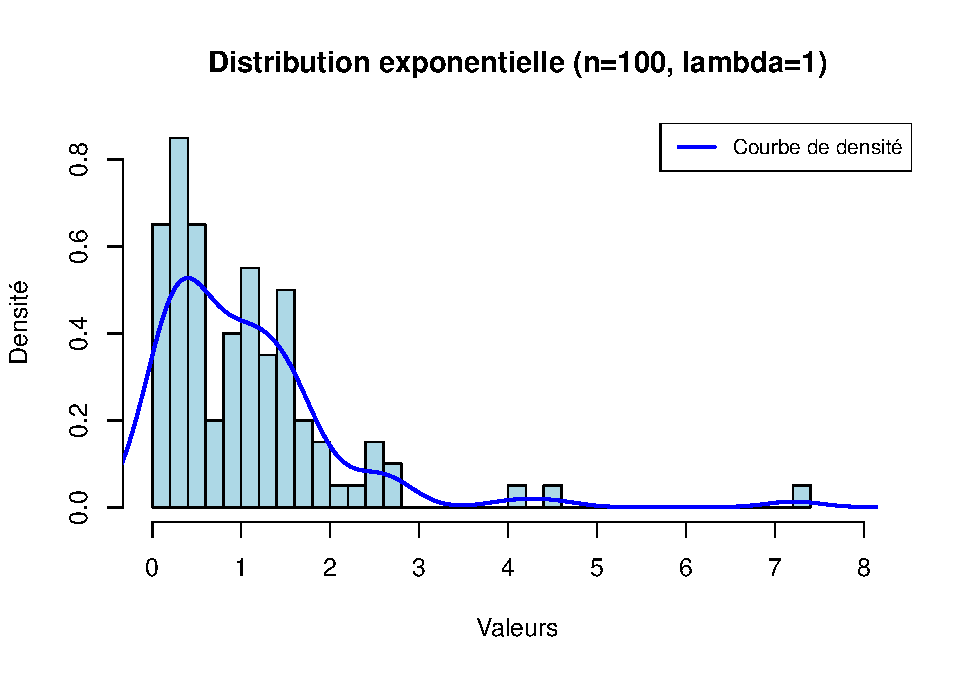
\includegraphics{Stat_non_para_files/figure-latex/unnamed-chunk-4-1.pdf}

\begin{itemize}
\tightlist
\item
  \textbf{Loi de Poisson}
\end{itemize}

\begin{Shaded}
\begin{Highlighting}[]
\CommentTok{\# Histogramme et courbe de densité}

\FunctionTok{hist}\NormalTok{(Echant\_pois, }\AttributeTok{probability =} \ConstantTok{TRUE}\NormalTok{, }\AttributeTok{col =} \StringTok{"lightblue"}\NormalTok{, }
     \AttributeTok{main =} \StringTok{"Distribution de Poisson (n=100, lambda=5)"}\NormalTok{,}
     \AttributeTok{xlab =} \StringTok{"Valeurs"}\NormalTok{, }\AttributeTok{ylab =} \StringTok{"Densité"}\NormalTok{, }\AttributeTok{border =} \StringTok{"black"}\NormalTok{,}
     \AttributeTok{xlim =} \FunctionTok{c}\NormalTok{(}\DecValTok{0}\NormalTok{, }\FunctionTok{max}\NormalTok{(Echant\_pois) }\SpecialCharTok{+} \DecValTok{2}\NormalTok{), }\AttributeTok{breaks =} \FunctionTok{max}\NormalTok{(Echant\_pois) }\SpecialCharTok{+} \DecValTok{1}\NormalTok{)  }

\FunctionTok{lines}\NormalTok{(}\FunctionTok{density}\NormalTok{(Echant\_pois), }\AttributeTok{col =} \StringTok{"blue"}\NormalTok{, }\AttributeTok{lwd =} \DecValTok{2}\NormalTok{) }\CommentTok{\# Courbe de densité  }

\CommentTok{\# Personnalisation de l\textquotesingle{}axe des x}
\FunctionTok{axis}\NormalTok{(}\DecValTok{1}\NormalTok{, }\AttributeTok{at =} \FunctionTok{seq}\NormalTok{(}\DecValTok{0}\NormalTok{, }\FunctionTok{max}\NormalTok{(Echant\_pois) }\SpecialCharTok{+} \DecValTok{2}\NormalTok{, }\AttributeTok{by =} \DecValTok{1}\NormalTok{))  }\CommentTok{\# Graduation tous les 1}

\CommentTok{\# Légende}
\FunctionTok{legend}\NormalTok{(}\StringTok{"topright"}\NormalTok{, }\AttributeTok{legend =} \FunctionTok{c}\NormalTok{(}\StringTok{"Courbe de densité"}\NormalTok{), }
       \AttributeTok{col =} \FunctionTok{c}\NormalTok{(}\StringTok{"blue"}\NormalTok{), }\AttributeTok{lwd =} \DecValTok{2}\NormalTok{, }\AttributeTok{lty =} \FunctionTok{c}\NormalTok{(}\DecValTok{1}\NormalTok{), }\AttributeTok{cex =} \FloatTok{0.8}\NormalTok{)}
\end{Highlighting}
\end{Shaded}

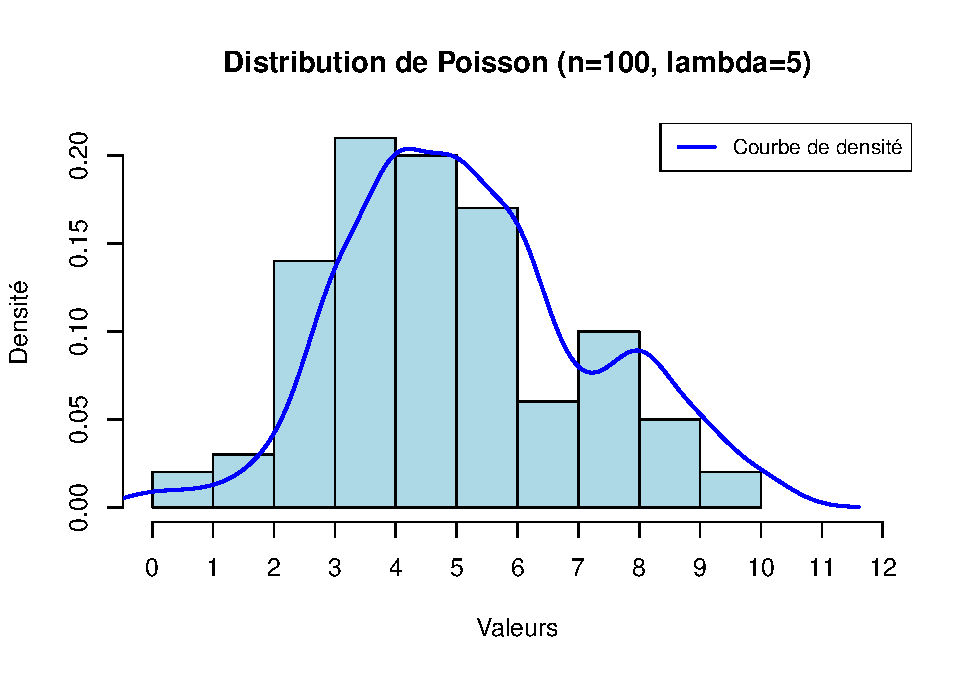
\includegraphics{Stat_non_para_files/figure-latex/unnamed-chunk-5-1.pdf}

\begin{itemize}
\tightlist
\item
  \textbf{Loi de Student}
\end{itemize}

\begin{Shaded}
\begin{Highlighting}[]
\CommentTok{\# Histogramme et courbe de densité}

\FunctionTok{hist}\NormalTok{(Echant\_stud, }\AttributeTok{probability =} \ConstantTok{TRUE}\NormalTok{, }\AttributeTok{col =} \StringTok{"lightblue"}\NormalTok{, }
     \AttributeTok{main =} \StringTok{"Distribution de Student (n=100, ddl=5)"}\NormalTok{,}
     \AttributeTok{xlab =} \StringTok{"Valeurs"}\NormalTok{, }\AttributeTok{ylab =} \StringTok{"Densité"}\NormalTok{, }\AttributeTok{border =} \StringTok{"black"}\NormalTok{,}
     \AttributeTok{xlim =} \FunctionTok{c}\NormalTok{(}\SpecialCharTok{{-}}\DecValTok{6}\NormalTok{, }\DecValTok{5}\NormalTok{), }\AttributeTok{breaks =} \DecValTok{20}\NormalTok{) }

\FunctionTok{lines}\NormalTok{(}\FunctionTok{density}\NormalTok{(Echant\_stud), }\AttributeTok{col =} \StringTok{"blue"}\NormalTok{, }\AttributeTok{lwd =} \DecValTok{2}\NormalTok{) }\CommentTok{\# Courbe de densité empirique}
\FunctionTok{curve}\NormalTok{(}\FunctionTok{dt}\NormalTok{(x, }\AttributeTok{df =} \DecValTok{5}\NormalTok{), }\AttributeTok{col =} \StringTok{"red"}\NormalTok{, }\AttributeTok{lwd =} \DecValTok{2}\NormalTok{, }\AttributeTok{add =} \ConstantTok{TRUE}\NormalTok{, }\AttributeTok{lty =} \DecValTok{2}\NormalTok{) }\CommentTok{\# Densité théorique}

\CommentTok{\# Personnalisation de l\textquotesingle{}axe des x}
\FunctionTok{axis}\NormalTok{(}\DecValTok{1}\NormalTok{, }\AttributeTok{at =} \FunctionTok{seq}\NormalTok{(}\SpecialCharTok{{-}}\DecValTok{6}\NormalTok{, }\DecValTok{5}\NormalTok{, }\AttributeTok{by =} \DecValTok{1}\NormalTok{))  }\CommentTok{\# Ajoute des graduations tous les 1}

\CommentTok{\# Légende}
\FunctionTok{legend}\NormalTok{(}\StringTok{"topright"}\NormalTok{, }\AttributeTok{legend =} \FunctionTok{c}\NormalTok{(}\StringTok{"Densité empirique"}\NormalTok{, }\StringTok{"Densité théorique"}\NormalTok{), }
       \AttributeTok{col =} \FunctionTok{c}\NormalTok{(}\StringTok{"blue"}\NormalTok{, }\StringTok{"red"}\NormalTok{), }\AttributeTok{lwd =} \DecValTok{2}\NormalTok{, }\AttributeTok{lty =} \FunctionTok{c}\NormalTok{(}\DecValTok{1}\NormalTok{,}\DecValTok{2}\NormalTok{), }\AttributeTok{cex =} \FloatTok{0.8}\NormalTok{)}
\end{Highlighting}
\end{Shaded}

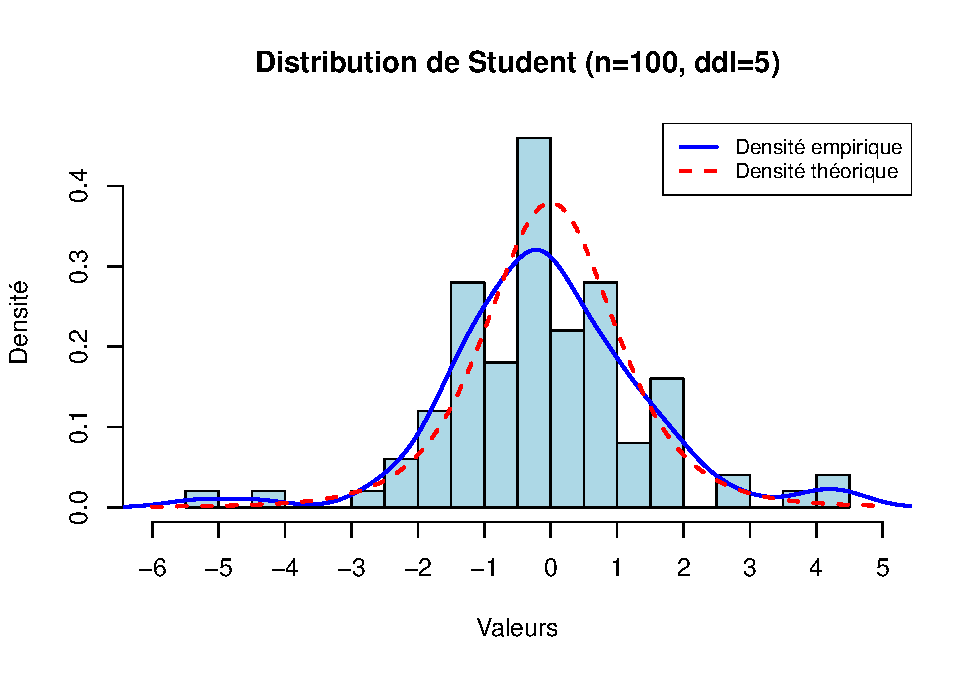
\includegraphics{Stat_non_para_files/figure-latex/unnamed-chunk-6-1.pdf}

\begin{itemize}
\tightlist
\item
  \textbf{Loi géométrique}
\end{itemize}

\begin{Shaded}
\begin{Highlighting}[]
\CommentTok{\#histogramme et courbe de densité}

\FunctionTok{hist}\NormalTok{(Echant\_geo, }\AttributeTok{probability =} \ConstantTok{TRUE}\NormalTok{, }\AttributeTok{col =} \StringTok{"lightblue"}\NormalTok{, }
     \AttributeTok{main =} \StringTok{"Distribution géométrique (n=100, p=0.3)"}\NormalTok{,}
     \AttributeTok{xlab =} \StringTok{"Valeurs"}\NormalTok{, }\AttributeTok{ylab =} \StringTok{"Densité"}\NormalTok{, }\AttributeTok{border =} \StringTok{"black"}\NormalTok{)}

\FunctionTok{lines}\NormalTok{(}\FunctionTok{density}\NormalTok{(Echant\_geo), }\AttributeTok{col =} \StringTok{"blue"}\NormalTok{, }\AttributeTok{lwd =} \DecValTok{2}\NormalTok{) }\CommentTok{\# Courbe de densité}


\FunctionTok{legend}\NormalTok{(}\StringTok{"topright"}\NormalTok{, }\AttributeTok{legend =} \FunctionTok{c}\NormalTok{(}\StringTok{"Courbe de densité"}\NormalTok{), }
       \AttributeTok{col =} \FunctionTok{c}\NormalTok{(}\StringTok{"blue"}\NormalTok{, }\StringTok{"red"}\NormalTok{), }\AttributeTok{lwd =} \DecValTok{2}\NormalTok{, }\AttributeTok{lty =} \FunctionTok{c}\NormalTok{(}\DecValTok{1}\NormalTok{,}\DecValTok{2}\NormalTok{), }\AttributeTok{cex =} \FloatTok{0.4}\NormalTok{)}
\end{Highlighting}
\end{Shaded}

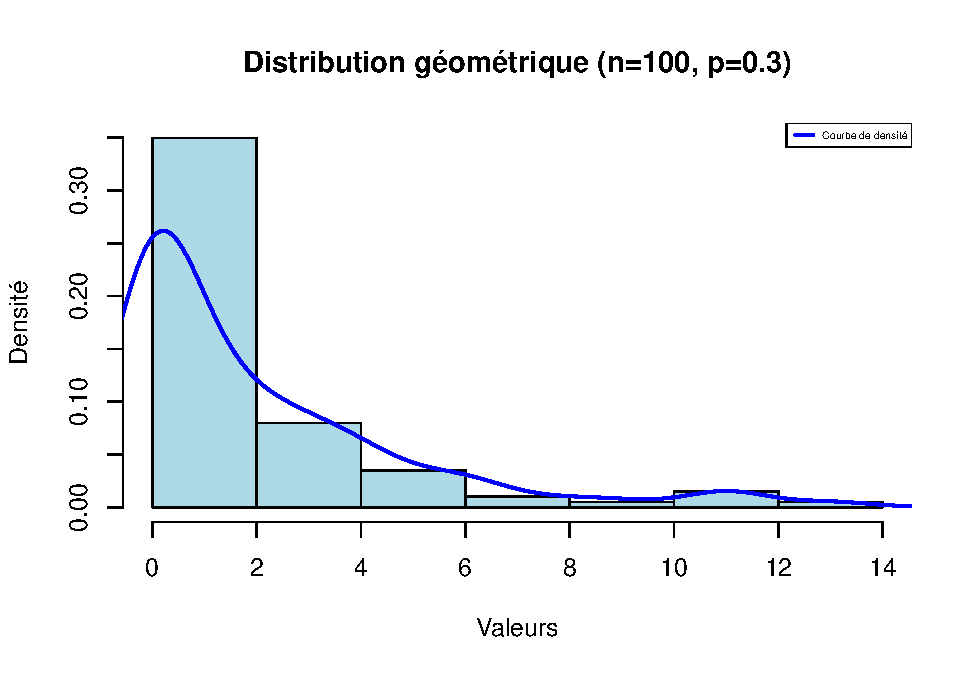
\includegraphics{Stat_non_para_files/figure-latex/unnamed-chunk-7-1.pdf}

\begin{itemize}
\tightlist
\item
  \textbf{Loi normale}
\end{itemize}

\begin{Shaded}
\begin{Highlighting}[]
\CommentTok{\# Histogramme et courbe de densité}

\FunctionTok{hist}\NormalTok{(Echant\_normal, }\AttributeTok{probability =} \ConstantTok{TRUE}\NormalTok{, }\AttributeTok{col =} \StringTok{"lightblue"}\NormalTok{, }
     \AttributeTok{main =} \StringTok{"Distribution d\textquotesingle{}un échantillon normal (n=100)"}\NormalTok{,}
     \AttributeTok{xlab =} \StringTok{"Valeurs"}\NormalTok{, }\AttributeTok{ylab =} \StringTok{"Densité"}\NormalTok{, }\AttributeTok{border =} \StringTok{"black"}\NormalTok{,}
     \AttributeTok{xlim =} \FunctionTok{c}\NormalTok{(}\SpecialCharTok{{-}}\DecValTok{4}\NormalTok{, }\DecValTok{4}\NormalTok{), }\AttributeTok{breaks =} \DecValTok{20}\NormalTok{)  }
\FunctionTok{lines}\NormalTok{(}\FunctionTok{density}\NormalTok{(Echant\_normal), }\AttributeTok{col =} \StringTok{"blue"}\NormalTok{, }\AttributeTok{lwd =} \DecValTok{2}\NormalTok{) }\CommentTok{\# Courbe de densité empirique}

\CommentTok{\# Courbe théorique de la loi normale}
\FunctionTok{curve}\NormalTok{(}\FunctionTok{dnorm}\NormalTok{(x, }\AttributeTok{mean =}\NormalTok{ mu, }\AttributeTok{sd =}\NormalTok{ sigma), }\AttributeTok{col =} \StringTok{"red"}\NormalTok{, }\AttributeTok{lwd =} \DecValTok{2}\NormalTok{, }\AttributeTok{add =} \ConstantTok{TRUE}\NormalTok{, }\AttributeTok{lty =} \DecValTok{2}\NormalTok{)}

\CommentTok{\# Personnalisation de l\textquotesingle{}axe des x}
\FunctionTok{axis}\NormalTok{(}\DecValTok{1}\NormalTok{, }\AttributeTok{at =} \FunctionTok{seq}\NormalTok{(}\SpecialCharTok{{-}}\DecValTok{4}\NormalTok{, }\DecValTok{4}\NormalTok{, }\AttributeTok{by =} \DecValTok{1}\NormalTok{))  }\CommentTok{\# Ajoute des graduations tous les 1}

\CommentTok{\# Légende}
\FunctionTok{legend}\NormalTok{(}\StringTok{"topright"}\NormalTok{, }\AttributeTok{legend =} \FunctionTok{c}\NormalTok{(}\StringTok{"Densité empirique"}\NormalTok{, }\StringTok{"Densité théorique"}\NormalTok{), }
       \AttributeTok{col =} \FunctionTok{c}\NormalTok{(}\StringTok{"blue"}\NormalTok{, }\StringTok{"red"}\NormalTok{), }\AttributeTok{lwd =} \DecValTok{2}\NormalTok{, }\AttributeTok{lty =} \FunctionTok{c}\NormalTok{(}\DecValTok{1}\NormalTok{,}\DecValTok{2}\NormalTok{), }\AttributeTok{cex =} \FloatTok{0.8}\NormalTok{)}
\end{Highlighting}
\end{Shaded}

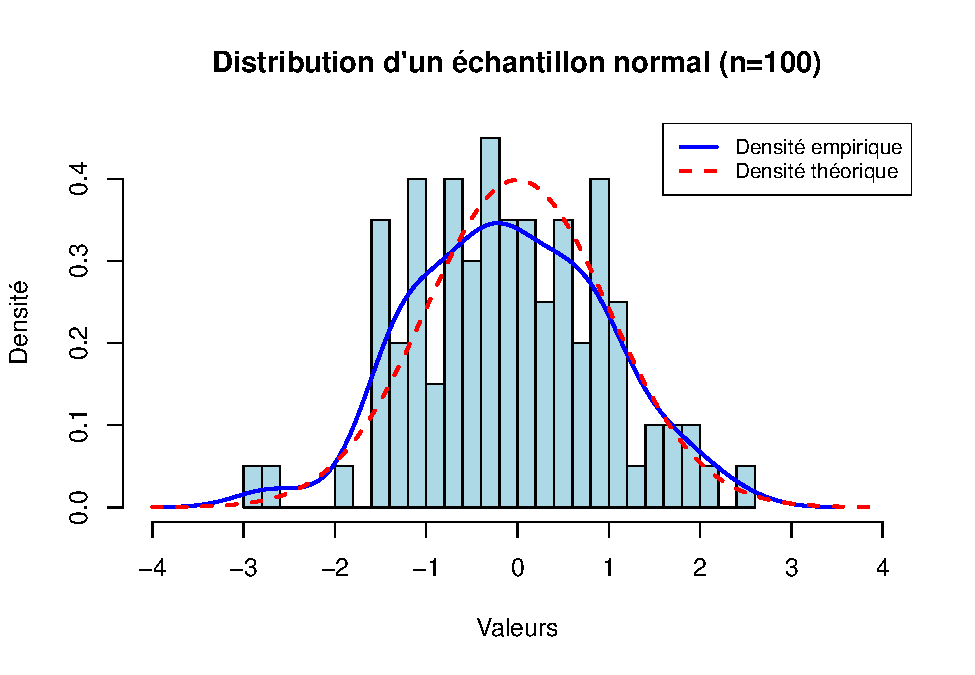
\includegraphics{Stat_non_para_files/figure-latex/unnamed-chunk-8-1.pdf}

\textbf{Conclusion : } La loi de Student a une distribution proche de
celle de loi normale, cela est d'autant plus une realité que les degrés
de liberté sont élevés. La loi de Poisson tend egalement vers la
normalité surtout pour des valeurs de lambda elevés( lambda
\textgreater{} 30). Cependant, les lois exponentielle et géométrique
sont très éloignées d'une distribution normale, elles nécessitent des
transformations pour s'y conformer.

\subsection{Exercice 2 : Statistique
d'ordre}\label{exercice-2-statistique-dordre}

\begin{Shaded}
\begin{Highlighting}[]
\NormalTok{stat\_ordre }\OtherTok{=} \ControlFlowTok{function}\NormalTok{(vector)\{}
              \ControlFlowTok{if}\NormalTok{(}\FunctionTok{is.vector}\NormalTok{(vector)}\SpecialCharTok{==}\ConstantTok{TRUE}\NormalTok{) \{}
\NormalTok{                vect }\OtherTok{=} \FunctionTok{sort}\NormalTok{(vector, }\AttributeTok{decreasing =} \ConstantTok{FALSE}\NormalTok{, }\AttributeTok{na.last =} \ConstantTok{TRUE}\NormalTok{)}
                \FunctionTok{return}\NormalTok{(vect)}
\NormalTok{              \} }\ControlFlowTok{else}\NormalTok{ \{}
                \FunctionTok{print}\NormalTok{(}\StringTok{"Vous devez donner un vecteur"}\NormalTok{)}
\NormalTok{              \}}
\NormalTok{  \}}

\CommentTok{\#Exemple:}
\NormalTok{vec1 }\OtherTok{=} \FunctionTok{c}\NormalTok{(}\DecValTok{5}\NormalTok{,}\DecValTok{2}\NormalTok{,}\SpecialCharTok{{-}}\DecValTok{1}\NormalTok{,}\DecValTok{3}\NormalTok{) }
\NormalTok{a }\OtherTok{=}\FunctionTok{stat\_ordre}\NormalTok{(vec1)}
\FunctionTok{cat}\NormalTok{(}\StringTok{"Vecteur ("}\NormalTok{, vec1, }\StringTok{") "}\NormalTok{, }\StringTok{"ordonné :"}\NormalTok{, a , }\StringTok{"}\SpecialCharTok{\textbackslash{}n}\StringTok{"}\NormalTok{)}
\end{Highlighting}
\end{Shaded}

\begin{verbatim}
## Vecteur ( 5 2 -1 3 )  ordonné : -1 2 3 5
\end{verbatim}

\begin{Shaded}
\begin{Highlighting}[]
\CommentTok{\#Exemple sur un échantillon }
\FunctionTok{set.seed}\NormalTok{(}\DecValTok{123}\NormalTok{) }
\CommentTok{\# échantillon de 50 nombres uniques entre 1 et 100}
\NormalTok{vec2 }\OtherTok{\textless{}{-}} \FunctionTok{sample}\NormalTok{(}\DecValTok{1}\SpecialCharTok{:}\DecValTok{100}\NormalTok{, }\DecValTok{50}\NormalTok{, }\AttributeTok{replace =} \ConstantTok{FALSE}\NormalTok{)  }
\FunctionTok{cat}\NormalTok{(}\StringTok{"Echantillon : "}\NormalTok{, vec2, }\StringTok{"}\SpecialCharTok{\textbackslash{}n}\StringTok{"}\NormalTok{, }\StringTok{"}\SpecialCharTok{\textbackslash{}n}\StringTok{"}\NormalTok{)}
\end{Highlighting}
\end{Shaded}

\begin{verbatim}
## Echantillon :  31 79 51 14 67 42 50 43 97 25 90 69 57 9 72 26 7 95 87 36 78 93 76 15 32 84 82 41 23 27 60 53 75 89 71 38 91 34 29 5 8 12 13 18 33 66 64 65 21 77 
## 
\end{verbatim}

\begin{Shaded}
\begin{Highlighting}[]
\NormalTok{b }\OtherTok{=}\FunctionTok{stat\_ordre}\NormalTok{(vec2)}
\FunctionTok{cat}\NormalTok{( }\StringTok{"Echantillon ordonné : "}\NormalTok{, b )}
\end{Highlighting}
\end{Shaded}

\begin{verbatim}
## Echantillon ordonné :  5 7 8 9 12 13 14 15 18 21 23 25 26 27 29 31 32 33 34 36 38 41 42 43 50 51 53 57 60 64 65 66 67 69 71 72 75 76 77 78 79 82 84 87 89 90 91 93 95 97
\end{verbatim}

\subsection{Exercice 3 : Statistique de
rang}\label{exercice-3-statistique-de-rang}

\begin{Shaded}
\begin{Highlighting}[]
\CommentTok{\#{-}{-}{-}{-}{-}{-}{-}{-}{-}{-}{-}{-}{-}{-}{-}{-}{-}{-}{-}{-}{-}{-}{-}{-}{-}{-}{-}{-}{-}{-}{-}Fonction{-}Rang{-}{-}{-}{-}{-}{-}{-}{-}{-}{-}{-}{-}{-}{-}{-}{-}{-}{-}{-}{-}{-}{-}{-}{-}{-}{-}{-}{-}{-}{-}\#}

\NormalTok{stat\_rang }\OtherTok{\textless{}{-}} \ControlFlowTok{function}\NormalTok{(vector) \{}
  \ControlFlowTok{if}\NormalTok{ (}\SpecialCharTok{!}\FunctionTok{is.vector}\NormalTok{(vector)) \{}
    \FunctionTok{print}\NormalTok{(}\StringTok{"Vous devez donner un vecteur"}\NormalTok{)}
    \FunctionTok{return}\NormalTok{(}\ConstantTok{NULL}\NormalTok{)  }
\NormalTok{  \}}
  
\NormalTok{  vecteur }\OtherTok{\textless{}{-}} \FunctionTok{numeric}\NormalTok{(}\FunctionTok{length}\NormalTok{(vector)) }
  
  \ControlFlowTok{for}\NormalTok{ (i }\ControlFlowTok{in} \DecValTok{1}\SpecialCharTok{:}\FunctionTok{length}\NormalTok{(vector)) \{}
\NormalTok{    compteur }\OtherTok{\textless{}{-}} \DecValTok{0}  
    \ControlFlowTok{for}\NormalTok{ (j }\ControlFlowTok{in} \DecValTok{1}\SpecialCharTok{:}\FunctionTok{length}\NormalTok{(vector)) \{}
      \ControlFlowTok{if}\NormalTok{ (vector[i] }\SpecialCharTok{\textgreater{}=}\NormalTok{ vector[j]) \{}
\NormalTok{        compteur }\OtherTok{\textless{}{-}}\NormalTok{ compteur }\SpecialCharTok{+} \DecValTok{1}
\NormalTok{      \}}
\NormalTok{    \}}
\NormalTok{    vecteur[i] }\OtherTok{\textless{}{-}}\NormalTok{ compteur  }
\NormalTok{  \}}
  \FunctionTok{return}\NormalTok{(vecteur)  }
\NormalTok{\} }
\CommentTok{\#{-}{-}{-}{-}{-}{-}{-}{-}{-}{-}{-}{-}{-}{-}{-}{-}{-}{-}{-}{-}{-}{-}{-}{-}{-}{-}{-}Exemple {-}{-}{-}{-}{-}{-}{-}{-}{-}{-}{-}{-}{-}{-}{-}{-}{-}{-}{-}{-}{-}{-}{-}{-}{-}{-}{-}{-}{-}{-}{-}{-}{-}{-}{-}{-}\#}
\NormalTok{vecteur }\OtherTok{=} \FunctionTok{c}\NormalTok{(}\DecValTok{5}\NormalTok{,}\DecValTok{2}\NormalTok{,}\SpecialCharTok{{-}}\DecValTok{1}\NormalTok{,}\DecValTok{3}\NormalTok{) }
\NormalTok{rang}\OtherTok{=}\FunctionTok{stat\_rang}\NormalTok{(vecteur)}
\NormalTok{rang}
\end{Highlighting}
\end{Shaded}

\begin{verbatim}
## [1] 4 2 1 3
\end{verbatim}

\begin{Shaded}
\begin{Highlighting}[]
\CommentTok{\# Pour un echantillon : }

\FunctionTok{set.seed}\NormalTok{(}\DecValTok{123}\NormalTok{) }
 \CommentTok{\# echantillon de 50 nombres uniques entre 1 et 100}
\NormalTok{echantillon }\OtherTok{\textless{}{-}} \FunctionTok{sample}\NormalTok{(}\DecValTok{1}\SpecialCharTok{:}\DecValTok{100}\NormalTok{, }\DecValTok{50}\NormalTok{, }\AttributeTok{replace =} \ConstantTok{FALSE}\NormalTok{) }
\FunctionTok{print}\NormalTok{(echantillon)}
\end{Highlighting}
\end{Shaded}

\begin{verbatim}
##  [1] 31 79 51 14 67 42 50 43 97 25 90 69 57  9 72 26  7 95 87 36 78 93 76 15 32
## [26] 84 82 41 23 27 60 53 75 89 71 38 91 34 29  5  8 12 13 18 33 66 64 65 21 77
\end{verbatim}

\begin{Shaded}
\begin{Highlighting}[]
\NormalTok{rang\_echantillon }\OtherTok{=}\FunctionTok{stat\_ordre}\NormalTok{(echantillon)}
\NormalTok{rang\_echantillon}
\end{Highlighting}
\end{Shaded}

\begin{verbatim}
##  [1]  5  7  8  9 12 13 14 15 18 21 23 25 26 27 29 31 32 33 34 36 38 41 42 43 50
## [26] 51 53 57 60 64 65 66 67 69 71 72 75 76 77 78 79 82 84 87 89 90 91 93 95 97
\end{verbatim}

\begin{Shaded}
\begin{Highlighting}[]
\CommentTok{\#{-}{-}{-}{-}{-}{-}{-}{-}{-}{-}{-}{-}{-}{-}{-}{-}{-}{-}{-}{-}{-}{-}{-}{-}{-}{-}{-}{-}{-}{-}{-}{-}{-}{-}{-}{-}{-}{-}{-}{-}{-}{-}{-}{-}{-}{-}{-}{-}{-}{-}{-}{-}{-}{-}{-}{-}{-}{-}{-}{-}{-}{-}{-}{-}{-}{-}{-}{-}{-}{-}{-}{-}{-}{-}{-}{-}{-}{-}\#}

\CommentTok{\# Avec la fonction rank  de r}

\NormalTok{vecteur }\OtherTok{=} \FunctionTok{c}\NormalTok{(}\DecValTok{5}\NormalTok{,}\DecValTok{2}\NormalTok{,}\SpecialCharTok{{-}}\DecValTok{1}\NormalTok{,}\DecValTok{3}\NormalTok{)}
\FunctionTok{rank}\NormalTok{(vecteur)}
\end{Highlighting}
\end{Shaded}

\begin{verbatim}
## [1] 4 2 1 3
\end{verbatim}

\begin{Shaded}
\begin{Highlighting}[]
\CommentTok{\# En cas d\textquotesingle{}exoequo}


\NormalTok{vecteur\_2 }\OtherTok{=} \FunctionTok{c}\NormalTok{(}\DecValTok{5}\NormalTok{,}\DecValTok{5}\NormalTok{,}\SpecialCharTok{{-}}\DecValTok{1}\NormalTok{,}\DecValTok{3}\NormalTok{)}
\FunctionTok{rank}\NormalTok{(vecteur\_2,)}
\end{Highlighting}
\end{Shaded}

\begin{verbatim}
## [1] 3.5 3.5 1.0 2.0
\end{verbatim}

\begin{Shaded}
\begin{Highlighting}[]
\DocumentationTok{\#\# Les options : average, first, last, random, max, min}

\NormalTok{x2 }\OtherTok{=} \FunctionTok{c}\NormalTok{(}\DecValTok{5}\NormalTok{,}\DecValTok{5}\NormalTok{,}\SpecialCharTok{{-}}\DecValTok{1}\NormalTok{,}\DecValTok{3}\NormalTok{,}\DecValTok{3}\NormalTok{,}\DecValTok{2}\NormalTok{,}\DecValTok{4}\NormalTok{,}\DecValTok{3}\NormalTok{)}

\DocumentationTok{\#\# ranks without averaging}
\FunctionTok{rank}\NormalTok{(x2, }\AttributeTok{ties.method=} \StringTok{"average"}\NormalTok{) }
\end{Highlighting}
\end{Shaded}

\begin{verbatim}
## [1] 7.5 7.5 1.0 4.0 4.0 2.0 6.0 4.0
\end{verbatim}

\begin{Shaded}
\begin{Highlighting}[]
\FunctionTok{rank}\NormalTok{(x2, }\AttributeTok{ties.method=} \StringTok{"first"}\NormalTok{)  }\CommentTok{\# first occurrence wins}
\end{Highlighting}
\end{Shaded}

\begin{verbatim}
## [1] 7 8 1 3 4 2 6 5
\end{verbatim}

\begin{Shaded}
\begin{Highlighting}[]
\FunctionTok{rank}\NormalTok{(x2, }\AttributeTok{ties.method=} \StringTok{"last"}\NormalTok{)   }\CommentTok{\#  last occurrence wins}
\end{Highlighting}
\end{Shaded}

\begin{verbatim}
## [1] 8 7 1 5 4 2 6 3
\end{verbatim}

\begin{Shaded}
\begin{Highlighting}[]
\FunctionTok{rank}\NormalTok{(x2, }\AttributeTok{ties.method=} \StringTok{"random"}\NormalTok{) }\CommentTok{\# ties broken at random}
\end{Highlighting}
\end{Shaded}

\begin{verbatim}
## [1] 7 8 1 4 5 2 6 3
\end{verbatim}

\begin{Shaded}
\begin{Highlighting}[]
\FunctionTok{rank}\NormalTok{(x2, }\AttributeTok{ties.method=} \StringTok{"random"}\NormalTok{) }\CommentTok{\# and again}
\end{Highlighting}
\end{Shaded}

\begin{verbatim}
## [1] 8 7 1 3 4 2 6 5
\end{verbatim}

NB : Pour avoir le code de la fonction rank par exemple, il faut saisir
la commande \emph{print(rank).}

\subsection{Exercice 4 : Fonction de répartition
empirique}\label{exercice-4-fonction-de-ruxe9partition-empirique}

\begin{Shaded}
\begin{Highlighting}[]
\CommentTok{\# Fonction pour calculer, retourner les valeurs et tracer la fonction de répartition }

\NormalTok{calculer\_et\_tracer\_Fn }\OtherTok{\textless{}{-}} \ControlFlowTok{function}\NormalTok{(vecteur) \{}
  
\NormalTok{  vecteur\_trie }\OtherTok{\textless{}{-}} \FunctionTok{sort}\NormalTok{(vecteur)}
  
\NormalTok{  n }\OtherTok{\textless{}{-}} \FunctionTok{length}\NormalTok{(vecteur)}
  
\NormalTok{  Fn\_values }\OtherTok{\textless{}{-}} \FunctionTok{sapply}\NormalTok{(vecteur\_trie, }\ControlFlowTok{function}\NormalTok{(x) }\FunctionTok{sum}\NormalTok{(vecteur }\SpecialCharTok{\textless{}=}\NormalTok{ x) }\SpecialCharTok{/}\NormalTok{ n)}
  
\NormalTok{  Fn\_data }\OtherTok{\textless{}{-}} \FunctionTok{data.frame}\NormalTok{(}\AttributeTok{x =}\NormalTok{ vecteur\_trie, }\AttributeTok{Fn =}\NormalTok{ Fn\_values)}
  
  \FunctionTok{print}\NormalTok{(}\StringTok{"Valeurs de la fonction de répartition empirique :"}\NormalTok{)}
  \FunctionTok{print}\NormalTok{(Fn\_data)}
  
  \FunctionTok{plot}\NormalTok{(Fn\_data}\SpecialCharTok{$}\NormalTok{x, Fn\_data}\SpecialCharTok{$}\NormalTok{Fn, }\AttributeTok{type =} \StringTok{"s"}\NormalTok{, }\AttributeTok{xlab =} \StringTok{"x"}\NormalTok{, }\AttributeTok{ylab =} \StringTok{"Fn(x)"}\NormalTok{, }
       \AttributeTok{main =} \StringTok{"Fonction de Répartition Empirique"}\NormalTok{)}
  
  \FunctionTok{return}\NormalTok{(Fn\_data)}
\NormalTok{\}}

\CommentTok{\# Exemple d\textquotesingle{}utilisation}

\FunctionTok{set.seed}\NormalTok{(}\DecValTok{123}\NormalTok{)  }
\NormalTok{vecteur }\OtherTok{\textless{}{-}} \FunctionTok{rnorm}\NormalTok{(}\DecValTok{30}\NormalTok{)  }
\NormalTok{resultat }\OtherTok{\textless{}{-}} \FunctionTok{calculer\_et\_tracer\_Fn}\NormalTok{(vecteur)}
\end{Highlighting}
\end{Shaded}

\begin{verbatim}
## [1] "Valeurs de la fonction de répartition empirique :"
##              x         Fn
## 1  -1.96661716 0.03333333
## 2  -1.68669331 0.06666667
## 3  -1.26506123 0.10000000
## 4  -1.13813694 0.13333333
## 5  -1.06782371 0.16666667
## 6  -1.02600445 0.20000000
## 7  -0.72889123 0.23333333
## 8  -0.68685285 0.26666667
## 9  -0.62503927 0.30000000
## 10 -0.56047565 0.33333333
## 11 -0.55584113 0.36666667
## 12 -0.47279141 0.40000000
## 13 -0.44566197 0.43333333
## 14 -0.23017749 0.46666667
## 15 -0.21797491 0.50000000
## 16  0.07050839 0.53333333
## 17  0.11068272 0.56666667
## 18  0.12928774 0.60000000
## 19  0.15337312 0.63333333
## 20  0.35981383 0.66666667
## 21  0.40077145 0.70000000
## 22  0.46091621 0.73333333
## 23  0.49785048 0.76666667
## 24  0.70135590 0.80000000
## 25  0.83778704 0.83333333
## 26  1.22408180 0.86666667
## 27  1.25381492 0.90000000
## 28  1.55870831 0.93333333
## 29  1.71506499 0.96666667
## 30  1.78691314 1.00000000
\end{verbatim}

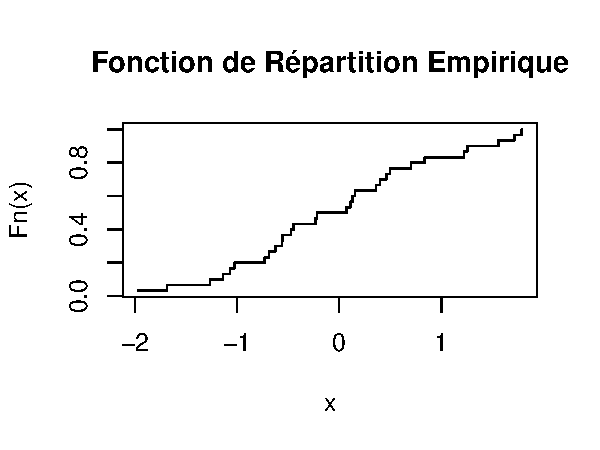
\includegraphics[width=0.8\linewidth]{Stat_non_para_files/figure-latex/unnamed-chunk-13-1}

\begin{Shaded}
\begin{Highlighting}[]
\CommentTok{\# Autre méthode pour tracer la fonction de répartition  et retourner les Fn}

\NormalTok{vecteur }\OtherTok{\textless{}{-}} \FunctionTok{rnorm}\NormalTok{(}\DecValTok{30}\NormalTok{)  }
\FunctionTok{plot}\NormalTok{(}\FunctionTok{ecdf}\NormalTok{(vecteur))}
\end{Highlighting}
\end{Shaded}

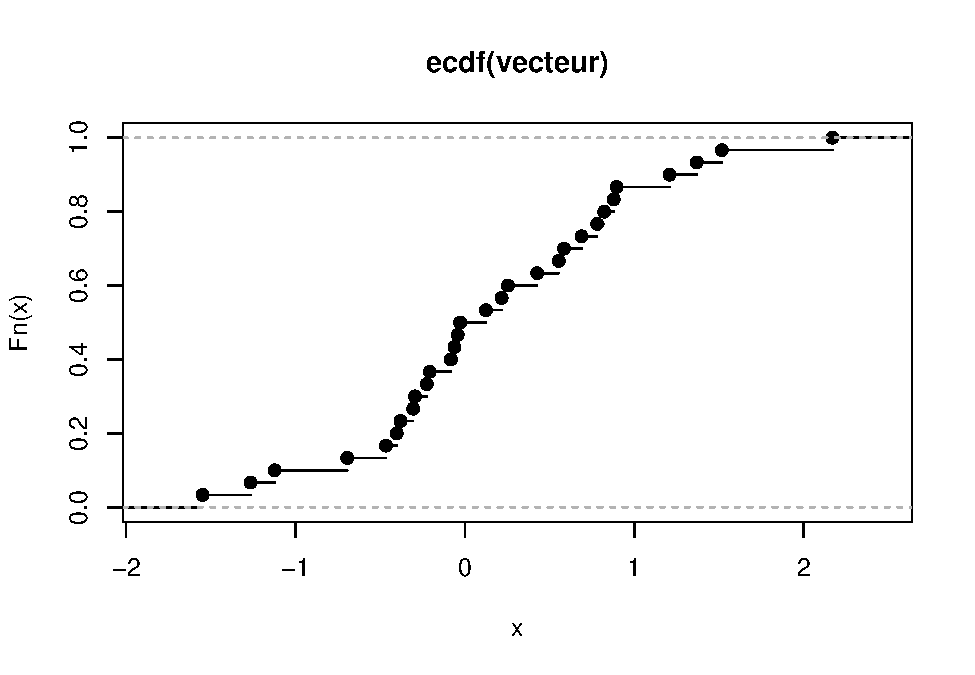
\includegraphics{Stat_non_para_files/figure-latex/unnamed-chunk-14-1.pdf}

\begin{Shaded}
\begin{Highlighting}[]
\FunctionTok{ecdf}\NormalTok{(vecteur)}
\end{Highlighting}
\end{Shaded}

\begin{verbatim}
## Empirical CDF 
## Call: ecdf(vecteur)
##  x[1:30] = -1.5488, -1.2654, -1.1231,  ..., 1.5165,  2.169
\end{verbatim}

\begin{Shaded}
\begin{Highlighting}[]
\NormalTok{fn}\OtherTok{=}\FunctionTok{ecdf}\NormalTok{(vecteur)}
\FunctionTok{fn}\NormalTok{(vecteur)}
\end{Highlighting}
\end{Shaded}

\begin{verbatim}
##  [1] 0.63333333 0.30000000 0.86666667 0.83333333 0.80000000 0.73333333
##  [7] 0.66666667 0.43333333 0.26666667 0.23333333 0.13333333 0.36666667
## [13] 0.06666667 1.00000000 0.90000000 0.10000000 0.20000000 0.16666667
## [19] 0.76666667 0.40000000 0.60000000 0.50000000 0.46666667 0.93333333
## [25] 0.33333333 0.96666667 0.03333333 0.70000000 0.53333333 0.56666667
\end{verbatim}

\begin{Shaded}
\begin{Highlighting}[]
\FunctionTok{fn}\NormalTok{(}\FunctionTok{sort}\NormalTok{(vecteur)) }\CommentTok{\# Pour ordonner les Fn}
\end{Highlighting}
\end{Shaded}

\begin{verbatim}
##  [1] 0.03333333 0.06666667 0.10000000 0.13333333 0.16666667 0.20000000
##  [7] 0.23333333 0.26666667 0.30000000 0.33333333 0.36666667 0.40000000
## [13] 0.43333333 0.46666667 0.50000000 0.53333333 0.56666667 0.60000000
## [19] 0.63333333 0.66666667 0.70000000 0.73333333 0.76666667 0.80000000
## [25] 0.83333333 0.86666667 0.90000000 0.93333333 0.96666667 1.00000000
\end{verbatim}

\newpage

\section{\texorpdfstring{\textcolor{blue}{CHAPITRE 2 : Tests non paramétriques pour 1 échantillon }}{}}\label{section-1}

\subsection{Tests de corrélation de rang de
Spearman}\label{tests-de-corruxe9lation-de-rang-de-spearman}

\subsubsection{On considère les notes de base de données 2 ci-après
:}\label{on-considuxe8re-les-notes-de-base-de-donnuxe9es-2-ci-apruxe8s}

\begin{Shaded}
\begin{Highlighting}[]
\NormalTok{Notes }\OtherTok{\textless{}{-}} \FunctionTok{c}\NormalTok{(}\DecValTok{10}\NormalTok{,}\FloatTok{8.5}\NormalTok{,}\FloatTok{7.5}\NormalTok{,}\FloatTok{8.5}\NormalTok{,}\DecValTok{11}\NormalTok{,}\DecValTok{9}\NormalTok{,}\DecValTok{8}\NormalTok{,}\DecValTok{8}\NormalTok{,}\DecValTok{13}\NormalTok{,}\FloatTok{11.5}\NormalTok{,}\DecValTok{10}\NormalTok{,}\DecValTok{10}\NormalTok{,}\FloatTok{11.5}\NormalTok{,}\FloatTok{11.5}\NormalTok{,}\FloatTok{10.5}\NormalTok{,}\FloatTok{11.5}\NormalTok{,}\DecValTok{14}\NormalTok{,}\DecValTok{6}\NormalTok{,}\DecValTok{6}\NormalTok{,}\FloatTok{9.5}\NormalTok{,}
           \DecValTok{12}\NormalTok{,}\FloatTok{10.5}\NormalTok{,}\DecValTok{9}\NormalTok{,}\FloatTok{11.5}\NormalTok{,}\DecValTok{11}\NormalTok{,}\FloatTok{12.5}\NormalTok{,}\FloatTok{8.5}\NormalTok{,}\DecValTok{11}\NormalTok{,}\DecValTok{13}\NormalTok{,}\DecValTok{6}\NormalTok{,}\FloatTok{9.5}\NormalTok{,}\FloatTok{10.25}\NormalTok{,}\FloatTok{11.5}\NormalTok{,}\DecValTok{10}\NormalTok{,}\FloatTok{11.5}\NormalTok{,}\DecValTok{12}\NormalTok{,}\DecValTok{10}\NormalTok{,}\FloatTok{11.5}\NormalTok{,}
           \DecValTok{12}\NormalTok{,}\FloatTok{9.5}\NormalTok{,}\DecValTok{8}\NormalTok{,}\FloatTok{7.5}\NormalTok{,}\DecValTok{8}\NormalTok{)}
\FunctionTok{plot}\NormalTok{(Notes)}
\end{Highlighting}
\end{Shaded}

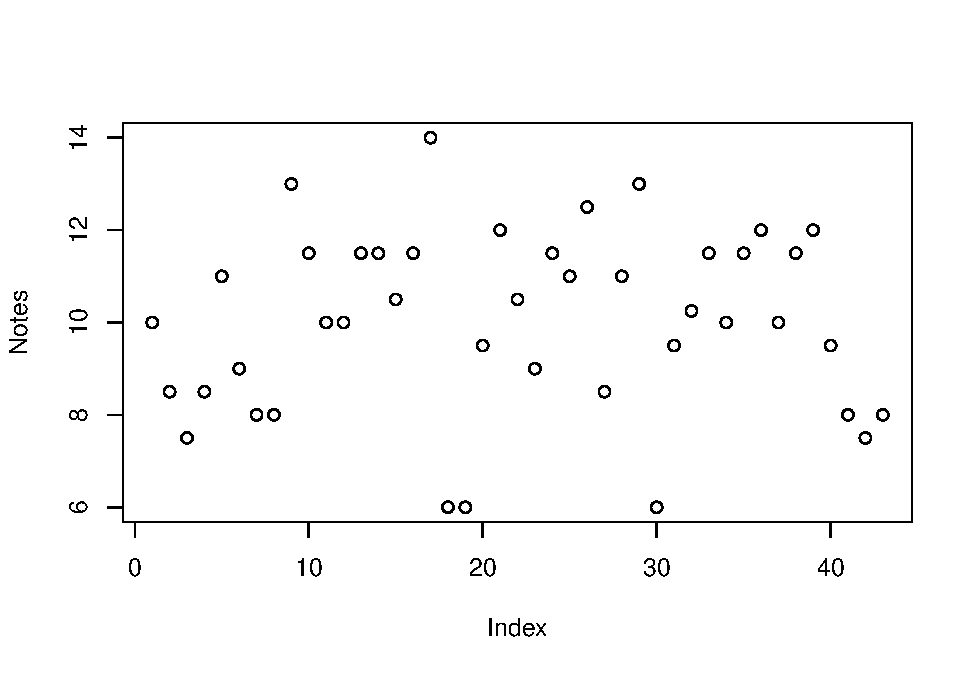
\includegraphics{Stat_non_para_files/figure-latex/unnamed-chunk-15-1.pdf}

\textbf{Commentaires du plot :} Les données semblent homogènes (faible
écart-type et coefficient de variation) et on n'en dégage pas de
tendance a priori. Vérifions cela à l'aide de tests de corrélation de
rangs de Spearman.

\begin{itemize}
\tightlist
\item
  \textbf{Tendance croissante : }
\end{itemize}

On veut tester \(H_0\) : les données sont aléatoires et i.i.d contre
\(H_1\): on a une tendance croissante dans les données.

\begin{Shaded}
\begin{Highlighting}[]
\CommentTok{\# Vecteur rang}
\NormalTok{rang }\OtherTok{\textless{}{-}} \FunctionTok{rank}\NormalTok{(Notes) }
\CommentTok{\# Vecteur d\textquotesingle{}indices}
\NormalTok{i}\OtherTok{=} \DecValTok{1}\SpecialCharTok{:}\FunctionTok{length}\NormalTok{(Notes)}
\CommentTok{\# Dataframe des indices, notes et rangs}
\NormalTok{data }\OtherTok{\textless{}{-}} \FunctionTok{data.frame}\NormalTok{(i, Notes, rang)}
\CommentTok{\#Test de corrélation des rangs de Spearmann}
\FunctionTok{cor.test}\NormalTok{(data}\SpecialCharTok{$}\NormalTok{i, data}\SpecialCharTok{$}\NormalTok{rang, }
         \AttributeTok{alternative=}\StringTok{"g"}\NormalTok{, }\CommentTok{\#tendance croissante}
         \AttributeTok{method=}\StringTok{"spearman"}\NormalTok{ )}
\end{Highlighting}
\end{Shaded}

\begin{verbatim}
## 
##  Spearman's rank correlation rho
## 
## data:  data$i and data$rang
## S = 12179, p-value = 0.3042
## alternative hypothesis: true rho is greater than 0
## sample estimates:
##        rho 
## 0.08038061
\end{verbatim}

\(r_s\) vaut \textbf{0.08} et la p-value est de \textbf{0.3}. On ne peut
rejeter \(H_0\) au seuil de 5\%.

\textbf{NB :} \(S = \sum_{i=1}^{n} \left(R_i - i\right)^2 = 12179\)

\begin{itemize}
\tightlist
\item
  \textbf{Tendance décroissante :}
\end{itemize}

On veut tester \(H_0\) : les données sont aléatoires et i.i.d contre
\(H_1\): on a une tendance décroissante dans les données.

\begin{Shaded}
\begin{Highlighting}[]
\FunctionTok{cor.test}\NormalTok{ (data}\SpecialCharTok{$}\NormalTok{i, data}\SpecialCharTok{$}\NormalTok{Notes, }\AttributeTok{alternative =} \StringTok{"l"}\NormalTok{, }\AttributeTok{method=} \StringTok{"s"}\NormalTok{)}
\end{Highlighting}
\end{Shaded}

\begin{verbatim}
## 
##  Spearman's rank correlation rho
## 
## data:  data$i and data$Notes
## S = 12179, p-value = 0.6958
## alternative hypothesis: true rho is less than 0
## sample estimates:
##        rho 
## 0.08038061
\end{verbatim}

\begin{itemize}
\tightlist
\item
  \textbf{Tendance quelconque :}
\end{itemize}

On veut tester \(H_0\) : les données sont aléatoires et i.i.d contre
\(H_1\): on a une tendance quelconque dans les données.

\begin{Shaded}
\begin{Highlighting}[]
\FunctionTok{cor.test}\NormalTok{ (data}\SpecialCharTok{$}\NormalTok{i, data}\SpecialCharTok{$}\NormalTok{Notes, }\AttributeTok{alternative =} \StringTok{"two.sided"}\NormalTok{, }\AttributeTok{method=} \StringTok{"s"}\NormalTok{)}
\end{Highlighting}
\end{Shaded}

\begin{verbatim}
## Warning in cor.test.default(data$i, data$Notes, alternative = "two.sided", :
## Impossible de calculer la p-value exacte avec des ex-aequos
\end{verbatim}

\begin{verbatim}
## 
##  Spearman's rank correlation rho
## 
## data:  data$i and data$Notes
## S = 12179, p-value = 0.6084
## alternative hypothesis: true rho is not equal to 0
## sample estimates:
##        rho 
## 0.08038061
\end{verbatim}

On a les mêmes conclusions dans les 2 derniers cas. On ne peut rejeter
\(H_o\) au seuil de 5\%.

\subsubsection{On considère les 15 premières
observations.}\label{on-considuxe8re-les-15-premiuxe8res-observations.}

\begin{Shaded}
\begin{Highlighting}[]
\NormalTok{data1}\OtherTok{\textless{}{-}}\NormalTok{ data[}\DecValTok{1}\SpecialCharTok{:}\DecValTok{15}\NormalTok{,}\DecValTok{1}\SpecialCharTok{:}\DecValTok{2}\NormalTok{] }
\FunctionTok{plot}\NormalTok{(data1)}
\end{Highlighting}
\end{Shaded}

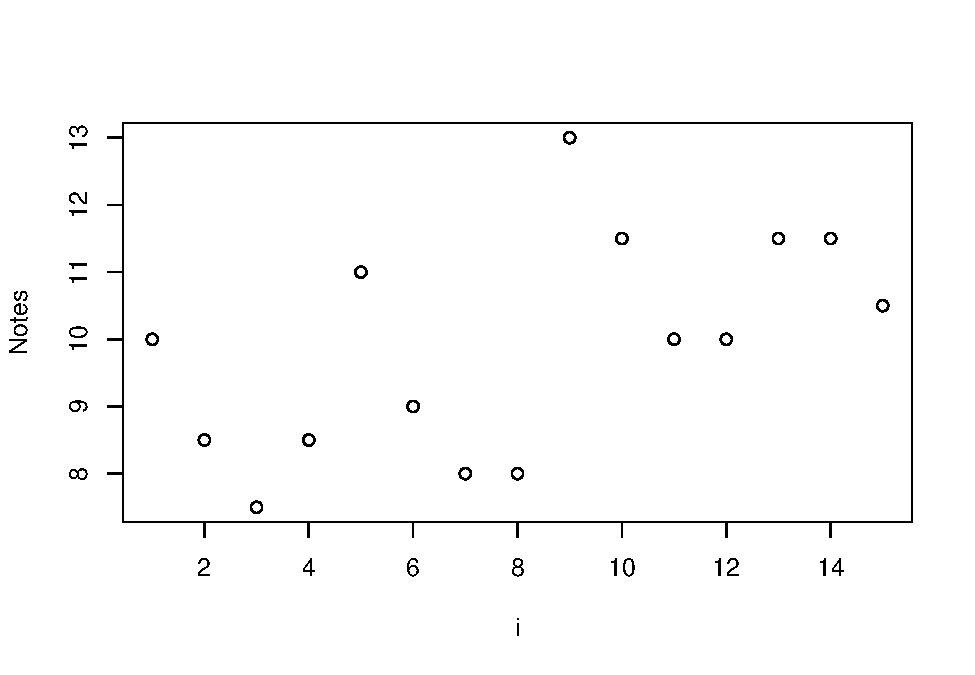
\includegraphics{Stat_non_para_files/figure-latex/unnamed-chunk-19-1.pdf}

Il semblerait y avoir une tendance croissante. Par ailleurs, le nombre
d'observations est inférieur à 30. On ne peut utiliser le cor.test ici.

\begin{Shaded}
\begin{Highlighting}[]
\NormalTok{data1}\SpecialCharTok{$}\NormalTok{rang }\OtherTok{\textless{}{-}} \FunctionTok{rank}\NormalTok{(data1}\SpecialCharTok{$}\NormalTok{Notes)}
\NormalTok{n}\OtherTok{\textless{}{-}} \FunctionTok{length}\NormalTok{(data1}\SpecialCharTok{$}\NormalTok{i)}
\CommentTok{\# calcul de rs}
\NormalTok{somme }\OtherTok{\textless{}{-}}\FunctionTok{sum}\NormalTok{((data1}\SpecialCharTok{$}\NormalTok{rang}\SpecialCharTok{{-}}\NormalTok{data1}\SpecialCharTok{$}\NormalTok{i)}\SpecialCharTok{\^{}}\DecValTok{2}\NormalTok{) }
\NormalTok{rs }\OtherTok{\textless{}{-}} \DecValTok{1}\SpecialCharTok{{-}} \DecValTok{6}\SpecialCharTok{*}\NormalTok{somme}\SpecialCharTok{/}\NormalTok{(n}\SpecialCharTok{*}\NormalTok{(}\SpecialCharTok{{-}}\DecValTok{1} \SpecialCharTok{+}\NormalTok{ n}\SpecialCharTok{\^{}}\DecValTok{2}\NormalTok{ ))}
\CommentTok{\# calcul de rs\textquotesingle{}(que nous notons rs1)}
\NormalTok{rs1 }\OtherTok{\textless{}{-}}\NormalTok{ rs}\SpecialCharTok{*}\FunctionTok{sqrt}\NormalTok{((n}\DecValTok{{-}2}\NormalTok{)}\SpecialCharTok{/}\NormalTok{(}\DecValTok{1}\SpecialCharTok{{-}}\NormalTok{rs}\SpecialCharTok{\^{}}\DecValTok{2}\NormalTok{))}
\CommentTok{\#t de Student pour rs1}
\NormalTok{t}\OtherTok{\textless{}{-}} \FunctionTok{qt}\NormalTok{(}\FloatTok{0.95}\NormalTok{,}\DecValTok{13}\NormalTok{)}
\CommentTok{\#Affichage des résultats}
\FunctionTok{cat}\NormalTok{(}\StringTok{"rs = "}\NormalTok{, rs, }\StringTok{"}\SpecialCharTok{\textbackslash{}n}\StringTok{"}\NormalTok{)}
\end{Highlighting}
\end{Shaded}

\begin{verbatim}
## rs =  0.5678571
\end{verbatim}

\begin{Shaded}
\begin{Highlighting}[]
\FunctionTok{cat}\NormalTok{(}\StringTok{"rs\textquotesingle{} = "}\NormalTok{, rs1, }\StringTok{"}\SpecialCharTok{\textbackslash{}n}\StringTok{"}\NormalTok{)}
\end{Highlighting}
\end{Shaded}

\begin{verbatim}
## rs' =  2.48739
\end{verbatim}

\begin{Shaded}
\begin{Highlighting}[]
\FunctionTok{cat}\NormalTok{(}\StringTok{"t (13, 0.95) = "}\NormalTok{, t, }\StringTok{"}\SpecialCharTok{\textbackslash{}n}\StringTok{"}\NormalTok{)}
\end{Highlighting}
\end{Shaded}

\begin{verbatim}
## t (13, 0.95) =  1.770933
\end{verbatim}

On obtient que \(rs' > t\). Au vu de l'évidence des données, on peut
rejeter \(H_0\) au seuil de 5\%.

\subsection{Test de Kendall}\label{test-de-kendall}

\subsubsection{Données}\label{donnuxe9es}

Le test de Kendall permet de repérer une tendance dans un ensemble de
données, sans supposer que celles-ci suivent une loi normale. Il se base
sur les rangs pour mesurer s'il y a une progression ou une diminution
régulière.

À partir des données fournies dans l'exercice du cours, nous allons
appliquer ce test pour voir s'il existe une tendance significative

\begin{Shaded}
\begin{Highlighting}[]
\NormalTok{vecteur2}\OtherTok{=}\FunctionTok{c}\NormalTok{(}\FloatTok{8.1}\NormalTok{,}\FloatTok{7.3}\NormalTok{,}\FloatTok{6.4}\NormalTok{,}\FloatTok{5.1}\NormalTok{,}\FloatTok{5.4}\NormalTok{,}\FloatTok{4.3}\NormalTok{,}\FloatTok{3.8}\NormalTok{,}\FloatTok{4.9}\NormalTok{,}\FloatTok{5.2}\NormalTok{,}\FloatTok{6.5}\NormalTok{,}\FloatTok{7.8}\NormalTok{,}\FloatTok{7.6}\NormalTok{,}\FloatTok{9.3}\NormalTok{)}

\NormalTok{inversion }\OtherTok{\textless{}{-}} \ControlFlowTok{function}\NormalTok{(vecteur)\{}
\NormalTok{  n}\OtherTok{=}\FunctionTok{length}\NormalTok{(vecteur)}
\NormalTok{  total }\OtherTok{\textless{}{-}}\DecValTok{0}
\NormalTok{  total2 }\OtherTok{\textless{}{-}}\DecValTok{0}
  \ControlFlowTok{for}\NormalTok{ (i }\ControlFlowTok{in} \DecValTok{1}\SpecialCharTok{:}\NormalTok{(n}\DecValTok{{-}1}\NormalTok{)) \{}
\NormalTok{    som1 }\OtherTok{\textless{}{-}} \DecValTok{0}
\NormalTok{    som2 }\OtherTok{\textless{}{-}} \DecValTok{0}
    \ControlFlowTok{for}\NormalTok{ (j }\ControlFlowTok{in}\NormalTok{ (i}\SpecialCharTok{+}\DecValTok{1}\NormalTok{)}\SpecialCharTok{:}\NormalTok{n) \{}
      \ControlFlowTok{if}\NormalTok{ (vecteur[i] }\SpecialCharTok{\textgreater{}}\NormalTok{ vecteur[j]) \{}
\NormalTok{        som1 }\OtherTok{\textless{}{-}}\NormalTok{ som1 }\SpecialCharTok{+} \DecValTok{1} 
\NormalTok{      \}}
      \ControlFlowTok{if}\NormalTok{ (vecteur[i] }\SpecialCharTok{\textless{}}\NormalTok{ vecteur[j])\{ }
\NormalTok{        som2 }\OtherTok{\textless{}{-}}\NormalTok{ som2 }\SpecialCharTok{+} \DecValTok{1} 
\NormalTok{      \}}
\NormalTok{    \}}
\NormalTok{    total }\OtherTok{\textless{}{-}}\NormalTok{ total }\SpecialCharTok{+}\NormalTok{ som1}
\NormalTok{    total2 }\OtherTok{\textless{}{-}}\NormalTok{ total2 }\SpecialCharTok{+}\NormalTok{ som2}
\NormalTok{  \}}
\NormalTok{  S}\OtherTok{=}\NormalTok{ total2 }\SpecialCharTok{{-}}\NormalTok{ total}
  \FunctionTok{return}\NormalTok{(}\FunctionTok{c}\NormalTok{(total, S, n))}
\NormalTok{\}}

\NormalTok{resultat }\OtherTok{=} \FunctionTok{inversion}\NormalTok{(vecteur2)}
\NormalTok{Q }\OtherTok{\textless{}{-}}\NormalTok{ resultat[}\DecValTok{1}\NormalTok{]}
\NormalTok{S }\OtherTok{\textless{}{-}}\NormalTok{ resultat[}\DecValTok{2}\NormalTok{]}
\NormalTok{n }\OtherTok{\textless{}{-}}\NormalTok{ resultat[}\DecValTok{3}\NormalTok{]}
\end{Highlighting}
\end{Shaded}

\begin{itemize}
\tightlist
\item
  Visualisation des données
\end{itemize}

\begin{Shaded}
\begin{Highlighting}[]
\FunctionTok{plot}\NormalTok{ (}\DecValTok{1}\SpecialCharTok{:}\NormalTok{n, vecteur2, }\AttributeTok{type =} \StringTok{"b"}\NormalTok{, }\AttributeTok{col =} \StringTok{"blue"}\NormalTok{, }\AttributeTok{pch =} \DecValTok{19}\NormalTok{,}
     \AttributeTok{xlab =} \StringTok{"Index"}\NormalTok{, }\AttributeTok{ylab =} \StringTok{"Valeur"}\NormalTok{, }\AttributeTok{main =} \StringTok{"Évolution des valeurs de vecteur2"}\NormalTok{)}
\FunctionTok{lines}\NormalTok{(}\FunctionTok{lowess}\NormalTok{(}\DecValTok{1}\SpecialCharTok{:}\NormalTok{n, vecteur2), }\AttributeTok{col =} \StringTok{"red"}\NormalTok{, }\AttributeTok{lwd =} \DecValTok{2}\NormalTok{)  }\CommentTok{\# Tendance lissée}
\FunctionTok{legend}\NormalTok{(}\StringTok{"topleft"}\NormalTok{, }\AttributeTok{legend =} \FunctionTok{c}\NormalTok{(}\StringTok{"Valeurs"}\NormalTok{, }\StringTok{"Tendance (LOWESS)"}\NormalTok{), }
       \AttributeTok{col =} \FunctionTok{c}\NormalTok{(}\StringTok{"blue"}\NormalTok{, }\StringTok{"red"}\NormalTok{), }\AttributeTok{lwd =} \FunctionTok{c}\NormalTok{(}\DecValTok{1}\NormalTok{, }\DecValTok{2}\NormalTok{), }\AttributeTok{pch =} \FunctionTok{c}\NormalTok{(}\DecValTok{19}\NormalTok{, }\ConstantTok{NA}\NormalTok{), }\AttributeTok{lty =} \FunctionTok{c}\NormalTok{(}\DecValTok{1}\NormalTok{, }\DecValTok{1}\NormalTok{))}
\end{Highlighting}
\end{Shaded}

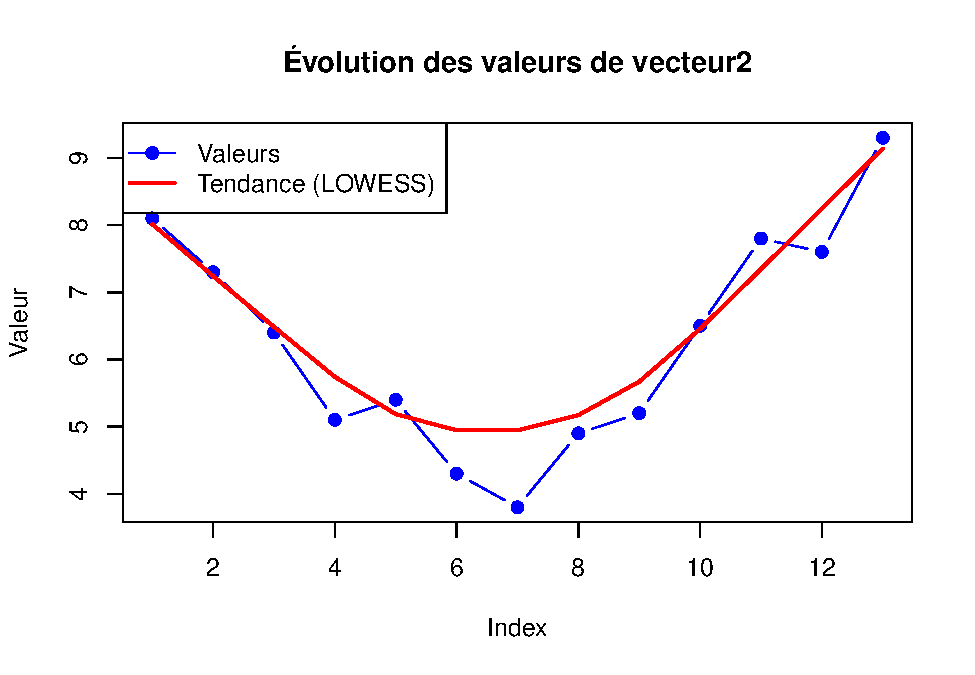
\includegraphics{Stat_non_para_files/figure-latex/unnamed-chunk-22-1.pdf}

\subsubsection{Utilisation de la fonction cor.test avec
Kendall}\label{utilisation-de-la-fonction-cor.test-avec-kendall}

\begin{Shaded}
\begin{Highlighting}[]
\NormalTok{Ri }\OtherTok{=} \FunctionTok{rank}\NormalTok{(vecteur2)}
\NormalTok{i }\OtherTok{=} \DecValTok{1}\SpecialCharTok{:}\NormalTok{n}
\FunctionTok{cor.test}\NormalTok{(Ri, i, }\AttributeTok{alternative =} \StringTok{"greater"}\NormalTok{, }\AttributeTok{method =} \StringTok{"kendall"}\NormalTok{)}
\end{Highlighting}
\end{Shaded}

\begin{verbatim}
## 
##  Kendall's rank correlation tau
## 
## data:  Ri and i
## T = 44, p-value = 0.295
## alternative hypothesis: true tau is greater than 0
## sample estimates:
##       tau 
## 0.1282051
\end{verbatim}

\subsubsection{Espérance et variance de
Q}\label{espuxe9rance-et-variance-de-q}

\begin{itemize}
\item
  \textbf{Formule de calcul de l'espérance :}
  \[ \mathbb{E}[Q]= \dfrac{n(n−1)}{4}\]
\item
  \textbf{Formule de calcul de la variance :}
  \[Var(Q)= \dfrac{n(n−1)(2n+5)}{72}\]
\end{itemize}

\begin{Shaded}
\begin{Highlighting}[]
\NormalTok{E\_Q }\OtherTok{\textless{}{-}}\NormalTok{ n}\SpecialCharTok{*}\NormalTok{(n}\DecValTok{{-}1}\NormalTok{)}\SpecialCharTok{/}\DecValTok{4}
\NormalTok{V\_Q }\OtherTok{\textless{}{-}}\NormalTok{ n}\SpecialCharTok{*}\NormalTok{(n}\DecValTok{{-}1}\NormalTok{)}\SpecialCharTok{*}\NormalTok{(}\DecValTok{2}\SpecialCharTok{*}\NormalTok{n}\SpecialCharTok{+}\DecValTok{5}\NormalTok{)}\SpecialCharTok{/}\DecValTok{72}
\NormalTok{E\_Q; V\_Q}
\end{Highlighting}
\end{Shaded}

\begin{verbatim}
## [1] 39
\end{verbatim}

\begin{verbatim}
## [1] 67.16667
\end{verbatim}

\subsubsection{Tau de Kendall}\label{tau-de-kendall}

\begin{itemize}
\tightlist
\item
  \textbf{Formule de Calcul du tau de Kendall : }
\end{itemize}

\[\tau = \dfrac{1 - 4Q}{n(n - 1)}\]

\begin{itemize}
\item
  \textbf{Espérance du tau de kendall :} \[\mathbb {E} [\tau] = 0\]
\item
  \textbf{Variance du taux :} \[Var(\tau)= \dfrac{2(2n+5)}{9n(n−1)}\]
\end{itemize}

\begin{Shaded}
\begin{Highlighting}[]
\NormalTok{tau }\OtherTok{=} \DecValTok{1} \SpecialCharTok{{-}} \DecValTok{4}\SpecialCharTok{*}\NormalTok{Q }\SpecialCharTok{/}\NormalTok{ (n}\SpecialCharTok{*}\NormalTok{(n}\DecValTok{{-}1}\NormalTok{))}
\NormalTok{E\_tau }\OtherTok{=} \DecValTok{0}
\NormalTok{V\_tau }\OtherTok{=} \DecValTok{2}\SpecialCharTok{*}\NormalTok{(}\DecValTok{2}\SpecialCharTok{*}\NormalTok{n}\SpecialCharTok{+}\DecValTok{5}\NormalTok{) }\SpecialCharTok{/}\NormalTok{ (}\DecValTok{9}\SpecialCharTok{*}\NormalTok{n}\SpecialCharTok{*}\NormalTok{(n}\DecValTok{{-}1}\NormalTok{))}
\NormalTok{tau; V\_tau}
\end{Highlighting}
\end{Shaded}

\begin{verbatim}
## [1] 0.1282051
\end{verbatim}

\begin{verbatim}
## [1] 0.04415954
\end{verbatim}

\subsubsection{Test statistique}\label{test-statistique}

\begin{itemize}
\tightlist
\item
  \textbf{Méthode 1 : test direct manuel}
\end{itemize}

Statistique de test normalisée :

\[ Z = \dfrac{τ−E[τ]}{ \sqrt{Var(\tau)} }\]

Cette statistique sera comparée par la loi normale \(N(0,1)\) pour
déterminer si l'on rejette l'hypothèse nulle.

\begin{Shaded}
\begin{Highlighting}[]
\NormalTok{tau\_centre }\OtherTok{=}\NormalTok{ (tau }\SpecialCharTok{{-}}\NormalTok{ E\_tau) }\SpecialCharTok{/} \FunctionTok{sqrt}\NormalTok{(V\_tau)}
\NormalTok{tau\_centre}
\end{Highlighting}
\end{Shaded}

\begin{verbatim}
## [1] 0.6100889
\end{verbatim}

\begin{Shaded}
\begin{Highlighting}[]
\ControlFlowTok{if}\NormalTok{ (tau\_centre }\SpecialCharTok{\textgreater{}} \FunctionTok{qnorm}\NormalTok{(}\FloatTok{0.975}\NormalTok{) }\SpecialCharTok{|}\NormalTok{ tau\_centre }\SpecialCharTok{\textless{}} \SpecialCharTok{{-}}\FunctionTok{qnorm}\NormalTok{(}\FloatTok{0.975}\NormalTok{)) \{}
  \StringTok{"On rejette H0 (bilatéral) : tendance significative."}
\NormalTok{\} }\ControlFlowTok{else}\NormalTok{ \{}
  \StringTok{"On ne rejette pas H0 (bilatéral)."}
\NormalTok{\}}
\end{Highlighting}
\end{Shaded}

\begin{verbatim}
## [1] "On ne rejette pas H0 (bilatéral)."
\end{verbatim}

\begin{Shaded}
\begin{Highlighting}[]
\ControlFlowTok{if}\NormalTok{ (tau\_centre }\SpecialCharTok{\textgreater{}} \FunctionTok{qnorm}\NormalTok{(}\FloatTok{0.95}\NormalTok{)) \{}
  \StringTok{"On rejette H0 (unilatéral à droite) : ordre positif significatif."}
\NormalTok{\} }\ControlFlowTok{else}\NormalTok{ \{}
  \StringTok{"On ne rejette pas H0 (unilatéral à droite)."}
\NormalTok{\}}
\end{Highlighting}
\end{Shaded}

\begin{verbatim}
## [1] "On ne rejette pas H0 (unilatéral à droite)."
\end{verbatim}

\begin{itemize}
\tightlist
\item
  \textbf{Méthode 2 : test Kendall intégré}
\end{itemize}

La fonction cor.test() a été utilisée pour estimer la corrélation non
paramétrique de Kendall entre les indices (1 à n) et les valeurs de
vecteur2.

Si la statistique tau est positive, cela suggère une tendance croissante
; si elle est négative, cela indiquerait une tendance décroissante.

Cependant, si la p-value est supérieure au seuil de 5 \%, cette tendance
n'est pas statistiquement significative.

Ainsi, si la p-value dépasse ce seuil, on ne rejette pas l'hypothèse
nulle d'absence de tendance monotone entre les valeurs et leur ordre.

\begin{Shaded}
\begin{Highlighting}[]
\FunctionTok{cor.test}\NormalTok{(}\DecValTok{1}\SpecialCharTok{:}\NormalTok{n, vecteur2, }\AttributeTok{method =} \StringTok{"kendall"}\NormalTok{)}
\end{Highlighting}
\end{Shaded}

\begin{verbatim}
## 
##  Kendall's rank correlation tau
## 
## data:  1:n and vecteur2
## T = 44, p-value = 0.59
## alternative hypothesis: true tau is not equal to 0
## sample estimates:
##       tau 
## 0.1282051
\end{verbatim}

\begin{itemize}
\tightlist
\item
  Calcul de la p-value :
\end{itemize}

\[p-value = 2 \times P(Z>|z_{obs}|)=2  \times (1− Φ(∣Z∣)\]

Si p\_value \textless{} 0.05 : on rejette l'hypothèse nulle au seuil de
5 \% . Il y a une tendance significative dans les données.

Si p\_value \textgreater{} 0.05 : on ne rejette pas \(H_0\). Il n'y a
pas de preuve suffisante d'une tendance monotone dans les observations.

\begin{Shaded}
\begin{Highlighting}[]
\NormalTok{p\_value }\OtherTok{=} \DecValTok{2} \SpecialCharTok{*} \FunctionTok{pnorm}\NormalTok{(tau\_centre, }\AttributeTok{lower.tail =} \ConstantTok{FALSE}\NormalTok{)}
\NormalTok{p\_value}
\end{Highlighting}
\end{Shaded}

\begin{verbatim}
## [1] 0.5418029
\end{verbatim}

\subsection{Test de signe}\label{test-de-signe}

\subsubsection{Principe}\label{principe}

Le principe de ce test est similaire au test de Kendall. Sous
l'hypothèse d'indépendance et d'identité de distribution (i.i.d.),
i.e.~sous \(H_0\), chaque observation a une chance sur deux de dépasser
l'observation qui la précède :

\[
\mathbb{P}(X_{i+1} > X_i) = \mathbb{P}(X_{i+1} < X_i) = \frac{1}{2}
\]

La statistique de test est définie par :

\(S = \sum_{i=1}^{n-1} \mathbb{I}(X_i > X_{i+1})\)

où \(\mathbb{I}(\cdot)\) est la fonction indicatrice. La statistique
\(S\) représente donc le \textbf{nombre de différences positives
inversées} dans l'échantillon.

\begin{itemize}
\tightlist
\item
  Si \(X_1 < X_2 < \dots < X_n\) (tendance croissante parfaite), alors
  \(S = 0\)
\item
  Si \(X_1 > X_2 > \dots > X_n\) (tendance décroissante parfaite), alors
  \(S = n - 1\)
\end{itemize}

\subsubsection{\texorpdfstring{Loi de \(S\) sous
\(H_0\)}{Loi de S sous H\_0}}\label{loi-de-s-sous-h_0}

\textbf{Espérance :}

\[
\mathbb{E}(S) = \mathbb{E}\left( \sum_{i=1}^{n-1} \mathbb{I}(X_i > X_{i+1}) \right)
= \sum_{i=1}^{n-1} \mathbb{P}(X_i > X_{i+1}) = \frac{n - 1}{2}
\]

En posant \(Z_i = \mathbb{I}(X_i > X_{i+1})\), on a
\(S = \sum_{i=1}^{n-1} Z_i\).

\textbf{Variance :}

\[
\mathbb{V}(S) = \sum_{i=1}^{n-1} \mathbb{V}(Z_i) + \sum_{i \ne j} \mathrm{Cov}(Z_i, Z_j)
\]

Il a été démontré que : \(\mathbb{V}(S) = \frac{n + 1}{12}\)

\subsubsection{\texorpdfstring{Distribution asymptotique de
\(S\)}{Distribution asymptotique de S}}\label{distribution-asymptotique-de-s}

Pour les petits échantillons (\(n \leq 12\)), on utilise la loi exacte
de \(S - \mathbb{E}(S)\), tabulée par \textbf{Moove et Wallis} (voir
aussi table 16 de \textbf{Phillips-Tessi}).

\begin{itemize}
\tightlist
\item
  Lorsque \(n \to \infty\), on a l'approximation normale suivante :
\end{itemize}

\[
\frac{S - \frac{n - 1}{2}}{\sqrt{ \frac{n + 1}{12} }} \sim \mathcal{N}(0, 1)
\]

Avec \textbf{correction de continuité} :

\[
\left| S - \frac{n - 1}{2} - \frac{1}{2} \right| > z_{1 - \frac{\alpha}{2}} \cdot \sqrt{ \frac{n + 1}{12} }
\]

où \(z_{1 - \alpha/2}\) est le quantile de la loi normale tel que :

\[
\mathbb{P}(|Z| > z_{1 - \alpha/2}) = \alpha \quad \text{avec} \quad Z \sim \mathcal{N}(0, 1)
\]

\textbf{Remarque} : la correction de \(-\frac{1}{2}\) est utilisée pour
approximer une loi discrète (ici celle de \(S\)) par une loi continue
(la loi normale).

\[
\mathbb{P}(X_{i+1} > X_i) = \mathbb{P}(X_{i+1} < X_i) = \frac{1}{2}
\]

La statistique de test est définie par :

\[
S = \sum_{i=1}^{n-1} \mathbb{I}(X_i > X_{i+1})
\]

où \(\mathbb{I}(\cdot)\) est la fonction indicatrice. La statistique
\(S\) représente donc le \textbf{nombre de différences positives
inversées} dans l'échantillon.

Si \(X_1 < X_2 < \dots < X_n\) (tendance croissante parfaite), la
statistique de test compte le nombre de différences positives.

\subsubsection{Données et
visualisation}\label{donnuxe9es-et-visualisation}

\begin{Shaded}
\begin{Highlighting}[]
\NormalTok{data}\OtherTok{=}\FunctionTok{c}\NormalTok{(}\FloatTok{8.1}\NormalTok{,}\FloatTok{7.3}\NormalTok{,}\FloatTok{6.4}\NormalTok{,}\FloatTok{5.1}\NormalTok{,}\FloatTok{5.4}\NormalTok{,}\FloatTok{4.3}\NormalTok{,}\FloatTok{3.8}\NormalTok{,}\FloatTok{4.9}\NormalTok{,}\FloatTok{5.2}\NormalTok{,}\FloatTok{6.5}\NormalTok{,}\FloatTok{7.8}\NormalTok{,}\FloatTok{7.6}\NormalTok{,}\FloatTok{9.3}\NormalTok{)}
\NormalTok{data}
\end{Highlighting}
\end{Shaded}

\begin{verbatim}
##  [1] 8.1 7.3 6.4 5.1 5.4 4.3 3.8 4.9 5.2 6.5 7.8 7.6 9.3
\end{verbatim}

\begin{Shaded}
\begin{Highlighting}[]
\FunctionTok{plot}\NormalTok{(data)}
\end{Highlighting}
\end{Shaded}

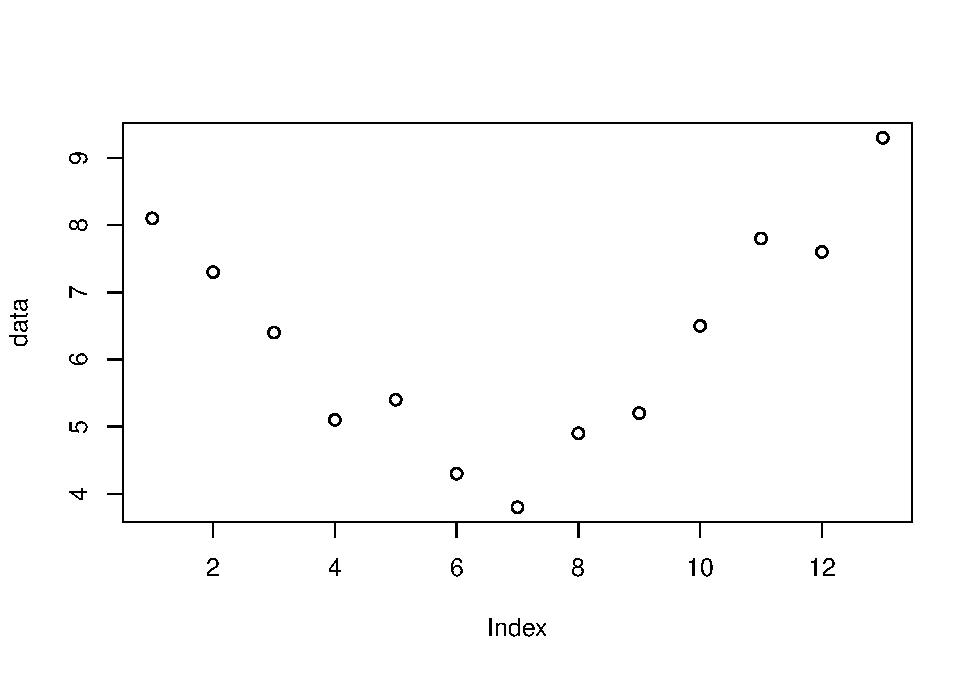
\includegraphics{Stat_non_para_files/figure-latex/unnamed-chunk-30-1.pdf}

\subsubsection{Ecriture de la fonction de statistique de signe
S}\label{ecriture-de-la-fonction-de-statistique-de-signe-s}

\begin{Shaded}
\begin{Highlighting}[]
\NormalTok{Signe }\OtherTok{\textless{}{-}} \ControlFlowTok{function}\NormalTok{(data)\{}
\NormalTok{n}\OtherTok{=}\FunctionTok{length}\NormalTok{(data)}
\NormalTok{total }\OtherTok{\textless{}{-}}\DecValTok{0}
\ControlFlowTok{for}\NormalTok{ (i }\ControlFlowTok{in} \DecValTok{1}\SpecialCharTok{:}\NormalTok{(n}\DecValTok{{-}1}\NormalTok{)) \{}
\ControlFlowTok{if}\NormalTok{ (data[i] }\SpecialCharTok{\textgreater{}}\NormalTok{ data[i}\SpecialCharTok{+}\DecValTok{1}\NormalTok{]) \{}
\NormalTok{total }\OtherTok{\textless{}{-}}\NormalTok{ total }\SpecialCharTok{+} \DecValTok{1}
\NormalTok{\}}
\NormalTok{\}}
\FunctionTok{return}\NormalTok{(total)}
\NormalTok{\}}
\end{Highlighting}
\end{Shaded}

\subsubsection{Application sur les
données}\label{application-sur-les-donnuxe9es}

\begin{Shaded}
\begin{Highlighting}[]
\NormalTok{resultat}\OtherTok{=}\FunctionTok{Signe}\NormalTok{(data)}
\NormalTok{S}\OtherTok{=}\NormalTok{resultat}
\end{Highlighting}
\end{Shaded}

\subsubsection{Calcul de l'Espérance et de la variance de
S}\label{calcul-de-lespuxe9rance-et-de-la-variance-de-s}

\begin{Shaded}
\begin{Highlighting}[]
\NormalTok{n}\OtherTok{=}\FunctionTok{length}\NormalTok{(data)}
\NormalTok{E}\OtherTok{\textless{}{-}}\NormalTok{ (n}\DecValTok{{-}1}\NormalTok{)}\SpecialCharTok{/}\DecValTok{2}
\NormalTok{E}
\end{Highlighting}
\end{Shaded}

\begin{verbatim}
## [1] 6
\end{verbatim}

\begin{Shaded}
\begin{Highlighting}[]
\NormalTok{V }\OtherTok{\textless{}{-}}\NormalTok{ (n}\SpecialCharTok{+}\DecValTok{1}\NormalTok{)}\SpecialCharTok{/}\DecValTok{12}
\NormalTok{V}
\end{Highlighting}
\end{Shaded}

\begin{verbatim}
## [1] 1.166667
\end{verbatim}

On a n =13 \textgreater{} 12 donc on approxime la loi de S par la loi
normale centrée et réduite

\subsubsection{Approximation par la loi
normale}\label{approximation-par-la-loi-normale}

\begin{Shaded}
\begin{Highlighting}[]
\NormalTok{Z }\OtherTok{=}\NormalTok{(S }\SpecialCharTok{{-}}\NormalTok{ E}\SpecialCharTok{{-}}\NormalTok{ (}\DecValTok{1}\SpecialCharTok{/}\DecValTok{2}\NormalTok{))}\SpecialCharTok{/} \FunctionTok{sqrt}\NormalTok{(V)}
\NormalTok{Z}
\end{Highlighting}
\end{Shaded}

\begin{verbatim}
## [1] -0.46291
\end{verbatim}

\begin{itemize}
\tightlist
\item
  \textbf{Pour un test bilateral}
\end{itemize}

\begin{Shaded}
\begin{Highlighting}[]
\ControlFlowTok{if}\NormalTok{ (Z}\SpecialCharTok{\textgreater{}}\FunctionTok{qnorm}\NormalTok{(}\FloatTok{0.975}\NormalTok{, }\DecValTok{0}\NormalTok{,}\DecValTok{1}\NormalTok{) }\SpecialCharTok{|}\NormalTok{ Z }\SpecialCharTok{\textless{}} \SpecialCharTok{{-}}\FunctionTok{qnorm}\NormalTok{(}\FloatTok{0.975}\NormalTok{, }\DecValTok{0}\NormalTok{,}\DecValTok{1}\NormalTok{)) \{}
\StringTok{"On rejette l\textquotesingle{}hypothese nulle : il y a une tendance."}
\NormalTok{\} }\ControlFlowTok{else}\NormalTok{ \{}
\StringTok{"On ne peut pas rejetter l\textquotesingle{}hypothese nulle : pas de tendance ."}
\NormalTok{\}}
\end{Highlighting}
\end{Shaded}

\begin{verbatim}
## [1] "On ne peut pas rejetter l'hypothese nulle : pas de tendance ."
\end{verbatim}

\begin{Shaded}
\begin{Highlighting}[]
\FunctionTok{plot}\NormalTok{(data)}
\end{Highlighting}
\end{Shaded}

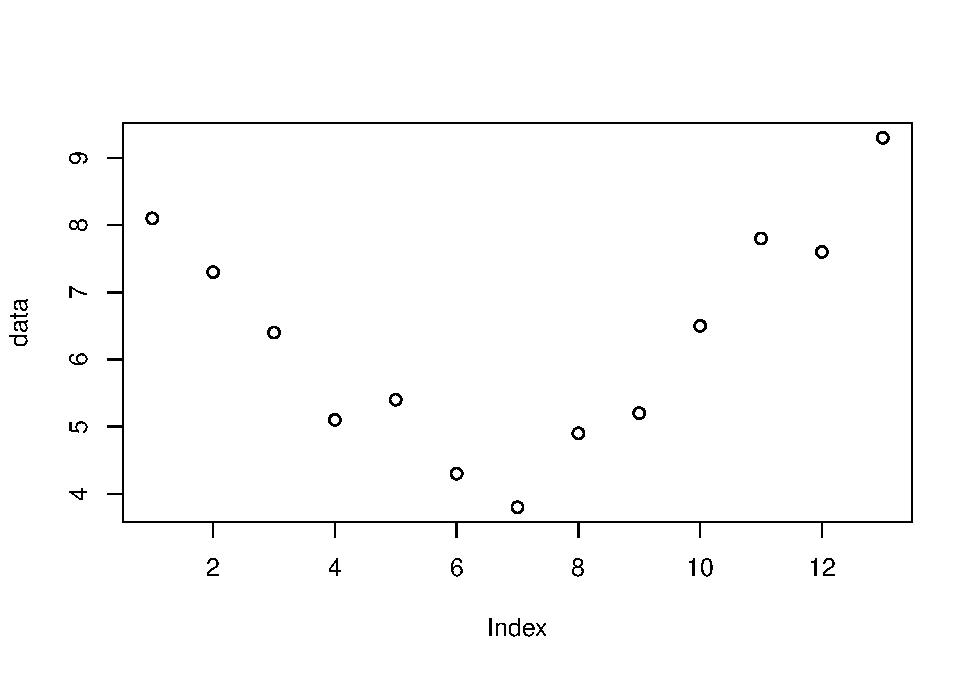
\includegraphics{Stat_non_para_files/figure-latex/unnamed-chunk-37-1.pdf}

\begin{itemize}
\tightlist
\item
  \textbf{Pour un test unilatéral à gauche}
\end{itemize}

\begin{Shaded}
\begin{Highlighting}[]
\ControlFlowTok{if}\NormalTok{ (Z}\SpecialCharTok{\textless{}} \SpecialCharTok{{-}}\FunctionTok{qnorm}\NormalTok{(}\FloatTok{0.95}\NormalTok{, }\DecValTok{0}\NormalTok{,}\DecValTok{1}\NormalTok{) ) \{}
\StringTok{"On rejette l\textquotesingle{}hypothese nulle : dépendance négative."}
\NormalTok{\} }\ControlFlowTok{else}\NormalTok{ \{}
\StringTok{"On ne peut pas rejetter l\textquotesingle{}hypothèse nulle"}
\NormalTok{\}}
\end{Highlighting}
\end{Shaded}

\begin{verbatim}
## [1] "On ne peut pas rejetter l'hypothèse nulle"
\end{verbatim}

\begin{itemize}
\tightlist
\item
  \textbf{Pour un test unilatéral à droite}
\end{itemize}

\begin{Shaded}
\begin{Highlighting}[]
\ControlFlowTok{if}\NormalTok{ (Z}\SpecialCharTok{\textgreater{}}\FunctionTok{qnorm}\NormalTok{(}\FloatTok{0.95}\NormalTok{, }\DecValTok{0}\NormalTok{,}\DecValTok{1}\NormalTok{) ) \{}
\StringTok{"On rejette l\textquotesingle{}hypothese nulle : dépendance positive."}
\NormalTok{\} }\ControlFlowTok{else}\NormalTok{ \{}
\StringTok{"On ne peut pas rejetter l\textquotesingle{}hypothèse nulle"}
\NormalTok{\}}
\end{Highlighting}
\end{Shaded}

\begin{verbatim}
## [1] "On ne peut pas rejetter l'hypothèse nulle"
\end{verbatim}

\textbf{Commentaire :} Dans ces trois cas, Z n'appartient pas à la
région critique Donc on ne peut pas rejetter H0 : iid.

\begin{itemize}
\tightlist
\item
  \textbf{Avec la p-value pour un test bilatéral par exemple}
\end{itemize}

\begin{Shaded}
\begin{Highlighting}[]
\NormalTok{p\_value }\OtherTok{=} \DecValTok{2}\SpecialCharTok{*}\NormalTok{(}\DecValTok{1}\SpecialCharTok{{-}}\FunctionTok{pnorm}\NormalTok{(Z, }\DecValTok{0}\NormalTok{,}\DecValTok{1}\NormalTok{,}\AttributeTok{lower.tail =} \ConstantTok{FALSE}\NormalTok{ ))}
\NormalTok{p\_value}
\end{Highlighting}
\end{Shaded}

\begin{verbatim}
## [1] 0.6434288
\end{verbatim}

\textbf{Conclusion :} Comme la p-value est supérieur à 0.05 , on ne
rejette pas Ho.

\subsection{Test des séquences
homogènes}\label{test-des-suxe9quences-homoguxe8nes}

Une séquence homogène est un groupe consécutif d'éléments identiques
dans une série de données.

Exemple : dans la séquence \texttt{AAABBAAAB}, il y a trois séquences
homogènes : \texttt{AAA}, \texttt{BB}, et \texttt{AAAA}.

Le test des séquences homogènes est utilisé pour déterminer si une série
de données présente une tendance monotone (croissante ou décroissante)
ou si elle est aléatoire.

Les hypothèses du test des séquences homogènes sont les suivantes :

\begin{itemize}
\tightlist
\item
  \(H_0\) : la série de données est aléatoire, sans tendance monotone.
\item
  Alternative unilatérale à droite : \(H_1\) : la série de données est
  croissante.
\item
  Alternative unilatérale à gauche : \(H_1\) : la série de données est
  décroissante.
\item
  Alternative bilatérale : \(H_1\) : la série de données présente une
  tendance monotone quelconque.
\end{itemize}

\subsubsection{Principe du test}\label{principe-du-test}

Si une série de données contient une \textbf{tendance monotone}
(croissante ou décroissante), les valeurs successives auront tendance à
rester \textbf{au-dessus ou en dessous} d'une \textbf{valeur de
référence}. On utilise en général la \textbf{médiane} de la série, notée
\(\lambda\), comme seuil.

On transforme les données selon :

\[
A_i = \begin{cases}
A & \text{si } X_i \geq \lambda \\
B & \text{si } X_i < \lambda
\end{cases}
\]

On dénombre ensuite le \textbf{nombre de séquences homogènes} : ce sont
les blocs consécutifs de A ou de B.

\subsubsection{Données}\label{donnuxe9es-1}

\begin{Shaded}
\begin{Highlighting}[]
\NormalTok{(x }\OtherTok{\textless{}{-}} \FunctionTok{c}\NormalTok{(}\FloatTok{8.1}\NormalTok{, }\FloatTok{7.3}\NormalTok{, }\FloatTok{6.4}\NormalTok{, }\FloatTok{5.1}\NormalTok{, }\FloatTok{5.4}\NormalTok{, }\FloatTok{4.3}\NormalTok{, }\FloatTok{3.8}\NormalTok{, }\FloatTok{4.9}\NormalTok{, }\FloatTok{5.2}\NormalTok{, }\FloatTok{6.5}\NormalTok{, }\FloatTok{7.8}\NormalTok{, }\FloatTok{7.6}\NormalTok{, }\FloatTok{9.3}\NormalTok{))}
\end{Highlighting}
\end{Shaded}

\begin{verbatim}
##  [1] 8.1 7.3 6.4 5.1 5.4 4.3 3.8 4.9 5.2 6.5 7.8 7.6 9.3
\end{verbatim}

\subsubsection{Calcul de la médiane}\label{calcul-de-la-muxe9diane}

\begin{Shaded}
\begin{Highlighting}[]
\NormalTok{(lambda }\OtherTok{\textless{}{-}} \FunctionTok{median}\NormalTok{(x))}
\end{Highlighting}
\end{Shaded}

\begin{verbatim}
## [1] 6.4
\end{verbatim}

\subsubsection{Création de la suite
A/B}\label{cruxe9ation-de-la-suite-ab}

\begin{Shaded}
\begin{Highlighting}[]
\NormalTok{(X\_bin }\OtherTok{\textless{}{-}} \FunctionTok{ifelse}\NormalTok{(x }\SpecialCharTok{\textgreater{}=}\NormalTok{ lambda, }\StringTok{\textquotesingle{}A\textquotesingle{}}\NormalTok{, }\StringTok{\textquotesingle{}B\textquotesingle{}}\NormalTok{))}
\end{Highlighting}
\end{Shaded}

\begin{verbatim}
##  [1] "A" "A" "A" "B" "B" "B" "B" "B" "B" "A" "A" "A" "A"
\end{verbatim}

\begin{Shaded}
\begin{Highlighting}[]
\NormalTok{df }\OtherTok{\textless{}{-}} \FunctionTok{data.frame}\NormalTok{(}\AttributeTok{index =} \DecValTok{1}\SpecialCharTok{:}\FunctionTok{length}\NormalTok{(x), }\AttributeTok{valeur =}\NormalTok{ x, catégorie }\OtherTok{=}\NormalTok{ X\_bin)}
\CommentTok{\# Représentation graphique avec ligne reliant les points}
\FunctionTok{ggplot}\NormalTok{(df, }\FunctionTok{aes}\NormalTok{(}\AttributeTok{x =}\NormalTok{ index, }\AttributeTok{y =}\NormalTok{ valeur, }\AttributeTok{color =}\NormalTok{ catégorie, }\AttributeTok{group =} \DecValTok{1}\NormalTok{)) }\SpecialCharTok{+}
  \FunctionTok{geom\_line}\NormalTok{(}\AttributeTok{color =} \StringTok{"gray50"}\NormalTok{, }\AttributeTok{linewidth =} \DecValTok{1}\NormalTok{) }\SpecialCharTok{+}       \CommentTok{\# Ligne reliant les points}
  \FunctionTok{geom\_point}\NormalTok{(}\AttributeTok{size =} \DecValTok{4}\NormalTok{) }\SpecialCharTok{+}                              \CommentTok{\# Points individuels}
  \FunctionTok{geom\_hline}\NormalTok{(}\AttributeTok{yintercept =}\NormalTok{ lambda, }\AttributeTok{linetype =} \StringTok{"dashed"}\NormalTok{, }\AttributeTok{color =} \StringTok{"black"}\NormalTok{) }\SpecialCharTok{+} \CommentTok{\# Ligne seuil}
  \FunctionTok{annotate}\NormalTok{(}\StringTok{"text"}\NormalTok{, }\AttributeTok{x =} \FunctionTok{length}\NormalTok{(x)}\SpecialCharTok{{-}}\DecValTok{1}\NormalTok{, }\AttributeTok{y =}\NormalTok{ lambda }\SpecialCharTok{+} \FloatTok{0.5}\NormalTok{, }
           \AttributeTok{label =} \FunctionTok{paste}\NormalTok{(}\StringTok{"Seuil ="}\NormalTok{, lambda), }\AttributeTok{hjust =} \DecValTok{1}\NormalTok{) }\SpecialCharTok{+}
  \FunctionTok{labs}\NormalTok{(}\AttributeTok{title =} \StringTok{"Visualisation de la séquence avec seuil (médiane)"}\NormalTok{,}
       \AttributeTok{x =} \StringTok{"Position dans la séquence"}\NormalTok{,}
       \AttributeTok{y =} \StringTok{"Valeur"}\NormalTok{) }\SpecialCharTok{+}
  \FunctionTok{scale\_color\_manual}\NormalTok{(}\AttributeTok{values =} \FunctionTok{c}\NormalTok{(}\StringTok{"blue"}\NormalTok{, }\StringTok{"red"}\NormalTok{)) }\SpecialCharTok{+}
  \FunctionTok{theme\_minimal}\NormalTok{()}
\end{Highlighting}
\end{Shaded}

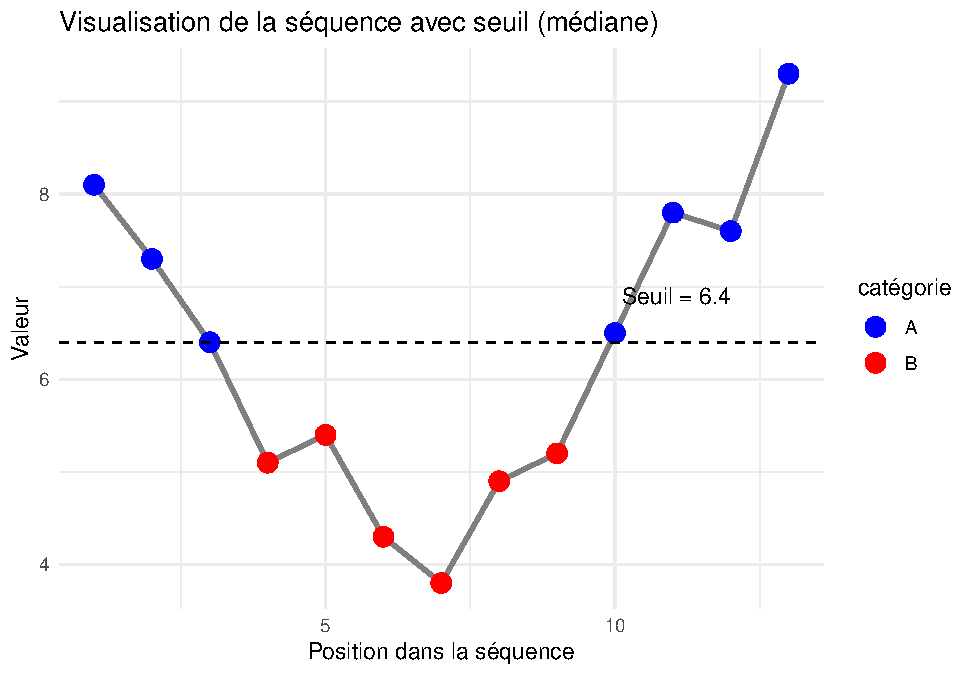
\includegraphics{Stat_non_para_files/figure-latex/unnamed-chunk-44-1.pdf}

D'après la figure on observe de deux séquences homgènes de A et deux
sequences homogènes de B donc notre statistique de test devrait être
égale à 4.

Cependant , formellement , elle est construite de cette manière : On
considère une série \((X_1, X_2, \ldots, X_n)\) et une valeur seuil
\(X_0\).

On définit la variable \(Z_i\) par :

\[
Z_i =
\begin{cases}
1 & \text{si } X_i \text{ et } X_{i+1} \text{ sont différentes (AB ou BA)} \\
0 & \text{sinon (AA ou BB)}
\end{cases}
\]

La statistique de test est donnée par :

\[
S = \sum_{i = 1}^{n - 1} Z_i + 1
\]

avec p le nombre d'éléments de A, m le nombre d'éléments de B et n=m+p .

\subsubsection{Calcul de la Statistique de test : nombre de séquences
homogènes
(S)}\label{calcul-de-la-statistique-de-test-nombre-de-suxe9quences-homoguxe8nes-s}

Ici on compte les changements de groupe (AB ou BA) :

\paragraph{Commençons par calculer p, m, et
n}\label{commenuxe7ons-par-calculer-p-m-et-n}

\begin{Shaded}
\begin{Highlighting}[]
\CommentTok{\# Nombre de séquences homogènes}
\CommentTok{\# p : nombre de A}
\CommentTok{\# m : nombre de B}
\CommentTok{\# n : taille de la séquence}

\NormalTok{p }\OtherTok{\textless{}{-}} \FunctionTok{sum}\NormalTok{(X\_bin }\SpecialCharTok{==} \StringTok{\textquotesingle{}A\textquotesingle{}}\NormalTok{)}
\NormalTok{m }\OtherTok{\textless{}{-}} \FunctionTok{sum}\NormalTok{(X\_bin }\SpecialCharTok{==} \StringTok{\textquotesingle{}B\textquotesingle{}}\NormalTok{)}
\NormalTok{n }\OtherTok{\textless{}{-}} \FunctionTok{length}\NormalTok{(X\_bin)}
\NormalTok{p}
\end{Highlighting}
\end{Shaded}

\begin{verbatim}
## [1] 7
\end{verbatim}

\begin{Shaded}
\begin{Highlighting}[]
\NormalTok{m}
\end{Highlighting}
\end{Shaded}

\begin{verbatim}
## [1] 6
\end{verbatim}

\begin{Shaded}
\begin{Highlighting}[]
\NormalTok{n}
\end{Highlighting}
\end{Shaded}

\begin{verbatim}
## [1] 13
\end{verbatim}

\paragraph{Valeur de la Statistique de
test}\label{valeur-de-la-statistique-de-test}

\begin{Shaded}
\begin{Highlighting}[]
\NormalTok{S }\OtherTok{\textless{}{-}} \DecValTok{1} \SpecialCharTok{+} \FunctionTok{sum}\NormalTok{(}\FunctionTok{as.numeric}\NormalTok{(X\_bin[}\SpecialCharTok{{-}}\DecValTok{1}\NormalTok{] }\SpecialCharTok{!=}\NormalTok{ X\_bin[}\SpecialCharTok{{-}}\NormalTok{n]))}
\NormalTok{S}
\end{Highlighting}
\end{Shaded}

\begin{verbatim}
## [1] 3
\end{verbatim}

Pour de petits échantillons ( p et m inferieur à 20), on utilise la
table de \textbf{Swed et Eisenhart} et pour de grands échantillons, on
utilise l 'approximation avec la loi normale. Cependant même pour de
petits échantillons, on peut faire l'approximation par la loi normale.

Manuellement dans notre cas ou on a m=p=7 et Sur la table de
\textbf{Swed et Eisenhart} on trouve que la region de rejet est
S\textless=4 et S \textgreater=13 donc on rejette l'hypothèse nulle.
Cela signifie que l'échantillon n'est pas iid.

Nous passons ensuite à l'approximation de la loi normale.

\subsubsection{Approximation avec la loi
normale}\label{approximation-avec-la-loi-normale}

\begin{itemize}
\tightlist
\item
  \textbf{Espérance et variance sous Ho}
\end{itemize}

\[
\mathbb{E}(S) = \frac{2pm}{n} + 1
\quad , \quad
\text{Var}(S) = \frac{2pm(2pm - n)}{n^2(n - 1)}
\]

\begin{Shaded}
\begin{Highlighting}[]
\NormalTok{E\_S }\OtherTok{\textless{}{-}} \DecValTok{2} \SpecialCharTok{*}\NormalTok{ p }\SpecialCharTok{*}\NormalTok{ m }\SpecialCharTok{/}\NormalTok{ n }\SpecialCharTok{+} \DecValTok{1}
\NormalTok{Var\_S }\OtherTok{\textless{}{-}}\NormalTok{ (}\DecValTok{2} \SpecialCharTok{*}\NormalTok{ p }\SpecialCharTok{*}\NormalTok{ m }\SpecialCharTok{*}\NormalTok{ (}\DecValTok{2} \SpecialCharTok{*}\NormalTok{ p }\SpecialCharTok{*}\NormalTok{ m }\SpecialCharTok{{-}}\NormalTok{ n)) }\SpecialCharTok{/}\NormalTok{ (n}\SpecialCharTok{\^{}}\DecValTok{2} \SpecialCharTok{*}\NormalTok{ (n }\SpecialCharTok{{-}} \DecValTok{1}\NormalTok{))}
\NormalTok{E\_S}
\end{Highlighting}
\end{Shaded}

\begin{verbatim}
## [1] 7.461538
\end{verbatim}

\begin{Shaded}
\begin{Highlighting}[]
\NormalTok{Var\_S}
\end{Highlighting}
\end{Shaded}

\begin{verbatim}
## [1] 2.940828
\end{verbatim}

\begin{itemize}
\tightlist
\item
  \textbf{Statistique de test (approximation normale)}
\end{itemize}

\[
Z = \frac{S - \mathbb{E}(S)}{\sqrt{\text{Var}(S)}} \sim N(0, 1)
\]

\begin{Shaded}
\begin{Highlighting}[]
\NormalTok{Z }\OtherTok{\textless{}{-}}\NormalTok{ (S }\SpecialCharTok{{-}}\NormalTok{ E\_S) }\SpecialCharTok{/} \FunctionTok{sqrt}\NormalTok{(Var\_S)}
\NormalTok{Z}
\end{Highlighting}
\end{Shaded}

\begin{verbatim}
## [1] -2.601656
\end{verbatim}

\begin{itemize}
\tightlist
\item
  \textbf{p-value bilatérale}
\end{itemize}

\begin{Shaded}
\begin{Highlighting}[]
\DecValTok{2} \SpecialCharTok{*}\NormalTok{ (}\DecValTok{1} \SpecialCharTok{{-}} \FunctionTok{pnorm}\NormalTok{(}\FunctionTok{abs}\NormalTok{(Z)))}
\end{Highlighting}
\end{Shaded}

\begin{verbatim}
## [1] 0.009277498
\end{verbatim}

On rejette \(H_0\) pour alpha= 0.05.

\subsubsection{Test automatisé avec R}\label{test-automatisuxe9-avec-r}

\begin{itemize}
\tightlist
\item
  \textbf{Utilisation du package \texttt{randtests}}
\end{itemize}

\begin{Shaded}
\begin{Highlighting}[]
\FunctionTok{library}\NormalTok{(randtests)}
\end{Highlighting}
\end{Shaded}

\begin{itemize}
\tightlist
\item
  \textbf{Mise en oeuvre du test}
\end{itemize}

Lorsque la moyenne figure parmi les observations, les résultats du test
peuvent différer de ceux de la fonction \texttt{runs.test}, laquelle
scinde les données en comparant strictement chaque valeur à la médiane.

\begin{Shaded}
\begin{Highlighting}[]
\NormalTok{randtests}\SpecialCharTok{::}\FunctionTok{runs.test}\NormalTok{(x, }\AttributeTok{threshold =} \FunctionTok{median}\NormalTok{(x),}
                     \AttributeTok{alternative =} \StringTok{"two.sided"}\NormalTok{, }\AttributeTok{pvalue =} \StringTok{"normal"}\NormalTok{)}
\end{Highlighting}
\end{Shaded}

\begin{verbatim}
## 
##  Runs Test
## 
## data:  x
## statistic = -2.4221, runs = 3, n1 = 6, n2 = 6, n = 12, p-value =
## 0.01543
## alternative hypothesis: nonrandomness
\end{verbatim}

\textbf{Interprétation : } Si la \textbf{p-value est petite}
(\textless{} 0.05), on \textbf{rejette H₀} : présence probable d'une
\textbf{tendance}. Sinon, on \textbf{ne rejette pas H₀} : l'échantillon
est iid.

Comme la p-value est inférieure à 0.05 alors on conclut qu'il y a la
présence d'une tendance monotone.

\textbf{Table de Swed et Eisenhart}

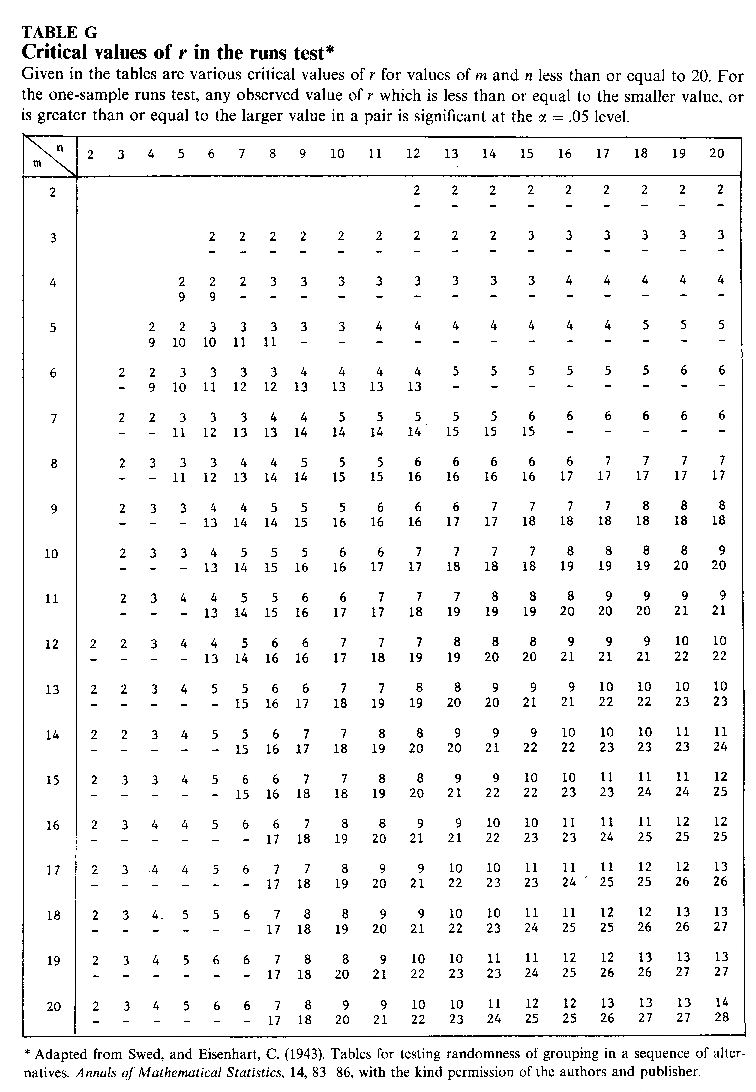
\includepdf[pages=1]{table_sequence_homogene.pdf}

\subsection{Test de localisation : test du
signe}\label{test-de-localisation-test-du-signe}

\begin{Shaded}
\begin{Highlighting}[]
\NormalTok{vecteur }\OtherTok{\textless{}{-}} \FunctionTok{seq}\NormalTok{(}\SpecialCharTok{{-}}\DecValTok{5}\NormalTok{, }\DecValTok{5}\NormalTok{, }\AttributeTok{length.out =} \DecValTok{100}\NormalTok{)}
\end{Highlighting}
\end{Shaded}

\subsubsection{Statistique de test}\label{statistique-de-test}

\begin{Shaded}
\begin{Highlighting}[]
\NormalTok{sta\_test }\OtherTok{\textless{}{-}} \ControlFlowTok{function}\NormalTok{(x) \{}
  \CommentTok{\# Vérifier que c\textquotesingle{}est un vecteur numérique}
  \ControlFlowTok{if}\NormalTok{ (}\SpecialCharTok{!}\FunctionTok{is.numeric}\NormalTok{(x) }\SpecialCharTok{||} \SpecialCharTok{!}\FunctionTok{is.vector}\NormalTok{(x)) \{}
    \FunctionTok{stop}\NormalTok{(}\StringTok{"L\textquotesingle{}entrée doit être un vecteur numérique."}\NormalTok{)}
\NormalTok{  \}}
  
  \CommentTok{\# Calcul des rangs avec moyenne en cas d\textquotesingle{}égalité}
\NormalTok{  rangs }\OtherTok{\textless{}{-}} \FunctionTok{rank}\NormalTok{(x, }\AttributeTok{ties.method =} \StringTok{"average"}\NormalTok{)}
  
  \CommentTok{\# Filtrer les indices des éléments positifs}
\NormalTok{  indices\_positifs }\OtherTok{\textless{}{-}} \FunctionTok{which}\NormalTok{(x }\SpecialCharTok{\textgreater{}} \DecValTok{0}\NormalTok{)}
  
  \CommentTok{\# Extraire les rangs correspondants aux valeurs positives}
\NormalTok{  rangs\_positifs }\OtherTok{\textless{}{-}}\NormalTok{ rangs[indices\_positifs]}
  
  \CommentTok{\# Retourner la somme des valeurs absolues de ces rangs}
  \FunctionTok{return}\NormalTok{(}\FunctionTok{sum}\NormalTok{(}\FunctionTok{abs}\NormalTok{(rangs\_positifs)))}
\NormalTok{\}}
\end{Highlighting}
\end{Shaded}

\subsubsection{Test avec la loi normale}\label{test-avec-la-loi-normale}

\begin{Shaded}
\begin{Highlighting}[]
\CommentTok{\# Fonction principale de test}
\NormalTok{test\_normal }\OtherTok{\textless{}{-}} \ControlFlowTok{function}\NormalTok{(x, }\AttributeTok{alpha =} \FloatTok{0.05}\NormalTok{, }\AttributeTok{type =} \StringTok{"bilateral"}\NormalTok{) \{}
  \ControlFlowTok{if}\NormalTok{ (}\SpecialCharTok{!}\NormalTok{type }\SpecialCharTok{\%in\%} \FunctionTok{c}\NormalTok{(}\StringTok{"bilateral"}\NormalTok{, }\StringTok{"gauche"}\NormalTok{, }\StringTok{"droite"}\NormalTok{)) \{}
    \FunctionTok{stop}\NormalTok{(}\StringTok{"Le type de test doit être \textquotesingle{}bilateral\textquotesingle{}, \textquotesingle{}gauche\textquotesingle{} ou \textquotesingle{}droite\textquotesingle{}."}\NormalTok{)}
\NormalTok{  \}}
  
  \CommentTok{\# Statistique brute}
\NormalTok{  stat }\OtherTok{\textless{}{-}} \FunctionTok{sta\_test}\NormalTok{(x)}
  
  \CommentTok{\# Moyenne et variance de x}
\NormalTok{  moyenne }\OtherTok{\textless{}{-}} \FunctionTok{mean}\NormalTok{(x)}
\NormalTok{  variance }\OtherTok{\textless{}{-}} \FunctionTok{var}\NormalTok{(x)}
  
  \ControlFlowTok{if}\NormalTok{ (variance }\SpecialCharTok{==} \DecValTok{0}\NormalTok{) \{}
    \FunctionTok{stop}\NormalTok{(}\StringTok{"La variance du vecteur est nulle. Le test n\textquotesingle{}est pas applicable."}\NormalTok{)}
\NormalTok{  \}}
  
  \CommentTok{\# Statistique normalisée}
\NormalTok{  T\_stat }\OtherTok{\textless{}{-}}\NormalTok{ (stat }\SpecialCharTok{{-}}\NormalTok{ moyenne) }\SpecialCharTok{/} \FunctionTok{sqrt}\NormalTok{(variance)}
  
  \CommentTok{\# Comparaison selon le type de test}
\NormalTok{  decision }\OtherTok{\textless{}{-}} \StringTok{""}
  \ControlFlowTok{if}\NormalTok{ (type }\SpecialCharTok{==} \StringTok{"bilateral"}\NormalTok{) \{}
\NormalTok{    seuil }\OtherTok{\textless{}{-}} \FunctionTok{qnorm}\NormalTok{(}\DecValTok{1} \SpecialCharTok{{-}}\NormalTok{ alpha }\SpecialCharTok{/} \DecValTok{2}\NormalTok{)}
\NormalTok{    decision }\OtherTok{\textless{}{-}} \FunctionTok{ifelse}\NormalTok{(}\FunctionTok{abs}\NormalTok{(T\_stat) }\SpecialCharTok{\textgreater{}}\NormalTok{ seuil, }\StringTok{"Rejeter H0"}\NormalTok{, }\StringTok{"Ne pas rejeter H0"}\NormalTok{)}
\NormalTok{  \} }\ControlFlowTok{else} \ControlFlowTok{if}\NormalTok{ (type }\SpecialCharTok{==} \StringTok{"droite"}\NormalTok{) \{}
\NormalTok{    seuil }\OtherTok{\textless{}{-}} \FunctionTok{qnorm}\NormalTok{(}\DecValTok{1} \SpecialCharTok{{-}}\NormalTok{ alpha)}
\NormalTok{    decision }\OtherTok{\textless{}{-}} \FunctionTok{ifelse}\NormalTok{(T\_stat }\SpecialCharTok{\textgreater{}}\NormalTok{ seuil, }\StringTok{"Rejeter H0"}\NormalTok{, }\StringTok{"Ne pas rejeter H0"}\NormalTok{)}
\NormalTok{  \} }\ControlFlowTok{else} \ControlFlowTok{if}\NormalTok{ (type }\SpecialCharTok{==} \StringTok{"gauche"}\NormalTok{) \{}
\NormalTok{    seuil }\OtherTok{\textless{}{-}} \FunctionTok{qnorm}\NormalTok{(alpha)}
\NormalTok{    decision }\OtherTok{\textless{}{-}} \FunctionTok{ifelse}\NormalTok{(T\_stat }\SpecialCharTok{\textless{}}\NormalTok{ seuil, }\StringTok{"Rejeter H0"}\NormalTok{, }\StringTok{"Ne pas rejeter H0"}\NormalTok{)}
\NormalTok{  \}}
  
  \CommentTok{\# Résultat}
  \FunctionTok{return}\NormalTok{(}\FunctionTok{list}\NormalTok{(}
    \AttributeTok{statistique =}\NormalTok{ T\_stat,}
    \AttributeTok{seuil =}\NormalTok{ seuil,}
    \AttributeTok{decision =}\NormalTok{ decision}
\NormalTok{  ))}
\NormalTok{\}}
\end{Highlighting}
\end{Shaded}

\begin{Shaded}
\begin{Highlighting}[]
\FunctionTok{test\_normal}\NormalTok{(vecteur)}
\end{Highlighting}
\end{Shaded}

\begin{verbatim}
## $statistique
## [1] 1288.196
## 
## $seuil
## [1] 1.959964
## 
## $decision
## [1] "Rejeter H0"
\end{verbatim}

\subsection{Test de Wilcoxon : avec la fonction de
R}\label{test-de-wilcoxon-avec-la-fonction-de-r}

\begin{Shaded}
\begin{Highlighting}[]
\CommentTok{\# Fonction de test utilisant le test de Wilcoxon}
\NormalTok{test\_wilcoxon }\OtherTok{\textless{}{-}} \ControlFlowTok{function}\NormalTok{(x, }\AttributeTok{alpha =} \FloatTok{0.05}\NormalTok{, }\AttributeTok{type =} \StringTok{"bilateral"}\NormalTok{) \{}
  \ControlFlowTok{if}\NormalTok{ (}\SpecialCharTok{!}\FunctionTok{is.numeric}\NormalTok{(x) }\SpecialCharTok{||} \SpecialCharTok{!}\FunctionTok{is.vector}\NormalTok{(x)) \{}
    \FunctionTok{stop}\NormalTok{(}\StringTok{"L\textquotesingle{}entrée doit être un vecteur numérique."}\NormalTok{)}
\NormalTok{  \}}
  
  \ControlFlowTok{if}\NormalTok{ (}\SpecialCharTok{!}\NormalTok{type }\SpecialCharTok{\%in\%} \FunctionTok{c}\NormalTok{(}\StringTok{"bilateral"}\NormalTok{, }\StringTok{"gauche"}\NormalTok{, }\StringTok{"droite"}\NormalTok{)) \{}
    \FunctionTok{stop}\NormalTok{(}\StringTok{"Le type de test doit être \textquotesingle{}bilateral\textquotesingle{}, \textquotesingle{}gauche\textquotesingle{} ou \textquotesingle{}droite\textquotesingle{}."}\NormalTok{)}
\NormalTok{  \}}
  
  \CommentTok{\# Traduction du type de test pour wilcox.test()}
\NormalTok{  alternative }\OtherTok{\textless{}{-}} \ControlFlowTok{switch}\NormalTok{(type,}
                        \StringTok{"bilateral"} \OtherTok{=} \StringTok{"two.sided"}\NormalTok{,}
                        \StringTok{"gauche"} \OtherTok{=} \StringTok{"less"}\NormalTok{,}
                        \StringTok{"droite"} \OtherTok{=} \StringTok{"greater"}\NormalTok{)}
  
  \CommentTok{\# Test de Wilcoxon signé}
\NormalTok{  test }\OtherTok{\textless{}{-}} \FunctionTok{wilcox.test}\NormalTok{(x, }\AttributeTok{mu =} \DecValTok{0}\NormalTok{, }\AttributeTok{alternative =}\NormalTok{ alternative, }\AttributeTok{exact =} \ConstantTok{FALSE}\NormalTok{, }
                      \AttributeTok{correct =} \ConstantTok{FALSE}\NormalTok{)}
  
  \CommentTok{\# Décision}
\NormalTok{  decision }\OtherTok{\textless{}{-}} \FunctionTok{ifelse}\NormalTok{(test}\SpecialCharTok{$}\NormalTok{p.value }\SpecialCharTok{\textless{}}\NormalTok{ alpha, }\StringTok{"Rejeter H0"}\NormalTok{, }\StringTok{"Ne pas rejeter H0"}\NormalTok{)}
  
  \CommentTok{\# Résultat}
  \FunctionTok{return}\NormalTok{(}\FunctionTok{list}\NormalTok{(}
    \AttributeTok{statistique =}\NormalTok{ test}\SpecialCharTok{$}\NormalTok{statistic,}
    \AttributeTok{p\_value =}\NormalTok{ test}\SpecialCharTok{$}\NormalTok{p.value,}
    \AttributeTok{decision =}\NormalTok{ decision}
\NormalTok{  ))}
\NormalTok{\}}
\end{Highlighting}
\end{Shaded}

\begin{Shaded}
\begin{Highlighting}[]
\FunctionTok{test\_wilcoxon}\NormalTok{(vecteur)}
\end{Highlighting}
\end{Shaded}

\begin{verbatim}
## $statistique
##      V 
## 2519.5 
## 
## $p_value
## [1] 0.984912
## 
## $decision
## [1] "Ne pas rejeter H0"
\end{verbatim}

\newpage

\section{\texorpdfstring{\textcolor{blue}{Chapitre 3 : Tests non paramétriques pour 2 échantillons}}{}}\label{section-2}

\subsection{Tests d'indépendance}\label{tests-dinduxe9pendance}

\subsubsection{Test de Spearman}\label{test-de-spearman}

On dispose de deux échantillons X et Y appariées. On veut tester H0: X
et Y sont indépendants contre H1: X et Y sont dépendants.

La statistique de test considérée est donnée par:

\[ T= \sum_{i=1}^n R_iS_i  \] Avec \(R_i\) et \(S_i\) qui sont les rangs
de l'observation \(i\) dans X et Y.

\begin{itemize}
\tightlist
\item
  \textbf{Fonction manuelle}
\end{itemize}

\begin{Shaded}
\begin{Highlighting}[]
\NormalTok{spearman\_test\_manual }\OtherTok{\textless{}{-}} \ControlFlowTok{function}\NormalTok{(X, Y, }\AttributeTok{alternative =} \StringTok{"two.sided"}\NormalTok{, }\AttributeTok{alpha =} \FloatTok{0.05}\NormalTok{) \{}
\NormalTok{  n }\OtherTok{\textless{}{-}} \FunctionTok{length}\NormalTok{(X)}
  \ControlFlowTok{if}\NormalTok{ (}\FunctionTok{length}\NormalTok{(Y) }\SpecialCharTok{!=}\NormalTok{ n) }\FunctionTok{stop}\NormalTok{(}\StringTok{"Les variables doivent avoir la même longueur"}\NormalTok{)}
  
  \CommentTok{\# 1. Vérification du paramètre alternative}
\NormalTok{  alternative }\OtherTok{\textless{}{-}} \FunctionTok{match.arg}\NormalTok{(alternative, }\FunctionTok{c}\NormalTok{(}\StringTok{"two.sided"}\NormalTok{, }\StringTok{"greater"}\NormalTok{, }\StringTok{"less"}\NormalTok{))}
  
  \CommentTok{\# 2. Calcul des rangs avec gestion des ex{-}aequo}
\NormalTok{  rank\_X }\OtherTok{\textless{}{-}} \FunctionTok{rank}\NormalTok{(X, }\AttributeTok{ties.method =} \StringTok{"average"}\NormalTok{)}
\NormalTok{  rank\_Y }\OtherTok{\textless{}{-}} \FunctionTok{rank}\NormalTok{(Y, }\AttributeTok{ties.method =} \StringTok{"average"}\NormalTok{)}
  
  \CommentTok{\# 3. Calcul de la statistique T = Σ(Ri * Si)}
\NormalTok{  T\_stat }\OtherTok{\textless{}{-}} \FunctionTok{sum}\NormalTok{(rank\_X }\SpecialCharTok{*}\NormalTok{ rank\_Y)}
  
  \CommentTok{\# 4. Correction pour les ex{-}aequo}
\NormalTok{  correct\_ties }\OtherTok{\textless{}{-}} \ControlFlowTok{function}\NormalTok{(ranks) \{}
\NormalTok{    tied\_groups }\OtherTok{\textless{}{-}} \FunctionTok{table}\NormalTok{(ranks)}
    \FunctionTok{sum}\NormalTok{(tied\_groups}\SpecialCharTok{\^{}}\DecValTok{3} \SpecialCharTok{{-}}\NormalTok{ tied\_groups) }\SpecialCharTok{/} \DecValTok{12}
\NormalTok{  \}}
\NormalTok{  TX }\OtherTok{\textless{}{-}} \FunctionTok{correct\_ties}\NormalTok{(rank\_X)}
\NormalTok{  TY }\OtherTok{\textless{}{-}} \FunctionTok{correct\_ties}\NormalTok{(rank\_Y)}
  
  \CommentTok{\# 5. Calcul de la variance}
\NormalTok{  mean\_rank }\OtherTok{\textless{}{-}}\NormalTok{ (n }\SpecialCharTok{+} \DecValTok{1}\NormalTok{)}\SpecialCharTok{/}\DecValTok{2}
\NormalTok{  SS\_R }\OtherTok{\textless{}{-}} \FunctionTok{sum}\NormalTok{(rank\_X}\SpecialCharTok{\^{}}\DecValTok{2}\NormalTok{) }\SpecialCharTok{{-}}\NormalTok{ n }\SpecialCharTok{*}\NormalTok{ mean\_rank}\SpecialCharTok{\^{}}\DecValTok{2}
\NormalTok{  SS\_S }\OtherTok{\textless{}{-}} \FunctionTok{sum}\NormalTok{(rank\_Y}\SpecialCharTok{\^{}}\DecValTok{2}\NormalTok{) }\SpecialCharTok{{-}}\NormalTok{ n }\SpecialCharTok{*}\NormalTok{ mean\_rank}\SpecialCharTok{\^{}}\DecValTok{2}
\NormalTok{  var\_T }\OtherTok{\textless{}{-}}\NormalTok{ (SS\_R}\SpecialCharTok{*}\NormalTok{SS\_S)}\SpecialCharTok{/}\NormalTok{(n}\DecValTok{{-}1}\NormalTok{) }\SpecialCharTok{{-}}\NormalTok{ (TX}\SpecialCharTok{*}\NormalTok{TY)}\SpecialCharTok{/}\NormalTok{(n}\DecValTok{{-}1}\NormalTok{) }\SpecialCharTok{+}\NormalTok{ (TX}\SpecialCharTok{*}\NormalTok{SS\_S }\SpecialCharTok{+}\NormalTok{ TY}\SpecialCharTok{*}\NormalTok{SS\_R)}\SpecialCharTok{/}\NormalTok{(n}\SpecialCharTok{*}\NormalTok{(n}\SpecialCharTok{\^{}}\DecValTok{2} \SpecialCharTok{{-}} \DecValTok{1}\NormalTok{))}
  \CommentTok{\# Note: Sans ex{-}aequo, Var(T) = (SS\_R * SS\_S)/(n{-}1) = n²(n+1)²(n{-}1)/144}
  
  \CommentTok{\# 6. Statistique de test}
\NormalTok{  mu\_T }\OtherTok{\textless{}{-}}\NormalTok{ n }\SpecialCharTok{*}\NormalTok{ mean\_rank}\SpecialCharTok{\^{}}\DecValTok{2}
\NormalTok{  Z }\OtherTok{\textless{}{-}}\NormalTok{ (T\_stat }\SpecialCharTok{{-}}\NormalTok{ mu\_T)}\SpecialCharTok{/}\FunctionTok{sqrt}\NormalTok{(var\_T)}
  
  \CommentTok{\# 7. Calcul du coefficient de Spearman}
\NormalTok{  rho }\OtherTok{\textless{}{-}}\NormalTok{ (}\DecValTok{12} \SpecialCharTok{*}\NormalTok{ (T\_stat }\SpecialCharTok{{-}}\NormalTok{ mu\_T))}\SpecialCharTok{/}\NormalTok{(n}\SpecialCharTok{\^{}}\DecValTok{3} \SpecialCharTok{{-}}\NormalTok{ n }\SpecialCharTok{{-}} \DecValTok{12}\SpecialCharTok{*}\NormalTok{(TX }\SpecialCharTok{+}\NormalTok{ TY) }\SpecialCharTok{+} \DecValTok{12}\SpecialCharTok{*}\NormalTok{(TX}\SpecialCharTok{*}\NormalTok{TY)}\SpecialCharTok{/}\NormalTok{(n}\DecValTok{{-}1}\NormalTok{))}
  
  \CommentTok{\# 8. Valeurs critiques et p{-}value selon l\textquotesingle{}alternative}
  \ControlFlowTok{if}\NormalTok{ (alternative }\SpecialCharTok{==} \StringTok{"two.sided"}\NormalTok{) \{}
\NormalTok{    Z\_critical }\OtherTok{\textless{}{-}} \FunctionTok{qnorm}\NormalTok{(}\DecValTok{1} \SpecialCharTok{{-}}\NormalTok{ alpha}\SpecialCharTok{/}\DecValTok{2}\NormalTok{)}
\NormalTok{    p\_value }\OtherTok{\textless{}{-}} \DecValTok{2} \SpecialCharTok{*} \FunctionTok{pnorm}\NormalTok{(}\SpecialCharTok{{-}}\FunctionTok{abs}\NormalTok{(Z))}
\NormalTok{    decision\_rule }\OtherTok{\textless{}{-}} \FunctionTok{paste}\NormalTok{(}\StringTok{"|Z| \textgreater{}"}\NormalTok{, }\FunctionTok{round}\NormalTok{(Z\_critical, }\DecValTok{4}\NormalTok{))}
\NormalTok{  \} }\ControlFlowTok{else} \ControlFlowTok{if}\NormalTok{ (alternative }\SpecialCharTok{==} \StringTok{"greater"}\NormalTok{) \{}
\NormalTok{    Z\_critical }\OtherTok{\textless{}{-}} \FunctionTok{qnorm}\NormalTok{(}\DecValTok{1} \SpecialCharTok{{-}}\NormalTok{ alpha)}
\NormalTok{    p\_value }\OtherTok{\textless{}{-}} \FunctionTok{pnorm}\NormalTok{(Z, }\AttributeTok{lower.tail =} \ConstantTok{FALSE}\NormalTok{)}
\NormalTok{    decision\_rule }\OtherTok{\textless{}{-}} \FunctionTok{paste}\NormalTok{(}\StringTok{"Z \textgreater{}"}\NormalTok{, }\FunctionTok{round}\NormalTok{(Z\_critical, }\DecValTok{4}\NormalTok{))}
\NormalTok{  \} }\ControlFlowTok{else}\NormalTok{ \{ }\CommentTok{\# "less"}
\NormalTok{    Z\_critical }\OtherTok{\textless{}{-}} \FunctionTok{qnorm}\NormalTok{(alpha)}
\NormalTok{    p\_value }\OtherTok{\textless{}{-}} \FunctionTok{pnorm}\NormalTok{(Z)}
\NormalTok{    decision\_rule }\OtherTok{\textless{}{-}} \FunctionTok{paste}\NormalTok{(}\StringTok{"Z \textless{}"}\NormalTok{, }\FunctionTok{round}\NormalTok{(Z\_critical, }\DecValTok{4}\NormalTok{))}
\NormalTok{  \}}
  
  \CommentTok{\# 9. Décision}
\NormalTok{  decision }\OtherTok{\textless{}{-}} \FunctionTok{ifelse}\NormalTok{(}
\NormalTok{    (alternative }\SpecialCharTok{==} \StringTok{"two.sided"} \SpecialCharTok{\&} \FunctionTok{abs}\NormalTok{(Z) }\SpecialCharTok{\textgreater{}}\NormalTok{ Z\_critical) }\SpecialCharTok{|}
\NormalTok{      (alternative }\SpecialCharTok{==} \StringTok{"greater"} \SpecialCharTok{\&}\NormalTok{ Z }\SpecialCharTok{\textgreater{}}\NormalTok{ Z\_critical) }\SpecialCharTok{|}
\NormalTok{      (alternative }\SpecialCharTok{==} \StringTok{"less"} \SpecialCharTok{\&}\NormalTok{ Z }\SpecialCharTok{\textless{}}\NormalTok{ Z\_critical),}
    \FunctionTok{paste}\NormalTok{(}\StringTok{"Rejeter H0 au seuil"}\NormalTok{, alpha),}
    \FunctionTok{paste}\NormalTok{(}\StringTok{"Ne pas rejeter H0 au seuil"}\NormalTok{, alpha)}
\NormalTok{  )}
  
  \CommentTok{\# Affichage des résultats}
  \FunctionTok{cat}\NormalTok{(}\StringTok{"Test de Spearman Manuel}\SpecialCharTok{\textbackslash{}n}\StringTok{"}\NormalTok{)}
  \FunctionTok{cat}\NormalTok{(}\StringTok{"{-}{-}{-}{-}{-}{-}{-}{-}{-}{-}{-}{-}{-}{-}{-}{-}{-}{-}{-}{-}{-}{-}{-}}\SpecialCharTok{\textbackslash{}n}\StringTok{"}\NormalTok{)}
  \FunctionTok{cat}\NormalTok{(}\StringTok{"Type de test    :"}\NormalTok{, }\ControlFlowTok{switch}\NormalTok{(alternative, }\StringTok{"two.sided"} \OtherTok{=} \StringTok{"Bilatéral (dépendance quelconque)"}\NormalTok{, }\StringTok{"greater"} \OtherTok{=} \StringTok{"Unilatéral droit (dépendance positive)"}\NormalTok{, }\StringTok{"less"} \OtherTok{=} \StringTok{"Unilatéral gauche (dépendance négative)"}\NormalTok{), }\StringTok{"}\SpecialCharTok{\textbackslash{}n}\StringTok{"}\NormalTok{)}
  \FunctionTok{cat}\NormalTok{(}\StringTok{"Statistique T   :"}\NormalTok{, }\FunctionTok{round}\NormalTok{(T\_stat, }\DecValTok{4}\NormalTok{), }\StringTok{"}\SpecialCharTok{\textbackslash{}n}\StringTok{"}\NormalTok{)}
  \FunctionTok{cat}\NormalTok{(}\StringTok{"Statistique Z   :"}\NormalTok{, }\FunctionTok{round}\NormalTok{(Z, }\DecValTok{4}\NormalTok{), }\StringTok{"}\SpecialCharTok{\textbackslash{}n}\StringTok{"}\NormalTok{)}
  \FunctionTok{cat}\NormalTok{(}\StringTok{"Valeur critique :"}\NormalTok{, }\FunctionTok{round}\NormalTok{(Z\_critical, }\DecValTok{4}\NormalTok{), }\StringTok{"}\SpecialCharTok{\textbackslash{}n}\StringTok{"}\NormalTok{)}
  \FunctionTok{cat}\NormalTok{(}\StringTok{"Règle de décision:"}\NormalTok{, decision\_rule, }\StringTok{"}\SpecialCharTok{\textbackslash{}n}\StringTok{"}\NormalTok{)}
  \FunctionTok{cat}\NormalTok{(}\StringTok{"p{-}value         :"}\NormalTok{, }\FunctionTok{sprintf}\NormalTok{(}\StringTok{"\%.6f"}\NormalTok{, p\_value), }\StringTok{"}\SpecialCharTok{\textbackslash{}n}\StringTok{"}\NormalTok{)}
  \FunctionTok{cat}\NormalTok{(}\StringTok{"Coefficient ρ   :"}\NormalTok{, }\FunctionTok{round}\NormalTok{(rho, }\DecValTok{4}\NormalTok{), }\StringTok{"}\SpecialCharTok{\textbackslash{}n}\StringTok{"}\NormalTok{)}
  \FunctionTok{cat}\NormalTok{(}\StringTok{"Décision        :"}\NormalTok{, decision, }\StringTok{"}\SpecialCharTok{\textbackslash{}n}\StringTok{"}\NormalTok{)}
  \FunctionTok{cat}\NormalTok{(}\StringTok{"{-}{-}{-}{-}{-}{-}{-}{-}{-}{-}{-}{-}{-}{-}{-}{-}{-}{-}{-}{-}{-}{-}{-}}\SpecialCharTok{\textbackslash{}n}\StringTok{"}\NormalTok{)}
  
  \FunctionTok{return}\NormalTok{(}\FunctionTok{list}\NormalTok{(}
    \AttributeTok{alternative =}\NormalTok{ alternative,}
    \AttributeTok{T\_stat =}\NormalTok{ T\_stat,}
    \AttributeTok{Z =}\NormalTok{ Z,}
    \AttributeTok{Z\_critical =}\NormalTok{ Z\_critical,}
    \AttributeTok{p\_value =}\NormalTok{ p\_value,}
    \AttributeTok{rho =}\NormalTok{ rho,}
    \AttributeTok{decision =}\NormalTok{ decision}
\NormalTok{  ))}
\NormalTok{\}}
\end{Highlighting}
\end{Shaded}

\begin{itemize}
\tightlist
\item
  \textbf{Exemple d'application et comparaison avec la fonction intégrée
  de R}
\end{itemize}

Ce test doit normalement être effectué avec au moins 30 observations.
mais nous utilisons juste les données de l'exemple d'application du
cours ici.

\begin{itemize}
\tightlist
\item
  \textbf{Données et visualisation}
\end{itemize}

\begin{Shaded}
\begin{Highlighting}[]
\CommentTok{\# {-}{-}{-}{-}{-}{-}{-}{-}{-}{-}{-}{-}{-}{-}{-}{-}{-}{-}{-}{-}{-}{-}{-}{-}{-}{-}{-}{-}}
\CommentTok{\# 1. Données de l\textquotesingle{}application du cours}
\CommentTok{\# {-}{-}{-}{-}{-}{-}{-}{-}{-}{-}{-}{-}{-}{-}{-}{-}{-}{-}{-}{-}{-}{-}{-}{-}{-}{-}{-}{-}}

\NormalTok{data }\OtherTok{\textless{}{-}} \FunctionTok{data.frame}\NormalTok{(}
  \AttributeTok{ID=} \FunctionTok{c}\NormalTok{(}\DecValTok{1}\NormalTok{,}\DecValTok{2}\NormalTok{,}\DecValTok{3}\NormalTok{,}\DecValTok{4}\NormalTok{,}\DecValTok{5}\NormalTok{,}\DecValTok{6}\NormalTok{,}\DecValTok{7}\NormalTok{,}\DecValTok{8}\NormalTok{,}\DecValTok{9}\NormalTok{,}\DecValTok{10}\NormalTok{,}\DecValTok{11}\NormalTok{,}\DecValTok{12}\NormalTok{),}
  \AttributeTok{X=} \FunctionTok{c}\NormalTok{(}\DecValTok{1}\NormalTok{,}\DecValTok{1}\NormalTok{,}\DecValTok{2}\NormalTok{,}\DecValTok{2}\NormalTok{,}\DecValTok{3}\NormalTok{,}\DecValTok{4}\NormalTok{,}\DecValTok{5}\NormalTok{,}\DecValTok{6}\NormalTok{,}\DecValTok{7}\NormalTok{,}\DecValTok{8}\NormalTok{,}\DecValTok{8}\NormalTok{,}\DecValTok{12}\NormalTok{),}
  \AttributeTok{Y=} \FunctionTok{c}\NormalTok{(}\DecValTok{12}\NormalTok{,}\DecValTok{16}\NormalTok{,}\DecValTok{9}\NormalTok{,}\DecValTok{7}\NormalTok{,}\DecValTok{35}\NormalTok{,}\DecValTok{58}\NormalTok{,}\DecValTok{56}\NormalTok{,}\DecValTok{26}\NormalTok{,}\DecValTok{32}\NormalTok{,}\DecValTok{59}\NormalTok{,}\DecValTok{24}\NormalTok{,}\DecValTok{51}\NormalTok{))}

\CommentTok{\# {-}{-}{-}{-}{-}{-}{-}{-}{-}{-}{-}{-}{-}{-}{-}{-}{-}{-}{-}{-}{-}{-}{-}{-}{-}{-}{-}{-}}
\CommentTok{\# 2. REPRÉSENTATION GRAPHIQUE}
\CommentTok{\# {-}{-}{-}{-}{-}{-}{-}{-}{-}{-}{-}{-}{-}{-}{-}{-}{-}{-}{-}{-}{-}{-}{-}{-}{-}{-}{-}{-}}
\FunctionTok{library}\NormalTok{(ggplot2)}

\FunctionTok{ggplot}\NormalTok{(data, }\FunctionTok{aes}\NormalTok{(}\AttributeTok{x =}\NormalTok{ ID)) }\SpecialCharTok{+}
  \FunctionTok{geom\_line}\NormalTok{(}\FunctionTok{aes}\NormalTok{(}\AttributeTok{y =}\NormalTok{ X, }\AttributeTok{color =} \StringTok{"X"}\NormalTok{), }\AttributeTok{linewidth =} \DecValTok{1}\NormalTok{) }\SpecialCharTok{+}
  \FunctionTok{geom\_line}\NormalTok{(}\FunctionTok{aes}\NormalTok{(}\AttributeTok{y =}\NormalTok{ Y, }\AttributeTok{color =} \StringTok{"Y"}\NormalTok{), }\AttributeTok{linewidth =} \DecValTok{1}\NormalTok{) }\SpecialCharTok{+}
  \FunctionTok{geom\_point}\NormalTok{(}\FunctionTok{aes}\NormalTok{(}\AttributeTok{y =}\NormalTok{ X), }\AttributeTok{color =} \StringTok{"blue"}\NormalTok{, }\AttributeTok{size =} \DecValTok{3}\NormalTok{) }\SpecialCharTok{+}
  \FunctionTok{geom\_point}\NormalTok{(}\FunctionTok{aes}\NormalTok{(}\AttributeTok{y =}\NormalTok{ Y), }\AttributeTok{color =} \StringTok{"red"}\NormalTok{, }\AttributeTok{size =} \DecValTok{3}\NormalTok{) }\SpecialCharTok{+}
  \FunctionTok{scale\_color\_manual}\NormalTok{(}\AttributeTok{values =} \FunctionTok{c}\NormalTok{(}\StringTok{"X"} \OtherTok{=} \StringTok{"blue"}\NormalTok{, }\StringTok{"Y"} \OtherTok{=} \StringTok{"red"}\NormalTok{)) }\SpecialCharTok{+}
  \FunctionTok{labs}\NormalTok{(}\AttributeTok{title =} \StringTok{"Évolution conjointe de X et Y"}\NormalTok{,}
       \AttributeTok{x =} \StringTok{"ID des observations"}\NormalTok{,}
       \AttributeTok{y =} \StringTok{"Valeurs"}\NormalTok{) }\SpecialCharTok{+}
  \FunctionTok{theme\_minimal}\NormalTok{()}
\end{Highlighting}
\end{Shaded}

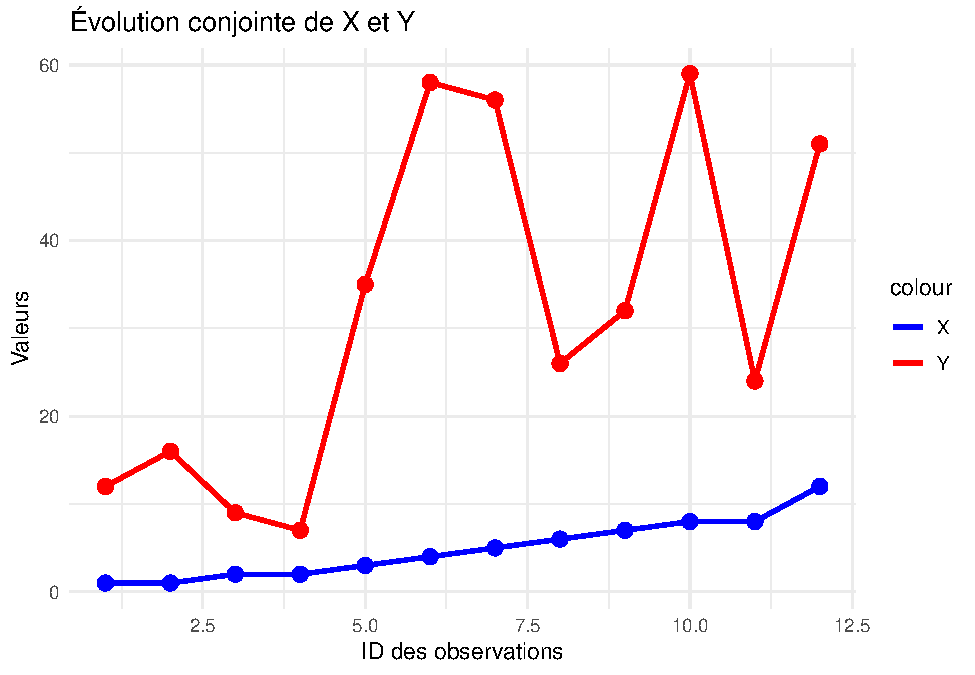
\includegraphics{Stat_non_para_files/figure-latex/unnamed-chunk-59-1.pdf}

On a l'impression que les deux echantillons sont indépendants car X a
une tendance plutôt croissante tandis que Y croit puis décroit de temps
à autre. toutefois, les tendances des deux échantillons sont globalement
croissantes. Voyons les résultats fournis par les tests.

\begin{itemize}
\tightlist
\item
  \textbf{Tests}
\end{itemize}

\begin{Shaded}
\begin{Highlighting}[]
\CommentTok{\# {-}{-}{-}{-}{-}{-}{-}{-}{-}{-}{-}{-}{-}{-}{-}{-}{-}{-}{-}{-}{-}{-}{-}{-}{-}{-}{-}{-}}
\CommentTok{\#  }\AlertTok{TEST}\CommentTok{ INTÉGRÉ DE SPEARMAN ET }\AlertTok{TEST}\CommentTok{ MANUEL}
\CommentTok{\# {-}{-}{-}{-}{-}{-}{-}{-}{-}{-}{-}{-}{-}{-}{-}{-}{-}{-}{-}{-}{-}{-}{-}{-}{-}{-}{-}{-}}
\CommentTok{\# Choisir l\textquotesingle{}alternative en fonction du graphique: "two.sided", "greater", ou "less"}

\NormalTok{alternative\_choice }\OtherTok{\textless{}{-}} \StringTok{"two.sided"} 

\NormalTok{result\_manual }\OtherTok{\textless{}{-}} \FunctionTok{spearman\_test\_manual}\NormalTok{(data}\SpecialCharTok{$}\NormalTok{X, data}\SpecialCharTok{$}\NormalTok{Y, }\AttributeTok{alternative =}\NormalTok{ alternative\_choice)}
\end{Highlighting}
\end{Shaded}

\begin{verbatim}
## Test de Spearman Manuel
## -----------------------
## Type de test    : Bilatéral (dépendance quelconque) 
## Statistique T   : 594.5 
## Statistique Z   : 2.0401 
## Valeur critique : 1.96 
## Règle de décision: |Z| > 1.96 
## p-value         : 0.041344 
## Coefficient ρ   : 0.6184 
## Décision        : Rejeter H0 au seuil 0.05 
## -----------------------
\end{verbatim}

\begin{Shaded}
\begin{Highlighting}[]
\NormalTok{result\_builtin }\OtherTok{\textless{}{-}} \FunctionTok{cor.test}\NormalTok{(data}\SpecialCharTok{$}\NormalTok{X, data}\SpecialCharTok{$}\NormalTok{Y, }\AttributeTok{method =} \StringTok{"spearman"}\NormalTok{, }\AttributeTok{exact =} \ConstantTok{FALSE}\NormalTok{, }
                           \AttributeTok{alternative =}\NormalTok{ alternative\_choice)}


\CommentTok{\# {-}{-}{-}{-}{-}{-}{-}{-}{-}{-}{-}{-}{-}{-}{-}{-}{-}{-}{-}{-}{-}{-}{-}{-}{-}{-}{-}{-}}
\CommentTok{\#  COMPARAISON DES RÉSULTATS}
\CommentTok{\# {-}{-}{-}{-}{-}{-}{-}{-}{-}{-}{-}{-}{-}{-}{-}{-}{-}{-}{-}{-}{-}{-}{-}{-}{-}{-}{-}{-}}

\FunctionTok{cat}\NormalTok{(}\StringTok{"}\SpecialCharTok{\textbackslash{}n}\StringTok{=== Résultats du test intégré ===}\SpecialCharTok{\textbackslash{}n}\StringTok{"}\NormalTok{)}
\end{Highlighting}
\end{Shaded}

\begin{verbatim}
## 
## === Résultats du test intégré ===
\end{verbatim}

\begin{Shaded}
\begin{Highlighting}[]
\FunctionTok{print}\NormalTok{(}\FunctionTok{data.frame}\NormalTok{(}
  \AttributeTok{Coefficient\_rho =}\NormalTok{ result\_builtin}\SpecialCharTok{$}\NormalTok{estimate,}
  \AttributeTok{P\_value =}\NormalTok{ result\_builtin}\SpecialCharTok{$}\NormalTok{p.value,}
\NormalTok{  Méthode }\OtherTok{=}\NormalTok{ result\_builtin}\SpecialCharTok{$}\NormalTok{method}
\NormalTok{))}
\end{Highlighting}
\end{Shaded}

\begin{verbatim}
##     Coefficient_rho    P_value                         Méthode
## rho       0.6151228 0.03326601 Spearman's rank correlation rho
\end{verbatim}

Les deux tests rejettent H0 au seuil 0.05. donc il y a dépendance entre
les deux échantillons au seuil 0.05. Mais si on prend un faible risque
comme 1\%, on ne va plus rejeter H0, donc les 2 échantillons seront
indépendants dans ce cas là, ce qui est en ligne avec l'observation
faite sur le graphique.

\subsubsection{Test de Kendall: cas
apparié}\label{test-de-kendall-cas-appariuxe9}

\begin{itemize}
\tightlist
\item
  \textbf{Données}
\end{itemize}

\begin{Shaded}
\begin{Highlighting}[]
\CommentTok{\# Données du cours}
\NormalTok{x }\OtherTok{\textless{}{-}} \FunctionTok{c}\NormalTok{(}\DecValTok{1}\NormalTok{,}\DecValTok{1}\NormalTok{,}\DecValTok{2}\NormalTok{, }\DecValTok{2}\NormalTok{, }\DecValTok{3}\NormalTok{, }\DecValTok{4}\NormalTok{, }\DecValTok{5}\NormalTok{, }\DecValTok{6}\NormalTok{, }\DecValTok{7}\NormalTok{, }\DecValTok{8}\NormalTok{, }\DecValTok{8}\NormalTok{, }\DecValTok{12}\NormalTok{)}
\NormalTok{y }\OtherTok{\textless{}{-}} \FunctionTok{c}\NormalTok{(}\DecValTok{12}\NormalTok{, }\DecValTok{16}\NormalTok{, }\DecValTok{9}\NormalTok{, }\DecValTok{7}\NormalTok{, }\DecValTok{35}\NormalTok{, }\DecValTok{58}\NormalTok{, }\DecValTok{56}\NormalTok{, }\DecValTok{26}\NormalTok{, }\DecValTok{32}\NormalTok{, }\DecValTok{59}\NormalTok{, }\DecValTok{24}\NormalTok{, }\DecValTok{51}\NormalTok{)}
\end{Highlighting}
\end{Shaded}

\begin{itemize}
\tightlist
\item
  \textbf{Visualisation}
\end{itemize}

\begin{Shaded}
\begin{Highlighting}[]
\CommentTok{\# Génération de l\textquotesingle{}indice i}
\NormalTok{i }\OtherTok{\textless{}{-}} \DecValTok{1}\SpecialCharTok{:}\FunctionTok{length}\NormalTok{(x)}

\CommentTok{\# Tracé des deux courbes}
\FunctionTok{plot}\NormalTok{(i, x, }\AttributeTok{type =} \StringTok{"o"}\NormalTok{, }\AttributeTok{col =} \StringTok{"blue"}\NormalTok{, }\AttributeTok{pch =} \DecValTok{16}\NormalTok{, }\AttributeTok{ylim =} \FunctionTok{range}\NormalTok{(}\FunctionTok{c}\NormalTok{(x, y)),}
     \AttributeTok{xlab =} \StringTok{"Indice (i)"}\NormalTok{, }\AttributeTok{ylab =} \StringTok{"Valeurs"}\NormalTok{, }\AttributeTok{main =} \StringTok{"Évolution de xᵢ et yᵢ"}\NormalTok{)}
\FunctionTok{lines}\NormalTok{(i, y, }\AttributeTok{type =} \StringTok{"o"}\NormalTok{, }\AttributeTok{col =} \StringTok{"red"}\NormalTok{, }\AttributeTok{pch =} \DecValTok{17}\NormalTok{, }\AttributeTok{lty =} \DecValTok{2}\NormalTok{)}

\CommentTok{\# Légende}
\FunctionTok{legend}\NormalTok{(}\StringTok{"topright"}\NormalTok{, }\AttributeTok{legend =} \FunctionTok{c}\NormalTok{(}\StringTok{"xᵢ"}\NormalTok{, }\StringTok{"yᵢ"}\NormalTok{),}
       \AttributeTok{col =} \FunctionTok{c}\NormalTok{(}\StringTok{"blue"}\NormalTok{, }\StringTok{"red"}\NormalTok{), }\AttributeTok{pch =} \FunctionTok{c}\NormalTok{(}\DecValTok{16}\NormalTok{, }\DecValTok{17}\NormalTok{), }\AttributeTok{lty =} \FunctionTok{c}\NormalTok{(}\DecValTok{1}\NormalTok{, }\DecValTok{2}\NormalTok{))}
\FunctionTok{grid}\NormalTok{()}
\end{Highlighting}
\end{Shaded}

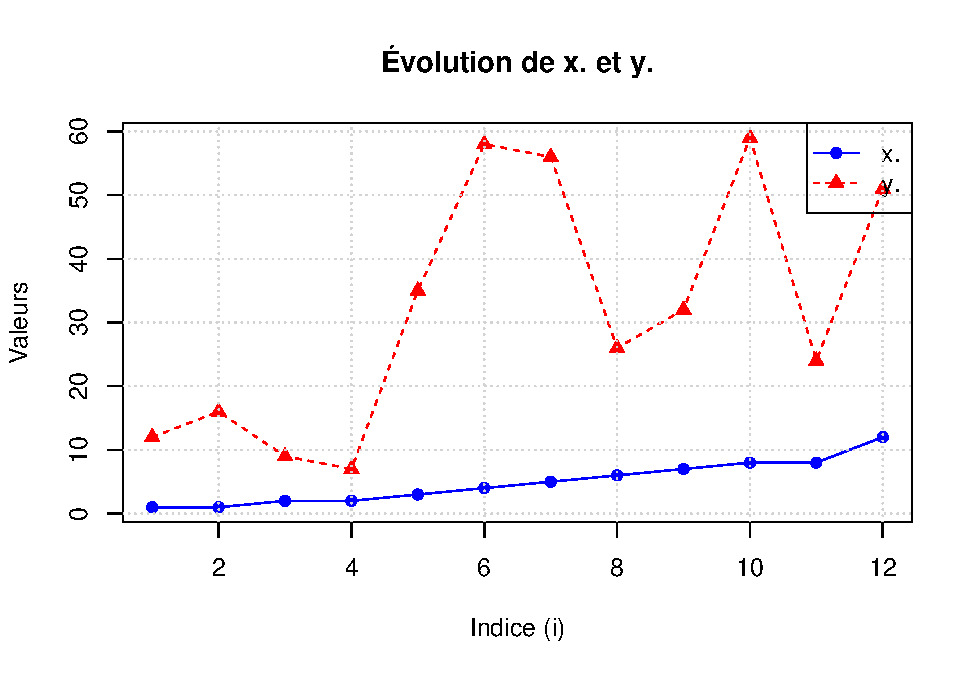
\includegraphics{Stat_non_para_files/figure-latex/unnamed-chunk-62-1.pdf}

Le principe est le même que dans le cas d'un échantillon. On regarde le
nombre de paires concordantes entre (Xi,Yi) et (Xj,Yj).

\begin{itemize}
\tightlist
\item
  \textbf{Hypothèses :}
\end{itemize}

\[
\begin{cases} 
H_0 : \text{Les données sont iid} \\ 
H_1 : \text{les données ne sont pas iid}
\end{cases}
\]

\begin{itemize}
\item
  \textbf{La statistique de Kendal}

  \begin{itemize}
  \tightlist
  \item
    \textbf{Calcul de Q}
  \end{itemize}
\end{itemize}

Il y'a concordante entre ces deux couples si :

\((Xi −Xj)(Yj −Yi) > 0\) i.e \(Xj > Xi\) et \(Yj > Yi\) ou \(Xj < Xi\)
et \(Yj < Yi\)

Donc on a:

\[
Q = \sum_{i=1}^{n-1} \sum_{j=i+1}^{n} \mathbb{1}\left[(x_j - x_i)(y_j - y_i) > 0\right]
\]

\begin{Shaded}
\begin{Highlighting}[]
\NormalTok{QKendall }\OtherTok{\textless{}{-}} \ControlFlowTok{function}\NormalTok{(x, y) \{}
\NormalTok{  n }\OtherTok{\textless{}{-}} \FunctionTok{length}\NormalTok{(x)}
\NormalTok{  count }\OtherTok{\textless{}{-}} \DecValTok{0}
  \ControlFlowTok{for}\NormalTok{ (i }\ControlFlowTok{in} \DecValTok{1}\SpecialCharTok{:}\NormalTok{(n}\DecValTok{{-}1}\NormalTok{)) \{}
    \ControlFlowTok{for}\NormalTok{ (j }\ControlFlowTok{in}\NormalTok{ (i}\SpecialCharTok{+}\DecValTok{1}\NormalTok{)}\SpecialCharTok{:}\NormalTok{n) \{}
      \ControlFlowTok{if}\NormalTok{ ((x[j] }\SpecialCharTok{{-}}\NormalTok{ x[i]) }\SpecialCharTok{*}\NormalTok{ (y[j] }\SpecialCharTok{{-}}\NormalTok{ y[i]) }\SpecialCharTok{\textgreater{}} \DecValTok{0}\NormalTok{) \{}
\NormalTok{        count }\OtherTok{\textless{}{-}}\NormalTok{ count }\SpecialCharTok{+} \DecValTok{1}
\NormalTok{      \}}
\NormalTok{    \}}
\NormalTok{  \}}
  \FunctionTok{return}\NormalTok{(count)}
\NormalTok{\}}
\FunctionTok{print}\NormalTok{(}\StringTok{"le Q Kendall est : "}\NormalTok{)}
\end{Highlighting}
\end{Shaded}

\begin{verbatim}
## [1] "le Q Kendall est : "
\end{verbatim}

\begin{Shaded}
\begin{Highlighting}[]
\FunctionTok{QKendall}\NormalTok{(x,y)}
\end{Highlighting}
\end{Shaded}

\begin{verbatim}
## [1] 44
\end{verbatim}

\begin{itemize}
\tightlist
\item
  \textbf{Calcul du \(\tau\)}
\end{itemize}

On pose: \(\tau = 1 - \frac{4Q}{n(n-1)}\)

\begin{Shaded}
\begin{Highlighting}[]
\NormalTok{StatTest }\OtherTok{\textless{}{-}} \ControlFlowTok{function}\NormalTok{(x, y) \{}
\NormalTok{  n }\OtherTok{\textless{}{-}} \FunctionTok{length}\NormalTok{(x)}
\NormalTok{  Q }\OtherTok{\textless{}{-}} \FunctionTok{QKendall}\NormalTok{(x, y)}
\NormalTok{  tau }\OtherTok{\textless{}{-}} \DecValTok{1} \SpecialCharTok{{-}}\NormalTok{ (}\DecValTok{4} \SpecialCharTok{*}\NormalTok{ Q) }\SpecialCharTok{/}\NormalTok{ (n }\SpecialCharTok{*}\NormalTok{ (n }\SpecialCharTok{{-}} \DecValTok{1}\NormalTok{))}
  \FunctionTok{return}\NormalTok{(tau)}
\NormalTok{\}}

\NormalTok{tau }\OtherTok{\textless{}{-}} \FunctionTok{StatTest}\NormalTok{(x, y)}
\NormalTok{tau}
\end{Highlighting}
\end{Shaded}

\begin{verbatim}
## [1] -0.3333333
\end{verbatim}

Pour n assez grand, la valeur Z observée se calcule comme suit :

\[
Z_{obs} = \frac{\tau - \mathbb{E}(\tau)}{\sqrt{Var(\tau)}}
\]

Avec:

\[
E(\tau) = 1 - \frac{4n(n-1)}{4n(n-1)} = 0
\]

\[
V(\tau) = \frac{2(2n+5)}{9n(n-1)}
\]

\begin{Shaded}
\begin{Highlighting}[]
\NormalTok{Zobs }\OtherTok{\textless{}{-}} \ControlFlowTok{function}\NormalTok{(x, y) \{}
\NormalTok{  n }\OtherTok{\textless{}{-}} \FunctionTok{length}\NormalTok{(x)}
\NormalTok{  tau }\OtherTok{\textless{}{-}} \FunctionTok{StatTest}\NormalTok{(x, y)}
\NormalTok{  variance\_tau }\OtherTok{\textless{}{-}}\NormalTok{ (}\DecValTok{2} \SpecialCharTok{*}\NormalTok{ (}\DecValTok{2} \SpecialCharTok{*}\NormalTok{ n }\SpecialCharTok{+} \DecValTok{5}\NormalTok{)) }\SpecialCharTok{/}\NormalTok{ (}\DecValTok{9} \SpecialCharTok{*}\NormalTok{ n }\SpecialCharTok{*}\NormalTok{ (n }\SpecialCharTok{{-}} \DecValTok{1}\NormalTok{))}
\NormalTok{  z }\OtherTok{\textless{}{-}}\NormalTok{ tau }\SpecialCharTok{/} \FunctionTok{sqrt}\NormalTok{(variance\_tau)}
  \FunctionTok{return}\NormalTok{(z)}
\NormalTok{\}}

\NormalTok{z\_obs }\OtherTok{\textless{}{-}} \FunctionTok{Zobs}\NormalTok{(x, y)}
\NormalTok{z\_obs}
\end{Highlighting}
\end{Shaded}

\begin{verbatim}
## [1] -1.508596
\end{verbatim}

\begin{itemize}
\tightlist
\item
  \textbf{Région critique et prise de décision}
\end{itemize}

Soit un seuil de signification \(\alpha\) donné. La statistique de test
\(Z_{\text{obs}}\) suit approximativement une loi normale
\(\mathcal{N}(0,1)\) sous l'hypothèse nulle \((H_0)\).

\paragraph{Test bilatéral}\label{test-bilatuxe9ral}

\[
\text{Rejeter } H_0 \text{ si } |Z_{\text{obs}}| > z_{1 - \alpha/2}
\]

\begin{Shaded}
\begin{Highlighting}[]
\NormalTok{Kendall\_Test }\OtherTok{\textless{}{-}} \ControlFlowTok{function}\NormalTok{(risque, x, y) \{}
\NormalTok{  zobs }\OtherTok{\textless{}{-}} \FunctionTok{Zobs}\NormalTok{(x, y)}
\NormalTok{  seuil }\OtherTok{\textless{}{-}} \FunctionTok{qnorm}\NormalTok{(}\DecValTok{1} \SpecialCharTok{{-}}\NormalTok{ risque }\SpecialCharTok{/} \DecValTok{2}\NormalTok{)  }\CommentTok{\# Bilatéral}

  \FunctionTok{cat}\NormalTok{(}\StringTok{"Z observé ="}\NormalTok{, }\FunctionTok{round}\NormalTok{(zobs, }\DecValTok{3}\NormalTok{), }\StringTok{"}\SpecialCharTok{\textbackslash{}n}\StringTok{"}\NormalTok{)}
  \FunctionTok{cat}\NormalTok{(}\StringTok{"Seuil critique (bilatéral) ="}\NormalTok{, }\FunctionTok{round}\NormalTok{(seuil, }\DecValTok{3}\NormalTok{), }\StringTok{"}\SpecialCharTok{\textbackslash{}n}\StringTok{"}\NormalTok{)}
  
  \ControlFlowTok{if}\NormalTok{ (}\FunctionTok{abs}\NormalTok{(zobs) }\SpecialCharTok{\textgreater{}}\NormalTok{ seuil) \{}
    \FunctionTok{print}\NormalTok{(}\StringTok{"On rejette H0 : Il existe une dépendance significative entre X et Y."}\NormalTok{)}
\NormalTok{  \} }\ControlFlowTok{else}\NormalTok{ \{}
    \FunctionTok{print}\NormalTok{(}\StringTok{"On ne rejette pas H0 : Pas de dépendance significative entre X et Y."}\NormalTok{)}
\NormalTok{  \}}
\NormalTok{\}}
\FunctionTok{Kendall\_Test}\NormalTok{(}\FloatTok{0.1}\NormalTok{, x, y)}
\end{Highlighting}
\end{Shaded}

\begin{verbatim}
## Z observé = -1.509 
## Seuil critique (bilatéral) = 1.645 
## [1] "On ne rejette pas H0 : Pas de dépendance significative entre X et Y."
\end{verbatim}

Pour n faible alors :

\begin{itemize}
\tightlist
\item
  \textbf{Définition de la statistique S}
\end{itemize}

On a : - \(Q\) : nombre de paires \textbf{concordantes} - \(Q'\) :
nombre de paires \textbf{discordantes}

\begin{Shaded}
\begin{Highlighting}[]
\CommentTok{\# Fonction qui retourne les valeurs de Q (concordant), Q\textquotesingle{} (discordant), et S}
\NormalTok{SKendall }\OtherTok{\textless{}{-}} \ControlFlowTok{function}\NormalTok{(x, y) \{}
\NormalTok{  n }\OtherTok{\textless{}{-}} \FunctionTok{length}\NormalTok{(x)}
\NormalTok{  Q\_concordant }\OtherTok{\textless{}{-}} \DecValTok{0}
\NormalTok{  Q\_discordant }\OtherTok{\textless{}{-}} \DecValTok{0}
  
  \ControlFlowTok{for}\NormalTok{ (i }\ControlFlowTok{in} \DecValTok{1}\SpecialCharTok{:}\NormalTok{(n }\SpecialCharTok{{-}} \DecValTok{1}\NormalTok{)) \{}
    \ControlFlowTok{for}\NormalTok{ (j }\ControlFlowTok{in}\NormalTok{ (i }\SpecialCharTok{+} \DecValTok{1}\NormalTok{)}\SpecialCharTok{:}\NormalTok{n) \{}
\NormalTok{      produit }\OtherTok{\textless{}{-}}\NormalTok{ (x[j] }\SpecialCharTok{{-}}\NormalTok{ x[i]) }\SpecialCharTok{*}\NormalTok{ (y[j] }\SpecialCharTok{{-}}\NormalTok{ y[i])}
      
      \ControlFlowTok{if}\NormalTok{ (produit }\SpecialCharTok{\textgreater{}} \DecValTok{0}\NormalTok{) \{}
\NormalTok{        Q\_concordant }\OtherTok{\textless{}{-}}\NormalTok{ Q\_concordant }\SpecialCharTok{+} \DecValTok{1}
\NormalTok{      \} }\ControlFlowTok{else} \ControlFlowTok{if}\NormalTok{ (produit }\SpecialCharTok{\textless{}} \DecValTok{0}\NormalTok{) \{}
\NormalTok{        Q\_discordant }\OtherTok{\textless{}{-}}\NormalTok{ Q\_discordant }\SpecialCharTok{+} \DecValTok{1}
\NormalTok{      \}}
      \CommentTok{\# si produit == 0 → égalité → on ignore}
\NormalTok{    \}}
\NormalTok{  \}}
  
\NormalTok{  S }\OtherTok{\textless{}{-}}\NormalTok{ Q\_discordant }\SpecialCharTok{{-}}\NormalTok{ Q\_concordant}
  
  \FunctionTok{return}\NormalTok{(}\FunctionTok{list}\NormalTok{(}
    \AttributeTok{Q\_concordant =}\NormalTok{ Q\_concordant,}
    \AttributeTok{Q\_discordant =}\NormalTok{ Q\_discordant,}
    \AttributeTok{S =}\NormalTok{ S}
\NormalTok{  ))}
\NormalTok{\}}
\NormalTok{result}\OtherTok{=}\FunctionTok{SKendall}\NormalTok{(x,y)}

\FunctionTok{print}\NormalTok{(}\FunctionTok{paste}\NormalTok{(}\StringTok{"Q concordant ="}\NormalTok{, result}\SpecialCharTok{$}\NormalTok{Q\_concordant))}
\end{Highlighting}
\end{Shaded}

\begin{verbatim}
## [1] "Q concordant = 44"
\end{verbatim}

\begin{Shaded}
\begin{Highlighting}[]
\FunctionTok{print}\NormalTok{(}\FunctionTok{paste}\NormalTok{(}\StringTok{"Q discordant ="}\NormalTok{, result}\SpecialCharTok{$}\NormalTok{Q\_discordant))}
\end{Highlighting}
\end{Shaded}

\begin{verbatim}
## [1] "Q discordant = 19"
\end{verbatim}

\begin{Shaded}
\begin{Highlighting}[]
\FunctionTok{print}\NormalTok{(}\FunctionTok{paste}\NormalTok{(}\StringTok{"S ="}\NormalTok{, result}\SpecialCharTok{$}\NormalTok{S))}
\end{Highlighting}
\end{Shaded}

\begin{verbatim}
## [1] "S = -25"
\end{verbatim}

\begin{itemize}
\tightlist
\item
  \textbf{Test bilatéral} : \$\text{Rejeter } \quad H\_0
  \quad \text{ si } \textbar S\textbar{} \textgreater{} s \$
\end{itemize}

D'après la table de Kendall S= 28 donc on ne rejette pas \(H_0\).

\paragraph{Avec la fonction intégrée
R}\label{avec-la-fonction-intuxe9gruxe9e-r}

\begin{Shaded}
\begin{Highlighting}[]
\FunctionTok{cor.test}\NormalTok{(x, y, }\AttributeTok{method =} \StringTok{"kendall"}\NormalTok{, }\AttributeTok{exact =} \ConstantTok{TRUE}\NormalTok{)}
\end{Highlighting}
\end{Shaded}

\begin{verbatim}
## 
##  Kendall's rank correlation tau
## 
## data:  x and y
## z = 1.7265, p-value = 0.08425
## alternative hypothesis: true tau is not equal to 0
## sample estimates:
##       tau 
## 0.3877018
\end{verbatim}

\subsection{Tests d'alternative de
position}\label{tests-dalternative-de-position}

\subsubsection{Test de Wilcoxon}\label{test-de-wilcoxon}

Le test de Wilcoxon permet de comparer la position (typiquement la
médiane) de deux échantillons pour évaluer s'ils proviennent de
populations ayant le même paramètre de position.

Hypothèse nulle \((H_0)\) : Les deux groupes ont la même distribution,
donc le même paramètre de position (médiane).

On considère l'échantillon fusionné
\((X_1, X_2, \dots, X_n, Y_1, Y_2, \dots, Y_m) = (X_1, X_2, \dots, X_{n+m})\)
et on note par \(R_i\) le rang de \(X_i\) dans l'échantillon fusionné.

La statistique de Wilcoxon est : \(\quad W_n = \sum_{i=1}^{n} R_i\)

\[
\textbf{La région critique est :} \quad
W =
\begin{cases}
W_n < c & \text{pour } H_1 : \theta > 0 \quad \text{alors } Y \gg X \\
W_n > c & \text{pour } H_1 : \theta < 0 \quad \text{alors } X \gg Y \\
W_n < c \text{ ou } W_n > c & \text{pour } H_1 : \theta \neq 0
\end{cases}
\]

\[
\begin{aligned}
&\text{Sous } H_0, W_n \text{ est symétrique autour de sa moyenne.} \\
&\mathbb{E}(W_n) = \sum \mathbb{E}(R_i) = n \cdot \mathbb{E}(R_i) = n \cdot \frac{n + m + 1}{2} \\[10pt]
&\text{On remarque également :} \quad \mathbb{V}(W_n) = \frac{nm(n + m + 1)}{12} \\[10pt]
&\text{Les valeurs extrêmes de } W_n \text{ sont :} \\
&\textbf{a. } \text{Si tous les } X_i < Y_i \Rightarrow W_n = 1 + 2 + \cdots + n = \frac{n(n + 1)}{2} \\
&\textbf{b. } \text{Si tous les } X_i > Y_i \Rightarrow W_n = (m + 1) + (m + 2) + \cdots + (m + n) \\
&\phantom{\textbf{b. }} \Rightarrow W_n = nm + \frac{n(n + 1)}{2} \\[10pt]
&\text{Pour des échantillons de petite taille, on utilise la table de Wilcoxon.} \\
&\text{Pour des grands échantillons, on utilise l’approximation :} \\
&\frac{W_n - \mathbb{E}(W_n)}{\sqrt{\mathbb{V}(W_n)}} \longrightarrow \mathcal{N}(0, 1)
\end{aligned}
\]

\begin{itemize}
\tightlist
\item
  \textbf{Simulation}
\end{itemize}

\begin{Shaded}
\begin{Highlighting}[]
\FunctionTok{require}\NormalTok{(graphics)}
\FunctionTok{par}\NormalTok{(}\AttributeTok{mfrow =} \FunctionTok{c}\NormalTok{(}\DecValTok{2}\NormalTok{,}\DecValTok{2}\NormalTok{))}
\ControlFlowTok{for}\NormalTok{(n }\ControlFlowTok{in} \FunctionTok{c}\NormalTok{(}\DecValTok{4}\SpecialCharTok{:}\DecValTok{5}\NormalTok{,}\DecValTok{10}\NormalTok{,}\DecValTok{40}\NormalTok{)) \{}
\NormalTok{  x }\OtherTok{\textless{}{-}} \FunctionTok{seq}\NormalTok{(}\DecValTok{0}\NormalTok{, n}\SpecialCharTok{*}\NormalTok{(n}\SpecialCharTok{+}\DecValTok{1}\NormalTok{)}\SpecialCharTok{/}\DecValTok{2}\NormalTok{, }\AttributeTok{length.out =} \DecValTok{501}\NormalTok{)}
  \FunctionTok{plot}\NormalTok{(x, }\FunctionTok{dsignrank}\NormalTok{(x, }\AttributeTok{n =}\NormalTok{ n), }\AttributeTok{type =} \StringTok{"l"}\NormalTok{,}
       \AttributeTok{main =} \FunctionTok{paste0}\NormalTok{(}\StringTok{"dsignrank(x, n = "}\NormalTok{, n, }\StringTok{")"}\NormalTok{))}
\NormalTok{\}}
\end{Highlighting}
\end{Shaded}

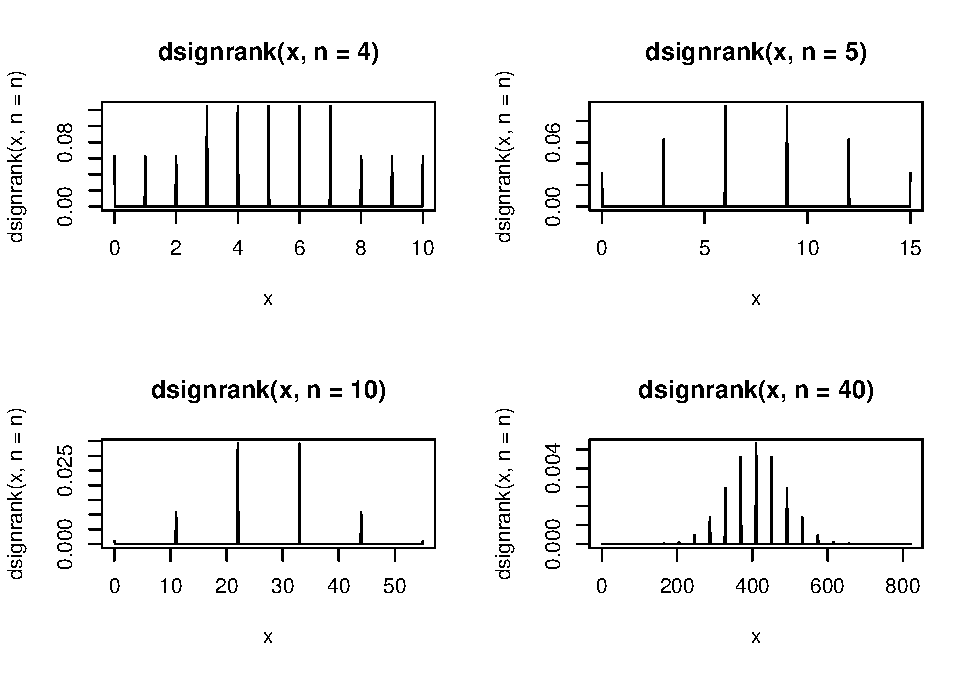
\includegraphics{Stat_non_para_files/figure-latex/unnamed-chunk-69-1.pdf}

\begin{itemize}
\tightlist
\item
  \textbf{Données}
\end{itemize}

\begin{Shaded}
\begin{Highlighting}[]
\CommentTok{\# Simulation de deux échantillons indépendants}
\NormalTok{x }\OtherTok{\textless{}{-}} \FunctionTok{c}\NormalTok{(}\DecValTok{21}\NormalTok{,}\DecValTok{22}\NormalTok{, }\DecValTok{14}\NormalTok{, }\DecValTok{25}\NormalTok{,}\DecValTok{15}\NormalTok{,}\DecValTok{17}\NormalTok{)   }\CommentTok{\# Échantillon X}
\NormalTok{y }\OtherTok{\textless{}{-}} \FunctionTok{c}\NormalTok{(}\DecValTok{18}\NormalTok{, }\DecValTok{14}\NormalTok{, }\DecValTok{21}\NormalTok{,}\DecValTok{14}\NormalTok{,}\DecValTok{24}\NormalTok{,}\DecValTok{26}\NormalTok{,}\DecValTok{19}\NormalTok{,}\DecValTok{20}\NormalTok{)   }\CommentTok{\# Échantillon Y}
\NormalTok{n }\OtherTok{\textless{}{-}} \FunctionTok{length}\NormalTok{(x)}
\NormalTok{m }\OtherTok{\textless{}{-}} \FunctionTok{length}\NormalTok{(y)}
\NormalTok{N }\OtherTok{\textless{}{-}}\NormalTok{ n}\SpecialCharTok{+}\NormalTok{m}
\end{Highlighting}
\end{Shaded}

\begin{Shaded}
\begin{Highlighting}[]
\NormalTok{i }\OtherTok{\textless{}{-}} \DecValTok{1}\SpecialCharTok{:}\NormalTok{n}
\FunctionTok{plot}\NormalTok{(i, x, }\AttributeTok{col =} \StringTok{"blue"}\NormalTok{ )}
\FunctionTok{lines}\NormalTok{(x, }\AttributeTok{col =} \StringTok{"blue"}\NormalTok{ )}
\FunctionTok{lines}\NormalTok{(y, }\AttributeTok{col =} \StringTok{"red"}\NormalTok{)}
\end{Highlighting}
\end{Shaded}

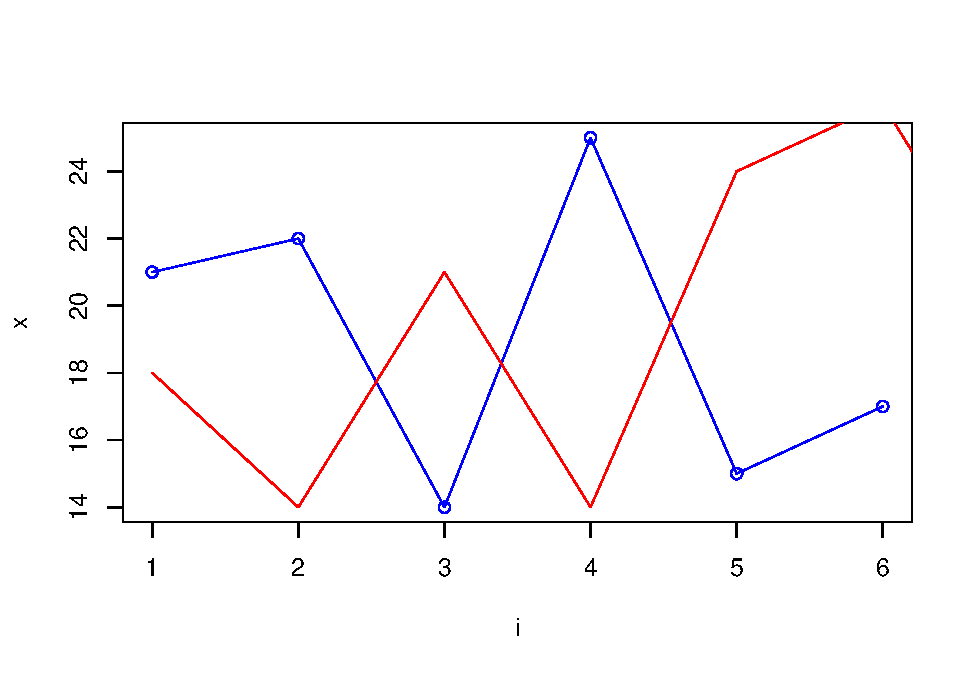
\includegraphics{Stat_non_para_files/figure-latex/unnamed-chunk-71-1.pdf}

\begin{itemize}
\tightlist
\item
  \textbf{Visualisation : Fonctions de répartition empiriques}
\end{itemize}

\begin{Shaded}
\begin{Highlighting}[]
\FunctionTok{plot}\NormalTok{(}\FunctionTok{ecdf}\NormalTok{(x), }\AttributeTok{main =} \StringTok{"Fonctions de Répartition Empiriques"}\NormalTok{, }\AttributeTok{xlab =} \StringTok{"Valeurs"}\NormalTok{, }
     \AttributeTok{ylab =} \StringTok{"F(x)"}\NormalTok{, }\AttributeTok{col =} \StringTok{"blue"}\NormalTok{, }\AttributeTok{lwd =} \DecValTok{2}\NormalTok{)}
\FunctionTok{lines}\NormalTok{(}\FunctionTok{ecdf}\NormalTok{(y), }\AttributeTok{col =} \StringTok{"red"}\NormalTok{, }\AttributeTok{lwd =} \DecValTok{2}\NormalTok{)}
\FunctionTok{legend}\NormalTok{(}\StringTok{"bottomright"}\NormalTok{, }\AttributeTok{legend =} \FunctionTok{c}\NormalTok{(}\StringTok{"X"}\NormalTok{, }\StringTok{"Y"}\NormalTok{), }\AttributeTok{col =} \FunctionTok{c}\NormalTok{(}\StringTok{"blue"}\NormalTok{, }\StringTok{"red"}\NormalTok{), }\AttributeTok{lwd =} \DecValTok{2}\NormalTok{)}
\end{Highlighting}
\end{Shaded}

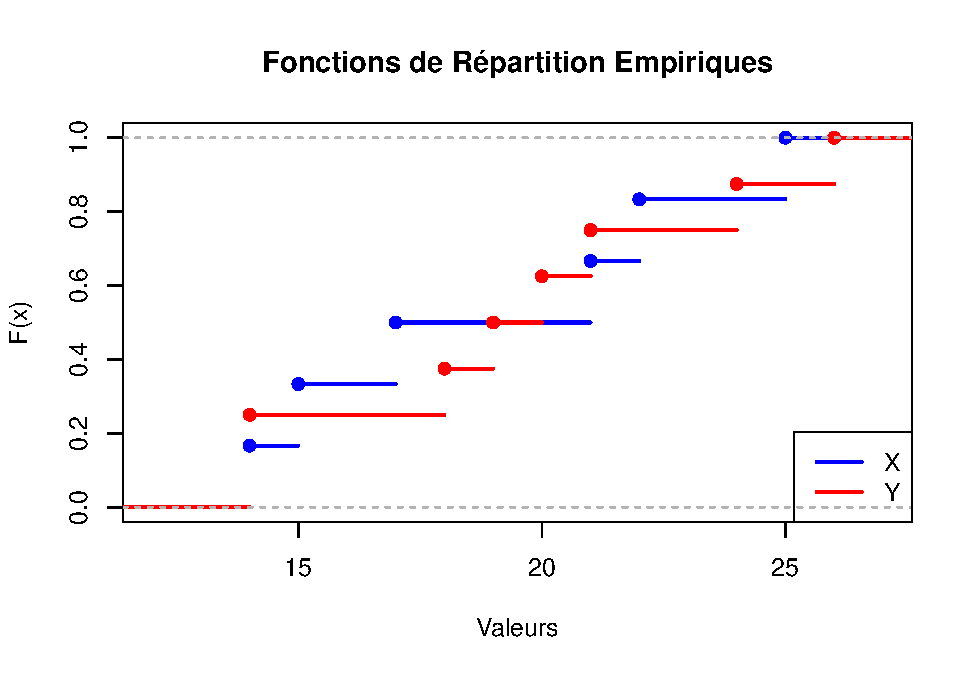
\includegraphics{Stat_non_para_files/figure-latex/unnamed-chunk-72-1.pdf}

\begin{Shaded}
\begin{Highlighting}[]
\CommentTok{\# Estimation de la densité avec densité par noyau}
\NormalTok{d\_x }\OtherTok{\textless{}{-}} \FunctionTok{density}\NormalTok{(x)}
\NormalTok{d\_y }\OtherTok{\textless{}{-}} \FunctionTok{density}\NormalTok{(y)}

\CommentTok{\# Fonction de répartition obtenue par intégration numérique}
\NormalTok{Fx }\OtherTok{\textless{}{-}} \FunctionTok{approxfun}\NormalTok{(d\_x}\SpecialCharTok{$}\NormalTok{x, }\FunctionTok{cumsum}\NormalTok{(d\_x}\SpecialCharTok{$}\NormalTok{y) }\SpecialCharTok{/} \FunctionTok{sum}\NormalTok{(d\_x}\SpecialCharTok{$}\NormalTok{y))}
\NormalTok{Fy }\OtherTok{\textless{}{-}} \FunctionTok{approxfun}\NormalTok{(d\_y}\SpecialCharTok{$}\NormalTok{x, }\FunctionTok{cumsum}\NormalTok{(d\_y}\SpecialCharTok{$}\NormalTok{y) }\SpecialCharTok{/} \FunctionTok{sum}\NormalTok{(d\_y}\SpecialCharTok{$}\NormalTok{y))}

\CommentTok{\# Séquence de valeurs communes pour comparer}
\NormalTok{x\_vals }\OtherTok{\textless{}{-}} \FunctionTok{seq}\NormalTok{(}\FunctionTok{min}\NormalTok{(}\FunctionTok{c}\NormalTok{(x, y)) }\SpecialCharTok{{-}} \DecValTok{1}\NormalTok{, }\FunctionTok{max}\NormalTok{(}\FunctionTok{c}\NormalTok{(x, y)) }\SpecialCharTok{+} \DecValTok{1}\NormalTok{, }\AttributeTok{length.out =} \DecValTok{500}\NormalTok{)}

\CommentTok{\# Tracer les courbes lissées}
\FunctionTok{plot}\NormalTok{(x\_vals, }\FunctionTok{Fx}\NormalTok{(x\_vals), }\AttributeTok{type =} \StringTok{"l"}\NormalTok{, }\AttributeTok{col =} \StringTok{"blue"}\NormalTok{, }\AttributeTok{lwd =} \DecValTok{2}\NormalTok{,}
     \AttributeTok{xlab =} \StringTok{"Valeurs"}\NormalTok{, }\AttributeTok{ylab =} \StringTok{"F(x)"}\NormalTok{, }\AttributeTok{main =} \StringTok{"Fonctions de Répartition Lissées"}\NormalTok{)}
\FunctionTok{lines}\NormalTok{(x\_vals, }\FunctionTok{Fy}\NormalTok{(x\_vals), }\AttributeTok{col =} \StringTok{"red"}\NormalTok{, }\AttributeTok{lwd =} \DecValTok{2}\NormalTok{)}
\FunctionTok{legend}\NormalTok{(}\StringTok{"bottomright"}\NormalTok{, }\AttributeTok{legend =} \FunctionTok{c}\NormalTok{(}\StringTok{"X"}\NormalTok{, }\StringTok{"Y"}\NormalTok{), }\AttributeTok{col =} \FunctionTok{c}\NormalTok{(}\StringTok{"blue"}\NormalTok{, }\StringTok{"red"}\NormalTok{), }\AttributeTok{lwd =} \DecValTok{2}\NormalTok{)}
\end{Highlighting}
\end{Shaded}

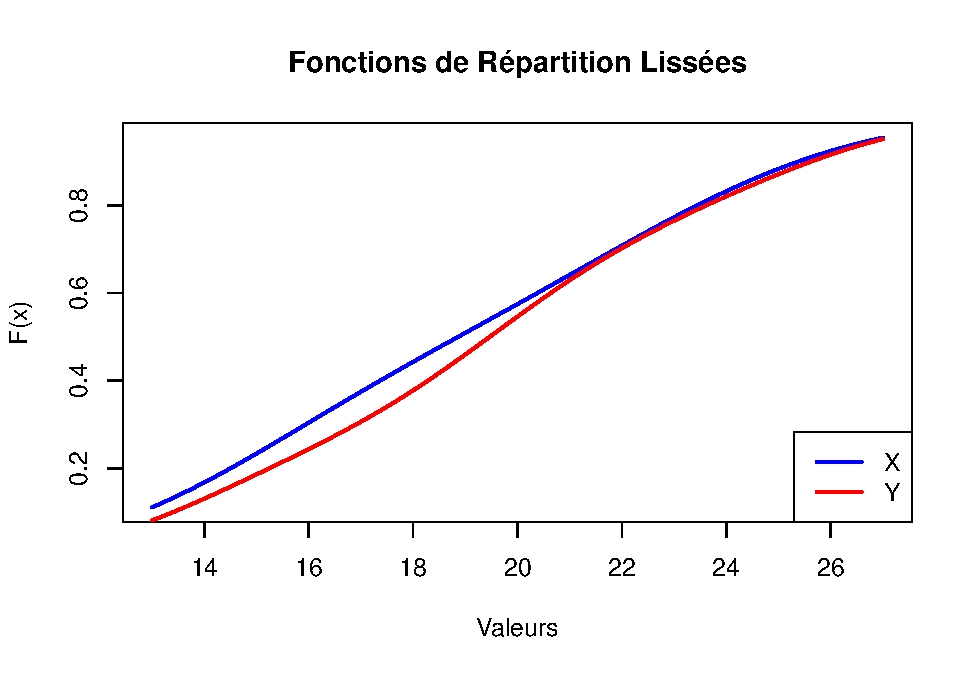
\includegraphics{Stat_non_para_files/figure-latex/unnamed-chunk-73-1.pdf}

\begin{itemize}
\tightlist
\item
  \textbf{Calcul de la statistique Wn}
\end{itemize}

\begin{Shaded}
\begin{Highlighting}[]
\CommentTok{\# Échantillon combiné}
\NormalTok{data\_combined }\OtherTok{\textless{}{-}} \FunctionTok{c}\NormalTok{(x, y)}

\NormalTok{rangs }\OtherTok{\textless{}{-}} \FunctionTok{rank}\NormalTok{(data\_combined, }\AttributeTok{ties.method =}\StringTok{"average"}\NormalTok{)}
\NormalTok{rangs}
\end{Highlighting}
\end{Shaded}

\begin{verbatim}
##  [1]  9.5 11.0  2.0 13.0  4.0  5.0  6.0  2.0  9.5  2.0 12.0 14.0  7.0  8.0
\end{verbatim}

\begin{Shaded}
\begin{Highlighting}[]
\FunctionTok{print}\NormalTok{(}\StringTok{""}\NormalTok{)}
\end{Highlighting}
\end{Shaded}

\begin{verbatim}
## [1] ""
\end{verbatim}

\begin{Shaded}
\begin{Highlighting}[]
\CommentTok{\# Attribution des rangs à X}
\NormalTok{rangs\_x }\OtherTok{\textless{}{-}}\NormalTok{ rangs[}\DecValTok{1}\SpecialCharTok{:}\NormalTok{n]}
\NormalTok{rangs\_x}
\end{Highlighting}
\end{Shaded}

\begin{verbatim}
## [1]  9.5 11.0  2.0 13.0  4.0  5.0
\end{verbatim}

\begin{Shaded}
\begin{Highlighting}[]
\FunctionTok{print}\NormalTok{(}\StringTok{""}\NormalTok{)}
\end{Highlighting}
\end{Shaded}

\begin{verbatim}
## [1] ""
\end{verbatim}

\begin{Shaded}
\begin{Highlighting}[]
\CommentTok{\# Attribution des rangs à X}
\NormalTok{k}\OtherTok{=}\NormalTok{n}\SpecialCharTok{+}\DecValTok{1}
\NormalTok{rangs\_y }\OtherTok{\textless{}{-}}\NormalTok{ rangs[k}\SpecialCharTok{:}\NormalTok{N]}
\NormalTok{rangs\_y}
\end{Highlighting}
\end{Shaded}

\begin{verbatim}
## [1]  6.0  2.0  9.5  2.0 12.0 14.0  7.0  8.0
\end{verbatim}

\begin{Shaded}
\begin{Highlighting}[]
\CommentTok{\# Statistique de Wilcoxon Wn}
\NormalTok{Wn }\OtherTok{\textless{}{-}} \FunctionTok{sum}\NormalTok{(rangs\_x)}
\NormalTok{Wn}
\end{Highlighting}
\end{Shaded}

\begin{verbatim}
## [1] 44.5
\end{verbatim}

\begin{Shaded}
\begin{Highlighting}[]
\CommentTok{\# somme des rangs de y}
\NormalTok{Wy }\OtherTok{\textless{}{-}} \FunctionTok{sum}\NormalTok{(rangs\_y)}
\NormalTok{Wy}
\end{Highlighting}
\end{Shaded}

\begin{verbatim}
## [1] 60.5
\end{verbatim}

\begin{itemize}
\tightlist
\item
  \textbf{Valeur critique au seuil de 5}
\end{itemize}

La fonction \emph{qwilcox} est développé pour la statistique de test de
Wilcoxon Mann-Withney définie par :

\[
\quad U_n = W_n - n(n+1)/2
\]

Donc pour avoir le seuil critique correspondant à la statistique Wn, il
faut ajouter le terme n(n+1)/2

\begin{Shaded}
\begin{Highlighting}[]
\NormalTok{seuil }\OtherTok{\textless{}{-}} \FunctionTok{qwilcox}\NormalTok{(}\AttributeTok{p =} \FloatTok{0.05}\NormalTok{, n, m, }\AttributeTok{lower.tail =}\NormalTok{F) }\SpecialCharTok{+}\NormalTok{ n}\SpecialCharTok{*}\NormalTok{(n}\SpecialCharTok{+}\DecValTok{1}\NormalTok{)}\SpecialCharTok{/}\DecValTok{2}
\NormalTok{seuil}
\end{Highlighting}
\end{Shaded}

\begin{verbatim}
## [1] 58
\end{verbatim}

\begin{itemize}
\tightlist
\item
  \textbf{Prise de décision}
\end{itemize}

\begin{Shaded}
\begin{Highlighting}[]
\CommentTok{\# Test pour H1: X \textgreater{}\textgreater{} Y}
\ControlFlowTok{if}\NormalTok{ (Wn }\SpecialCharTok{\textgreater{}}\NormalTok{ seuil) \{}
  \FunctionTok{cat}\NormalTok{(}\StringTok{"→ Décision : H0 est rejetée au seuil de 5\% — alors X  domine Y.}\SpecialCharTok{\textbackslash{}n}\StringTok{"}\NormalTok{)}
\NormalTok{\} }\ControlFlowTok{else}\NormalTok{ \{}
  \FunctionTok{cat}\NormalTok{(}\StringTok{"→ Décision : H0 n\textquotesingle{}est pas rejetée — aucune dominance significative de X sur Y.}\SpecialCharTok{\textbackslash{}n}\StringTok{"}\NormalTok{)}
\NormalTok{\}}
\end{Highlighting}
\end{Shaded}

\begin{verbatim}
## → Décision : H0 n'est pas rejetée — aucune dominance significative de X sur Y.
\end{verbatim}

\subsubsection{Test de wilcoxon disponible sur
R}\label{test-de-wilcoxon-disponible-sur-r}

\begin{itemize}
\tightlist
\item
  \textbf{Comparaison}
\end{itemize}

\begin{Shaded}
\begin{Highlighting}[]
\CommentTok{\# Test de Wilcoxon pour H1: X \textgreater{}\textgreater{} Y}
\FunctionTok{wilcox.test}\NormalTok{(x, y, }\AttributeTok{alternative =} \StringTok{"great"}\NormalTok{, }\AttributeTok{exact =} \ConstantTok{FALSE}\NormalTok{)}
\end{Highlighting}
\end{Shaded}

\begin{verbatim}
## 
##  Wilcoxon rank sum test with continuity correction
## 
## data:  x and y
## W = 23.5, p-value = 0.5516
## alternative hypothesis: true location shift is greater than 0
\end{verbatim}

\begin{itemize}
\tightlist
\item
  \textbf{Fonction}
\end{itemize}

\begin{Shaded}
\begin{Highlighting}[]
\NormalTok{test\_wilcoxon }\OtherTok{\textless{}{-}} \ControlFlowTok{function}\NormalTok{(x, y, }\AttributeTok{alternative =} \StringTok{"droite"}\NormalTok{, }\AttributeTok{alpha=}\FloatTok{0.05}\NormalTok{) \{}
\NormalTok{  n }\OtherTok{\textless{}{-}} \FunctionTok{length}\NormalTok{(x)}
\NormalTok{  m }\OtherTok{\textless{}{-}} \FunctionTok{length}\NormalTok{(y)}
  
  \CommentTok{\# Fusion des données et calcul des rangs}
\NormalTok{  data\_combinee }\OtherTok{\textless{}{-}} \FunctionTok{c}\NormalTok{(x, y)}
\NormalTok{  rangs }\OtherTok{\textless{}{-}} \FunctionTok{rank}\NormalTok{(data\_combinee)}
\NormalTok{  W }\OtherTok{\textless{}{-}} \FunctionTok{sum}\NormalTok{(rangs[}\DecValTok{1}\SpecialCharTok{:}\NormalTok{n])}
  \FunctionTok{cat}\NormalTok{(}\StringTok{"Statistique de Wilcoxon W ="}\NormalTok{, W, }\StringTok{"}\SpecialCharTok{\textbackslash{}n}\StringTok{"}\NormalTok{)}
  
  \CommentTok{\# Définir type d\textquotesingle{}alternative}
\NormalTok{  alt }\OtherTok{\textless{}{-}} \FunctionTok{match.arg}\NormalTok{(alternative, }\AttributeTok{choices =} \FunctionTok{c}\NormalTok{(}\StringTok{"gauche"}\NormalTok{, }\StringTok{"droite"}\NormalTok{, }\StringTok{"bilateral"}\NormalTok{))}
  
  \CommentTok{\# Test exact si petit (\textless{} 30)}
  \ControlFlowTok{if}\NormalTok{ (n }\SpecialCharTok{\textless{}=} \DecValTok{25} \SpecialCharTok{|}\NormalTok{ m }\SpecialCharTok{\textless{}=} \DecValTok{25}\NormalTok{  ) \{}
    \FunctionTok{cat}\NormalTok{(}\StringTok{"Méthode : test exact basé sur la table de Wilcoxon}\SpecialCharTok{\textbackslash{}n}\StringTok{"}\NormalTok{)}
    
    \ControlFlowTok{if}\NormalTok{ (alt }\SpecialCharTok{==} \StringTok{"droite"}\NormalTok{) \{}
\NormalTok{      seuil }\OtherTok{\textless{}{-}} \FunctionTok{qwilcox}\NormalTok{(}\DecValTok{1}\SpecialCharTok{{-}}\NormalTok{alpha, n, m, }\AttributeTok{lower.tail =} \ConstantTok{TRUE}\NormalTok{)}\SpecialCharTok{+}\NormalTok{ n}\SpecialCharTok{*}\NormalTok{(n}\SpecialCharTok{+}\DecValTok{1}\NormalTok{)}\SpecialCharTok{/}\DecValTok{2}
      \FunctionTok{cat}\NormalTok{(}\StringTok{"Seuil critique (droite, 5\%) :"}\NormalTok{, seuil, }\StringTok{"}\SpecialCharTok{\textbackslash{}n}\StringTok{"}\NormalTok{)}
      \ControlFlowTok{if}\NormalTok{ (W }\SpecialCharTok{\textgreater{}}\NormalTok{ seuil) \{}
        \FunctionTok{cat}\NormalTok{(}\StringTok{"→ H₀ rejeté, alors X domine Y.}\SpecialCharTok{\textbackslash{}n}\StringTok{"}\NormalTok{)}
\NormalTok{      \} }\ControlFlowTok{else}\NormalTok{ \{}
        \FunctionTok{cat}\NormalTok{(}\StringTok{"→ H₀ non rejetée}\SpecialCharTok{\textbackslash{}n}\StringTok{"}\NormalTok{)}
\NormalTok{      \}}
      
\NormalTok{    \} }\ControlFlowTok{else} \ControlFlowTok{if}\NormalTok{ (alt }\SpecialCharTok{==} \StringTok{"gauche"}\NormalTok{) \{}
\NormalTok{      seuil }\OtherTok{\textless{}{-}} \FunctionTok{qwilcox}\NormalTok{(alpha, n, m, }\AttributeTok{lower.tail =} \ConstantTok{TRUE}\NormalTok{)}\SpecialCharTok{+}\NormalTok{ n}\SpecialCharTok{*}\NormalTok{(n}\SpecialCharTok{+}\DecValTok{1}\NormalTok{)}\SpecialCharTok{/}\DecValTok{2}
      \FunctionTok{cat}\NormalTok{(}\StringTok{"Seuil critique (gauche, 5\%) :"}\NormalTok{, seuil, }\StringTok{"}\SpecialCharTok{\textbackslash{}n}\StringTok{"}\NormalTok{)}
      \ControlFlowTok{if}\NormalTok{ (W }\SpecialCharTok{\textless{}}\NormalTok{ seuil) \{}
        \FunctionTok{cat}\NormalTok{(}\StringTok{"→ H₀ rejeté alors Y domine X.}\SpecialCharTok{\textbackslash{}n}\StringTok{"}\NormalTok{)}
\NormalTok{      \} }\ControlFlowTok{else}\NormalTok{ \{}
        \FunctionTok{cat}\NormalTok{(}\StringTok{"→ H₀ non rejetée}\SpecialCharTok{\textbackslash{}n}\StringTok{"}\NormalTok{)}
\NormalTok{      \}}
      
\NormalTok{    \} }\ControlFlowTok{else} \ControlFlowTok{if}\NormalTok{ (alt }\SpecialCharTok{==} \StringTok{"bilateral"}\NormalTok{) \{}
\NormalTok{      seuil\_inf }\OtherTok{\textless{}{-}} \FunctionTok{qwilcox}\NormalTok{(alpha, n, m, }\AttributeTok{lower.tail =} \ConstantTok{TRUE}\NormalTok{)}\SpecialCharTok{+}\NormalTok{ n}\SpecialCharTok{*}\NormalTok{(n}\SpecialCharTok{+}\DecValTok{1}\NormalTok{)}\SpecialCharTok{/}\DecValTok{2}
\NormalTok{      seuil\_sup }\OtherTok{\textless{}{-}} \FunctionTok{qwilcox}\NormalTok{(}\DecValTok{1}\SpecialCharTok{{-}}\NormalTok{alpha, n, m, }\AttributeTok{lower.tail =} \ConstantTok{TRUE}\NormalTok{)}\SpecialCharTok{+}\NormalTok{ n}\SpecialCharTok{*}\NormalTok{(n}\SpecialCharTok{+}\DecValTok{1}\NormalTok{)}\SpecialCharTok{/}\DecValTok{2}
      \FunctionTok{cat}\NormalTok{(}\StringTok{"Seuils critiques (bilatéral 5\%) : \textless{}"}\NormalTok{, seuil\_inf, }\StringTok{" ou \textgreater{}"}\NormalTok{, seuil\_sup, }\StringTok{"}\SpecialCharTok{\textbackslash{}n}\StringTok{"}\NormalTok{)}
      \ControlFlowTok{if}\NormalTok{ (W }\SpecialCharTok{\textless{}}\NormalTok{ seuil\_inf }\SpecialCharTok{||}\NormalTok{ W }\SpecialCharTok{\textgreater{}}\NormalTok{ seuil\_sup) \{}
        \FunctionTok{cat}\NormalTok{(}\StringTok{"→ H₀ rejetée : différence significative entre X et Y.}\SpecialCharTok{\textbackslash{}n}\StringTok{"}\NormalTok{)}
\NormalTok{      \} }\ControlFlowTok{else}\NormalTok{ \{}
        \FunctionTok{cat}\NormalTok{(}\StringTok{"→ H₀ non rejetée : pas de différence significative.}\SpecialCharTok{\textbackslash{}n}\StringTok{"}\NormalTok{)}
\NormalTok{      \}}
\NormalTok{    \}}
    
\NormalTok{  \} }\ControlFlowTok{else}\NormalTok{ \{}
    \CommentTok{\# Test approximatif (normale)}
    \FunctionTok{cat}\NormalTok{(}\StringTok{"Méthode : approximation normale}\SpecialCharTok{\textbackslash{}n}\StringTok{"}\NormalTok{)}
\NormalTok{    EW }\OtherTok{\textless{}{-}}\NormalTok{ n }\SpecialCharTok{*}\NormalTok{ (n }\SpecialCharTok{+}\NormalTok{ m }\SpecialCharTok{+} \DecValTok{1}\NormalTok{) }\SpecialCharTok{/} \DecValTok{2}
\NormalTok{    VW }\OtherTok{\textless{}{-}}\NormalTok{ n }\SpecialCharTok{*}\NormalTok{ m }\SpecialCharTok{*}\NormalTok{ (n }\SpecialCharTok{+}\NormalTok{ m }\SpecialCharTok{+} \DecValTok{1}\NormalTok{) }\SpecialCharTok{/} \DecValTok{12}
\NormalTok{    Z }\OtherTok{\textless{}{-}}\NormalTok{ (W }\SpecialCharTok{{-}}\NormalTok{ EW) }\SpecialCharTok{/} \FunctionTok{sqrt}\NormalTok{(VW)}
    \FunctionTok{cat}\NormalTok{(}\StringTok{"Statistique normalisée Z ="}\NormalTok{, }\FunctionTok{round}\NormalTok{(Z, }\DecValTok{3}\NormalTok{), }\StringTok{"}\SpecialCharTok{\textbackslash{}n}\StringTok{"}\NormalTok{)}
    
    \ControlFlowTok{if}\NormalTok{ (alt }\SpecialCharTok{==} \StringTok{"droite"}\NormalTok{) \{}
\NormalTok{      z\_crit }\OtherTok{\textless{}{-}} \FunctionTok{qnorm}\NormalTok{(}\FloatTok{0.95}\NormalTok{)}
      \FunctionTok{cat}\NormalTok{(}\StringTok{"Seuil critique z (droite, 5\%) :"}\NormalTok{, }\FunctionTok{round}\NormalTok{(z\_crit, }\DecValTok{3}\NormalTok{), }\StringTok{"}\SpecialCharTok{\textbackslash{}n}\StringTok{"}\NormalTok{)}
      \ControlFlowTok{if}\NormalTok{ (Z }\SpecialCharTok{\textgreater{}}\NormalTok{ z\_crit) \{}
        \FunctionTok{cat}\NormalTok{(}\StringTok{"→ H₀ rejetée : X domine Y.}\SpecialCharTok{\textbackslash{}n}\StringTok{"}\NormalTok{)}
\NormalTok{      \} }\ControlFlowTok{else}\NormalTok{ \{}
        \FunctionTok{cat}\NormalTok{(}\StringTok{"→ H₀ non rejetée }\SpecialCharTok{\textbackslash{}n}\StringTok{"}\NormalTok{)}
\NormalTok{      \}}
      
\NormalTok{    \} }\ControlFlowTok{else} \ControlFlowTok{if}\NormalTok{ (alt }\SpecialCharTok{==} \StringTok{"gauche"}\NormalTok{) \{}
\NormalTok{      z\_crit }\OtherTok{\textless{}{-}} \FunctionTok{qnorm}\NormalTok{(}\FloatTok{0.05}\NormalTok{)}
      \FunctionTok{cat}\NormalTok{(}\StringTok{"Seuil critique z (gauche, 5\%) :"}\NormalTok{, }\FunctionTok{round}\NormalTok{(z\_crit, }\DecValTok{3}\NormalTok{), }\StringTok{"}\SpecialCharTok{\textbackslash{}n}\StringTok{"}\NormalTok{)}
      \ControlFlowTok{if}\NormalTok{ (Z }\SpecialCharTok{\textless{}}\NormalTok{ z\_crit) \{}
        \FunctionTok{cat}\NormalTok{(}\StringTok{"→ H₀ rejetée : Y domine X.}\SpecialCharTok{\textbackslash{}n}\StringTok{"}\NormalTok{)}
\NormalTok{      \} }\ControlFlowTok{else}\NormalTok{ \{}
        \FunctionTok{cat}\NormalTok{(}\StringTok{"→ H₀ non rejetée }\SpecialCharTok{\textbackslash{}n}\StringTok{"}\NormalTok{)}
\NormalTok{      \}}
      
\NormalTok{    \} }\ControlFlowTok{else} \ControlFlowTok{if}\NormalTok{ (alt }\SpecialCharTok{==} \StringTok{"bilateral"}\NormalTok{) \{}
\NormalTok{      z\_crit }\OtherTok{\textless{}{-}} \FunctionTok{qnorm}\NormalTok{(}\FloatTok{0.975}\NormalTok{)}
      \FunctionTok{cat}\NormalTok{(}\StringTok{"Seuils critiques z (bilatéral 5\%) : ±"}\NormalTok{, }\FunctionTok{round}\NormalTok{(z\_crit, }\DecValTok{3}\NormalTok{), }\StringTok{"}\SpecialCharTok{\textbackslash{}n}\StringTok{"}\NormalTok{)}
      \ControlFlowTok{if}\NormalTok{ (}\FunctionTok{abs}\NormalTok{(Z) }\SpecialCharTok{\textgreater{}}\NormalTok{ z\_crit) \{}
        \FunctionTok{cat}\NormalTok{(}\StringTok{"→ H₀ rejetée : différence significative entre X et Y.}\SpecialCharTok{\textbackslash{}n}\StringTok{"}\NormalTok{)}
\NormalTok{      \} }\ControlFlowTok{else}\NormalTok{ \{}
        \FunctionTok{cat}\NormalTok{(}\StringTok{"→ H₀ non rejetée : pas de différence significative.}\SpecialCharTok{\textbackslash{}n}\StringTok{"}\NormalTok{)}
\NormalTok{      \}}
\NormalTok{    \}}
\NormalTok{  \}}
\NormalTok{\}}
\end{Highlighting}
\end{Shaded}

\begin{itemize}
\tightlist
\item
  \textbf{Application}
\end{itemize}

\begin{Shaded}
\begin{Highlighting}[]
\FunctionTok{test\_wilcoxon}\NormalTok{ (x,y, }\AttributeTok{alternative =} \StringTok{"droite"}\NormalTok{)}
\end{Highlighting}
\end{Shaded}

\begin{verbatim}
## Statistique de Wilcoxon W = 44.5 
## Méthode : test exact basé sur la table de Wilcoxon
## Seuil critique (droite, 5%) : 58 
## → H₀ non rejetée
\end{verbatim}

\begin{Shaded}
\begin{Highlighting}[]
\FunctionTok{test\_wilcoxon}\NormalTok{ (x,y, }\AttributeTok{alternative =} \StringTok{"gauche"}\NormalTok{)}
\end{Highlighting}
\end{Shaded}

\begin{verbatim}
## Statistique de Wilcoxon W = 44.5 
## Méthode : test exact basé sur la table de Wilcoxon
## Seuil critique (gauche, 5%) : 32 
## → H₀ non rejetée
\end{verbatim}

\begin{Shaded}
\begin{Highlighting}[]
\FunctionTok{test\_wilcoxon}\NormalTok{ (x,y, }\AttributeTok{alternative =} \StringTok{"bilateral"}\NormalTok{)}
\end{Highlighting}
\end{Shaded}

\begin{verbatim}
## Statistique de Wilcoxon W = 44.5 
## Méthode : test exact basé sur la table de Wilcoxon
## Seuils critiques (bilatéral 5%) : < 32  ou > 58 
## → H₀ non rejetée : pas de différence significative.
\end{verbatim}

\subsubsection{Test de Mann Whitney
Wilcoxon}\label{test-de-mann-whitney-wilcoxon}

\begin{itemize}
\item
  \textbf{Fonction de rang : } Le test de Mann-Whitney Wilcoxon est une
  méthode non paramétrique utilisée pour déterminer si deux échantillons
  indépendants proviennent de la même population ou si l'une des deux
  populations tend à avoir des valeurs plus grandes ou plus petites que
  l'autre.
\item
  \textbf{Hypothèses :}
\item
  \(H_0 : F_X = F_Y\)
\item
  \(H_1 : F_X > F_Y\)
\item
  \textbf{Statisiques de test : } La statistique de test est
  \(W_n = \sum_{i=1}^{n} R_i -\frac{n(n+1)}{2}\), ou \(R_i\) désigne le
  rang de \(X_i\) dans l'échantillon fusionné.
\end{itemize}

On a :

\[E(W_n) = n \times \frac{n+m+1}{2}-\frac{n(n+1)}{2}\]

\[V(W_n) = n m \times \frac{n+m+1}{12}\]

Avec n, m les tailles respectives des 2 échantillons.

\begin{itemize}
\tightlist
\item
  \textbf{Loi de la statistique de test}
\end{itemize}

Nous pouvons utiliser la table de Wilcoxon ou utiliser l'approximation
par la loi normale.

\[\frac{W_n - E(W_n)}{V(W_n)} \rightarrow \mathcal{N(0,1)}\]

\begin{itemize}
\tightlist
\item
  \textbf{Mise en pratique}
\end{itemize}

\begin{Shaded}
\begin{Highlighting}[]
\NormalTok{ X }\OtherTok{\textless{}{-}} \FunctionTok{c}\NormalTok{(}\FloatTok{22.8}\NormalTok{, }\FloatTok{23.4}\NormalTok{, }\FloatTok{23.6}\NormalTok{, }\FloatTok{23.7}\NormalTok{, }\FloatTok{24.8}\NormalTok{, }\FloatTok{26.1}\NormalTok{, }\FloatTok{30.2}\NormalTok{)}
\NormalTok{ Y }\OtherTok{\textless{}{-}} \FunctionTok{c}\NormalTok{(}\DecValTok{23}\NormalTok{, }\FloatTok{26.3}\NormalTok{, }\FloatTok{26.3}\NormalTok{, }\FloatTok{27.3}\NormalTok{, }\FloatTok{28.7}\NormalTok{, }\FloatTok{33.5}\NormalTok{, }\FloatTok{35.3}\NormalTok{)}
\NormalTok{ X\_Y }\OtherTok{\textless{}{-}} \FunctionTok{c}\NormalTok{(X,Y)}
\NormalTok{ n }\OtherTok{=} \FunctionTok{length}\NormalTok{(X)}
\NormalTok{ m }\OtherTok{=} \FunctionTok{length}\NormalTok{(Y)}
\end{Highlighting}
\end{Shaded}

\begin{itemize}
\tightlist
\item
  \textbf{Visualisation}
\end{itemize}

\begin{Shaded}
\begin{Highlighting}[]
\CommentTok{\# Estimation de la densité}
\NormalTok{dens\_X }\OtherTok{\textless{}{-}} \FunctionTok{density}\NormalTok{(X)}
\NormalTok{dens\_Y }\OtherTok{\textless{}{-}} \FunctionTok{density}\NormalTok{(Y)}

\CommentTok{\# Détermination des limites communes pour les axes}
\NormalTok{x\_lim }\OtherTok{\textless{}{-}} \FunctionTok{range}\NormalTok{(}\FunctionTok{c}\NormalTok{(dens\_X}\SpecialCharTok{$}\NormalTok{x, dens\_Y}\SpecialCharTok{$}\NormalTok{x))}
\NormalTok{y\_lim }\OtherTok{\textless{}{-}} \FunctionTok{range}\NormalTok{(}\FunctionTok{c}\NormalTok{(dens\_X}\SpecialCharTok{$}\NormalTok{y, dens\_Y}\SpecialCharTok{$}\NormalTok{y))}

\CommentTok{\# Plot des densités}
\FunctionTok{plot}\NormalTok{(dens\_X, }\AttributeTok{col =} \StringTok{"blue"}\NormalTok{, }\AttributeTok{lwd =} \DecValTok{2}\NormalTok{, }\AttributeTok{main =} \StringTok{"Densités de X et Y"}\NormalTok{,}
     \AttributeTok{xlab =} \StringTok{"Valeurs"}\NormalTok{, }\AttributeTok{ylab =} \StringTok{"Densité"}\NormalTok{, }\AttributeTok{xlim =}\NormalTok{ x\_lim, }\AttributeTok{ylim =}\NormalTok{ y\_lim)}
\FunctionTok{lines}\NormalTok{(dens\_Y, }\AttributeTok{col =} \StringTok{"red"}\NormalTok{, }\AttributeTok{lwd =} \DecValTok{2}\NormalTok{)}

\CommentTok{\# Légende}
\FunctionTok{legend}\NormalTok{(}\StringTok{"topright"}\NormalTok{, }\AttributeTok{legend =} \FunctionTok{c}\NormalTok{(}\StringTok{"X"}\NormalTok{, }\StringTok{"Y"}\NormalTok{), }\AttributeTok{col =} \FunctionTok{c}\NormalTok{(}\StringTok{"blue"}\NormalTok{, }\StringTok{"red"}\NormalTok{), }\AttributeTok{lwd =} \DecValTok{2}\NormalTok{)}

\CommentTok{\# Optionnel: Ajouter des rug plots}
\FunctionTok{rug}\NormalTok{(X, }\AttributeTok{col =} \StringTok{"blue"}\NormalTok{, }\AttributeTok{side =} \DecValTok{1}\NormalTok{)}
\FunctionTok{rug}\NormalTok{(Y, }\AttributeTok{col =} \StringTok{"red"}\NormalTok{, }\AttributeTok{side =} \DecValTok{3}\NormalTok{)}
\end{Highlighting}
\end{Shaded}

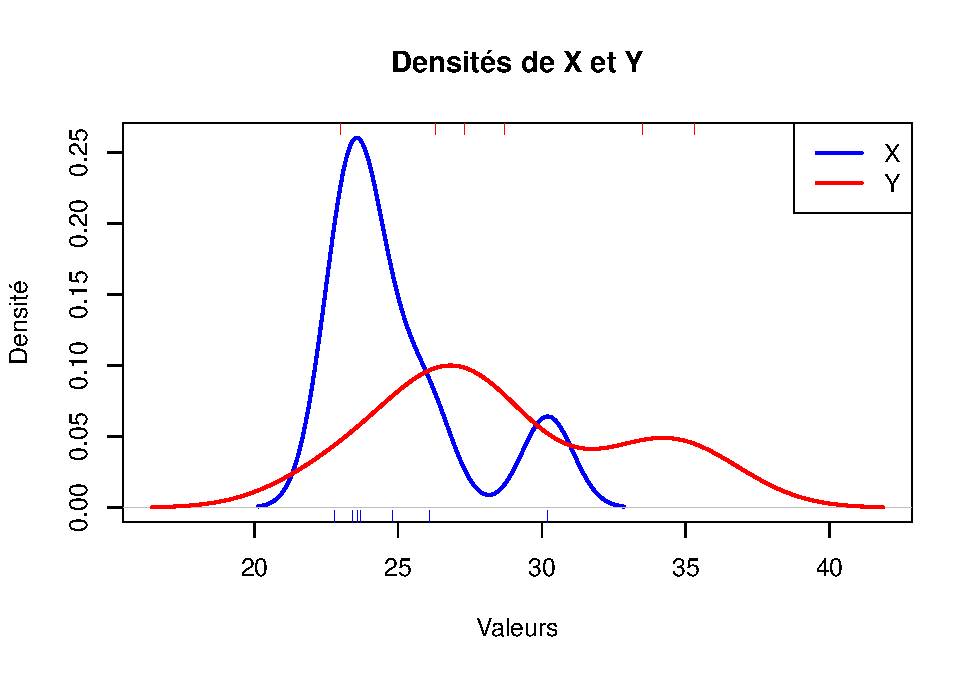
\includegraphics{Stat_non_para_files/figure-latex/unnamed-chunk-84-1.pdf}

\begin{Shaded}
\begin{Highlighting}[]
 \CommentTok{\# —Calcul le rang des éléments de l’échantillon global}
 
\NormalTok{ vecteur\_rang}\OtherTok{\textless{}{-}}\FunctionTok{rank}\NormalTok{(X\_Y, }\AttributeTok{ties.method =} \StringTok{"average"}\NormalTok{)}
\NormalTok{ vecteur\_rang}
\end{Highlighting}
\end{Shaded}

\begin{verbatim}
##  [1]  1.0  3.0  4.0  5.0  6.0  7.0 12.0  2.0  8.5  8.5 10.0 11.0 13.0 14.0
\end{verbatim}

\begin{Shaded}
\begin{Highlighting}[]
 \CommentTok{\# —Calcul de la statistique observée}
 
\NormalTok{ W\_obs }\OtherTok{=} \SpecialCharTok{{-}}\FloatTok{0.5}\SpecialCharTok{*}\FunctionTok{length}\NormalTok{(X)}\SpecialCharTok{*}\NormalTok{(}\FunctionTok{length}\NormalTok{(X)}\SpecialCharTok{+}\DecValTok{1}\NormalTok{)}
 \ControlFlowTok{for}\NormalTok{(i }\ControlFlowTok{in} \DecValTok{1}\SpecialCharTok{:} \FunctionTok{length}\NormalTok{(X))\{}
\NormalTok{ W\_obs}\OtherTok{=}\NormalTok{W\_obs}\SpecialCharTok{+}\NormalTok{vecteur\_rang[i]}
\NormalTok{ \}}
\NormalTok{ W\_obs}
\end{Highlighting}
\end{Shaded}

\begin{verbatim}
## [1] 10
\end{verbatim}

\begin{Shaded}
\begin{Highlighting}[]
 \CommentTok{\# —Décision :}
 
\NormalTok{ alpha }\OtherTok{=} \FloatTok{0.05}
\NormalTok{quantile\_droite }\OtherTok{\textless{}{-}} \FunctionTok{qwilcox}\NormalTok{(}\DecValTok{1} \SpecialCharTok{{-}}\NormalTok{ alpha,n,m,}\AttributeTok{log.p=} \ConstantTok{FALSE}\NormalTok{)}

\ControlFlowTok{if}\NormalTok{(W\_obs }\SpecialCharTok{\textgreater{}=}\NormalTok{ quantile\_droite)\{}
\StringTok{"On rejette l\textquotesingle{}hypothese nulle  "}
\NormalTok{\}}\ControlFlowTok{else}\NormalTok{\{}
\StringTok{"On ne rejette pas l\textquotesingle{}hypothèse nulle"}
\NormalTok{\}}
\end{Highlighting}
\end{Shaded}

\begin{verbatim}
## [1] "On ne rejette pas l'hypothèse nulle"
\end{verbatim}

\textbf{Test unilatéral à gauche}

\begin{Shaded}
\begin{Highlighting}[]
\NormalTok{alpha }\OtherTok{=} \FloatTok{0.05}
\NormalTok{quantile\_gauche }\OtherTok{\textless{}{-}} \FunctionTok{qwilcox}\NormalTok{(alpha,n,m,}\AttributeTok{lower.tail =}\ConstantTok{TRUE}\NormalTok{, }\AttributeTok{log.p=} \ConstantTok{FALSE}\NormalTok{) }
\CommentTok{\# P(W≤q)≤0.05m c\textquotesingle{}est d\textquotesingle{}ailleurs par defaut.}
 
\ControlFlowTok{if}\NormalTok{(W\_obs }\SpecialCharTok{\textless{}=}\NormalTok{ quantile\_gauche)\{}
\StringTok{"On rejette l\textquotesingle{}hypothese nulle  "}
\NormalTok{\}}\ControlFlowTok{else}\NormalTok{\{}
\StringTok{"On ne rejette pas l\textquotesingle{}hypothèse nulle"}
\NormalTok{\}}
\end{Highlighting}
\end{Shaded}

\begin{verbatim}
## [1] "On rejette l'hypothese nulle  "
\end{verbatim}

\textbf{Test bilatéral}

\begin{Shaded}
\begin{Highlighting}[]
\NormalTok{alpha }\OtherTok{=} \FloatTok{0.05}
\NormalTok{q\_low }\OtherTok{\textless{}{-}} \FunctionTok{qwilcox}\NormalTok{(alpha }\SpecialCharTok{/} \DecValTok{2}\NormalTok{, n,m)}
\NormalTok{q\_high }\OtherTok{\textless{}{-}} \FunctionTok{qwilcox}\NormalTok{(}\DecValTok{1} \SpecialCharTok{{-}}\NormalTok{ alpha }\SpecialCharTok{/} \DecValTok{2}\NormalTok{, n,m)}

\ControlFlowTok{if}\NormalTok{(W\_obs }\SpecialCharTok{\textless{}=}\NormalTok{ q\_low }\SpecialCharTok{||}\NormalTok{ W\_obs }\SpecialCharTok{\textgreater{}=}\NormalTok{ q\_high)\{}
\StringTok{"On rejette l\textquotesingle{}hypothese nulle  "}
\NormalTok{\}}\ControlFlowTok{else}\NormalTok{\{}
\StringTok{"On ne rejette pas l\textquotesingle{}hypothèse nulle"}
\NormalTok{\}}
\end{Highlighting}
\end{Shaded}

\begin{verbatim}
## [1] "On ne rejette pas l'hypothèse nulle"
\end{verbatim}

\textbf{Fonction recapitulative}

\begin{Shaded}
\begin{Highlighting}[]
\NormalTok{wilcox\_decision }\OtherTok{\textless{}{-}} \ControlFlowTok{function}\NormalTok{(W\_obs, n, m, }\AttributeTok{alpha =} \FloatTok{0.05}\NormalTok{, }
                            \AttributeTok{alternative =} \FunctionTok{c}\NormalTok{(}\StringTok{"two.sided"}\NormalTok{, }\StringTok{"less"}\NormalTok{, }\StringTok{"greater"}\NormalTok{)) \{}
\NormalTok{  alternative }\OtherTok{\textless{}{-}} \FunctionTok{match.arg}\NormalTok{(alternative)}
  
\ControlFlowTok{if}\NormalTok{ (alternative }\SpecialCharTok{==} \StringTok{"less"}\NormalTok{) \{}
  \CommentTok{\# Test unilatéral à gauche}
\NormalTok{  q\_left }\OtherTok{\textless{}{-}} \FunctionTok{qwilcox}\NormalTok{(alpha,  n, m)}
  
  \ControlFlowTok{if}\NormalTok{ (W\_obs }\SpecialCharTok{\textless{}=}\NormalTok{ q\_left) \{}
    \FunctionTok{return}\NormalTok{(}\StringTok{" Rejet de H0 : le groupe 1 tend à avoir des valeurs plus PETITES que le groupe 2"}\NormalTok{)}
\NormalTok{  \} }\ControlFlowTok{else}\NormalTok{ \{}
    \FunctionTok{return}\NormalTok{(}\StringTok{"✅ On ne rejette pas H0"}\NormalTok{)}
\NormalTok{  \}}
\NormalTok{\}}

   \CommentTok{\# Test unilatéral à droite}
  \ControlFlowTok{else} \ControlFlowTok{if}\NormalTok{ (alternative }\SpecialCharTok{==} \StringTok{"greater"}\NormalTok{) \{}
\NormalTok{    q\_right }\OtherTok{\textless{}{-}} \FunctionTok{qwilcox}\NormalTok{(}\DecValTok{1} \SpecialCharTok{{-}}\NormalTok{ alpha,  n, m)}
    \ControlFlowTok{if}\NormalTok{ (W\_obs }\SpecialCharTok{\textgreater{}=}\NormalTok{ q\_right) \{}
      \FunctionTok{return}\NormalTok{(}\StringTok{"🟥 Rejet de H0 : le groupe 1 tend à avoir des valeurs plus GRANDES que le groupe 2"}\NormalTok{)}
\NormalTok{    \} }\ControlFlowTok{else}\NormalTok{ \{}
      \FunctionTok{return}\NormalTok{(}\StringTok{"✅ On ne rejette pas H0"}\NormalTok{)}
\NormalTok{    \}}
\NormalTok{    \} }
  
  \CommentTok{\# Test bilatéral}
  \ControlFlowTok{else}\NormalTok{ \{}
\NormalTok{    q\_low }\OtherTok{\textless{}{-}} \FunctionTok{qwilcox}\NormalTok{(alpha }\SpecialCharTok{/} \DecValTok{2}\NormalTok{,  n, m)}
\NormalTok{    q\_high }\OtherTok{\textless{}{-}} \FunctionTok{qwilcox}\NormalTok{(}\DecValTok{1} \SpecialCharTok{{-}}\NormalTok{ alpha }\SpecialCharTok{/} \DecValTok{2}\NormalTok{,  n, m)}
    
    \ControlFlowTok{if}\NormalTok{ (W\_obs }\SpecialCharTok{\textless{}=}\NormalTok{ q\_low }\SpecialCharTok{||}\NormalTok{ W\_obs }\SpecialCharTok{\textgreater{}=}\NormalTok{ q\_high) \{}
      \FunctionTok{return}\NormalTok{(}\StringTok{"🟥 Rejet de H0 : les distributions des deux groupes sont significativement différentes"}\NormalTok{)}
\NormalTok{    \} }\ControlFlowTok{else}\NormalTok{ \{}
      \FunctionTok{return}\NormalTok{(}\StringTok{"✅ On ne rejette pas H0"}\NormalTok{)}
\NormalTok{    \}}
\NormalTok{  \}}
\NormalTok{\}}
\end{Highlighting}
\end{Shaded}

\textbf{Application}

\begin{Shaded}
\begin{Highlighting}[]
\FunctionTok{wilcox\_decision}\NormalTok{(W\_obs,  n, m, }\AttributeTok{alpha =} \FloatTok{0.05}\NormalTok{, }\AttributeTok{alternative =} \StringTok{"two.sided"}\NormalTok{)}
\end{Highlighting}
\end{Shaded}

\begin{verbatim}
## [1] "✅ On ne rejette pas H0"
\end{verbatim}

\begin{Shaded}
\begin{Highlighting}[]
\FunctionTok{wilcox\_decision}\NormalTok{(W\_obs,  n, m, }\AttributeTok{alternative =} \StringTok{"less"}\NormalTok{)}
\end{Highlighting}
\end{Shaded}

\begin{verbatim}
## [1] " Rejet de H0 : le groupe 1 tend à avoir des valeurs plus PETITES que le groupe 2"
\end{verbatim}

\begin{Shaded}
\begin{Highlighting}[]
\FunctionTok{wilcox\_decision}\NormalTok{(W\_obs,  n, m, }\AttributeTok{alternative =} \StringTok{"greater"}\NormalTok{)}
\end{Highlighting}
\end{Shaded}

\begin{verbatim}
## [1] "✅ On ne rejette pas H0"
\end{verbatim}

\textbf{Test avec la loi normale}

\begin{Shaded}
\begin{Highlighting}[]
\DocumentationTok{\#\# Approximation avec la loi normale}
\NormalTok{E }\OtherTok{\textless{}{-}}\NormalTok{ n}\SpecialCharTok{*}\NormalTok{(n}\SpecialCharTok{+}\NormalTok{m}\SpecialCharTok{+}\DecValTok{1}\NormalTok{)}\SpecialCharTok{/}\DecValTok{2} \SpecialCharTok{{-}}\NormalTok{ n}\SpecialCharTok{*}\NormalTok{(n}\SpecialCharTok{+}\DecValTok{1}\NormalTok{)}\SpecialCharTok{/}\DecValTok{2}  \CommentTok{\# Correction de la formule d\textquotesingle{}espérance}
\NormalTok{Var }\OtherTok{\textless{}{-}}\NormalTok{ (n}\SpecialCharTok{*}\NormalTok{m}\SpecialCharTok{*}\NormalTok{(n}\SpecialCharTok{+}\NormalTok{m}\SpecialCharTok{+}\DecValTok{1}\NormalTok{))}\SpecialCharTok{/}\DecValTok{12}        \CommentTok{\# Correction de la formule de variance}

\NormalTok{Z }\OtherTok{\textless{}{-}}\NormalTok{ (W\_obs }\SpecialCharTok{{-}}\NormalTok{ E)}\SpecialCharTok{/}\FunctionTok{sqrt}\NormalTok{(Var)     }\CommentTok{\# Statistique standardisée}

\CommentTok{\# Calcul des p{-}values selon le type de test}
\NormalTok{p\_value\_bilateral }\OtherTok{\textless{}{-}} \DecValTok{2}\SpecialCharTok{*}\FunctionTok{pnorm}\NormalTok{(}\SpecialCharTok{{-}}\FunctionTok{abs}\NormalTok{(Z))}
\NormalTok{p\_value\_gauche }\OtherTok{\textless{}{-}} \FunctionTok{pnorm}\NormalTok{(Z)}
\NormalTok{p\_value\_droite }\OtherTok{\textless{}{-}} \DecValTok{1} \SpecialCharTok{{-}} \FunctionTok{pnorm}\NormalTok{(Z)}

\CommentTok{\# Fonction de décision normalisée}
\NormalTok{wilcox\_normal\_decision }\OtherTok{\textless{}{-}} \ControlFlowTok{function}\NormalTok{(Z, }\AttributeTok{alpha =} \FloatTok{0.05}\NormalTok{, }\AttributeTok{alternative =} \FunctionTok{c}\NormalTok{(}\StringTok{"two.sided"}\NormalTok{, }\StringTok{"less"}\NormalTok{, }\StringTok{"greater"}\NormalTok{)) \{}
\NormalTok{  alternative }\OtherTok{\textless{}{-}} \FunctionTok{match.arg}\NormalTok{(alternative)}
  
  \ControlFlowTok{if}\NormalTok{ (alternative }\SpecialCharTok{==} \StringTok{"less"}\NormalTok{) \{}
\NormalTok{    p\_value }\OtherTok{\textless{}{-}} \FunctionTok{pnorm}\NormalTok{(Z)}
    \ControlFlowTok{if}\NormalTok{ (p\_value }\SpecialCharTok{\textless{}}\NormalTok{ alpha) \{}
      \FunctionTok{return}\NormalTok{(}\FunctionTok{list}\NormalTok{(}
        \AttributeTok{decision =} \StringTok{"🟥 Rejet de H0 (approximation normale) : X tend à avoir des valeurs plus petites que Y"}\NormalTok{,}
        \AttributeTok{p\_value =}\NormalTok{ p\_value,}
        \AttributeTok{Z =}\NormalTok{ Z}
\NormalTok{      ))}
\NormalTok{    \} }\ControlFlowTok{else}\NormalTok{ \{}
      \FunctionTok{return}\NormalTok{(}\FunctionTok{list}\NormalTok{(}
        \AttributeTok{decision =} \StringTok{"✅ On ne rejette pas H0 (approximation normale)"}\NormalTok{,}
        \AttributeTok{p\_value =}\NormalTok{ p\_value,}
        \AttributeTok{Z =}\NormalTok{ Z}
\NormalTok{      ))}
\NormalTok{    \}}
\NormalTok{  \}}
  \ControlFlowTok{else} \ControlFlowTok{if}\NormalTok{ (alternative }\SpecialCharTok{==} \StringTok{"greater"}\NormalTok{) \{}
\NormalTok{    p\_value }\OtherTok{\textless{}{-}} \DecValTok{1} \SpecialCharTok{{-}} \FunctionTok{pnorm}\NormalTok{(Z)}
    \ControlFlowTok{if}\NormalTok{ (p\_value }\SpecialCharTok{\textless{}}\NormalTok{ alpha) \{}
      \FunctionTok{return}\NormalTok{(}\FunctionTok{list}\NormalTok{(}
        \AttributeTok{decision =} \StringTok{"🟥 Rejet de H0 (approximation normale) : X tend à avoir des valeurs plus grandes que Y"}\NormalTok{,}
        \AttributeTok{p\_value =}\NormalTok{ p\_value,}
        \AttributeTok{Z =}\NormalTok{ Z}
\NormalTok{      ))}
\NormalTok{    \} }\ControlFlowTok{else}\NormalTok{ \{}
      \FunctionTok{return}\NormalTok{(}\FunctionTok{list}\NormalTok{(}
        \AttributeTok{decision =} \StringTok{"✅ On ne rejette pas H0 (approximation normale)"}\NormalTok{,}
        \AttributeTok{p\_value =}\NormalTok{ p\_value,}
        \AttributeTok{Z =}\NormalTok{ Z}
\NormalTok{      ))}
\NormalTok{    \}}
\NormalTok{  \}}
  \ControlFlowTok{else}\NormalTok{ \{}
\NormalTok{    p\_value }\OtherTok{\textless{}{-}} \DecValTok{2}\SpecialCharTok{*}\FunctionTok{pnorm}\NormalTok{(}\SpecialCharTok{{-}}\FunctionTok{abs}\NormalTok{(Z))}
    \ControlFlowTok{if}\NormalTok{ (p\_value }\SpecialCharTok{\textless{}}\NormalTok{ alpha) \{}
      \FunctionTok{return}\NormalTok{(}\FunctionTok{list}\NormalTok{(}
        \AttributeTok{decision =} \StringTok{"🟥 Rejet de H0 (approximation normale) : Distributions significativement différentes"}\NormalTok{,}
        \AttributeTok{p\_value =}\NormalTok{ p\_value,}
        \AttributeTok{Z =}\NormalTok{ Z}
\NormalTok{      ))}
\NormalTok{    \} }\ControlFlowTok{else}\NormalTok{ \{}
      \FunctionTok{return}\NormalTok{(}\FunctionTok{list}\NormalTok{(}
        \AttributeTok{decision =} \StringTok{"✅ On ne rejette pas H0 (approximation normale)"}\NormalTok{,}
        \AttributeTok{p\_value =}\NormalTok{ p\_value,}
        \AttributeTok{Z =}\NormalTok{ Z}
\NormalTok{      ))}
\NormalTok{    \}}
\NormalTok{  \}}
\NormalTok{\}}

\DocumentationTok{\#\# Application}
\NormalTok{result\_bilateral }\OtherTok{\textless{}{-}} \FunctionTok{wilcox\_normal\_decision}\NormalTok{(Z, }\AttributeTok{alternative =} \StringTok{"two.sided"}\NormalTok{)}
\NormalTok{result\_gauche }\OtherTok{\textless{}{-}} \FunctionTok{wilcox\_normal\_decision}\NormalTok{(Z, }\AttributeTok{alternative =} \StringTok{"less"}\NormalTok{)}
\NormalTok{result\_droite }\OtherTok{\textless{}{-}} \FunctionTok{wilcox\_normal\_decision}\NormalTok{(Z, }\AttributeTok{alternative =} \StringTok{"greater"}\NormalTok{)}

\CommentTok{\# Affichage des résultats}
\FunctionTok{cat}\NormalTok{(}\StringTok{"Test bilatéral:}\SpecialCharTok{\textbackslash{}n}\StringTok{"}\NormalTok{)}
\end{Highlighting}
\end{Shaded}

\begin{verbatim}
## Test bilatéral:
\end{verbatim}

\begin{Shaded}
\begin{Highlighting}[]
\FunctionTok{cat}\NormalTok{(}\StringTok{"Z ="}\NormalTok{, }\FunctionTok{round}\NormalTok{(result\_bilateral}\SpecialCharTok{$}\NormalTok{Z, }\DecValTok{3}\NormalTok{), }\StringTok{"| p{-}value ="}\NormalTok{, result\_bilateral}\SpecialCharTok{$}\NormalTok{p\_value, }\StringTok{"}\SpecialCharTok{\textbackslash{}n}\StringTok{"}\NormalTok{)}
\end{Highlighting}
\end{Shaded}

\begin{verbatim}
## Z = -1.853 | p-value = 0.06391934
\end{verbatim}

\begin{Shaded}
\begin{Highlighting}[]
\FunctionTok{cat}\NormalTok{(result\_bilateral}\SpecialCharTok{$}\NormalTok{decision, }\StringTok{"}\SpecialCharTok{\textbackslash{}n\textbackslash{}n}\StringTok{"}\NormalTok{)}
\end{Highlighting}
\end{Shaded}

\begin{verbatim}
## ✅ On ne rejette pas H0 (approximation normale)
\end{verbatim}

\begin{Shaded}
\begin{Highlighting}[]
\FunctionTok{cat}\NormalTok{(}\StringTok{"Test unilatéral à gauche:}\SpecialCharTok{\textbackslash{}n}\StringTok{"}\NormalTok{)}
\end{Highlighting}
\end{Shaded}

\begin{verbatim}
## Test unilatéral à gauche:
\end{verbatim}

\begin{Shaded}
\begin{Highlighting}[]
\FunctionTok{cat}\NormalTok{(}\StringTok{"Z ="}\NormalTok{, }\FunctionTok{round}\NormalTok{(result\_gauche}\SpecialCharTok{$}\NormalTok{Z, }\DecValTok{3}\NormalTok{), }\StringTok{"| p{-}value ="}\NormalTok{, result\_gauche}\SpecialCharTok{$}\NormalTok{p\_value, }\StringTok{"}\SpecialCharTok{\textbackslash{}n}\StringTok{"}\NormalTok{)}
\end{Highlighting}
\end{Shaded}

\begin{verbatim}
## Z = -1.853 | p-value = 0.03195967
\end{verbatim}

\begin{Shaded}
\begin{Highlighting}[]
\FunctionTok{cat}\NormalTok{(result\_gauche}\SpecialCharTok{$}\NormalTok{decision, }\StringTok{"}\SpecialCharTok{\textbackslash{}n\textbackslash{}n}\StringTok{"}\NormalTok{)}
\end{Highlighting}
\end{Shaded}

\begin{verbatim}
## 🟥 Rejet de H0 (approximation normale) : X tend à avoir des valeurs plus petites que Y
\end{verbatim}

\begin{Shaded}
\begin{Highlighting}[]
\FunctionTok{cat}\NormalTok{(}\StringTok{"Test unilatéral à droite:}\SpecialCharTok{\textbackslash{}n}\StringTok{"}\NormalTok{)}
\end{Highlighting}
\end{Shaded}

\begin{verbatim}
## Test unilatéral à droite:
\end{verbatim}

\begin{Shaded}
\begin{Highlighting}[]
\FunctionTok{cat}\NormalTok{(}\StringTok{"Z ="}\NormalTok{, }\FunctionTok{round}\NormalTok{(result\_droite}\SpecialCharTok{$}\NormalTok{Z, }\DecValTok{3}\NormalTok{), }\StringTok{"| p{-}value ="}\NormalTok{, result\_droite}\SpecialCharTok{$}\NormalTok{p\_value, }\StringTok{"}\SpecialCharTok{\textbackslash{}n}\StringTok{"}\NormalTok{)}
\end{Highlighting}
\end{Shaded}

\begin{verbatim}
## Z = -1.853 | p-value = 0.9680403
\end{verbatim}

\begin{Shaded}
\begin{Highlighting}[]
\FunctionTok{cat}\NormalTok{(result\_droite}\SpecialCharTok{$}\NormalTok{decision, }\StringTok{"}\SpecialCharTok{\textbackslash{}n}\StringTok{"}\NormalTok{)}
\end{Highlighting}
\end{Shaded}

\begin{verbatim}
## ✅ On ne rejette pas H0 (approximation normale)
\end{verbatim}

\textbf{Avec la fonction disponible dans R}

\begin{Shaded}
\begin{Highlighting}[]
\FunctionTok{wilcox.test}\NormalTok{(X,Y,}\AttributeTok{alternative=}\StringTok{"two.side"}\NormalTok{)}
\end{Highlighting}
\end{Shaded}

\begin{verbatim}
## 
##  Wilcoxon rank sum test with continuity correction
## 
## data:  X and Y
## W = 10, p-value = 0.07332
## alternative hypothesis: true location shift is not equal to 0
\end{verbatim}

\subsection{Tests d'alternative
d'échelle}\label{tests-dalternative-duxe9chelle}

\subsubsection{Test de Savage}\label{test-de-savage}

\textbf{Présentation du Test de Savage :}

Soient \(X\) une variable continue et \(Y\) une variable catégorielle de
modalités : \(y_1, y_2, \dots , y_K\). Le test de savage permet de
tester si les sous échantillons de \(X\) en fonction de \(Y\) :
\(X|_{Y=y_1},  \ldots,  X|_{Y=y_K }\) ont la même fonction de
répartition.

Pour le test, on construit une fonction de score répartissant la
distribution des rangs de X autour de leur position centrale moyenne.\\
la formule de la fonction de score est la suivante :

\[f(r_i) = \sum_{j=r_i}^{n} \frac{1}{j}  = \sum_{j=1}^{n-r_i+1} \frac{1}{j} - 1 \]

où \(r_i\) est le rang de l'observation \(i\) et \(n\) la taille totale
de l'échantillon.

\textbf{Statistique de Test :}

La statistique de test a alors pour formule :

\[S = \frac{\sum_{k=1}^{K} \frac{(T_k - n_k \bar{f})^2}{n_k}}{\frac{\sum_{i=1}^{n} (f_i - \bar{f})^2}{n-1}}\]

Avec :

\begin{itemize}
\tightlist
\item
  \(T_k\) = somme des scores de Savage pour le groupe \(k\)
\item
  \(n_k\) = effectif du groupe \(k\)
\item
  \(\bar{f}\) = moyenne des scores de Savage
\item
  \(K\) = nombre de groupes
\end{itemize}

\paragraph{Hypothèses du Test}\label{hypothuxe8ses-du-test}

La statistique suit une loi du \(\chi^2\) à \((K-1)\) degrés de liberté
et l'hypothèse \(H_0\) est :

\[H_0 : F_1(x) = F_2(x) = \ldots = F_K(x)\]

Avec la valeur seuil \(\chi^2_{1-\alpha, K-1}\) de la distribution de la
statistique de test du \(\chi^2\) pour une confiance \((1-\alpha)\) et
pour \((K-1)\) degrés de liberté, l'hypothèse alternative est alors :

\(H_1 : \exists i,j \in \{1,2,\ldots,K\} : F_i(x) \neq F_j(x)\)

\begin{itemize}
\tightlist
\item
  tel que \(S > \chi^2_{1-\alpha, k-1}\), soit rejet de \(H_0\), pour un
  test bilatéral
\item
  Le test du \(\chi^2\) ne propose pas de forme unilatérale à droite ou
  à gauche pour \(S\)
\end{itemize}

La loi à laquelle reporter la statistique de test de Savage est celle du
\(\chi^2\) à \((k-1)\) degrés de liberté. La formule de la p-valeur
exacte est alors :

\[p = P(\chi^2_{K-1} > S) = 1 - F_{\chi^2_{K-1}}(S)\]

\textbf{Tendance pour le rejet de l'hypothèse nulle}

Plus la statistique de test de Savage est grande et plus on a de chance
de rejeter \(H_0\), ce qui revient à dire que :

\begin{itemize}
\item
  \textbf{On rejette} \(H_0\) si \(S > \chi^2_{1-\alpha, K-1}\)
\item
  Soit que la somme des rangs pour l'un des groupes est nettement plus
  grande que la moyenne des rangs pondérés, impliquant que l'une des
  distributions est nettement différente des autres.
\item
  \textbf{Tendance lorsque n tend vers l'infini}
\end{itemize}

Le test de Savage est influencé par la taille de l'échantillon. Pour de
très grands échantillons, le test peut rejeter \(H_0\) à tort même
lorsque les distributions sont similaires. Cette sensibilité est due à
la formule de la statistique de test qui fait intervenir les effectifs
des différents groupes.

\paragraph{Implémentation}\label{impluxe9mentation}

\begin{itemize}
\tightlist
\item
  \textbf{Importation des données}
\end{itemize}

\begin{Shaded}
\begin{Highlighting}[]
\NormalTok{donnees }\OtherTok{\textless{}{-}} \FunctionTok{read\_dta}\NormalTok{(}\StringTok{"BASES/savage\_dataset.dta"}\NormalTok{)}
\NormalTok{donnees}\SpecialCharTok{$}\NormalTok{milieu }\OtherTok{\textless{}{-}} \FunctionTok{as\_factor}\NormalTok{(donnees}\SpecialCharTok{$}\NormalTok{milieu)}
\end{Highlighting}
\end{Shaded}

\begin{itemize}
\tightlist
\item
  \textbf{Graphique des courbes de densité par classe}
\end{itemize}

\begin{Shaded}
\begin{Highlighting}[]
\NormalTok{plot\_densites }\OtherTok{\textless{}{-}} \ControlFlowTok{function}\NormalTok{(data, var\_continue, var\_groupe, }
                          \AttributeTok{titre =} \StringTok{"Distribution par groupe"}\NormalTok{) \{}
  
  \CommentTok{\# Création du graphique de densité}
\NormalTok{  p }\OtherTok{\textless{}{-}} \FunctionTok{ggplot}\NormalTok{(data, }\FunctionTok{aes\_string}\NormalTok{(}\AttributeTok{x =}\NormalTok{ var\_continue, }\AttributeTok{color =}\NormalTok{ var\_groupe)) }\SpecialCharTok{+}
    \FunctionTok{geom\_density}\NormalTok{(}\AttributeTok{size =} \FloatTok{1.2}\NormalTok{, }\AttributeTok{alpha =} \FloatTok{0.8}\NormalTok{) }\SpecialCharTok{+}
    \FunctionTok{theme\_minimal}\NormalTok{() }\SpecialCharTok{+}
    \FunctionTok{labs}\NormalTok{(}
      \AttributeTok{title =}\NormalTok{ titre,}
      \AttributeTok{x =}\NormalTok{ var\_continue,}
      \AttributeTok{y =} \StringTok{"Densité"}\NormalTok{,}
      \AttributeTok{color =}\NormalTok{ var\_groupe}
\NormalTok{    ) }\SpecialCharTok{+}
    \FunctionTok{theme}\NormalTok{(}
      \AttributeTok{legend.position =} \StringTok{"bottom"}\NormalTok{,}
      \AttributeTok{plot.title =} \FunctionTok{element\_text}\NormalTok{(}\AttributeTok{hjust =} \FloatTok{0.5}\NormalTok{, }\AttributeTok{size =} \DecValTok{14}\NormalTok{, }\AttributeTok{face =} \StringTok{"bold"}\NormalTok{),}
      \AttributeTok{axis.title =} \FunctionTok{element\_text}\NormalTok{(}\AttributeTok{size =} \DecValTok{12}\NormalTok{),}
      \AttributeTok{legend.title =} \FunctionTok{element\_text}\NormalTok{(}\AttributeTok{size =} \DecValTok{12}\NormalTok{)}
\NormalTok{    )}
  
  \FunctionTok{return}\NormalTok{(p)}
\NormalTok{\}}
\end{Highlighting}
\end{Shaded}

\begin{itemize}
\tightlist
\item
  \textbf{Boxplot par classe}
\end{itemize}

\begin{Shaded}
\begin{Highlighting}[]
\NormalTok{plot\_boxplots }\OtherTok{\textless{}{-}} \ControlFlowTok{function}\NormalTok{(data, var\_continue, var\_groupe, }
                          \AttributeTok{titre =} \StringTok{"Boxplot par groupe"}\NormalTok{) \{}
  
  \CommentTok{\# Création du boxplot}
\NormalTok{  p }\OtherTok{\textless{}{-}} \FunctionTok{ggplot}\NormalTok{(data, }\FunctionTok{aes\_string}\NormalTok{(}\AttributeTok{x =}\NormalTok{ var\_groupe, }\AttributeTok{y =}\NormalTok{ var\_continue, }\AttributeTok{fill =}\NormalTok{ var\_groupe)) }\SpecialCharTok{+}
    \FunctionTok{geom\_boxplot}\NormalTok{(}\AttributeTok{alpha =} \FloatTok{0.7}\NormalTok{, }\AttributeTok{outlier.color =} \StringTok{"red"}\NormalTok{, }\AttributeTok{outlier.size =} \DecValTok{2}\NormalTok{) }\SpecialCharTok{+}
    \FunctionTok{theme\_minimal}\NormalTok{() }\SpecialCharTok{+}
    \FunctionTok{labs}\NormalTok{(}
      \AttributeTok{title =}\NormalTok{ titre,}
      \AttributeTok{x =}\NormalTok{ var\_groupe,}
      \AttributeTok{y =}\NormalTok{ var\_continue,}
      \AttributeTok{fill =}\NormalTok{ var\_groupe}
\NormalTok{    ) }\SpecialCharTok{+}
    \FunctionTok{theme}\NormalTok{(}
      \AttributeTok{legend.position =} \StringTok{"none"}\NormalTok{,}
      \AttributeTok{plot.title =} \FunctionTok{element\_text}\NormalTok{(}\AttributeTok{hjust =} \FloatTok{0.5}\NormalTok{, }\AttributeTok{size =} \DecValTok{14}\NormalTok{, }\AttributeTok{face =} \StringTok{"bold"}\NormalTok{),}
      \AttributeTok{axis.title =} \FunctionTok{element\_text}\NormalTok{(}\AttributeTok{size =} \DecValTok{12}\NormalTok{),}
      \AttributeTok{axis.text.x =} \FunctionTok{element\_text}\NormalTok{(}\AttributeTok{angle =} \DecValTok{45}\NormalTok{, }\AttributeTok{hjust =} \DecValTok{1}\NormalTok{)}
\NormalTok{    )}
  
  \FunctionTok{return}\NormalTok{(p)}
\NormalTok{\}}
\end{Highlighting}
\end{Shaded}

\begin{itemize}
\tightlist
\item
  \textbf{Affichage des courbes de densité}
\end{itemize}

\begin{Shaded}
\begin{Highlighting}[]
\FunctionTok{plot\_densites}\NormalTok{(donnees, }\StringTok{"age"}\NormalTok{, }\StringTok{"milieu"}\NormalTok{, }\StringTok{"Distribution des âges par milieu de résidence"}\NormalTok{)}
\end{Highlighting}
\end{Shaded}

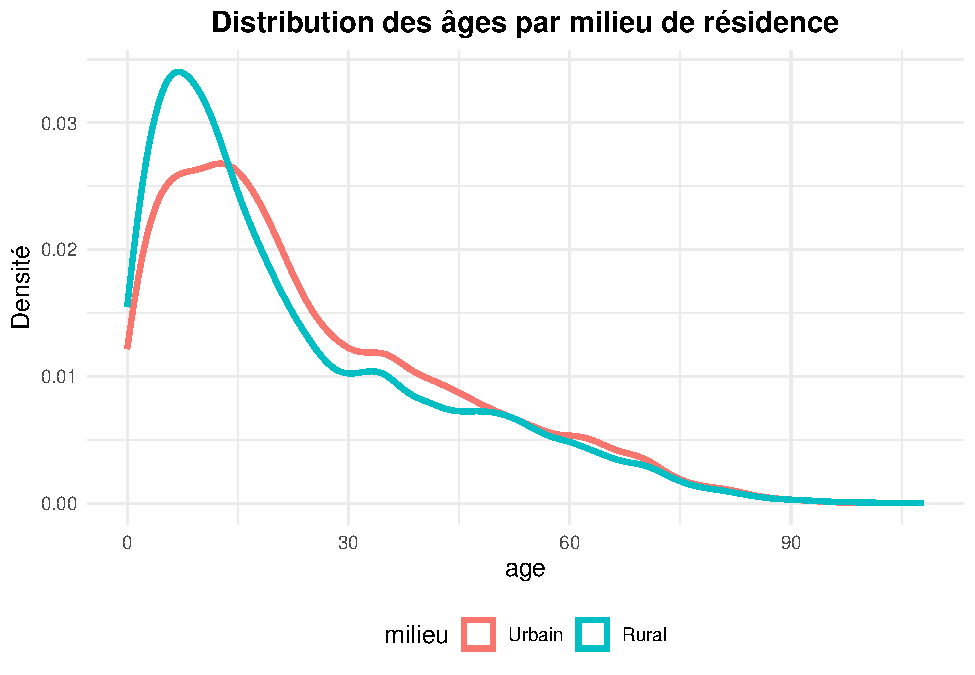
\includegraphics{Stat_non_para_files/figure-latex/unnamed-chunk-95-1.pdf}

\begin{itemize}
\tightlist
\item
  \textbf{Affichage des boxplots}
\end{itemize}

\begin{Shaded}
\begin{Highlighting}[]
\FunctionTok{plot\_boxplots}\NormalTok{(donnees, }\StringTok{"age"}\NormalTok{, }\StringTok{"milieu"}\NormalTok{, }\StringTok{"Boxplot des âges par milieu de résidence"}\NormalTok{)}
\end{Highlighting}
\end{Shaded}

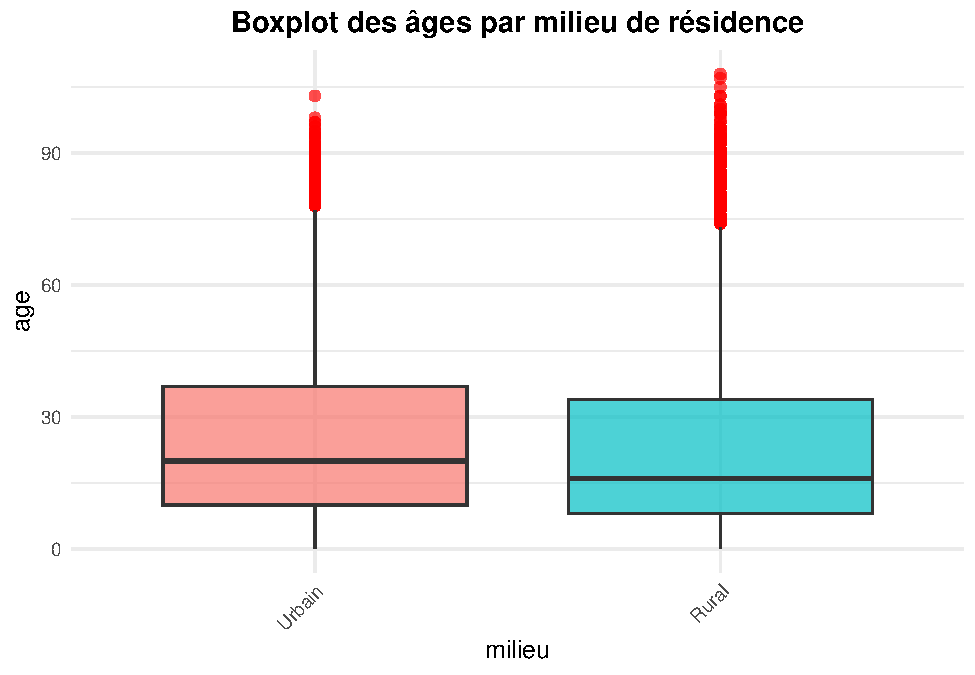
\includegraphics{Stat_non_para_files/figure-latex/unnamed-chunk-96-1.pdf}

\begin{itemize}
\tightlist
\item
  \textbf{Fonction de test de Savage}
\end{itemize}

\begin{Shaded}
\begin{Highlighting}[]
\NormalTok{SavageTest }\OtherTok{\textless{}{-}} \ControlFlowTok{function}\NormalTok{(X, Y) \{}
  
  \CommentTok{\# Vérifications préliminaires}
  \ControlFlowTok{if}\NormalTok{(}\FunctionTok{length}\NormalTok{(X) }\SpecialCharTok{!=} \FunctionTok{length}\NormalTok{(Y)) \{}
    \FunctionTok{stop}\NormalTok{(}\StringTok{"Les vecteurs X et Y doivent avoir la même longueur"}\NormalTok{)}
\NormalTok{  \}}
  
  \ControlFlowTok{if}\NormalTok{(}\FunctionTok{any}\NormalTok{(}\FunctionTok{is.na}\NormalTok{(X)) }\SpecialCharTok{||} \FunctionTok{any}\NormalTok{(}\FunctionTok{is.na}\NormalTok{(Y))) \{}
    \FunctionTok{stop}\NormalTok{(}\StringTok{"Les données ne doivent pas contenir de valeurs manquantes"}\NormalTok{)}
\NormalTok{  \}}
  
  \CommentTok{\# Transformation de X en variable de rang}
\NormalTok{  R }\OtherTok{\textless{}{-}} \FunctionTok{rank}\NormalTok{(X)}
  
  \CommentTok{\# Récupération des différents éléments}
\NormalTok{  n }\OtherTok{\textless{}{-}} \FunctionTok{length}\NormalTok{(R)}
\NormalTok{  biblio }\OtherTok{\textless{}{-}} \FunctionTok{summary}\NormalTok{(}\FunctionTok{factor}\NormalTok{(Y)) }\CommentTok{\#effectif de chaque groupe}
\NormalTok{  nbClass }\OtherTok{\textless{}{-}} \FunctionTok{length}\NormalTok{(biblio)}
  
  \CommentTok{\# Vérification du nombre de groupes}
  \ControlFlowTok{if}\NormalTok{(nbClass }\SpecialCharTok{\textless{}} \DecValTok{2}\NormalTok{) \{}
    \FunctionTok{stop}\NormalTok{(}\StringTok{"Il faut au moins 2 groupes pour effectuer le test"}\NormalTok{)}
\NormalTok{  \}}
  
  \FunctionTok{print}\NormalTok{(}\FunctionTok{paste}\NormalTok{(}\StringTok{"Nombre d\textquotesingle{}observations:"}\NormalTok{, n))}
  \FunctionTok{print}\NormalTok{(}\FunctionTok{paste}\NormalTok{(}\StringTok{"Nombre de groupes:"}\NormalTok{, nbClass))}
  \FunctionTok{print}\NormalTok{(}\StringTok{"Effectifs par groupe:"}\NormalTok{)}
  \FunctionTok{print}\NormalTok{(biblio)}
  
  \CommentTok{\# Initialisation des vecteurs f}
\NormalTok{  f }\OtherTok{\textless{}{-}} \DecValTok{0} \CommentTok{\# score de savage pour chaque observation}
\NormalTok{  ff }\OtherTok{\textless{}{-}} \DecValTok{0} \CommentTok{\# score de savage par groupe}
  
  \CommentTok{\# Calcul de f(X restreint aux différents groupes de Y)}
  \ControlFlowTok{for}\NormalTok{ (c }\ControlFlowTok{in} \DecValTok{1}\SpecialCharTok{:}\NormalTok{nbClass) \{}
    \CommentTok{\# Focus sur la classe en cours}
\NormalTok{    Rcalc }\OtherTok{\textless{}{-}}\NormalTok{ R[}\FunctionTok{which}\NormalTok{(Y }\SpecialCharTok{==} \FunctionTok{names}\NormalTok{(biblio)[c])]}
\NormalTok{    nb }\OtherTok{\textless{}{-}} \FunctionTok{length}\NormalTok{(Rcalc)}
\NormalTok{    f\_Rcalc }\OtherTok{\textless{}{-}} \DecValTok{0}
\NormalTok{    aa }\OtherTok{\textless{}{-}} \DecValTok{0}
    
    \CommentTok{\# Pour chaque observation de la classe en cours}
    \ControlFlowTok{for}\NormalTok{ (i }\ControlFlowTok{in} \DecValTok{1}\SpecialCharTok{:}\NormalTok{nb) \{}
      \CommentTok{\# Calcul du score de Savage : somme de 1/(n{-}k+1) pour k allant de rang à n}
\NormalTok{      a }\OtherTok{\textless{}{-}} \FunctionTok{sum}\NormalTok{(}\DecValTok{1}\SpecialCharTok{/}\NormalTok{(n }\SpecialCharTok{{-}} \DecValTok{1}\SpecialCharTok{:}\NormalTok{Rcalc[i] }\SpecialCharTok{+} \DecValTok{1}\NormalTok{)) }\SpecialCharTok{{-}} \DecValTok{1}
\NormalTok{      f\_Rcalc }\OtherTok{\textless{}{-}} \FunctionTok{c}\NormalTok{(f\_Rcalc, a)}
\NormalTok{      aa }\OtherTok{\textless{}{-}} \FunctionTok{c}\NormalTok{(aa, a)}
\NormalTok{    \}}
    
    \CommentTok{\# Remplissage des vecteurs}
\NormalTok{    f }\OtherTok{\textless{}{-}} \FunctionTok{c}\NormalTok{(f, f\_Rcalc[}\SpecialCharTok{{-}}\DecValTok{1}\NormalTok{])}
\NormalTok{    ff }\OtherTok{\textless{}{-}} \FunctionTok{c}\NormalTok{(ff, }\FunctionTok{sum}\NormalTok{(aa[}\SpecialCharTok{{-}}\DecValTok{1}\NormalTok{]))}
\NormalTok{  \}}
  
  \CommentTok{\# Calcul du dénominateur et du numérateur}
\NormalTok{  f\_barre }\OtherTok{\textless{}{-}} \FunctionTok{mean}\NormalTok{(f[}\SpecialCharTok{{-}}\DecValTok{1}\NormalTok{])}
\NormalTok{  Denom }\OtherTok{\textless{}{-}} \FunctionTok{sum}\NormalTok{((f[}\SpecialCharTok{{-}}\DecValTok{1}\NormalTok{] }\SpecialCharTok{{-}}\NormalTok{ f\_barre)}\SpecialCharTok{\^{}}\DecValTok{2}\NormalTok{)}\SpecialCharTok{/}\NormalTok{(n }\SpecialCharTok{{-}} \DecValTok{1}\NormalTok{)}
\NormalTok{  Num }\OtherTok{\textless{}{-}} \FunctionTok{sum}\NormalTok{((ff[}\SpecialCharTok{{-}}\DecValTok{1}\NormalTok{] }\SpecialCharTok{{-}}\NormalTok{ biblio}\SpecialCharTok{*}\NormalTok{f\_barre)}\SpecialCharTok{\^{}}\DecValTok{2}\SpecialCharTok{/}\NormalTok{biblio)}
  
  \CommentTok{\# Calcul de la statistique de test}
\NormalTok{  S }\OtherTok{\textless{}{-}}\NormalTok{ Num}\SpecialCharTok{/}\NormalTok{Denom}
\NormalTok{  df }\OtherTok{\textless{}{-}}\NormalTok{ nbClass }\SpecialCharTok{{-}} \DecValTok{1}
\NormalTok{  p\_value }\OtherTok{\textless{}{-}} \DecValTok{1} \SpecialCharTok{{-}} \FunctionTok{pchisq}\NormalTok{(S, df)}
  
  \CommentTok{\# Préparation des résultats}
\NormalTok{  Result }\OtherTok{\textless{}{-}} \FunctionTok{c}\NormalTok{(biblio, }\AttributeTok{N =}\NormalTok{ n, }\AttributeTok{Statistique\_test =}\NormalTok{ S, }\AttributeTok{df =}\NormalTok{ df, }\AttributeTok{p\_value =}\NormalTok{ p\_value)}
  
  \FunctionTok{return}\NormalTok{(Result)}
\NormalTok{\}}
\end{Highlighting}
\end{Shaded}

\begin{itemize}
\tightlist
\item
  \textbf{Fonction d'interprétation complète}
\end{itemize}

\begin{Shaded}
\begin{Highlighting}[]
\NormalTok{interpretation\_savage }\OtherTok{\textless{}{-}} \ControlFlowTok{function}\NormalTok{(X, Y, }\AttributeTok{alpha =} \FloatTok{0.05}\NormalTok{, }\AttributeTok{nom\_var\_X =} \StringTok{"X"}\NormalTok{, }\AttributeTok{nom\_var\_Y =} \StringTok{"Y"}\NormalTok{) \{}
  \CommentTok{\#\textquotesingle{} Fonction complète d\textquotesingle{}interprétation du test de Savage}
  \CommentTok{\#\textquotesingle{} }
  \CommentTok{\#\textquotesingle{} @param X Variable continue}
  \CommentTok{\#\textquotesingle{} @param Y Variable qualitative (groupes)}
  \CommentTok{\#\textquotesingle{} @param alpha Seuil de significativité (défaut: 0.05)}
  \CommentTok{\#\textquotesingle{} @param nom\_var\_X Nom de la variable continue pour l\textquotesingle{}affichage}
  \CommentTok{\#\textquotesingle{} @param nom\_var\_Y Nom de la variable qualitative pour l\textquotesingle{}affichage}
  
  \FunctionTok{cat}\NormalTok{(}\StringTok{"=========================================}\SpecialCharTok{\textbackslash{}n}\StringTok{"}\NormalTok{)}
  \FunctionTok{cat}\NormalTok{(}\StringTok{"           TEST DE SAVAGE}\SpecialCharTok{\textbackslash{}n}\StringTok{"}\NormalTok{)}
  \FunctionTok{cat}\NormalTok{(}\StringTok{"=========================================}\SpecialCharTok{\textbackslash{}n\textbackslash{}n}\StringTok{"}\NormalTok{)}
  
  \FunctionTok{cat}\NormalTok{(}\StringTok{"Variables analysées:}\SpecialCharTok{\textbackslash{}n}\StringTok{"}\NormalTok{)}
  \FunctionTok{cat}\NormalTok{(}\FunctionTok{paste}\NormalTok{(}\StringTok{"{-} Variable continue:"}\NormalTok{, nom\_var\_X, }\StringTok{"}\SpecialCharTok{\textbackslash{}n}\StringTok{"}\NormalTok{))}
  \FunctionTok{cat}\NormalTok{(}\FunctionTok{paste}\NormalTok{(}\StringTok{"{-} Variable qualitative:"}\NormalTok{, nom\_var\_Y, }\StringTok{"}\SpecialCharTok{\textbackslash{}n\textbackslash{}n}\StringTok{"}\NormalTok{))}
  
  \FunctionTok{cat}\NormalTok{(}\StringTok{"Hypothèses:}\SpecialCharTok{\textbackslash{}n}\StringTok{"}\NormalTok{)}
  \FunctionTok{cat}\NormalTok{(}\StringTok{"H0: Les distributions sont identiques entre les groupes}\SpecialCharTok{\textbackslash{}n}\StringTok{"}\NormalTok{)}
  \FunctionTok{cat}\NormalTok{(}\StringTok{"H1: Au moins une distribution diffère des autres}\SpecialCharTok{\textbackslash{}n\textbackslash{}n}\StringTok{"}\NormalTok{)}
  
  \CommentTok{\# Application du test}
\NormalTok{  resultats }\OtherTok{\textless{}{-}} \FunctionTok{SavageTest}\NormalTok{(X, Y)}
  
  \CommentTok{\# Extraction des paramètres}
\NormalTok{  S }\OtherTok{\textless{}{-}} \FunctionTok{as.numeric}\NormalTok{(resultats[}\StringTok{"Statistique\_test"}\NormalTok{])}
\NormalTok{  df }\OtherTok{\textless{}{-}} \FunctionTok{as.numeric}\NormalTok{(resultats[}\StringTok{"df"}\NormalTok{])}
\NormalTok{  p\_val }\OtherTok{\textless{}{-}} \FunctionTok{as.numeric}\NormalTok{(resultats[}\StringTok{"p\_value"}\NormalTok{])}
\NormalTok{  n\_total }\OtherTok{\textless{}{-}} \FunctionTok{as.numeric}\NormalTok{(resultats[}\StringTok{"N"}\NormalTok{])}
  
  \CommentTok{\# Valeur critique}
\NormalTok{  valeur\_critique }\OtherTok{\textless{}{-}} \FunctionTok{qchisq}\NormalTok{(}\DecValTok{1} \SpecialCharTok{{-}}\NormalTok{ alpha, df)}
  
  \FunctionTok{cat}\NormalTok{(}\StringTok{"Résultats du test:}\SpecialCharTok{\textbackslash{}n}\StringTok{"}\NormalTok{)}
  \FunctionTok{cat}\NormalTok{(}\FunctionTok{paste}\NormalTok{(}\StringTok{"{-} Statistique de test S ="}\NormalTok{, }\FunctionTok{round}\NormalTok{(S, }\DecValTok{4}\NormalTok{), }\StringTok{"}\SpecialCharTok{\textbackslash{}n}\StringTok{"}\NormalTok{))}
  \FunctionTok{cat}\NormalTok{(}\FunctionTok{paste}\NormalTok{(}\StringTok{"{-} Degrés de liberté ="}\NormalTok{, df, }\StringTok{"}\SpecialCharTok{\textbackslash{}n}\StringTok{"}\NormalTok{))}
  \FunctionTok{cat}\NormalTok{(}\FunctionTok{paste}\NormalTok{(}\StringTok{"{-} P{-}valeur ="}\NormalTok{, }\FunctionTok{round}\NormalTok{(p\_val, }\DecValTok{4}\NormalTok{), }\StringTok{"}\SpecialCharTok{\textbackslash{}n}\StringTok{"}\NormalTok{))}
  \FunctionTok{cat}\NormalTok{(}\FunctionTok{paste}\NormalTok{(}\StringTok{"{-} Valeur critique (α ="}\NormalTok{, alpha, }\StringTok{") ="}\NormalTok{, }\FunctionTok{round}\NormalTok{(valeur\_critique, }\DecValTok{4}\NormalTok{), }\StringTok{"}\SpecialCharTok{\textbackslash{}n\textbackslash{}n}\StringTok{"}\NormalTok{))}
  
  \CommentTok{\# Décision}
  \FunctionTok{cat}\NormalTok{(}\StringTok{"Décision:}\SpecialCharTok{\textbackslash{}n}\StringTok{"}\NormalTok{)}
  \ControlFlowTok{if}\NormalTok{ (p\_val }\SpecialCharTok{\textless{}}\NormalTok{ alpha) \{}
    \FunctionTok{cat}\NormalTok{(}\FunctionTok{paste}\NormalTok{(}\StringTok{"✓ Rejet de H0 (p ="}\NormalTok{, }\FunctionTok{round}\NormalTok{(p\_val, }\DecValTok{4}\NormalTok{), }\StringTok{"\textless{} α ="}\NormalTok{, alpha, }\StringTok{")}\SpecialCharTok{\textbackslash{}n}\StringTok{"}\NormalTok{))}
    \FunctionTok{cat}\NormalTok{(}\StringTok{"✓ CONCLUSION: Les distributions diffèrent significativement entre groupes.}\SpecialCharTok{\textbackslash{}n\textbackslash{}n}\StringTok{"}\NormalTok{)}
\NormalTok{  \} }\ControlFlowTok{else}\NormalTok{ \{}
    \FunctionTok{cat}\NormalTok{(}\FunctionTok{paste}\NormalTok{(}\StringTok{"✗ Non rejet de H0 (p ="}\NormalTok{, }\FunctionTok{round}\NormalTok{(p\_val, }\DecValTok{4}\NormalTok{), }\StringTok{"≥ α ="}\NormalTok{, alpha, }\StringTok{")}\SpecialCharTok{\textbackslash{}n}\StringTok{"}\NormalTok{))}
    \FunctionTok{cat}\NormalTok{(}\StringTok{"✗ CONCLUSION: Pas de différence significative entre les distributions.}\SpecialCharTok{\textbackslash{}n\textbackslash{}n}\StringTok{"}\NormalTok{)}
\NormalTok{  \}}
  
  \CommentTok{\# Interprétation de l\textquotesingle{}intensité de l\textquotesingle{}effet}
  \FunctionTok{cat}\NormalTok{(}\StringTok{"Intensité de l\textquotesingle{}effet:}\SpecialCharTok{\textbackslash{}n}\StringTok{"}\NormalTok{)}
  \ControlFlowTok{if}\NormalTok{ (S }\SpecialCharTok{\textgreater{}} \DecValTok{2} \SpecialCharTok{*}\NormalTok{ valeur\_critique) \{}
    \FunctionTok{cat}\NormalTok{(}\StringTok{"→ Effet très fort (S \textgreater{}\textgreater{} valeur critique)}\SpecialCharTok{\textbackslash{}n}\StringTok{"}\NormalTok{)}
\NormalTok{  \} }\ControlFlowTok{else} \ControlFlowTok{if}\NormalTok{ (S }\SpecialCharTok{\textgreater{}} \FloatTok{1.5} \SpecialCharTok{*}\NormalTok{ valeur\_critique) \{}
    \FunctionTok{cat}\NormalTok{(}\StringTok{"→ Effet fort (S \textgreater{} 1.5 × valeur critique)}\SpecialCharTok{\textbackslash{}n}\StringTok{"}\NormalTok{)}
\NormalTok{  \} }\ControlFlowTok{else} \ControlFlowTok{if}\NormalTok{ (S }\SpecialCharTok{\textgreater{}}\NormalTok{ valeur\_critique) \{}
    \FunctionTok{cat}\NormalTok{(}\StringTok{"→ Effet modéré (S \textgreater{} valeur critique)}\SpecialCharTok{\textbackslash{}n}\StringTok{"}\NormalTok{)}
\NormalTok{  \} }\ControlFlowTok{else}\NormalTok{ \{}
    \FunctionTok{cat}\NormalTok{(}\StringTok{"→ Effet faible ou absent (S ≤ valeur critique)}\SpecialCharTok{\textbackslash{}n}\StringTok{"}\NormalTok{)}
\NormalTok{  \}}
  
  \FunctionTok{cat}\NormalTok{(}\StringTok{"}\SpecialCharTok{\textbackslash{}n}\StringTok{=========================================}\SpecialCharTok{\textbackslash{}n}\StringTok{"}\NormalTok{)}
  
  \FunctionTok{return}\NormalTok{(}\FunctionTok{invisible}\NormalTok{(resultats))}
\NormalTok{\}}
\end{Highlighting}
\end{Shaded}

\paragraph{Application}\label{application}

\begin{itemize}
\tightlist
\item
  \textbf{base complète}
\end{itemize}

\begin{Shaded}
\begin{Highlighting}[]
\FunctionTok{print}\NormalTok{(}\StringTok{"}\SpecialCharTok{\textbackslash{}n}\StringTok{=== TEST DE SAVAGE ==="}\NormalTok{)}
\end{Highlighting}
\end{Shaded}

\begin{verbatim}
## [1] "\n=== TEST DE SAVAGE ==="
\end{verbatim}

\begin{Shaded}
\begin{Highlighting}[]
\NormalTok{resultats }\OtherTok{\textless{}{-}} \FunctionTok{interpretation\_savage}\NormalTok{(donnees}\SpecialCharTok{$}\NormalTok{age, donnees}\SpecialCharTok{$}\NormalTok{milieu, }
                                 \AttributeTok{alpha =} \FloatTok{0.05}\NormalTok{, }
                                 \AttributeTok{nom\_var\_X =} \StringTok{"Âge"}\NormalTok{, }
                                 \AttributeTok{nom\_var\_Y =} \StringTok{"Milieu de résidence"}\NormalTok{)}
\end{Highlighting}
\end{Shaded}

\begin{verbatim}
## =========================================
##            TEST DE SAVAGE
## =========================================
## 
## Variables analysées:
## - Variable continue: Âge 
## - Variable qualitative: Milieu de résidence 
## 
## Hypothèses:
## H0: Les distributions sont identiques entre les groupes
## H1: Au moins une distribution diffère des autres
## 
## [1] "Nombre d'observations: 63530"
## [1] "Nombre de groupes: 2"
## [1] "Effectifs par groupe:"
## Urbain  Rural 
##  32155  31375 
## Résultats du test:
## - Statistique de test S = 165.5153 
## - Degrés de liberté = 1 
## - P-valeur = 0 
## - Valeur critique (α = 0.05 ) = 3.8415 
## 
## Décision:
## ✓ Rejet de H0 (p = 0 < α = 0.05 )
## ✓ CONCLUSION: Les distributions diffèrent significativement entre groupes.
## 
## Intensité de l'effet:
## → Effet très fort (S >> valeur critique)
## 
## =========================================
\end{verbatim}

\begin{itemize}
\tightlist
\item
  \textbf{sous échantillon}
\end{itemize}

\begin{Shaded}
\begin{Highlighting}[]
\CommentTok{\# Création du sous{-}échantillon stratifié : 1000 individus par milieu}
\FunctionTok{set.seed}\NormalTok{(}\DecValTok{42}\NormalTok{)  }\CommentTok{\# Pour reproductibilité}

\NormalTok{sous\_echantillon }\OtherTok{\textless{}{-}}\NormalTok{ donnees }\SpecialCharTok{|\textgreater{}}
  \FunctionTok{split}\NormalTok{(donnees}\SpecialCharTok{$}\NormalTok{milieu) }\SpecialCharTok{|\textgreater{}}  \CommentTok{\# Divise les données selon le milieu}
  \FunctionTok{lapply}\NormalTok{(}\ControlFlowTok{function}\NormalTok{(df) df[}\FunctionTok{sample}\NormalTok{(}\FunctionTok{nrow}\NormalTok{(df), }\AttributeTok{size =} \FunctionTok{min}\NormalTok{(}\DecValTok{100}\NormalTok{, }\FunctionTok{nrow}\NormalTok{(df))), ]) }\SpecialCharTok{|\textgreater{}}  \CommentTok{\# Tire 1000 aléatoirement dans chaque stratum}
  \FunctionTok{do.call}\NormalTok{(}\AttributeTok{what =}\NormalTok{ rbind)  }\CommentTok{\# Recombine les strates}

\CommentTok{\# Vérification des effectifs par milieu}
\FunctionTok{table}\NormalTok{(sous\_echantillon}\SpecialCharTok{$}\NormalTok{milieu)}
\end{Highlighting}
\end{Shaded}

\begin{verbatim}
## 
## Urbain  Rural 
##    100    100
\end{verbatim}

\begin{Shaded}
\begin{Highlighting}[]
\FunctionTok{plot\_densites}\NormalTok{(sous\_echantillon, }\StringTok{"age"}\NormalTok{, }\StringTok{"milieu"}\NormalTok{, }\StringTok{"Distribution des âges par milieu de résidence"}\NormalTok{)}
\end{Highlighting}
\end{Shaded}

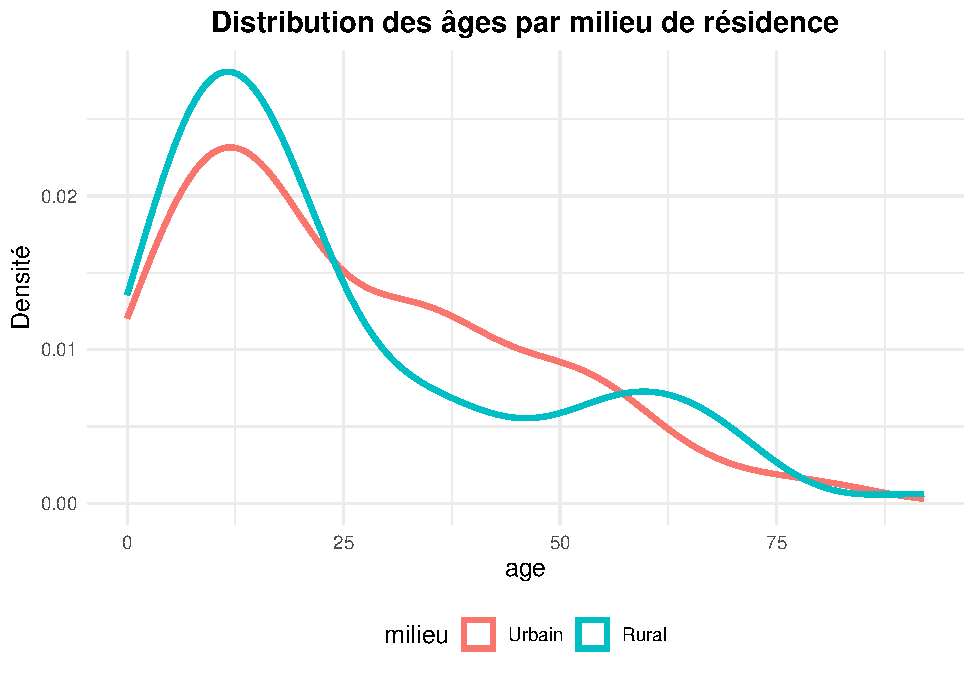
\includegraphics{Stat_non_para_files/figure-latex/unnamed-chunk-101-1.pdf}

\begin{Shaded}
\begin{Highlighting}[]
\FunctionTok{plot\_boxplots}\NormalTok{(sous\_echantillon, }\StringTok{"age"}\NormalTok{, }\StringTok{"milieu"}\NormalTok{, }\StringTok{"Boxplot des âges par milieu de résidence"}\NormalTok{)}
\end{Highlighting}
\end{Shaded}

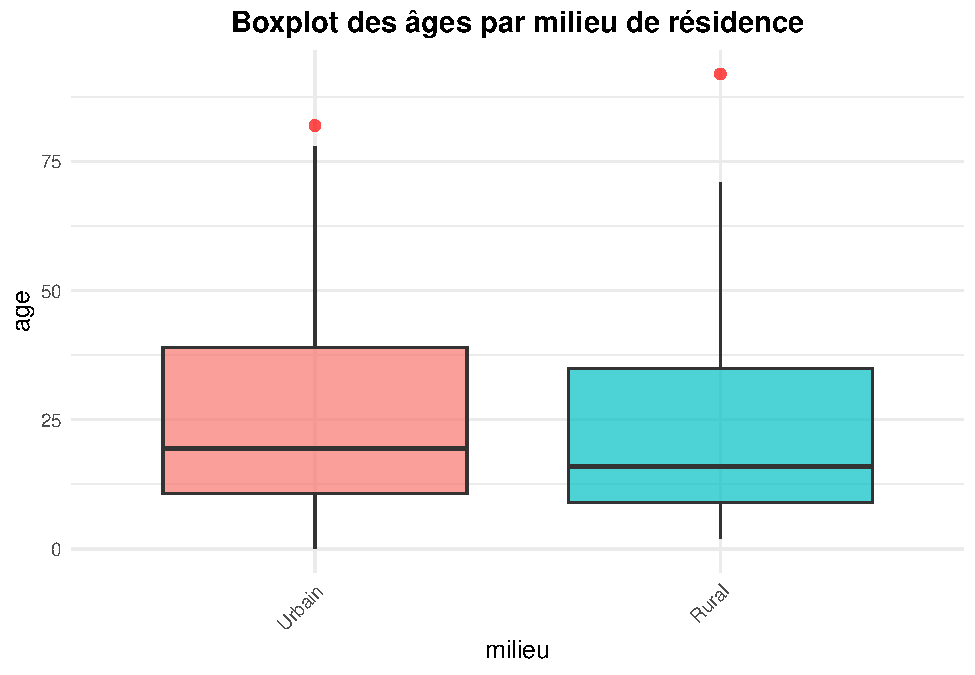
\includegraphics{Stat_non_para_files/figure-latex/unnamed-chunk-102-1.pdf}

\begin{Shaded}
\begin{Highlighting}[]
\FunctionTok{print}\NormalTok{(}\StringTok{"}\SpecialCharTok{\textbackslash{}n}\StringTok{=== TEST DE SAVAGE ==="}\NormalTok{)}
\end{Highlighting}
\end{Shaded}

\begin{verbatim}
## [1] "\n=== TEST DE SAVAGE ==="
\end{verbatim}

\begin{Shaded}
\begin{Highlighting}[]
\NormalTok{resultats }\OtherTok{\textless{}{-}} \FunctionTok{interpretation\_savage}\NormalTok{(sous\_echantillon}\SpecialCharTok{$}\NormalTok{age, sous\_echantillon}\SpecialCharTok{$}\NormalTok{milieu, }
                                 \AttributeTok{alpha =} \FloatTok{0.05}\NormalTok{, }
                                 \AttributeTok{nom\_var\_X =} \StringTok{"Âge"}\NormalTok{, }
                                 \AttributeTok{nom\_var\_Y =} \StringTok{"Milieu de résidence"}\NormalTok{)}
\end{Highlighting}
\end{Shaded}

\begin{verbatim}
## =========================================
##            TEST DE SAVAGE
## =========================================
## 
## Variables analysées:
## - Variable continue: Âge 
## - Variable qualitative: Milieu de résidence 
## 
## Hypothèses:
## H0: Les distributions sont identiques entre les groupes
## H1: Au moins une distribution diffère des autres
## 
## [1] "Nombre d'observations: 200"
## [1] "Nombre de groupes: 2"
## [1] "Effectifs par groupe:"
## Urbain  Rural 
##    100    100 
## Résultats du test:
## - Statistique de test S = 0.0093 
## - Degrés de liberté = 1 
## - P-valeur = 0.9231 
## - Valeur critique (α = 0.05 ) = 3.8415 
## 
## Décision:
## ✗ Non rejet de H0 (p = 0.9231 ≥ α = 0.05 )
## ✗ CONCLUSION: Pas de différence significative entre les distributions.
## 
## Intensité de l'effet:
## → Effet faible ou absent (S ≤ valeur critique)
## 
## =========================================
\end{verbatim}

\subsubsection{Test de Mood}\label{test-de-mood}

\begin{Shaded}
\begin{Highlighting}[]
\CommentTok{\# Données d\textquotesingle{}exemple}
\NormalTok{x3 }\OtherTok{\textless{}{-}} \DecValTok{1}\SpecialCharTok{:}\DecValTok{15}  \CommentTok{\# Les périodes (il y a 15 valeurs dans chaque vecteur)}

\NormalTok{x1 }\OtherTok{\textless{}{-}} \FunctionTok{c}\NormalTok{(}\FloatTok{4.953}\NormalTok{, }\FloatTok{2.524}\NormalTok{, }\FloatTok{2.207}\NormalTok{, }\FloatTok{3.153}\NormalTok{, }\FloatTok{4.637}\NormalTok{, }\FloatTok{4.11}\NormalTok{, }\FloatTok{3.607}\NormalTok{, }\FloatTok{3.91}\NormalTok{, }\FloatTok{3.521}\NormalTok{,  }
        \FloatTok{2.404}\NormalTok{, }\FloatTok{2.112}\NormalTok{, }\FloatTok{6.947}\NormalTok{, }\FloatTok{3.857}\NormalTok{, }\FloatTok{3.756}\NormalTok{, }\FloatTok{4.836}\NormalTok{)  }\CommentTok{\# Groupe A}

\NormalTok{y1 }\OtherTok{\textless{}{-}} \FunctionTok{c}\NormalTok{(}\FloatTok{1.24}\NormalTok{, }\FloatTok{8.163}\NormalTok{, }\FloatTok{3.756}\NormalTok{, }\FloatTok{10.46}\NormalTok{, }\FloatTok{2.172}\NormalTok{, }\FloatTok{4.672}\NormalTok{, }\FloatTok{4.376}\NormalTok{, }\FloatTok{1.002}\NormalTok{, }\FloatTok{1.855}\NormalTok{, }
        \FloatTok{4.227}\NormalTok{, }\FloatTok{3.727}\NormalTok{, }\FloatTok{3.409}\NormalTok{, }\FloatTok{5.973}\NormalTok{, }\FloatTok{5.786}\NormalTok{, }\FloatTok{6.331}\NormalTok{)  }\CommentTok{\# Groupe B}

\CommentTok{\# Tracer la première courbe (x1 en bleu)}
\FunctionTok{plot}\NormalTok{(x3, x1, }\AttributeTok{type =} \StringTok{"l"}\NormalTok{, }\AttributeTok{col =} \StringTok{"blue"}\NormalTok{, }\AttributeTok{lwd =} \DecValTok{2}\NormalTok{, }\AttributeTok{ylim =} \FunctionTok{range}\NormalTok{(}\FunctionTok{c}\NormalTok{(x1, y1)),}
     \AttributeTok{xlab =} \StringTok{"Temps"}\NormalTok{, }\AttributeTok{ylab =} \StringTok{"Valeurs"}\NormalTok{, }\AttributeTok{main =} \StringTok{"Évolution comparée"}\NormalTok{)}

\CommentTok{\# Ajouter la deuxième courbe (y1 en rouge)}
\FunctionTok{lines}\NormalTok{(x3, y1, }\AttributeTok{col =} \StringTok{"red"}\NormalTok{, }\AttributeTok{lwd =} \DecValTok{2}\NormalTok{)}

\CommentTok{\# Ajouter une légende}
\FunctionTok{legend}\NormalTok{(}\StringTok{"topleft"}\NormalTok{, }\AttributeTok{legend =} \FunctionTok{c}\NormalTok{(}\StringTok{"Groupe A"}\NormalTok{, }\StringTok{"Groupe B"}\NormalTok{),}
       \AttributeTok{col =} \FunctionTok{c}\NormalTok{(}\StringTok{"blue"}\NormalTok{, }\StringTok{"red"}\NormalTok{), }\AttributeTok{lty =} \DecValTok{1}\NormalTok{, }\AttributeTok{lwd =} \DecValTok{2}\NormalTok{)}
\end{Highlighting}
\end{Shaded}

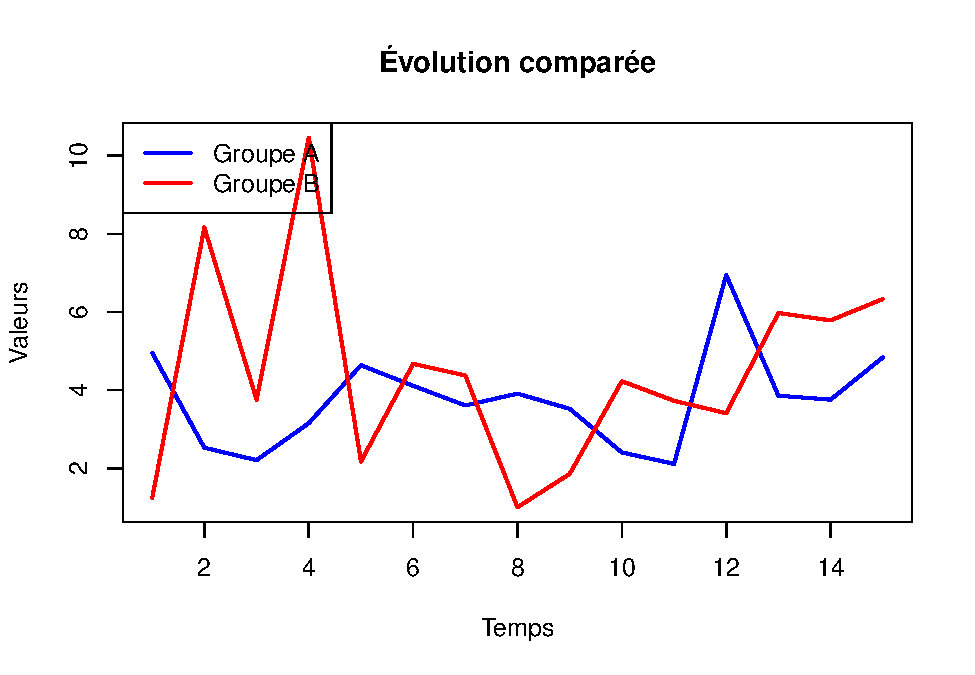
\includegraphics{Stat_non_para_files/figure-latex/unnamed-chunk-104-1.pdf}

\textbf{Création de la base de donneés}

\begin{Shaded}
\begin{Highlighting}[]
\NormalTok{x }\OtherTok{\textless{}{-}} \FunctionTok{c}\NormalTok{(}\FloatTok{4.953}\NormalTok{, }\FloatTok{2.524}\NormalTok{, }\FloatTok{2.207}\NormalTok{, }\FloatTok{3.153}\NormalTok{, }\FloatTok{4.637}\NormalTok{, }\FloatTok{4.11}\NormalTok{, }\FloatTok{3.607}\NormalTok{, }\FloatTok{3.91}\NormalTok{, }\FloatTok{3.521}\NormalTok{,  }\FloatTok{2.404}\NormalTok{, }
       \FloatTok{2.112}\NormalTok{, }\FloatTok{6.947}\NormalTok{, }\FloatTok{3.857}\NormalTok{, }\FloatTok{3.756}\NormalTok{, }\FloatTok{4.836}\NormalTok{)  }\CommentTok{\# Groupe A}
\NormalTok{y }\OtherTok{\textless{}{-}} \FunctionTok{c}\NormalTok{(}\FloatTok{1.24}\NormalTok{, }\FloatTok{8.163}\NormalTok{, }\DecValTok{3}\NormalTok{,}\DecValTok{756}\NormalTok{, }\DecValTok{10}\NormalTok{,}\DecValTok{46}\NormalTok{, }\FloatTok{2.172}\NormalTok{, }\FloatTok{4.672}\NormalTok{, }\FloatTok{4.376}\NormalTok{, }\FloatTok{1.002}\NormalTok{, }\FloatTok{1.855}\NormalTok{, }\FloatTok{4.227}\NormalTok{, }
       \FloatTok{3.727}\NormalTok{, }\FloatTok{3.409}\NormalTok{, }\FloatTok{5.973}\NormalTok{, }\FloatTok{5.786}\NormalTok{, }\FloatTok{6.331}\NormalTok{) }\CommentTok{\# Groupe B}
\end{Highlighting}
\end{Shaded}

\textbf{Appliquer le test de Mood}

\begin{Shaded}
\begin{Highlighting}[]
\FunctionTok{mood.test}\NormalTok{(x, y)}
\end{Highlighting}
\end{Shaded}

\begin{verbatim}
## 
##  Mood two-sample test of scale
## 
## data:  x and y
## Z = -2.3767, p-value = 0.01747
## alternative hypothesis: two.sided
\end{verbatim}

Notre p\_value est inferieur a 0,05 alors on rejet Ho c'est-à-dire que
les dispersions ne sont pas les mêmes. Autrement dit, les dispersions
sont differentes.

A présent, nous allons refaire le test manuellement et comparer aux
résultats précédents, avant d'élaborer une fonction.

\begin{Shaded}
\begin{Highlighting}[]
\NormalTok{n }\OtherTok{\textless{}{-}} \FunctionTok{length}\NormalTok{(x) }\CommentTok{\# taille de X}
\NormalTok{m }\OtherTok{\textless{}{-}} \FunctionTok{length}\NormalTok{(y) }\CommentTok{\# taille de Y}
\NormalTok{N }\OtherTok{\textless{}{-}}\NormalTok{ n }\SpecialCharTok{+}\NormalTok{ m     }\CommentTok{\# taille totale}
\end{Highlighting}
\end{Shaded}

\textbf{Rang, score et tableau}

On combine les deux groupes et on calcule les rangs et les scores

\begin{itemize}
\tightlist
\item
  \textbf{Score de chaque observation}
\end{itemize}

\[
\text{score}_i = \left( \text{rang}_i - \frac{N + 1}{2} \right)^2
\]

\begin{Shaded}
\begin{Highlighting}[]
\CommentTok{\# Combinaison}
\NormalTok{z }\OtherTok{\textless{}{-}} \FunctionTok{c}\NormalTok{(x, y)}
\NormalTok{groupe }\OtherTok{\textless{}{-}} \FunctionTok{c}\NormalTok{(}\FunctionTok{rep}\NormalTok{(}\StringTok{"X"}\NormalTok{, n), }\FunctionTok{rep}\NormalTok{(}\StringTok{"Y"}\NormalTok{, m))}
\NormalTok{rang }\OtherTok{\textless{}{-}} \FunctionTok{rank}\NormalTok{(z)}
\NormalTok{score }\OtherTok{\textless{}{-}}\NormalTok{ (rang }\SpecialCharTok{{-}}\NormalTok{ (N }\SpecialCharTok{+} \DecValTok{1}\NormalTok{) }\SpecialCharTok{/} \DecValTok{2}\NormalTok{)}\SpecialCharTok{\^{}}\DecValTok{2}

\CommentTok{\# Tableau}
\NormalTok{table\_mood }\OtherTok{\textless{}{-}} \FunctionTok{data.frame}\NormalTok{(}\AttributeTok{Observation =}\NormalTok{ z, }\AttributeTok{Groupe =}\NormalTok{ groupe, }\AttributeTok{Rang =}\NormalTok{ rang, }\AttributeTok{Score =}\NormalTok{ score)}
\NormalTok{knitr}\SpecialCharTok{::}\FunctionTok{kable}\NormalTok{(table\_mood, }\AttributeTok{digits =} \DecValTok{3}\NormalTok{)}
\end{Highlighting}
\end{Shaded}

\begin{longtable}[]{@{}rlrr@{}}
\toprule\noalign{}
Observation & Groupe & Rang & Score \\
\midrule\noalign{}
\endhead
\bottomrule\noalign{}
\endlastfoot
4.953 & X & 24 & 56.25 \\
2.524 & X & 8 & 72.25 \\
2.207 & X & 6 & 110.25 \\
3.153 & X & 10 & 42.25 \\
4.637 & X & 21 & 20.25 \\
4.110 & X & 18 & 2.25 \\
3.607 & X & 13 & 12.25 \\
3.910 & X & 17 & 0.25 \\
3.521 & X & 12 & 20.25 \\
2.404 & X & 7 & 90.25 \\
2.112 & X & 4 & 156.25 \\
6.947 & X & 28 & 132.25 \\
3.857 & X & 16 & 0.25 \\
3.756 & X & 15 & 2.25 \\
4.836 & X & 23 & 42.25 \\
1.240 & Y & 2 & 210.25 \\
8.163 & Y & 29 & 156.25 \\
3.000 & Y & 9 & 56.25 \\
756.000 & Y & 32 & 240.25 \\
10.000 & Y & 30 & 182.25 \\
46.000 & Y & 31 & 210.25 \\
2.172 & Y & 5 & 132.25 \\
4.672 & Y & 22 & 30.25 \\
4.376 & Y & 20 & 12.25 \\
1.002 & Y & 1 & 240.25 \\
1.855 & Y & 3 & 182.25 \\
4.227 & Y & 19 & 6.25 \\
3.727 & Y & 14 & 6.25 \\
3.409 & Y & 11 & 30.25 \\
5.973 & Y & 26 & 90.25 \\
5.786 & Y & 25 & 72.25 \\
6.331 & Y & 27 & 110.25 \\
\end{longtable}

\begin{itemize}
\tightlist
\item
  \textbf{On calcule la somme des scores pour le groupe X (appelée
  \(M_n\))}
\end{itemize}

\[
M_n = \sum_{i=1}^n \left( \text{rang}_i - \frac{N + 1}{2} \right)^2
\]

\begin{Shaded}
\begin{Highlighting}[]
\NormalTok{Mn }\OtherTok{\textless{}{-}} \FunctionTok{sum}\NormalTok{(score[groupe }\SpecialCharTok{==} \StringTok{"X"}\NormalTok{])}
\NormalTok{Mn}
\end{Highlighting}
\end{Shaded}

\begin{verbatim}
## [1] 759.75
\end{verbatim}

Ensuite, on calcule l'espérance et la variance.

\begin{itemize}
\tightlist
\item
  \emph{Espérance de \(M_n\)}
\end{itemize}

\[
\mathbb{E}[M_n] = \frac{n (N^2 - 1)}{12}
\]

\begin{itemize}
\tightlist
\item
  \emph{Variance de \(M_n\)}
\end{itemize}

\[
\mathrm{Var}(M_n) = \frac{n m (N + 1)(N^2 - 1)}{180}
\]

\begin{Shaded}
\begin{Highlighting}[]
\NormalTok{esp }\OtherTok{\textless{}{-}}\NormalTok{ n }\SpecialCharTok{*}\NormalTok{ (N}\SpecialCharTok{\^{}}\DecValTok{2} \SpecialCharTok{{-}} \DecValTok{1}\NormalTok{) }\SpecialCharTok{/} \DecValTok{12}
\NormalTok{var }\OtherTok{\textless{}{-}}\NormalTok{ n }\SpecialCharTok{*}\NormalTok{ m }\SpecialCharTok{*}\NormalTok{ (N }\SpecialCharTok{+} \DecValTok{1}\NormalTok{) }\SpecialCharTok{*}\NormalTok{ (N}\SpecialCharTok{\^{}}\DecValTok{2} \SpecialCharTok{{-}} \DecValTok{1}\NormalTok{) }\SpecialCharTok{/} \DecValTok{180}
\NormalTok{esp}
\end{Highlighting}
\end{Shaded}

\begin{verbatim}
## [1] 1278.75
\end{verbatim}

\begin{Shaded}
\begin{Highlighting}[]
\NormalTok{var}
\end{Highlighting}
\end{Shaded}

\begin{verbatim}
## [1] 47825.25
\end{verbatim}

\begin{itemize}
\tightlist
\item
  \textbf{Normalisation : }
\end{itemize}

Statistique normalisée :
\(Z = \frac{M_n - \mathbb{E}[M_n]}{\sqrt{\mathrm{Var}(M_n)}}\)

\begin{Shaded}
\begin{Highlighting}[]
\NormalTok{Z }\OtherTok{\textless{}{-}}\NormalTok{ (Mn }\SpecialCharTok{{-}}\NormalTok{ esp) }\SpecialCharTok{/} \FunctionTok{sqrt}\NormalTok{(var)}
\NormalTok{Z}
\end{Highlighting}
\end{Shaded}

\begin{verbatim}
## [1] -2.373224
\end{verbatim}

\begin{itemize}
\tightlist
\item
  \textbf{Règle de décision : }
\end{itemize}

\(\text{Si } |Z| > z_{1 - \alpha/2}, \text{ alors on rejette } H_0\)

\begin{Shaded}
\begin{Highlighting}[]
\CommentTok{\# Seuil critique}
\NormalTok{  z\_crit }\OtherTok{\textless{}{-}} \FunctionTok{qnorm}\NormalTok{(}\DecValTok{1} \SpecialCharTok{{-}} \FloatTok{0.05} \SpecialCharTok{/} \DecValTok{2}\NormalTok{)}
\NormalTok{z\_crit}
\end{Highlighting}
\end{Shaded}

\begin{verbatim}
## [1] 1.959964
\end{verbatim}

\begin{Shaded}
\begin{Highlighting}[]
\CommentTok{\# calcul du valeur absolue de Z}
\NormalTok{valeur\_Z}\OtherTok{\textless{}{-}} \FunctionTok{abs}\NormalTok{(Z) }
\NormalTok{valeur\_Z}
\end{Highlighting}
\end{Shaded}

\begin{verbatim}
## [1] 2.373224
\end{verbatim}

On voit que la valeur absolue de Z est superieur a 1,96 alors on rejette
Ho c'est a dire les dispersions ne sont pas les mêmes

\textbf{Fonctions}

\begin{Shaded}
\begin{Highlighting}[]
\NormalTok{mood\_test\_manuel }\OtherTok{\textless{}{-}} \ControlFlowTok{function}\NormalTok{(x, y, alpha) \{}
  \CommentTok{\# Étapes préliminaires}
\NormalTok{  n }\OtherTok{\textless{}{-}} \FunctionTok{length}\NormalTok{(x)}
\NormalTok{  m }\OtherTok{\textless{}{-}} \FunctionTok{length}\NormalTok{(y)}
\NormalTok{  N }\OtherTok{\textless{}{-}}\NormalTok{ n }\SpecialCharTok{+}\NormalTok{ m}
\NormalTok{  z }\OtherTok{\textless{}{-}} \FunctionTok{c}\NormalTok{(x, y)}
\NormalTok{  groupe }\OtherTok{\textless{}{-}} \FunctionTok{c}\NormalTok{(}\FunctionTok{rep}\NormalTok{(}\StringTok{"X"}\NormalTok{, n), }\FunctionTok{rep}\NormalTok{(}\StringTok{"Y"}\NormalTok{, m))}
  
  \CommentTok{\# Rangs et scores}
\NormalTok{  rang }\OtherTok{\textless{}{-}} \FunctionTok{rank}\NormalTok{(z)}
\NormalTok{  score }\OtherTok{\textless{}{-}}\NormalTok{ (rang }\SpecialCharTok{{-}}\NormalTok{ (N }\SpecialCharTok{+} \DecValTok{1}\NormalTok{)}\SpecialCharTok{/}\DecValTok{2}\NormalTok{)}\SpecialCharTok{\^{}}\DecValTok{2}
  
  \CommentTok{\# Mn : somme des scores pour le groupe X}
\NormalTok{  Mn }\OtherTok{\textless{}{-}} \FunctionTok{sum}\NormalTok{(score[groupe }\SpecialCharTok{==} \StringTok{"X"}\NormalTok{])}
  
  \CommentTok{\# Espérance et variance de Mn}
\NormalTok{  esperance }\OtherTok{\textless{}{-}}\NormalTok{ n }\SpecialCharTok{*}\NormalTok{ (N}\SpecialCharTok{\^{}}\DecValTok{2} \SpecialCharTok{{-}} \DecValTok{1}\NormalTok{) }\SpecialCharTok{/} \DecValTok{12}
\NormalTok{  variance }\OtherTok{\textless{}{-}}\NormalTok{ n }\SpecialCharTok{*}\NormalTok{ m }\SpecialCharTok{*}\NormalTok{ (N }\SpecialCharTok{+} \DecValTok{1}\NormalTok{) }\SpecialCharTok{*}\NormalTok{ (N}\SpecialCharTok{\^{}}\DecValTok{2} \SpecialCharTok{{-}} \DecValTok{1}\NormalTok{) }\SpecialCharTok{/} \DecValTok{180}
  
  \CommentTok{\# Statistique Z}
\NormalTok{  Z }\OtherTok{\textless{}{-}}\NormalTok{ (Mn }\SpecialCharTok{{-}}\NormalTok{ esperance) }\SpecialCharTok{/} \FunctionTok{sqrt}\NormalTok{(variance)}
\NormalTok{  abs\_Z }\OtherTok{\textless{}{-}} \FunctionTok{abs}\NormalTok{(Z)}
  
  \CommentTok{\# Seuil critique}
\NormalTok{  z\_crit }\OtherTok{\textless{}{-}} \FunctionTok{qnorm}\NormalTok{(}\DecValTok{1} \SpecialCharTok{{-}}\NormalTok{ alpha }\SpecialCharTok{/} \DecValTok{2}\NormalTok{)}
  
  \CommentTok{\# Décision}
\NormalTok{  decision }\OtherTok{\textless{}{-}} \FunctionTok{ifelse}\NormalTok{(abs\_Z }\SpecialCharTok{\textgreater{}}\NormalTok{ z\_crit,}
                     \StringTok{"Rejet de H0 : dispersions différentes"}\NormalTok{,}
                     \StringTok{"On ne rejette pas H0 : dispersions identiques"}\NormalTok{)}
  
  \CommentTok{\# Retourner les résultats sous forme de liste}
\NormalTok{  resultats }\OtherTok{\textless{}{-}} \FunctionTok{list}\NormalTok{(}
    \AttributeTok{Mn =}\NormalTok{ Mn,}
    \AttributeTok{Esperance =}\NormalTok{ esperance,}
    \AttributeTok{Variance =}\NormalTok{ variance,}
    \AttributeTok{Z =}\NormalTok{ Z,}
    \AttributeTok{abs\_Z =}\NormalTok{ abs\_Z,}
    \AttributeTok{z\_critique =}\NormalTok{ z\_crit,}
    \AttributeTok{alpha =}\NormalTok{ alpha,}
    \AttributeTok{Decision =}\NormalTok{ decision}
\NormalTok{  )}
  
  \FunctionTok{return}\NormalTok{(resultats)}
\NormalTok{\}}
\end{Highlighting}
\end{Shaded}

Renseignons à présent les valeurs.

\begin{Shaded}
\begin{Highlighting}[]
\CommentTok{\# Tes données}
\NormalTok{x }\OtherTok{\textless{}{-}} \FunctionTok{c}\NormalTok{(}\FloatTok{4.953}\NormalTok{, }\FloatTok{2.524}\NormalTok{, }\FloatTok{2.207}\NormalTok{, }\FloatTok{3.153}\NormalTok{, }\FloatTok{4.637}\NormalTok{, }\FloatTok{4.11}\NormalTok{, }\FloatTok{3.607}\NormalTok{, }\FloatTok{3.91}\NormalTok{, }\FloatTok{3.521}\NormalTok{,}
       \FloatTok{2.404}\NormalTok{, }\FloatTok{2.112}\NormalTok{, }\FloatTok{6.947}\NormalTok{, }\FloatTok{3.857}\NormalTok{, }\FloatTok{3.756}\NormalTok{, }\FloatTok{4.836}\NormalTok{)}

\NormalTok{y }\OtherTok{\textless{}{-}} \FunctionTok{c}\NormalTok{(}\FloatTok{1.24}\NormalTok{, }\FloatTok{8.163}\NormalTok{, }\FloatTok{3.756}\NormalTok{, }\FloatTok{10.46}\NormalTok{, }\FloatTok{2.172}\NormalTok{, }\FloatTok{4.672}\NormalTok{, }\FloatTok{4.376}\NormalTok{, }\FloatTok{1.002}\NormalTok{, }\FloatTok{1.855}\NormalTok{,}
       \FloatTok{4.227}\NormalTok{, }\FloatTok{3.727}\NormalTok{, }\FloatTok{3.409}\NormalTok{, }\FloatTok{5.973}\NormalTok{, }\FloatTok{5.786}\NormalTok{, }\FloatTok{6.331}\NormalTok{)}

\CommentTok{\# Appel avec alpha = 0.01 (ou tout autre seuil)}
\NormalTok{resultat }\OtherTok{\textless{}{-}} \FunctionTok{mood\_test\_manuel}\NormalTok{(x, y, }\AttributeTok{alpha =} \FloatTok{0.05}\NormalTok{)}

\CommentTok{\# Affichage}
\FunctionTok{print}\NormalTok{(resultat)}
\end{Highlighting}
\end{Shaded}

\begin{verbatim}
## $Mn
## [1] 750.5
## 
## $Esperance
## [1] 1123.75
## 
## $Variance
## [1] 34836.25
## 
## $Z
## [1] -1.999789
## 
## $abs_Z
## [1] 1.999789
## 
## $z_critique
## [1] 1.959964
## 
## $alpha
## [1] 0.05
## 
## $Decision
## [1] "Rejet de H0 : dispersions différentes"
\end{verbatim}

\subsection{Tests d'alternative
générale}\label{tests-dalternative-guxe9nuxe9rale}

\subsubsection{Test de Kolmogorov}\label{test-de-kolmogorov}

\paragraph{Exemple}\label{exemple}

\begin{Shaded}
\begin{Highlighting}[]
\NormalTok{x }\OtherTok{\textless{}{-}} \FunctionTok{c}\NormalTok{(}\FloatTok{0.9}\NormalTok{, }\FloatTok{1.8}\NormalTok{, }\FloatTok{2.2}\NormalTok{, }\FloatTok{2.6}\NormalTok{, }\FloatTok{2.7}\NormalTok{)      }
\NormalTok{y }\OtherTok{\textless{}{-}} \FunctionTok{c}\NormalTok{(}\FloatTok{0.6}\NormalTok{, }\FloatTok{1.1}\NormalTok{, }\FloatTok{1.4}\NormalTok{, }\FloatTok{2.3}\NormalTok{, }\FloatTok{3.0}\NormalTok{, }\FloatTok{3.1}\NormalTok{) }
\end{Highlighting}
\end{Shaded}

\begin{itemize}
\tightlist
\item
  \textbf{Fusion des vecteurs x et y}
\end{itemize}

\begin{Shaded}
\begin{Highlighting}[]
\NormalTok{x\_y }\OtherTok{\textless{}{-}} \FunctionTok{c}\NormalTok{(x,y)}
\NormalTok{x\_yr }\OtherTok{\textless{}{-}} \FunctionTok{sort}\NormalTok{(x\_y)}
\end{Highlighting}
\end{Shaded}

\begin{itemize}
\item
  \textbf{Visualisation des données}

  \begin{itemize}
  \tightlist
  \item
    \textbf{Densité}
  \end{itemize}
\end{itemize}

\begin{Shaded}
\begin{Highlighting}[]
\NormalTok{dx }\OtherTok{\textless{}{-}} \FunctionTok{density}\NormalTok{(x)}
\NormalTok{dy }\OtherTok{\textless{}{-}} \FunctionTok{density}\NormalTok{(y)}

\FunctionTok{plot}\NormalTok{(dx, }\AttributeTok{col =} \StringTok{"blue"}\NormalTok{, }\AttributeTok{lwd =} \DecValTok{2}\NormalTok{, }\AttributeTok{main =} \StringTok{"Estimation des densités"}\NormalTok{, }\AttributeTok{xlab =} \StringTok{"Valeurs"}\NormalTok{, }\AttributeTok{ylim =} \FunctionTok{range}\NormalTok{(}\DecValTok{0}\NormalTok{, dx}\SpecialCharTok{$}\NormalTok{y, dy}\SpecialCharTok{$}\NormalTok{y))}
\FunctionTok{lines}\NormalTok{(dy, }\AttributeTok{col =} \StringTok{"red"}\NormalTok{, }\AttributeTok{lwd =} \DecValTok{2}\NormalTok{)}

\FunctionTok{legend}\NormalTok{(}\StringTok{"topright"}\NormalTok{, }\AttributeTok{legend =} \FunctionTok{c}\NormalTok{(}\StringTok{"Fx"}\NormalTok{, }\StringTok{"Fy"}\NormalTok{), }\AttributeTok{col =} \FunctionTok{c}\NormalTok{(}\StringTok{"blue"}\NormalTok{, }\StringTok{"red"}\NormalTok{), }\AttributeTok{lwd =} \DecValTok{2}\NormalTok{)}
\end{Highlighting}
\end{Shaded}

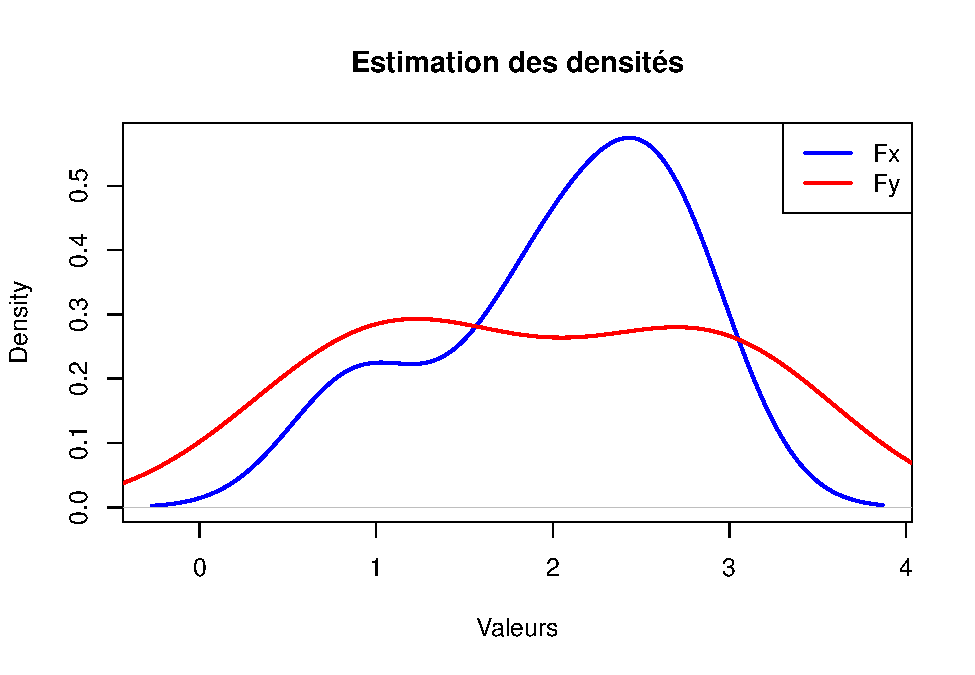
\includegraphics{Stat_non_para_files/figure-latex/unnamed-chunk-118-1.pdf}

\begin{itemize}
\tightlist
\item
  \textbf{Fonction de répartition empirique}
\end{itemize}

\begin{Shaded}
\begin{Highlighting}[]
\NormalTok{Fx }\OtherTok{\textless{}{-}} \FunctionTok{ecdf}\NormalTok{(x)}
\NormalTok{Fy }\OtherTok{\textless{}{-}} \FunctionTok{ecdf}\NormalTok{(y)}

\NormalTok{range\_x }\OtherTok{\textless{}{-}} \FunctionTok{seq}\NormalTok{(}\FunctionTok{min}\NormalTok{(x\_yr) }\SpecialCharTok{{-}} \FloatTok{0.1}\NormalTok{, }\FunctionTok{max}\NormalTok{(x\_yr) }\SpecialCharTok{+} \FloatTok{0.1}\NormalTok{, }\AttributeTok{length.out =} \DecValTok{100}\NormalTok{)}

\FunctionTok{plot}\NormalTok{(range\_x, }\FunctionTok{Fx}\NormalTok{(range\_x), }\AttributeTok{type =} \StringTok{"s"}\NormalTok{, }\AttributeTok{col =} \StringTok{"blue"}\NormalTok{, }\AttributeTok{lwd =} \DecValTok{2}\NormalTok{,}
     \AttributeTok{xlab =} \StringTok{"Valeurs"}\NormalTok{, }\AttributeTok{ylab =} \StringTok{"F(x)"}\NormalTok{, }\AttributeTok{main =} \StringTok{"Fonctions de répartition empiriques"}\NormalTok{)}
\FunctionTok{lines}\NormalTok{(range\_x, }\FunctionTok{Fy}\NormalTok{(range\_x), }\AttributeTok{type =} \StringTok{"s"}\NormalTok{, }\AttributeTok{col =} \StringTok{"red"}\NormalTok{, }\AttributeTok{lwd =} \DecValTok{2}\NormalTok{)}

\FunctionTok{legend}\NormalTok{(}\StringTok{"topright"}\NormalTok{, }\AttributeTok{legend =} \FunctionTok{c}\NormalTok{(}\StringTok{"Fx (x)"}\NormalTok{, }\StringTok{"Fy (x)"}\NormalTok{), }\AttributeTok{col =} \FunctionTok{c}\NormalTok{(}\StringTok{"blue"}\NormalTok{, }\StringTok{"red"}\NormalTok{), }\AttributeTok{lwd =} \DecValTok{2}\NormalTok{)}
\end{Highlighting}
\end{Shaded}

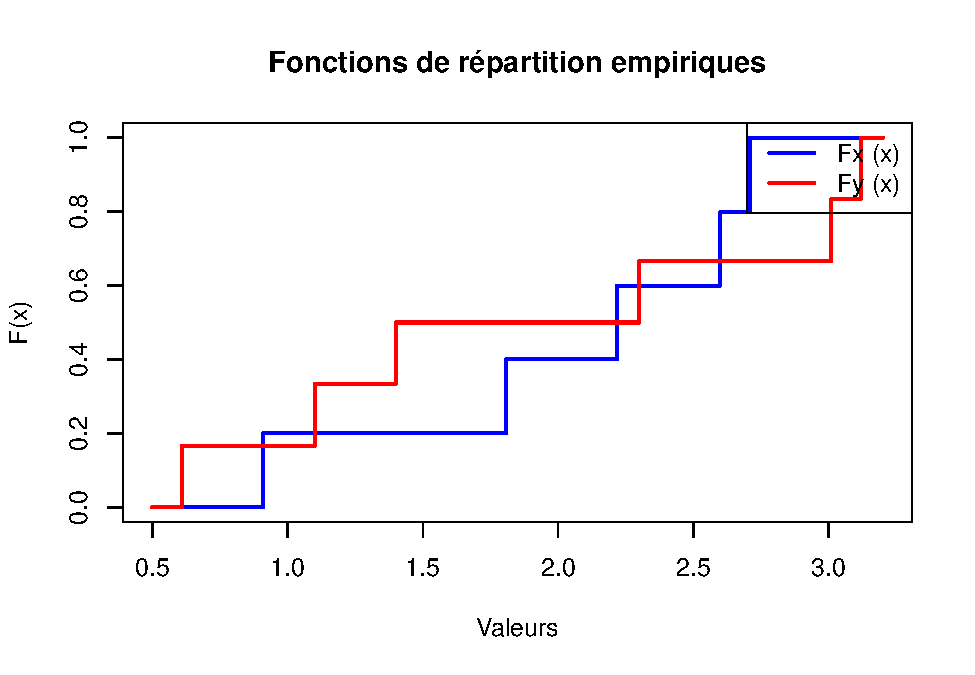
\includegraphics{Stat_non_para_files/figure-latex/unnamed-chunk-119-1.pdf}

\begin{itemize}
\tightlist
\item
  \textbf{Tableau format long}
\end{itemize}

\begin{Shaded}
\begin{Highlighting}[]
\NormalTok{N }\OtherTok{\textless{}{-}} \FunctionTok{length}\NormalTok{(x\_yr)}
\NormalTok{x\_long }\OtherTok{\textless{}{-}} \FunctionTok{c}\NormalTok{(x, }\FunctionTok{rep}\NormalTok{(}\ConstantTok{NA}\NormalTok{, N }\SpecialCharTok{{-}} \FunctionTok{length}\NormalTok{(x)))}
\NormalTok{y\_long }\OtherTok{\textless{}{-}} \FunctionTok{c}\NormalTok{(y, }\FunctionTok{rep}\NormalTok{(}\ConstantTok{NA}\NormalTok{, N }\SpecialCharTok{{-}} \FunctionTok{length}\NormalTok{(y)))}
\NormalTok{df }\OtherTok{\textless{}{-}} \FunctionTok{data.frame}\NormalTok{(}\AttributeTok{x =}\NormalTok{ x\_long, }\AttributeTok{y =}\NormalTok{ y\_long)}

\NormalTok{df}\SpecialCharTok{$}\NormalTok{x\_y }\OtherTok{\textless{}{-}}\NormalTok{ x\_yr}

\CommentTok{\# Serie source de chaque valeur}
\NormalTok{df}\SpecialCharTok{$}\NormalTok{xn }\OtherTok{\textless{}{-}} \FunctionTok{ifelse}\NormalTok{(df}\SpecialCharTok{$}\NormalTok{x\_y }\SpecialCharTok{\%in\%}\NormalTok{ x, }\DecValTok{1}\NormalTok{, }\DecValTok{0}\NormalTok{)}
\NormalTok{df}\SpecialCharTok{$}\NormalTok{yn }\OtherTok{\textless{}{-}} \FunctionTok{ifelse}\NormalTok{(df}\SpecialCharTok{$}\NormalTok{x\_y }\SpecialCharTok{\%in\%}\NormalTok{ y, }\DecValTok{1}\NormalTok{, }\DecValTok{0}\NormalTok{)}

\CommentTok{\# Effectifs cumulés}
\NormalTok{df}\SpecialCharTok{$}\NormalTok{ECC1 }\OtherTok{\textless{}{-}} \FunctionTok{sapply}\NormalTok{(df}\SpecialCharTok{$}\NormalTok{x\_y, }\ControlFlowTok{function}\NormalTok{(val) \{}
  \FunctionTok{sum}\NormalTok{(x }\SpecialCharTok{\textless{}=}\NormalTok{ val)}
\NormalTok{\})}
\NormalTok{df}\SpecialCharTok{$}\NormalTok{ECC2 }\OtherTok{\textless{}{-}} \FunctionTok{sapply}\NormalTok{(df}\SpecialCharTok{$}\NormalTok{x\_y, }\ControlFlowTok{function}\NormalTok{(val) \{}
  \FunctionTok{sum}\NormalTok{(y }\SpecialCharTok{\textless{}=}\NormalTok{ val)}
\NormalTok{\})}

\CommentTok{\# Fonction de répartition}
\NormalTok{df}\SpecialCharTok{$}\NormalTok{Fx }\OtherTok{\textless{}{-}}\NormalTok{ df}\SpecialCharTok{$}\NormalTok{ECC1}\SpecialCharTok{/}\FunctionTok{length}\NormalTok{(x)}
\NormalTok{df}\SpecialCharTok{$}\NormalTok{Fy }\OtherTok{\textless{}{-}}\NormalTok{ df}\SpecialCharTok{$}\NormalTok{ECC2}\SpecialCharTok{/}\FunctionTok{length}\NormalTok{(y)}

\NormalTok{df[}\StringTok{"Fx{-}Fy"}\NormalTok{] }\OtherTok{\textless{}{-}}\NormalTok{ df}\SpecialCharTok{$}\NormalTok{Fx}\SpecialCharTok{{-}}\NormalTok{df}\SpecialCharTok{$}\NormalTok{Fy}
\NormalTok{df[}\StringTok{"Fy{-}Fx"}\NormalTok{] }\OtherTok{\textless{}{-}}\NormalTok{ df}\SpecialCharTok{$}\NormalTok{Fy}\SpecialCharTok{{-}}\NormalTok{df}\SpecialCharTok{$}\NormalTok{Fx}

\FunctionTok{print}\NormalTok{(df)}
\end{Highlighting}
\end{Shaded}

\begin{verbatim}
##      x   y x_y xn yn ECC1 ECC2  Fx        Fy       Fx-Fy       Fy-Fx
## 1  0.9 0.6 0.6  0  1    0    1 0.0 0.1666667 -0.16666667  0.16666667
## 2  1.8 1.1 0.9  1  0    1    1 0.2 0.1666667  0.03333333 -0.03333333
## 3  2.2 1.4 1.1  0  1    1    2 0.2 0.3333333 -0.13333333  0.13333333
## 4  2.6 2.3 1.4  0  1    1    3 0.2 0.5000000 -0.30000000  0.30000000
## 5  2.7 3.0 1.8  1  0    2    3 0.4 0.5000000 -0.10000000  0.10000000
## 6   NA 3.1 2.2  1  0    3    3 0.6 0.5000000  0.10000000 -0.10000000
## 7   NA  NA 2.3  0  1    3    4 0.6 0.6666667 -0.06666667  0.06666667
## 8   NA  NA 2.6  1  0    4    4 0.8 0.6666667  0.13333333 -0.13333333
## 9   NA  NA 2.7  1  0    5    4 1.0 0.6666667  0.33333333 -0.33333333
## 10  NA  NA 3.0  0  1    5    5 1.0 0.8333333  0.16666667 -0.16666667
## 11  NA  NA 3.1  0  1    5    6 1.0 1.0000000  0.00000000  0.00000000
\end{verbatim}

\begin{itemize}
\tightlist
\item
  \textbf{Statistique de test}
\end{itemize}

La table de Kolmogrov n'est pas tabulé sur R.

\begin{Shaded}
\begin{Highlighting}[]
\NormalTok{Kmn }\OtherTok{\textless{}{-}} \FunctionTok{max}\NormalTok{(df[}\StringTok{"Fx{-}Fy"}\NormalTok{],df[}\StringTok{"Fy{-}Fx"}\NormalTok{])}
\FunctionTok{paste}\NormalTok{(}\StringTok{"Kmn = "}\NormalTok{, Kmn)}
\end{Highlighting}
\end{Shaded}

\begin{verbatim}
## [1] "Kmn =  0.333333333333333"
\end{verbatim}

\begin{Shaded}
\begin{Highlighting}[]
\FunctionTok{paste}\NormalTok{(}\StringTok{"Valeur de c avec la loi normale standard"}\NormalTok{, }\FunctionTok{pnorm}\NormalTok{(}\FloatTok{0.975}\NormalTok{, }\AttributeTok{mean =} \DecValTok{0}\NormalTok{, }\AttributeTok{sd =} \DecValTok{1}\NormalTok{)}
\NormalTok{)}
\end{Highlighting}
\end{Shaded}

\begin{verbatim}
## [1] "Valeur de c avec la loi normale standard 0.83521987001969"
\end{verbatim}

\begin{Shaded}
\begin{Highlighting}[]
\FunctionTok{paste}\NormalTok{(}\StringTok{"Test de Kolmogrov sur R"}\NormalTok{)}
\end{Highlighting}
\end{Shaded}

\begin{verbatim}
## [1] "Test de Kolmogrov sur R"
\end{verbatim}

\begin{Shaded}
\begin{Highlighting}[]
\FunctionTok{print}\NormalTok{(}\FunctionTok{ks.test}\NormalTok{(x, y))}
\end{Highlighting}
\end{Shaded}

\begin{verbatim}
## 
##  Exact two-sample Kolmogorov-Smirnov test
## 
## data:  x and y
## D = 0.33333, p-value = 0.8182
## alternative hypothesis: two-sided
\end{verbatim}

\paragraph{Fonctions}\label{fonctions}

\begin{Shaded}
\begin{Highlighting}[]
\NormalTok{ks.stat }\OtherTok{\textless{}{-}} \ControlFlowTok{function}\NormalTok{(x, y) \{}
\NormalTok{  x\_yr }\OtherTok{\textless{}{-}} \FunctionTok{sort}\NormalTok{(}\FunctionTok{c}\NormalTok{(x, y))}
\NormalTok{  N }\OtherTok{\textless{}{-}} \FunctionTok{length}\NormalTok{(x\_yr)}
  
\NormalTok{  x\_long }\OtherTok{\textless{}{-}} \FunctionTok{c}\NormalTok{(x, }\FunctionTok{rep}\NormalTok{(}\ConstantTok{NA}\NormalTok{, N }\SpecialCharTok{{-}} \FunctionTok{length}\NormalTok{(x)))}
\NormalTok{  y\_long }\OtherTok{\textless{}{-}} \FunctionTok{c}\NormalTok{(y, }\FunctionTok{rep}\NormalTok{(}\ConstantTok{NA}\NormalTok{, N }\SpecialCharTok{{-}} \FunctionTok{length}\NormalTok{(y)))}
  
  \CommentTok{\# Créer le tableau initial}
\NormalTok{  df }\OtherTok{\textless{}{-}} \FunctionTok{data.frame}\NormalTok{(}
    \AttributeTok{x =}\NormalTok{ x\_long,}
    \AttributeTok{y =}\NormalTok{ y\_long,}
    \AttributeTok{x\_y =}\NormalTok{ x\_yr}
\NormalTok{  )}
  
\NormalTok{  df}\SpecialCharTok{$}\NormalTok{xn }\OtherTok{\textless{}{-}} \FunctionTok{ifelse}\NormalTok{(df}\SpecialCharTok{$}\NormalTok{x\_y }\SpecialCharTok{\%in\%}\NormalTok{ x, }\DecValTok{1}\NormalTok{, }\DecValTok{0}\NormalTok{)}
\NormalTok{  df}\SpecialCharTok{$}\NormalTok{yn }\OtherTok{\textless{}{-}} \FunctionTok{ifelse}\NormalTok{(df}\SpecialCharTok{$}\NormalTok{x\_y }\SpecialCharTok{\%in\%}\NormalTok{ y, }\DecValTok{1}\NormalTok{, }\DecValTok{0}\NormalTok{)}
  
  \CommentTok{\# Effectifs cumulés pour chaque valeur de x\_y}
\NormalTok{  df}\SpecialCharTok{$}\NormalTok{ECC1 }\OtherTok{\textless{}{-}} \FunctionTok{sapply}\NormalTok{(df}\SpecialCharTok{$}\NormalTok{x\_y, }\ControlFlowTok{function}\NormalTok{(val) }\FunctionTok{sum}\NormalTok{(x }\SpecialCharTok{\textless{}=}\NormalTok{ val))}
\NormalTok{  df}\SpecialCharTok{$}\NormalTok{ECC2 }\OtherTok{\textless{}{-}} \FunctionTok{sapply}\NormalTok{(df}\SpecialCharTok{$}\NormalTok{x\_y, }\ControlFlowTok{function}\NormalTok{(val) }\FunctionTok{sum}\NormalTok{(y }\SpecialCharTok{\textless{}=}\NormalTok{ val))}
  
  \CommentTok{\# Fonctions de répartition empiriques}
\NormalTok{  df}\SpecialCharTok{$}\NormalTok{Fx }\OtherTok{\textless{}{-}}\NormalTok{ df}\SpecialCharTok{$}\NormalTok{ECC1 }\SpecialCharTok{/} \FunctionTok{length}\NormalTok{(x)}
\NormalTok{  df}\SpecialCharTok{$}\NormalTok{Fy }\OtherTok{\textless{}{-}}\NormalTok{ df}\SpecialCharTok{$}\NormalTok{ECC2 }\SpecialCharTok{/} \FunctionTok{length}\NormalTok{(y)}
  
\NormalTok{  df[}\StringTok{"Fx{-}Fy"}\NormalTok{] }\OtherTok{\textless{}{-}}\NormalTok{ df}\SpecialCharTok{$}\NormalTok{Fx }\SpecialCharTok{{-}}\NormalTok{ df}\SpecialCharTok{$}\NormalTok{Fy}
\NormalTok{  df[}\StringTok{"Fy{-}Fx"}\NormalTok{] }\OtherTok{\textless{}{-}}\NormalTok{ df}\SpecialCharTok{$}\NormalTok{Fy }\SpecialCharTok{{-}}\NormalTok{ df}\SpecialCharTok{$}\NormalTok{Fx}
  
  \CommentTok{\# Statistique de test}
\NormalTok{  Kmn }\OtherTok{\textless{}{-}} \FunctionTok{max}\NormalTok{(df[}\StringTok{"Fx{-}Fy"}\NormalTok{],df[}\StringTok{"Fy{-}Fx"}\NormalTok{])}
  
  \FunctionTok{return}\NormalTok{(}\FunctionTok{list}\NormalTok{(}
    \AttributeTok{tableau =}\NormalTok{ df,}
    \AttributeTok{Kmn =}\NormalTok{ Kmn}
\NormalTok{  ))}
\NormalTok{\}}
\end{Highlighting}
\end{Shaded}

\paragraph{Application}\label{application-1}

\begin{Shaded}
\begin{Highlighting}[]
\NormalTok{df }\OtherTok{\textless{}{-}} \FunctionTok{read\_excel}\NormalTok{(}\StringTok{"BASES}\SpecialCharTok{\textbackslash{}\textbackslash{}}\StringTok{notes\_kolmogorov.xlsx"}\NormalTok{)}

\NormalTok{x }\OtherTok{\textless{}{-}}\NormalTok{ df[[}\StringTok{"Anthropo/Moyenne"}\NormalTok{]]}
\NormalTok{y }\OtherTok{\textless{}{-}}\NormalTok{ df[[}\StringTok{"Estimation/Moyenne"}\NormalTok{]]}

\FunctionTok{ks.stat}\NormalTok{(x,y)}
\end{Highlighting}
\end{Shaded}

\begin{verbatim}
## $tableau
##       x    y  x_y xn yn ECC1 ECC2         Fx        Fy      Fx-Fy     Fy-Fx
## 1  16.5  8.0  8.0  1  1    1   13 0.02380952 0.3095238 -0.2857143 0.2857143
## 2  14.5 13.0  8.0  1  1    1   13 0.02380952 0.3095238 -0.2857143 0.2857143
## 3  15.5  8.0  8.0  1  1    1   13 0.02380952 0.3095238 -0.2857143 0.2857143
## 4   8.0 10.0  8.0  1  1    1   13 0.02380952 0.3095238 -0.2857143 0.2857143
## 5  15.0 10.0  8.0  1  1    1   13 0.02380952 0.3095238 -0.2857143 0.2857143
## 6  15.0  8.5  8.0  1  1    1   13 0.02380952 0.3095238 -0.2857143 0.2857143
## 7  15.5  9.5  8.0  1  1    1   13 0.02380952 0.3095238 -0.2857143 0.2857143
## 8  16.0 10.5  8.0  1  1    1   13 0.02380952 0.3095238 -0.2857143 0.2857143
## 9  14.5 10.5  8.0  1  1    1   13 0.02380952 0.3095238 -0.2857143 0.2857143
## 10 15.5  8.0  8.0  1  1    1   13 0.02380952 0.3095238 -0.2857143 0.2857143
## 11 16.5 10.0  8.0  1  1    1   13 0.02380952 0.3095238 -0.2857143 0.2857143
## 12 14.0 10.0  8.0  1  1    1   13 0.02380952 0.3095238 -0.2857143 0.2857143
## 13 14.5 13.5  8.0  1  1    1   13 0.02380952 0.3095238 -0.2857143 0.2857143
## 14 15.5  8.0  8.0  1  1    1   13 0.02380952 0.3095238 -0.2857143 0.2857143
## 15 16.0 11.5  8.5  0  1    1   15 0.02380952 0.3571429 -0.3333333 0.3333333
## 16 16.0  8.0  8.5  0  1    1   15 0.02380952 0.3571429 -0.3333333 0.3333333
## 17 16.5  8.0  9.5  0  1    1   17 0.02380952 0.4047619 -0.3809524 0.3809524
## 18 16.0 10.0  9.5  0  1    1   17 0.02380952 0.4047619 -0.3809524 0.3809524
## 19 15.5 13.5 10.0  0  1    1   25 0.02380952 0.5952381 -0.5714286 0.5714286
## 20 16.0 11.0 10.0  0  1    1   25 0.02380952 0.5952381 -0.5714286 0.5714286
## 21 16.5 12.0 10.0  0  1    1   25 0.02380952 0.5952381 -0.5714286 0.5714286
## 22 14.5  8.0 10.0  0  1    1   25 0.02380952 0.5952381 -0.5714286 0.5714286
## 23 16.5 11.0 10.0  0  1    1   25 0.02380952 0.5952381 -0.5714286 0.5714286
## 24 15.5  8.0 10.0  0  1    1   25 0.02380952 0.5952381 -0.5714286 0.5714286
## 25 15.5  8.0 10.0  0  1    1   25 0.02380952 0.5952381 -0.5714286 0.5714286
## 26 15.0 11.0 10.0  0  1    1   25 0.02380952 0.5952381 -0.5714286 0.5714286
## 27 14.5  8.0 10.5  0  1    1   29 0.02380952 0.6904762 -0.6666667 0.6666667
## 28 14.5 10.0 10.5  0  1    1   29 0.02380952 0.6904762 -0.6666667 0.6666667
## 29 16.0 10.0 10.5  0  1    1   29 0.02380952 0.6904762 -0.6666667 0.6666667
## 30 14.5  8.0 10.5  0  1    1   29 0.02380952 0.6904762 -0.6666667 0.6666667
## 31 15.0 10.5 11.0  0  1    1   32 0.02380952 0.7619048 -0.7380952 0.7380952
## 32 16.0 14.0 11.0  0  1    1   32 0.02380952 0.7619048 -0.7380952 0.7380952
## 33 16.5 10.0 11.0  0  1    1   32 0.02380952 0.7619048 -0.7380952 0.7380952
## 34 15.5  8.0 11.5  0  1    1   34 0.02380952 0.8095238 -0.7857143 0.7857143
## 35 15.5 10.5 11.5  0  1    1   34 0.02380952 0.8095238 -0.7857143 0.7857143
## 36 16.0 12.5 12.0  0  1    1   35 0.02380952 0.8333333 -0.8095238 0.8095238
## 37 15.0 12.5 12.5  0  1    1   38 0.02380952 0.9047619 -0.8809524 0.8809524
## 38 15.5  8.5 12.5  0  1    1   38 0.02380952 0.9047619 -0.8809524 0.8809524
## 39 16.5 12.5 12.5  0  1    1   38 0.02380952 0.9047619 -0.8809524 0.8809524
## 40 16.5  8.0 13.0  0  1    1   39 0.02380952 0.9285714 -0.9047619 0.9047619
## 41 15.0  9.5 13.5  0  1    1   41 0.02380952 0.9761905 -0.9523810 0.9523810
## 42 16.0 11.5 13.5  0  1    1   41 0.02380952 0.9761905 -0.9523810 0.9523810
## 43   NA   NA 14.0  1  1    2   42 0.04761905 1.0000000 -0.9523810 0.9523810
## 44   NA   NA 14.0  1  1    2   42 0.04761905 1.0000000 -0.9523810 0.9523810
## 45   NA   NA 14.5  1  0    9   42 0.21428571 1.0000000 -0.7857143 0.7857143
## 46   NA   NA 14.5  1  0    9   42 0.21428571 1.0000000 -0.7857143 0.7857143
## 47   NA   NA 14.5  1  0    9   42 0.21428571 1.0000000 -0.7857143 0.7857143
## 48   NA   NA 14.5  1  0    9   42 0.21428571 1.0000000 -0.7857143 0.7857143
## 49   NA   NA 14.5  1  0    9   42 0.21428571 1.0000000 -0.7857143 0.7857143
## 50   NA   NA 14.5  1  0    9   42 0.21428571 1.0000000 -0.7857143 0.7857143
## 51   NA   NA 14.5  1  0    9   42 0.21428571 1.0000000 -0.7857143 0.7857143
## 52   NA   NA 15.0  1  0   15   42 0.35714286 1.0000000 -0.6428571 0.6428571
## 53   NA   NA 15.0  1  0   15   42 0.35714286 1.0000000 -0.6428571 0.6428571
## 54   NA   NA 15.0  1  0   15   42 0.35714286 1.0000000 -0.6428571 0.6428571
## 55   NA   NA 15.0  1  0   15   42 0.35714286 1.0000000 -0.6428571 0.6428571
## 56   NA   NA 15.0  1  0   15   42 0.35714286 1.0000000 -0.6428571 0.6428571
## 57   NA   NA 15.0  1  0   15   42 0.35714286 1.0000000 -0.6428571 0.6428571
## 58   NA   NA 15.5  1  0   25   42 0.59523810 1.0000000 -0.4047619 0.4047619
## 59   NA   NA 15.5  1  0   25   42 0.59523810 1.0000000 -0.4047619 0.4047619
## 60   NA   NA 15.5  1  0   25   42 0.59523810 1.0000000 -0.4047619 0.4047619
## 61   NA   NA 15.5  1  0   25   42 0.59523810 1.0000000 -0.4047619 0.4047619
## 62   NA   NA 15.5  1  0   25   42 0.59523810 1.0000000 -0.4047619 0.4047619
## 63   NA   NA 15.5  1  0   25   42 0.59523810 1.0000000 -0.4047619 0.4047619
## 64   NA   NA 15.5  1  0   25   42 0.59523810 1.0000000 -0.4047619 0.4047619
## 65   NA   NA 15.5  1  0   25   42 0.59523810 1.0000000 -0.4047619 0.4047619
## 66   NA   NA 15.5  1  0   25   42 0.59523810 1.0000000 -0.4047619 0.4047619
## 67   NA   NA 15.5  1  0   25   42 0.59523810 1.0000000 -0.4047619 0.4047619
## 68   NA   NA 16.0  1  0   34   42 0.80952381 1.0000000 -0.1904762 0.1904762
## 69   NA   NA 16.0  1  0   34   42 0.80952381 1.0000000 -0.1904762 0.1904762
## 70   NA   NA 16.0  1  0   34   42 0.80952381 1.0000000 -0.1904762 0.1904762
## 71   NA   NA 16.0  1  0   34   42 0.80952381 1.0000000 -0.1904762 0.1904762
## 72   NA   NA 16.0  1  0   34   42 0.80952381 1.0000000 -0.1904762 0.1904762
## 73   NA   NA 16.0  1  0   34   42 0.80952381 1.0000000 -0.1904762 0.1904762
## 74   NA   NA 16.0  1  0   34   42 0.80952381 1.0000000 -0.1904762 0.1904762
## 75   NA   NA 16.0  1  0   34   42 0.80952381 1.0000000 -0.1904762 0.1904762
## 76   NA   NA 16.0  1  0   34   42 0.80952381 1.0000000 -0.1904762 0.1904762
## 77   NA   NA 16.5  1  0   42   42 1.00000000 1.0000000  0.0000000 0.0000000
## 78   NA   NA 16.5  1  0   42   42 1.00000000 1.0000000  0.0000000 0.0000000
## 79   NA   NA 16.5  1  0   42   42 1.00000000 1.0000000  0.0000000 0.0000000
## 80   NA   NA 16.5  1  0   42   42 1.00000000 1.0000000  0.0000000 0.0000000
## 81   NA   NA 16.5  1  0   42   42 1.00000000 1.0000000  0.0000000 0.0000000
## 82   NA   NA 16.5  1  0   42   42 1.00000000 1.0000000  0.0000000 0.0000000
## 83   NA   NA 16.5  1  0   42   42 1.00000000 1.0000000  0.0000000 0.0000000
## 84   NA   NA 16.5  1  0   42   42 1.00000000 1.0000000  0.0000000 0.0000000
## 
## $Kmn
## [1] 0.952381
\end{verbatim}

\begin{Shaded}
\begin{Highlighting}[]
\FunctionTok{ks.test}\NormalTok{(x, y)}
\end{Highlighting}
\end{Shaded}

\begin{verbatim}
## 
##  Exact two-sample Kolmogorov-Smirnov test
## 
## data:  x and y
## D = 0.95238, p-value < 2.2e-16
## alternative hypothesis: two-sided
\end{verbatim}

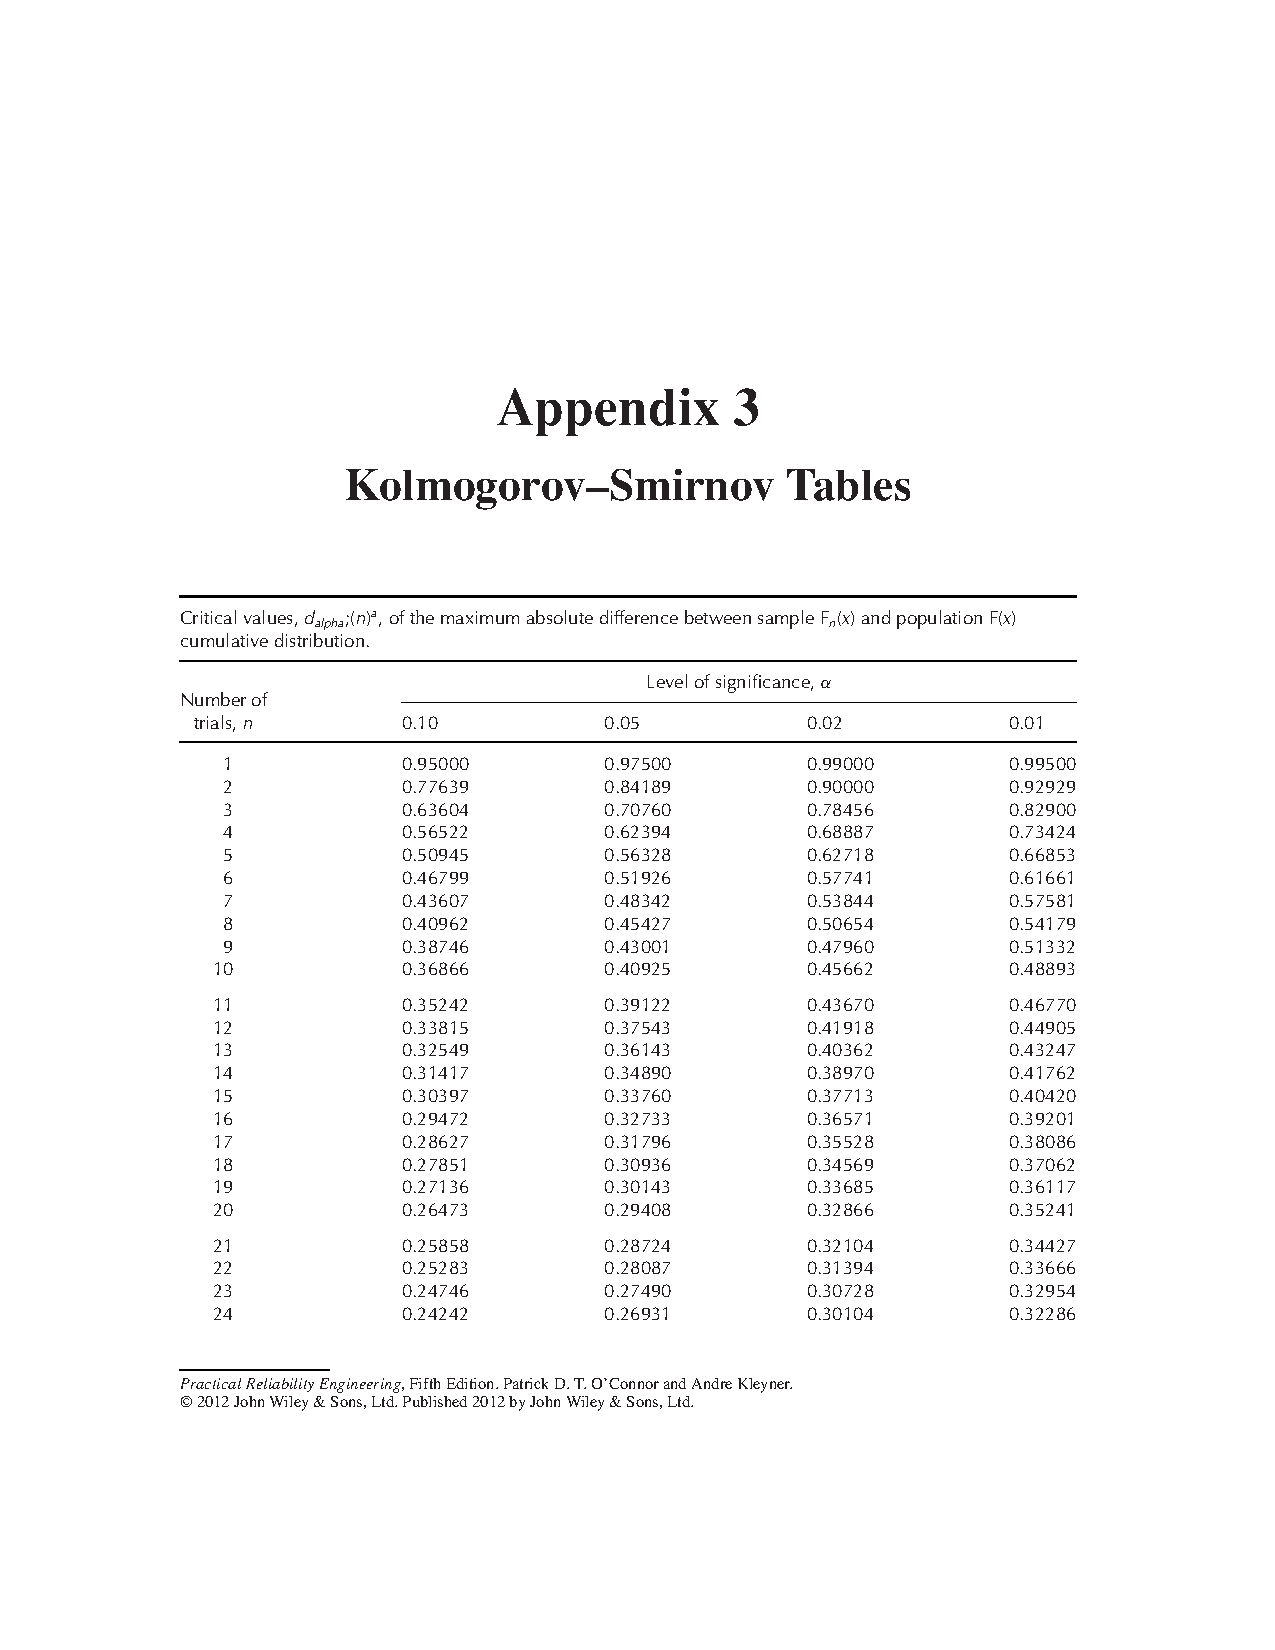
\includepdf{TABLE_KOLMOGOROV_SMIRNOV_1.pdf} 
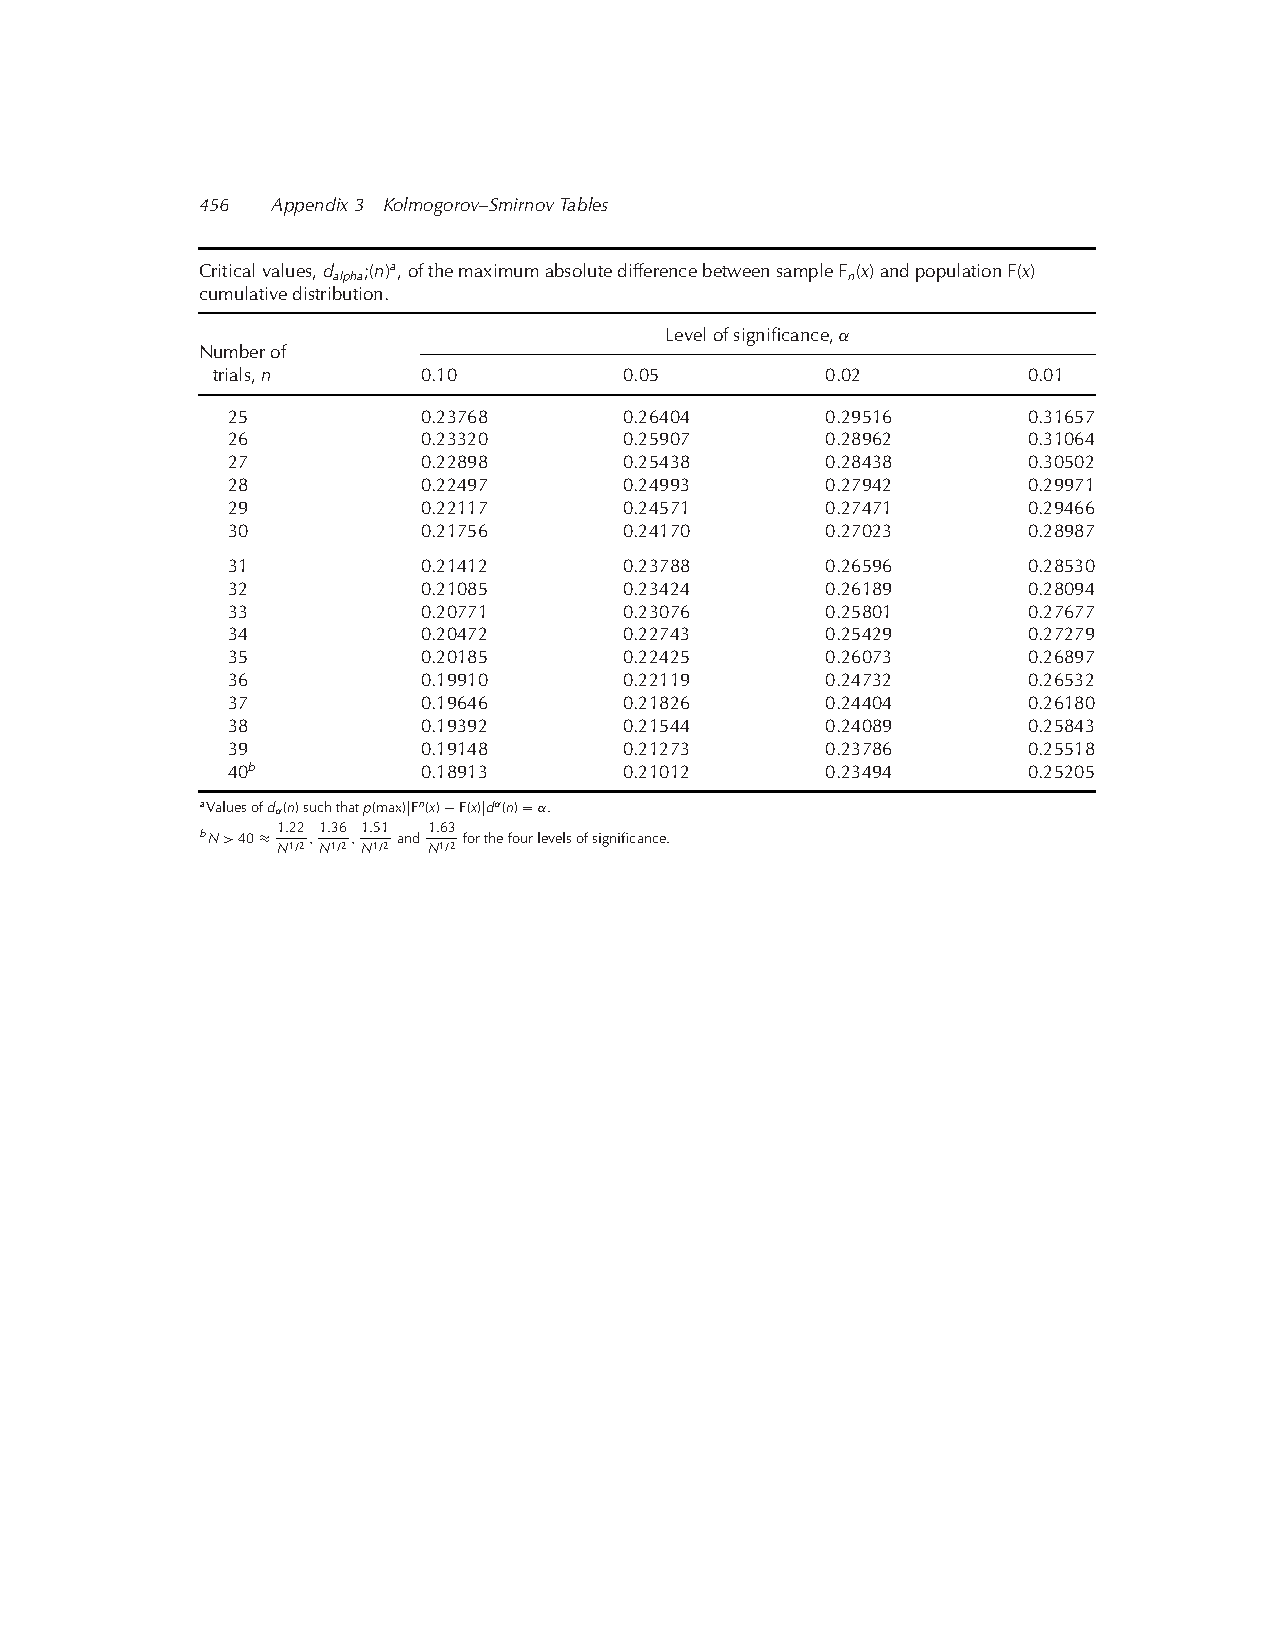
\includepdf{TABLE_KOLMOGOROV_SMIRNOV_2.pdf}

\newpage

\section{\texorpdfstring{\textcolor{blue}{Chapitre 4 : Problème de k > 2 échantillons}}{}}\label{section-3}

\subsection{Test de Kruskal - Wallis}\label{test-de-kruskal---wallis}

\begin{Shaded}
\begin{Highlighting}[]
\CommentTok{\# Données}
\NormalTok{salaire }\OtherTok{\textless{}{-}} \FunctionTok{c}\NormalTok{(}\DecValTok{420}\NormalTok{, }\DecValTok{450}\NormalTok{, }\DecValTok{470}\NormalTok{, }\DecValTok{490}\NormalTok{,   }\CommentTok{\# X1 : économie}
             \DecValTok{410}\NormalTok{, }\DecValTok{430}\NormalTok{, }\DecValTok{440}\NormalTok{, }\DecValTok{470}\NormalTok{,   }\CommentTok{\# X2 : éducation}
             \DecValTok{400}\NormalTok{, }\DecValTok{410}\NormalTok{, }\DecValTok{430}\NormalTok{, }\DecValTok{440}\NormalTok{)   }\CommentTok{\# X3 : santé}

\NormalTok{ministere }\OtherTok{\textless{}{-}} \FunctionTok{factor}\NormalTok{(}\FunctionTok{rep}\NormalTok{(}\FunctionTok{c}\NormalTok{(}\StringTok{"Economie"}\NormalTok{, }\StringTok{"Education"}\NormalTok{, }\StringTok{"Sante"}\NormalTok{), }\AttributeTok{each =} \DecValTok{4}\NormalTok{))}

\FunctionTok{data.frame}\NormalTok{(salaire, ministere)}
\end{Highlighting}
\end{Shaded}

\begin{verbatim}
##    salaire ministere
## 1      420  Economie
## 2      450  Economie
## 3      470  Economie
## 4      490  Economie
## 5      410 Education
## 6      430 Education
## 7      440 Education
## 8      470 Education
## 9      400     Sante
## 10     410     Sante
## 11     430     Sante
## 12     440     Sante
\end{verbatim}

On veut tester :

\(H_0\) : le salaire a les mêmes distributions contre \(H_1\) : au moins
une distribution est différente

\subsubsection{Programmation du test de Kruskal -
Wallis}\label{programmation-du-test-de-kruskal---wallis}

\begin{Shaded}
\begin{Highlighting}[]
\CommentTok{\# Calcul des rangs}
\NormalTok{rangs }\OtherTok{\textless{}{-}} \FunctionTok{rank}\NormalTok{(salaire) }
\NormalTok{rangs}
\end{Highlighting}
\end{Shaded}

\begin{verbatim}
##  [1]  4.0  9.0 10.5 12.0  2.5  5.5  7.5 10.5  1.0  2.5  5.5  7.5
\end{verbatim}

\begin{Shaded}
\begin{Highlighting}[]
\CommentTok{\#somme des rangs par groupe}
\NormalTok{data }\OtherTok{\textless{}{-}} \FunctionTok{data.frame}\NormalTok{(salaire, ministere, rangs)}
\NormalTok{S\_i }\OtherTok{\textless{}{-}} \FunctionTok{tapply}\NormalTok{(data}\SpecialCharTok{$}\NormalTok{rangs, data}\SpecialCharTok{$}\NormalTok{ministere, sum)}
\CommentTok{\# Effectifs par groupe}
\NormalTok{n\_i }\OtherTok{\textless{}{-}} \FunctionTok{tapply}\NormalTok{(data}\SpecialCharTok{$}\NormalTok{salaire, data}\SpecialCharTok{$}\NormalTok{ministere, length)}

\FunctionTok{print}\NormalTok{ (S\_i)}
\end{Highlighting}
\end{Shaded}

\begin{verbatim}
##  Economie Education     Sante 
##      35.5      26.0      16.5
\end{verbatim}

\[ H = \dfrac{12}{n (n+1)} \sum_{i = 1}^{K} \dfrac{S_i^2}{n_i} - 3 (n+1) \]

\begin{Shaded}
\begin{Highlighting}[]
\CommentTok{\# Calcul de la statistique H }

\NormalTok{n }\OtherTok{\textless{}{-}} \FunctionTok{length}\NormalTok{(salaire)}
\NormalTok{H }\OtherTok{\textless{}{-}}\NormalTok{ (}\DecValTok{12} \SpecialCharTok{/}\NormalTok{ (n }\SpecialCharTok{*}\NormalTok{ (n}\SpecialCharTok{+} \DecValTok{1}\NormalTok{))) }\SpecialCharTok{*} \FunctionTok{sum}\NormalTok{((S\_i}\SpecialCharTok{\^{}}\DecValTok{2}\NormalTok{) }\SpecialCharTok{/}\NormalTok{ n\_i) }\SpecialCharTok{{-}} \DecValTok{3} \SpecialCharTok{*}\NormalTok{ (n}\SpecialCharTok{+} \DecValTok{1}\NormalTok{)}
\FunctionTok{print}\NormalTok{(H)}
\end{Highlighting}
\end{Shaded}

\begin{verbatim}
## [1] 3.471154
\end{verbatim}

Sous H0, H suit une loi de Khi-deux à 3-1 degrés de liberté.

\begin{Shaded}
\begin{Highlighting}[]
\CommentTok{\# nombre de degrés de libertés}
\NormalTok{ddl }\OtherTok{\textless{}{-}} \FunctionTok{length}\NormalTok{(}\FunctionTok{unique}\NormalTok{(ministere)) }\SpecialCharTok{{-}} \DecValTok{1}  
\CommentTok{\# valeur critique de la table de la loi de Khi{-}deux }
\NormalTok{stat\_theo }\OtherTok{\textless{}{-}} \FunctionTok{qchisq}\NormalTok{(}\FloatTok{0.95}\NormalTok{, }\AttributeTok{df =} \DecValTok{2}\NormalTok{)}
\NormalTok{p\_value }\OtherTok{\textless{}{-}} \DecValTok{1} \SpecialCharTok{{-}} \FunctionTok{pchisq}\NormalTok{(H, ddl)}

\FunctionTok{cat}\NormalTok{(}\StringTok{"Statistique calculée ="}\NormalTok{, }\FunctionTok{round}\NormalTok{(H, }\DecValTok{3}\NormalTok{), }\StringTok{"}\SpecialCharTok{\textbackslash{}n}\StringTok{"}\NormalTok{)}
\end{Highlighting}
\end{Shaded}

\begin{verbatim}
## Statistique calculée = 3.471
\end{verbatim}

\begin{Shaded}
\begin{Highlighting}[]
\FunctionTok{cat}\NormalTok{(}\StringTok{"valeur critique ="}\NormalTok{, }\FunctionTok{round}\NormalTok{(stat\_theo, }\DecValTok{3}\NormalTok{), }\StringTok{"}\SpecialCharTok{\textbackslash{}n}\StringTok{"}\NormalTok{)}
\end{Highlighting}
\end{Shaded}

\begin{verbatim}
## valeur critique = 5.991
\end{verbatim}

\begin{Shaded}
\begin{Highlighting}[]
\FunctionTok{cat}\NormalTok{(}\StringTok{"p{-}value ="}\NormalTok{, }\FunctionTok{round}\NormalTok{(p\_value,}\DecValTok{3}\NormalTok{), }\StringTok{"}\SpecialCharTok{\textbackslash{}n}\StringTok{"}\NormalTok{)}
\end{Highlighting}
\end{Shaded}

\begin{verbatim}
## p-value = 0.176
\end{verbatim}

3.47 \textless{} 5.99. Ainsi, au seuil de \$ \alpha = \$ 5 \%, on ne
peut rejeter H0. C'est dire que les distributions de salaires sont
identiques.

\subsubsection{Avec Kruskal.test}\label{avec-kruskal.test}

\begin{Shaded}
\begin{Highlighting}[]
\FunctionTok{kruskal.test}\NormalTok{(salaire }\SpecialCharTok{\textasciitilde{}}\NormalTok{ ministere)}
\end{Highlighting}
\end{Shaded}

\begin{verbatim}
## 
##  Kruskal-Wallis rank sum test
## 
## data:  salaire by ministere
## Kruskal-Wallis chi-squared = 3.5204, df = 2, p-value = 0.172
\end{verbatim}

p-value \textgreater{} 0.05. Ainsi, au seuil de \(\alpha =\) 5 \%, on ne
peut rejeter H0. C'est dire que les distributions de salaires sont
identiques.

\subsubsection{Correction des ex-aequos}\label{correction-des-ex-aequos}

Les rangs moyens utilisés dans le test introduisent une distorsion dans
la distribution de H si des ex-aequos existent.

\[ H_{corrigé} = \dfrac{H}{1- \sum_{i=1}^s \dfrac{(t_i^3 - t_i)}{n^3 - n}} \]

\begin{Shaded}
\begin{Highlighting}[]
\CommentTok{\# Identification des tailles des groupes d\textquotesingle{}ex{-}aequos}
\NormalTok{freq }\OtherTok{\textless{}{-}} \FunctionTok{table}\NormalTok{(salaire)          }\CommentTok{\# compte les fréquences des valeurs}
\NormalTok{ties }\OtherTok{\textless{}{-}}\NormalTok{ freq[freq }\SpecialCharTok{\textgreater{}} \DecValTok{1}\NormalTok{]          }\CommentTok{\# garde seulement celles \textgreater{} 1}
\NormalTok{sum\_ties }\OtherTok{\textless{}{-}} \FunctionTok{sum}\NormalTok{(ties}\SpecialCharTok{\^{}}\DecValTok{3} \SpecialCharTok{{-}}\NormalTok{ ties)  }\CommentTok{\# somme des (t\_i\^{}3 {-} t\_i)}

\CommentTok{\# Correction}
\NormalTok{correction }\OtherTok{\textless{}{-}} \DecValTok{1} \SpecialCharTok{{-}}\NormalTok{ (sum\_ties }\SpecialCharTok{/}\NormalTok{ (n}\SpecialCharTok{\^{}}\DecValTok{3} \SpecialCharTok{{-}}\NormalTok{ n))}
\NormalTok{H\_corrige }\OtherTok{\textless{}{-}}\NormalTok{ H }\SpecialCharTok{/}\NormalTok{ correction}

\CommentTok{\# 3. Affichage}
\FunctionTok{cat}\NormalTok{(}\StringTok{"H ="}\NormalTok{, }\FunctionTok{round}\NormalTok{(H,}\DecValTok{3}\NormalTok{), }\StringTok{"}\SpecialCharTok{\textbackslash{}n}\StringTok{"}\NormalTok{)}
\end{Highlighting}
\end{Shaded}

\begin{verbatim}
## H = 3.471
\end{verbatim}

\begin{Shaded}
\begin{Highlighting}[]
\FunctionTok{cat}\NormalTok{(}\StringTok{"Facteur de correction ="}\NormalTok{, }\FunctionTok{round}\NormalTok{(correction,}\DecValTok{3}\NormalTok{), }\StringTok{"}\SpecialCharTok{\textbackslash{}n}\StringTok{"}\NormalTok{)}
\end{Highlighting}
\end{Shaded}

\begin{verbatim}
## Facteur de correction = 0.986
\end{verbatim}

\begin{Shaded}
\begin{Highlighting}[]
\FunctionTok{cat}\NormalTok{(}\StringTok{"H corrigée ="}\NormalTok{, }\FunctionTok{round}\NormalTok{(H\_corrige,}\DecValTok{3}\NormalTok{), }\StringTok{"}\SpecialCharTok{\textbackslash{}n}\StringTok{"}\NormalTok{)}
\end{Highlighting}
\end{Shaded}

\begin{verbatim}
## H corrigée = 3.52
\end{verbatim}

\begin{Shaded}
\begin{Highlighting}[]
\FunctionTok{cat}\NormalTok{(}\StringTok{"Valeur critique ="}\NormalTok{, }\FunctionTok{round}\NormalTok{(}\FunctionTok{qchisq}\NormalTok{(}\FloatTok{0.95}\NormalTok{, }\DecValTok{2}\NormalTok{),}\DecValTok{3}\NormalTok{), }\StringTok{"}\SpecialCharTok{\textbackslash{}n}\StringTok{"}\NormalTok{)}
\end{Highlighting}
\end{Shaded}

\begin{verbatim}
## Valeur critique = 5.991
\end{verbatim}

3.52 \textless{} 5.991 donc on ne peut rejeter H0.

\textbf{NB :} La fonction \textbf{Kruskal.test} corrige les ex-aequos.

\newpage

\section{\texorpdfstring{\textcolor{blue}{CHAPITRE 5 : Estimation d'une densité }}{}}\label{section-4}

\subsection{Estimation de la densité par
histogramme}\label{estimation-de-la-densituxe9-par-histogramme}

\subsubsection{Construction de l'estimateur par
l'histogramme}\label{construction-de-lestimateur-par-lhistogramme}

Soit \([a;b]\) l'intervalle contenant les observations
\(x_1, x_2, \ldots, x_n\).

On partitionne l'intervalle \([a;b]\) en \(J\) classes de longueur
\(h\). Les classes sont notées par :

\[
A_j = [a_j; a_{j+1}], \quad j = 1, 2, \ldots, J
\]

avec

\[
h = a_{j+1} - a_j
\]

Si on note \(n_j\) le nombre d'observations de l'échantillon appartenant
à la classe \(A_j\), alors :

\[
n_j = \mathrm{card}\{ i : x_i \in A_j \} = \sum_{i=1}^n 1_{\{x_i \in A_j\}}
\]

L'estimateur de la densité \(f\) sur la classe \(A_j\) est donné par :

\[
\hat{f}_n(x) = \frac{n_j}{n \cdot h}, \quad x \in [a_j, a_{j+1}]
\]

On peut aussi écrire :

\[
\hat{f}_n(x) = \frac{1}{n} \cdot \frac{\mathrm{card}\{ x_i \leq a_{j+1} \} - \mathrm{card}\{ x_i \leq a_j \}}{h}
\]

\textbf{Note :} Cet estimateur est une fonction en escalier, constante
sur chaque classe \(A_j\).

\subsubsection{Application}\label{application-2}

\begin{Shaded}
\begin{Highlighting}[]
\CommentTok{\# Données}
\NormalTok{X }\OtherTok{\textless{}{-}} \FunctionTok{c}\NormalTok{(}\FloatTok{1.1}\NormalTok{, }\FloatTok{2.3}\NormalTok{, }\FloatTok{1.7}\NormalTok{, }\FloatTok{2.8}\NormalTok{, }\FloatTok{3.2}\NormalTok{, }\FloatTok{1.9}\NormalTok{, }\FloatTok{2.5}\NormalTok{, }\FloatTok{3.7}\NormalTok{, }\FloatTok{2.9}\NormalTok{, }\FloatTok{2.1}\NormalTok{)}

\CommentTok{\# Taille de l\textquotesingle{}échantillon}
\NormalTok{n }\OtherTok{\textless{}{-}} \FunctionTok{length}\NormalTok{(X)}

\CommentTok{\# Définition des bornes de l\textquotesingle{}intervalle}
\NormalTok{a }\OtherTok{\textless{}{-}} \FunctionTok{min}\NormalTok{(X)}
\NormalTok{b }\OtherTok{\textless{}{-}} \FunctionTok{max}\NormalTok{(X)}

\CommentTok{\# Nombre de classes}
\NormalTok{J }\OtherTok{\textless{}{-}} \DecValTok{4}

\CommentTok{\# Largeur des classes}
\NormalTok{h }\OtherTok{\textless{}{-}}\NormalTok{ (b }\SpecialCharTok{{-}}\NormalTok{ a) }\SpecialCharTok{/}\NormalTok{ J}

\CommentTok{\# Définition des bornes des classes}
\NormalTok{breaks }\OtherTok{\textless{}{-}} \FunctionTok{seq}\NormalTok{(a, b, }\AttributeTok{by =}\NormalTok{ h)}
\end{Highlighting}
\end{Shaded}

\paragraph{Construisons à présent
l'estimateur}\label{construisons-uxe0-pruxe9sent-lestimateur}

\begin{Shaded}
\begin{Highlighting}[]
\CommentTok{\# Construction de l’histogramme }
\NormalTok{hist\_res }\OtherTok{\textless{}{-}} \FunctionTok{hist}\NormalTok{(X, }\AttributeTok{breaks =}\NormalTok{ breaks, }\AttributeTok{plot =} \ConstantTok{FALSE}\NormalTok{)}

\CommentTok{\# Effectifs par classe (n\_j)}
\NormalTok{n\_j }\OtherTok{\textless{}{-}}\NormalTok{ hist\_res}\SpecialCharTok{$}\NormalTok{counts}

\CommentTok{\# Estimateur de la densité par classe}
\NormalTok{f\_hat }\OtherTok{\textless{}{-}}\NormalTok{ n\_j }\SpecialCharTok{/}\NormalTok{ (n }\SpecialCharTok{*}\NormalTok{ h)}

\CommentTok{\# Affichage des résultats}
\FunctionTok{data.frame}\NormalTok{(}
  \AttributeTok{Classe =} \FunctionTok{paste0}\NormalTok{(}\StringTok{"["}\NormalTok{, }\FunctionTok{round}\NormalTok{(breaks[}\SpecialCharTok{{-}}\FunctionTok{length}\NormalTok{(breaks)], }\DecValTok{2}\NormalTok{), }\StringTok{", "}\NormalTok{, }\FunctionTok{round}\NormalTok{(breaks[}\SpecialCharTok{{-}}\DecValTok{1}\NormalTok{], }\DecValTok{2}\NormalTok{), }\StringTok{"]"}\NormalTok{),}
  \AttributeTok{Effectif =}\NormalTok{ n\_j,}
  \AttributeTok{Densite\_estimee =} \FunctionTok{round}\NormalTok{(f\_hat, }\DecValTok{3}\NormalTok{)}
\NormalTok{)}
\end{Highlighting}
\end{Shaded}

\begin{verbatim}
##        Classe Effectif Densite_estimee
## 1 [1.1, 1.75]        2           0.308
## 2 [1.75, 2.4]        3           0.462
## 3 [2.4, 3.05]        3           0.462
## 4 [3.05, 3.7]        2           0.308
\end{verbatim}

\textbf{Traçons l'histogramme}

\begin{Shaded}
\begin{Highlighting}[]
\CommentTok{\# Tracé de l’histogramme}
\NormalTok{hist\_res }\OtherTok{\textless{}{-}} \FunctionTok{hist}\NormalTok{(X, }\AttributeTok{breaks =}\NormalTok{ breaks, }\AttributeTok{freq =} \ConstantTok{FALSE}\NormalTok{, }\AttributeTok{col =} \StringTok{"skyblue"}\NormalTok{,}
                 \AttributeTok{main =} \StringTok{"Estimateur par histogramme"}\NormalTok{,}
                 \AttributeTok{xlab =} \StringTok{"X"}\NormalTok{, }\AttributeTok{ylab =} \StringTok{"Densité estimée"}\NormalTok{, }\AttributeTok{border =} \StringTok{"darkblue"}\NormalTok{)}

\CommentTok{\# Coordonnées du polygone des fréquences :}
\CommentTok{\# abscisses = milieux des classes}
\NormalTok{mids }\OtherTok{\textless{}{-}}\NormalTok{ hist\_res}\SpecialCharTok{$}\NormalTok{mids}

\CommentTok{\# ordonnées = densité estimée (f\_hat)}
\NormalTok{densites }\OtherTok{\textless{}{-}}\NormalTok{ hist\_res}\SpecialCharTok{$}\NormalTok{density}

\CommentTok{\# Tracé de la ligne du polygone des fréquences}
\FunctionTok{lines}\NormalTok{(mids, densites, }\AttributeTok{type =} \StringTok{"b"}\NormalTok{, }\AttributeTok{col =} \StringTok{"red"}\NormalTok{, }\AttributeTok{lwd =} \DecValTok{2}\NormalTok{, }\AttributeTok{pch =} \DecValTok{19}\NormalTok{)}
\end{Highlighting}
\end{Shaded}

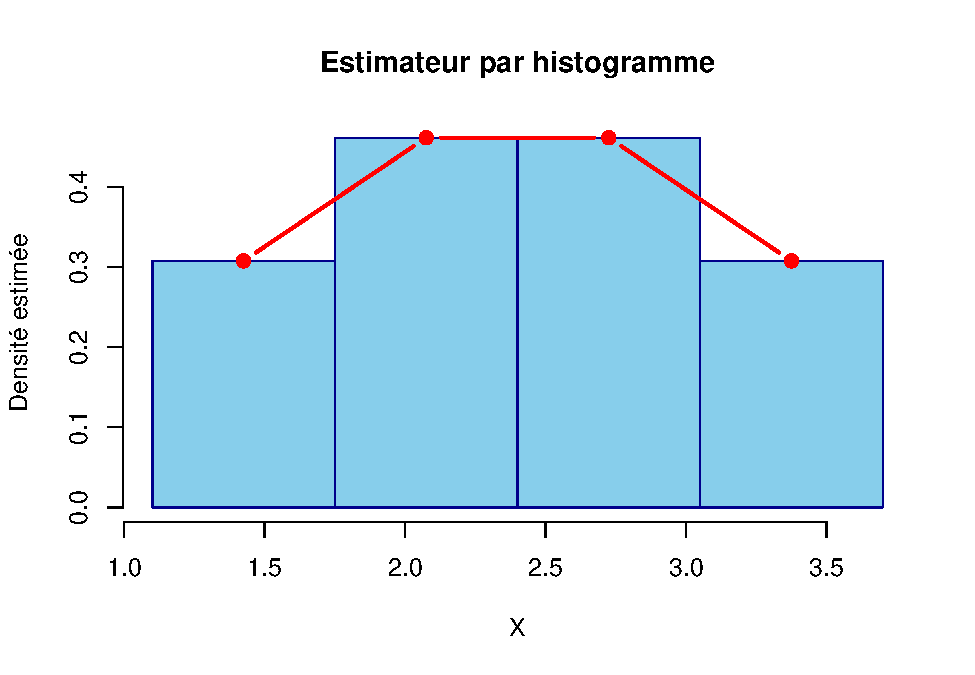
\includegraphics{Stat_non_para_files/figure-latex/unnamed-chunk-134-1.pdf}

\subsubsection{Estimation de la MISE et calcul de
l'AMISE}\label{estimation-de-la-mise-et-calcul-de-lamise}

\begin{itemize}
\tightlist
\item
  \textbf{Définition de l'erreur quadratique moyenne intégrée (MISE)}
\end{itemize}

L'erreur quadratique moyenne intégrée (MISE) est définie par :

\[
\text{MISE} = \int_{-\infty}^{+\infty} E\left[(\hat{f}_n(x) - f(x))^2\right] dx
\]

Pour l'estimateur par histogramme, l'approximation asymptotique de la
MISE est :

\[
\text{MISE} \approx \frac{h^2}{12}\int_{-\infty}^{+\infty} (f'(x))^2 dx + \frac{1}{nh} + o(h^2) + o\left(\frac{1}{nh}\right)
\]

Le terme principal du MISE, appelé AMISE (MISE asymptotique), est :

\[
\text{AMISE} = \frac{h^2}{12}\int_{-\infty}^{+\infty} (f'(x))^2 dx + \frac{1}{nh}
\]

\begin{Shaded}
\begin{Highlighting}[]
\CommentTok{\# Données }
\NormalTok{X }\OtherTok{\textless{}{-}} \FunctionTok{c}\NormalTok{(}\FloatTok{1.1}\NormalTok{, }\FloatTok{2.3}\NormalTok{, }\FloatTok{1.7}\NormalTok{, }\FloatTok{2.8}\NormalTok{, }\FloatTok{3.2}\NormalTok{, }\FloatTok{1.9}\NormalTok{, }\FloatTok{2.5}\NormalTok{, }\FloatTok{3.7}\NormalTok{, }\FloatTok{2.9}\NormalTok{, }\FloatTok{2.1}\NormalTok{)}
\NormalTok{n }\OtherTok{\textless{}{-}} \FunctionTok{length}\NormalTok{(X)}
\NormalTok{mu }\OtherTok{\textless{}{-}} \FunctionTok{mean}\NormalTok{(X)}
\NormalTok{sigma }\OtherTok{\textless{}{-}} \FunctionTok{sd}\NormalTok{(X)}

\CommentTok{\# Paramètres de l\textquotesingle{}histogramme}
\NormalTok{J }\OtherTok{\textless{}{-}} \DecValTok{4}
\NormalTok{h }\OtherTok{\textless{}{-}}\NormalTok{ (}\FunctionTok{max}\NormalTok{(X) }\SpecialCharTok{{-}} \FunctionTok{min}\NormalTok{(X)) }\SpecialCharTok{/}\NormalTok{ J}
\end{Highlighting}
\end{Shaded}

\begin{itemize}
\tightlist
\item
  \textbf{Estimation empirique du MISE par simulation Monte Carlo}
\end{itemize}

Pour estimer empiriquement le MISE, on utilise la simulation Monte Carlo
avec la formule :

\[
\text{MISE} \approx \frac{1}{B} \sum_{b=1}^{B} \int (\hat{f}_n^{(b)}(x) - f(x))^2 dx
\]

où \(\hat{f}_n^{(b)}(x)\) est l'estimateur calculé sur le \(b\)-ième
échantillon simulé et \(B\) est le nombre de répétitions Monte Carlo.

\begin{itemize}
\tightlist
\item
  \textbf{Estimation de la MISE et calcul de l'AMISE}
\end{itemize}

\begin{Shaded}
\begin{Highlighting}[]
\CommentTok{\# Données }
\NormalTok{X }\OtherTok{\textless{}{-}} \FunctionTok{c}\NormalTok{(}\FloatTok{1.1}\NormalTok{, }\FloatTok{2.3}\NormalTok{, }\FloatTok{1.7}\NormalTok{, }\FloatTok{2.8}\NormalTok{, }\FloatTok{3.2}\NormalTok{, }\FloatTok{1.9}\NormalTok{, }\FloatTok{2.5}\NormalTok{, }\FloatTok{3.7}\NormalTok{, }\FloatTok{2.9}\NormalTok{, }\FloatTok{2.1}\NormalTok{)}
\NormalTok{n }\OtherTok{\textless{}{-}} \FunctionTok{length}\NormalTok{(X)}
\NormalTok{mu }\OtherTok{\textless{}{-}} \FunctionTok{mean}\NormalTok{(X)}
\NormalTok{sigma }\OtherTok{\textless{}{-}} \FunctionTok{sd}\NormalTok{(X)}

\CommentTok{\# Paramètres de l’histogramme}
\NormalTok{J }\OtherTok{\textless{}{-}} \DecValTok{4}
\NormalTok{h }\OtherTok{\textless{}{-}}\NormalTok{ (}\FunctionTok{max}\NormalTok{(X) }\SpecialCharTok{{-}} \FunctionTok{min}\NormalTok{(X)) }\SpecialCharTok{/}\NormalTok{ J}
\end{Highlighting}
\end{Shaded}

\begin{Shaded}
\begin{Highlighting}[]
\CommentTok{\# Estimation empirique du MISE par simulation}
\NormalTok{B }\OtherTok{\textless{}{-}} \DecValTok{500}  \CommentTok{\# nombre de répétitions Monte Carlo}
\NormalTok{grid\_x }\OtherTok{\textless{}{-}} \FunctionTok{seq}\NormalTok{(}\FunctionTok{min}\NormalTok{(X)}\SpecialCharTok{{-}}\DecValTok{1}\NormalTok{, }\FunctionTok{max}\NormalTok{(X)}\SpecialCharTok{+}\DecValTok{1}\NormalTok{, }\AttributeTok{length.out =} \DecValTok{500}\NormalTok{)}
\NormalTok{true\_density }\OtherTok{\textless{}{-}} \FunctionTok{dnorm}\NormalTok{(grid\_x, }\AttributeTok{mean =}\NormalTok{ mu, }\AttributeTok{sd =}\NormalTok{ sigma)}
\NormalTok{mise\_vals }\OtherTok{\textless{}{-}} \FunctionTok{numeric}\NormalTok{(B)}

\ControlFlowTok{for}\NormalTok{ (b }\ControlFlowTok{in} \DecValTok{1}\SpecialCharTok{:}\NormalTok{B) \{}
  \CommentTok{\# Génération d\textquotesingle{}un nouvel échantillon}
\NormalTok{  sample\_b }\OtherTok{\textless{}{-}} \FunctionTok{rnorm}\NormalTok{(n, }\AttributeTok{mean =}\NormalTok{ mu, }\AttributeTok{sd =}\NormalTok{ sigma)}
\NormalTok{  breaks\_b }\OtherTok{\textless{}{-}} \FunctionTok{seq}\NormalTok{(}\FunctionTok{min}\NormalTok{(sample\_b), }\FunctionTok{max}\NormalTok{(sample\_b), }\AttributeTok{length.out =}\NormalTok{ J }\SpecialCharTok{+} \DecValTok{1}\NormalTok{)}
\NormalTok{  hist\_b }\OtherTok{\textless{}{-}} \FunctionTok{hist}\NormalTok{(sample\_b, }\AttributeTok{breaks =}\NormalTok{ breaks\_b, }\AttributeTok{plot =} \ConstantTok{FALSE}\NormalTok{)}
\NormalTok{  mids\_b }\OtherTok{\textless{}{-}}\NormalTok{ hist\_b}\SpecialCharTok{$}\NormalTok{mids}
\NormalTok{  f\_hat\_b }\OtherTok{\textless{}{-}}\NormalTok{ hist\_b}\SpecialCharTok{$}\NormalTok{density}
  
  \CommentTok{\# Interpolation de la densité estimée}
\NormalTok{  f\_interp }\OtherTok{\textless{}{-}} \FunctionTok{approx}\NormalTok{(}\AttributeTok{x =}\NormalTok{ mids\_b, }\AttributeTok{y =}\NormalTok{ f\_hat\_b, }\AttributeTok{xout =}\NormalTok{ grid\_x,}
                     \AttributeTok{method =} \StringTok{"constant"}\NormalTok{, }\AttributeTok{rule =} \DecValTok{2}\NormalTok{)}\SpecialCharTok{$}\NormalTok{y}
  
  \CommentTok{\# Calcul de l’erreur quadratique intégrée}
\NormalTok{  mise\_vals[b] }\OtherTok{\textless{}{-}} \FunctionTok{mean}\NormalTok{((f\_interp }\SpecialCharTok{{-}}\NormalTok{ true\_density)}\SpecialCharTok{\^{}}\DecValTok{2}\NormalTok{)}
\NormalTok{\}}

\CommentTok{\# Moyenne des erreurs → estimation du MISE}
\NormalTok{MISE\_estimee }\OtherTok{\textless{}{-}} \FunctionTok{mean}\NormalTok{(mise\_vals)}

\CommentTok{\# Calcul théorique de l’AMISE}
\CommentTok{\# Pour la densité normale N(mu, sigma\^{}2), on connaît :}
\NormalTok{I\_fprime2 }\OtherTok{\textless{}{-}} \DecValTok{1} \SpecialCharTok{/}\NormalTok{ (}\DecValTok{2} \SpecialCharTok{*}\NormalTok{ pi }\SpecialCharTok{*}\NormalTok{ sigma}\SpecialCharTok{\^{}}\DecValTok{5}\NormalTok{)  }\CommentTok{\# ∫ (f\textquotesingle{})\^{}2 dx}
\NormalTok{AMISE }\OtherTok{\textless{}{-}}\NormalTok{ (}\DecValTok{1} \SpecialCharTok{/}\NormalTok{ (n }\SpecialCharTok{*}\NormalTok{ h)) }\SpecialCharTok{+}\NormalTok{ (h}\SpecialCharTok{\^{}}\DecValTok{2} \SpecialCharTok{/} \DecValTok{12}\NormalTok{) }\SpecialCharTok{*}\NormalTok{ I\_fprime2}

\CommentTok{\# Affichage des résultats}
\FunctionTok{cat}\NormalTok{(}\StringTok{"Estimation empirique du MISE :"}\NormalTok{, }\FunctionTok{round}\NormalTok{(MISE\_estimee, }\DecValTok{6}\NormalTok{), }\StringTok{"}\SpecialCharTok{\textbackslash{}n}\StringTok{"}\NormalTok{)}
\end{Highlighting}
\end{Shaded}

\begin{verbatim}
## Estimation empirique du MISE : 0.180887
\end{verbatim}

\begin{Shaded}
\begin{Highlighting}[]
\FunctionTok{cat}\NormalTok{(}\StringTok{"Valeur théorique de l’AMISE   :"}\NormalTok{, }\FunctionTok{round}\NormalTok{(AMISE, }\DecValTok{6}\NormalTok{), }\StringTok{"}\SpecialCharTok{\textbackslash{}n}\StringTok{"}\NormalTok{)}
\end{Highlighting}
\end{Shaded}

\begin{verbatim}
## Valeur théorique de l’AMISE   : 0.175143
\end{verbatim}

\paragraph{Calcul théorique de
l'AMISE}\label{calcul-thuxe9orique-de-lamise}

Pour une densité normale \(N(\mu, \sigma^2)\), on connaît la valeur
analytique de :

\[
\int_{-\infty}^{+\infty} (f'(x))^2 dx = \frac{1}{2\pi^{1/2}\sigma^5}
\]

D'où l'AMISE théorique pour la densité normale :

\[
\text{AMISE} = \frac{h^2}{12} \times \frac{1}{2\pi^{1/2}\sigma^5} + \frac{1}{nh}
\]

\begin{Shaded}
\begin{Highlighting}[]
\CommentTok{\# Calcul théorique de l\textquotesingle{}AMISE}
\CommentTok{\# Pour la densité normale N(mu, sigma²), on connaît :}
\NormalTok{I\_fprime2 }\OtherTok{\textless{}{-}} \DecValTok{1} \SpecialCharTok{/}\NormalTok{ (}\DecValTok{2} \SpecialCharTok{*}\NormalTok{ pi }\SpecialCharTok{*}\NormalTok{ sigma}\SpecialCharTok{\^{}}\DecValTok{5}\NormalTok{)  }\CommentTok{\# }
\NormalTok{AMISE }\OtherTok{\textless{}{-}}\NormalTok{ (}\DecValTok{1} \SpecialCharTok{/}\NormalTok{ (n }\SpecialCharTok{*}\NormalTok{ h)) }\SpecialCharTok{+}\NormalTok{ (h}\SpecialCharTok{\^{}}\DecValTok{2} \SpecialCharTok{/} \DecValTok{12}\NormalTok{) }\SpecialCharTok{*}\NormalTok{ I\_fprime2}

\CommentTok{\# Affichage des résultats}
\FunctionTok{cat}\NormalTok{(}\StringTok{"Estimation empirique du MISE :"}\NormalTok{, }\FunctionTok{round}\NormalTok{(MISE\_estimee, }\DecValTok{6}\NormalTok{), }\StringTok{"}\SpecialCharTok{\textbackslash{}n}\StringTok{"}\NormalTok{)}
\end{Highlighting}
\end{Shaded}

\begin{verbatim}
## Estimation empirique du MISE : 0.180887
\end{verbatim}

\begin{Shaded}
\begin{Highlighting}[]
\FunctionTok{cat}\NormalTok{(}\StringTok{"Valeur théorique de l\textquotesingle{}AMISE   :"}\NormalTok{, }\FunctionTok{round}\NormalTok{(AMISE, }\DecValTok{6}\NormalTok{), }\StringTok{"}\SpecialCharTok{\textbackslash{}n}\StringTok{"}\NormalTok{)}
\end{Highlighting}
\end{Shaded}

\begin{verbatim}
## Valeur théorique de l'AMISE   : 0.175143
\end{verbatim}

\subsubsection{\texorpdfstring{Calcul de la fenêtre optimale
\(h^*\)}{Calcul de la fenêtre optimale h\^{}*}}\label{calcul-de-la-fenuxeatre-optimale-h}

La fenêtre optimale théorique qui minimise l'AMISE est obtenue en
résolvant :

\[
\frac{d}{dh}(\text{AMISE}) = 0
\]

Ce qui donne :

\[
h^* = \left[\frac{6}{n \times \int_{-\infty}^{+\infty} (f'(x))^2 dx}\right]^{1/3}
\]

L'AMISE avec la fenêtre optimale est proportionnelle à \(n^{-2/3}\), ce
qui donne la vitesse de convergence de l'estimateur par histogramme.

\begin{Shaded}
\begin{Highlighting}[]
\CommentTok{\# Calcul de la fenêtre optimale}
\NormalTok{h\_optimal }\OtherTok{\textless{}{-}}\NormalTok{ (}\DecValTok{6} \SpecialCharTok{/}\NormalTok{ (n }\SpecialCharTok{*}\NormalTok{ I\_fprime2))}\SpecialCharTok{\^{}}\NormalTok{(}\DecValTok{1}\SpecialCharTok{/}\DecValTok{3}\NormalTok{)}

\CommentTok{\# AMISE avec la fenêtre optimale}
\NormalTok{AMISE\_optimal }\OtherTok{\textless{}{-}}\NormalTok{ (h\_optimal}\SpecialCharTok{\^{}}\DecValTok{2} \SpecialCharTok{/} \DecValTok{12}\NormalTok{) }\SpecialCharTok{*}\NormalTok{ I\_fprime2 }\SpecialCharTok{+} \DecValTok{1} \SpecialCharTok{/}\NormalTok{ (n }\SpecialCharTok{*}\NormalTok{ h\_optimal)}

\FunctionTok{cat}\NormalTok{(}\StringTok{"Fenêtre optimale h*           :"}\NormalTok{, }\FunctionTok{round}\NormalTok{(h\_optimal, }\DecValTok{4}\NormalTok{), }\StringTok{"}\SpecialCharTok{\textbackslash{}n}\StringTok{"}\NormalTok{)}
\end{Highlighting}
\end{Shaded}

\begin{verbatim}
## Fenêtre optimale h*           : 0.9973
\end{verbatim}

\begin{Shaded}
\begin{Highlighting}[]
\FunctionTok{cat}\NormalTok{(}\StringTok{"AMISE avec h* optimal         :"}\NormalTok{, }\FunctionTok{round}\NormalTok{(AMISE\_optimal, }\DecValTok{6}\NormalTok{), }\StringTok{"}\SpecialCharTok{\textbackslash{}n}\StringTok{"}\NormalTok{)}
\end{Highlighting}
\end{Shaded}

\begin{verbatim}
## AMISE avec h* optimal         : 0.150405
\end{verbatim}

\begin{Shaded}
\begin{Highlighting}[]
\FunctionTok{cat}\NormalTok{(}\StringTok{"Fenêtre utilisée h            :"}\NormalTok{, }\FunctionTok{round}\NormalTok{(h, }\DecValTok{4}\NormalTok{), }\StringTok{"}\SpecialCharTok{\textbackslash{}n}\StringTok{"}\NormalTok{)}
\end{Highlighting}
\end{Shaded}

\begin{verbatim}
## Fenêtre utilisée h            : 0.65
\end{verbatim}

\subsubsection{Calcul de h de façon
automatique}\label{calcul-de-h-de-fauxe7on-automatique}

\begin{Shaded}
\begin{Highlighting}[]
\NormalTok{X }\OtherTok{\textless{}{-}} \FunctionTok{c}\NormalTok{(}\FloatTok{1.1}\NormalTok{, }\FloatTok{2.3}\NormalTok{, }\FloatTok{1.7}\NormalTok{, }\FloatTok{2.8}\NormalTok{, }\FloatTok{3.2}\NormalTok{, }\FloatTok{1.9}\NormalTok{, }\FloatTok{2.5}\NormalTok{, }\FloatTok{3.7}\NormalTok{, }\FloatTok{2.9}\NormalTok{, }\FloatTok{2.1}\NormalTok{)}
\NormalTok{n }\OtherTok{\textless{}{-}} \FunctionTok{length}\NormalTok{(X)}

\CommentTok{\# Choix automatique du nombre de classes selon Sturges}
\NormalTok{J }\OtherTok{\textless{}{-}} \FunctionTok{ceiling}\NormalTok{(}\FunctionTok{log2}\NormalTok{(n) }\SpecialCharTok{+} \DecValTok{1}\NormalTok{)}

\CommentTok{\# Bornes des classes}
\NormalTok{breaks }\OtherTok{\textless{}{-}} \FunctionTok{seq}\NormalTok{(}\FunctionTok{min}\NormalTok{(X), }\FunctionTok{max}\NormalTok{(X), }\AttributeTok{length.out =}\NormalTok{ J }\SpecialCharTok{+} \DecValTok{1}\NormalTok{)}

\CommentTok{\# Histogramme sans affichage}
\NormalTok{hist\_res }\OtherTok{\textless{}{-}} \FunctionTok{hist}\NormalTok{(X, }\AttributeTok{breaks =}\NormalTok{ breaks, }\AttributeTok{plot =} \ConstantTok{FALSE}\NormalTok{)}

\CommentTok{\# Effectifs}
\NormalTok{n\_j }\OtherTok{\textless{}{-}}\NormalTok{ hist\_res}\SpecialCharTok{$}\NormalTok{counts}

\CommentTok{\# Largeur classes (elles sont égales ici)}
\NormalTok{h }\OtherTok{\textless{}{-}} \FunctionTok{diff}\NormalTok{(breaks)[}\DecValTok{1}\NormalTok{]}

\CommentTok{\# Estimation densité}
\NormalTok{f\_hat }\OtherTok{\textless{}{-}}\NormalTok{ n\_j }\SpecialCharTok{/}\NormalTok{ (n }\SpecialCharTok{*}\NormalTok{ h)}

\CommentTok{\# Tableau résultats}
\FunctionTok{data.frame}\NormalTok{(}
  \AttributeTok{Classe =} \FunctionTok{paste0}\NormalTok{(}\StringTok{"["}\NormalTok{, }\FunctionTok{round}\NormalTok{(breaks[}\SpecialCharTok{{-}}\FunctionTok{length}\NormalTok{(breaks)], }\DecValTok{2}\NormalTok{), }\StringTok{", "}\NormalTok{, }\FunctionTok{round}\NormalTok{(breaks[}\SpecialCharTok{{-}}\DecValTok{1}\NormalTok{], }\DecValTok{2}\NormalTok{), }\StringTok{"]"}\NormalTok{),}
  \AttributeTok{Effectif =}\NormalTok{ n\_j,}
  \AttributeTok{Densite\_estimee =} \FunctionTok{round}\NormalTok{(f\_hat, }\DecValTok{3}\NormalTok{)}
\NormalTok{)}
\end{Highlighting}
\end{Shaded}

\begin{verbatim}
##         Classe Effectif Densite_estimee
## 1  [1.1, 1.62]        1           0.192
## 2 [1.62, 2.14]        3           0.577
## 3 [2.14, 2.66]        2           0.385
## 4 [2.66, 3.18]        2           0.385
## 5  [3.18, 3.7]        2           0.385
\end{verbatim}

\begin{Shaded}
\begin{Highlighting}[]
\CommentTok{\# Données}
\NormalTok{X }\OtherTok{\textless{}{-}} \FunctionTok{c}\NormalTok{(}\FloatTok{1.1}\NormalTok{, }\FloatTok{2.3}\NormalTok{, }\FloatTok{1.7}\NormalTok{, }\FloatTok{2.8}\NormalTok{, }\FloatTok{3.2}\NormalTok{, }\FloatTok{1.9}\NormalTok{, }\FloatTok{2.5}\NormalTok{, }\FloatTok{3.7}\NormalTok{, }\FloatTok{2.9}\NormalTok{, }\FloatTok{2.1}\NormalTok{)}

\CommentTok{\# Taille de l\textquotesingle{}échantillon}
\NormalTok{n }\OtherTok{\textless{}{-}} \FunctionTok{length}\NormalTok{(X)}

\CommentTok{\# Définition des bornes de l\textquotesingle{}intervalle}
\NormalTok{a }\OtherTok{\textless{}{-}} \FunctionTok{min}\NormalTok{(X)}
\NormalTok{b }\OtherTok{\textless{}{-}} \FunctionTok{max}\NormalTok{(X)}

\CommentTok{\# Nombre de classes}
\CommentTok{\#J \textless{}{-} 4}

\CommentTok{\# Largeur des classes}
\NormalTok{h }\OtherTok{\textless{}{-}} \FloatTok{0.9973}

\CommentTok{\# Définition des bornes des classes}
\NormalTok{breaks }\OtherTok{\textless{}{-}} \FunctionTok{seq}\NormalTok{(a, b, }\AttributeTok{by =}\NormalTok{ h)}
\end{Highlighting}
\end{Shaded}

\subsubsection{Construisons à présent
l'estimateur}\label{construisons-uxe0-pruxe9sent-lestimateur-1}

\begin{Shaded}
\begin{Highlighting}[]
\CommentTok{\# Construction de l’histogramme }
\NormalTok{hist\_res }\OtherTok{\textless{}{-}} \FunctionTok{hist}\NormalTok{(X, }\AttributeTok{plot =} \ConstantTok{FALSE}\NormalTok{)}

\CommentTok{\# Effectifs par classe (n\_j)}
\NormalTok{n\_j }\OtherTok{\textless{}{-}}\NormalTok{ hist\_res}\SpecialCharTok{$}\NormalTok{counts}

\CommentTok{\# Estimateur de la densité par classe}
\NormalTok{f\_hat }\OtherTok{\textless{}{-}}\NormalTok{ n\_j }\SpecialCharTok{/}\NormalTok{ (n }\SpecialCharTok{*}\NormalTok{ h)}

\CommentTok{\# Affichage des résultats}
\FunctionTok{data.frame}\NormalTok{(}
  \AttributeTok{Classe =} \FunctionTok{paste0}\NormalTok{(}\StringTok{"["}\NormalTok{, }\FunctionTok{round}\NormalTok{(breaks[}\SpecialCharTok{{-}}\FunctionTok{length}\NormalTok{(breaks)], }\DecValTok{2}\NormalTok{), }\StringTok{", "}\NormalTok{, }\FunctionTok{round}\NormalTok{(breaks[}\SpecialCharTok{{-}}\DecValTok{1}\NormalTok{], }\DecValTok{2}\NormalTok{), }\StringTok{"]"}\NormalTok{),}
  \AttributeTok{Effectif =}\NormalTok{ n\_j,}
  \AttributeTok{Densite\_estimee =} \FunctionTok{round}\NormalTok{(f\_hat, }\DecValTok{3}\NormalTok{)}
\NormalTok{)}
\end{Highlighting}
\end{Shaded}

\begin{verbatim}
##        Classe Effectif Densite_estimee
## 1  [1.1, 2.1]        1           0.100
## 2 [2.1, 3.09]        2           0.201
## 3  [1.1, 2.1]        3           0.301
## 4 [2.1, 3.09]        2           0.201
## 5  [1.1, 2.1]        1           0.100
## 6 [2.1, 3.09]        1           0.100
\end{verbatim}

\begin{Shaded}
\begin{Highlighting}[]
\CommentTok{\# Tracé de l’histogramme}
\NormalTok{hist\_res }\OtherTok{\textless{}{-}} \FunctionTok{hist}\NormalTok{(X,  }\AttributeTok{freq =} \ConstantTok{FALSE}\NormalTok{, }\AttributeTok{col =} \StringTok{"skyblue"}\NormalTok{,}
                 \AttributeTok{main =} \StringTok{"Estimateur par histogramme"}\NormalTok{,}
                 \AttributeTok{xlab =} \StringTok{"X"}\NormalTok{, }\AttributeTok{ylab =} \StringTok{"Densité estimée"}\NormalTok{, }\AttributeTok{border =} \StringTok{"darkblue"}\NormalTok{)}

\CommentTok{\# Coordonnées du polygone des fréquences :}
\CommentTok{\# abscisses = milieux des classes}
\NormalTok{mids }\OtherTok{\textless{}{-}}\NormalTok{ hist\_res}\SpecialCharTok{$}\NormalTok{mids}

\CommentTok{\# ordonnées = densité estimée (f\_hat)}
\NormalTok{densites }\OtherTok{\textless{}{-}}\NormalTok{ hist\_res}\SpecialCharTok{$}\NormalTok{density}

\CommentTok{\# Tracé de la ligne du polygone des fréquences}
\FunctionTok{lines}\NormalTok{(mids, densites, }\AttributeTok{type =} \StringTok{"b"}\NormalTok{, }\AttributeTok{col =} \StringTok{"red"}\NormalTok{, }\AttributeTok{lwd =} \DecValTok{2}\NormalTok{, }\AttributeTok{pch =} \DecValTok{19}\NormalTok{)}
\end{Highlighting}
\end{Shaded}

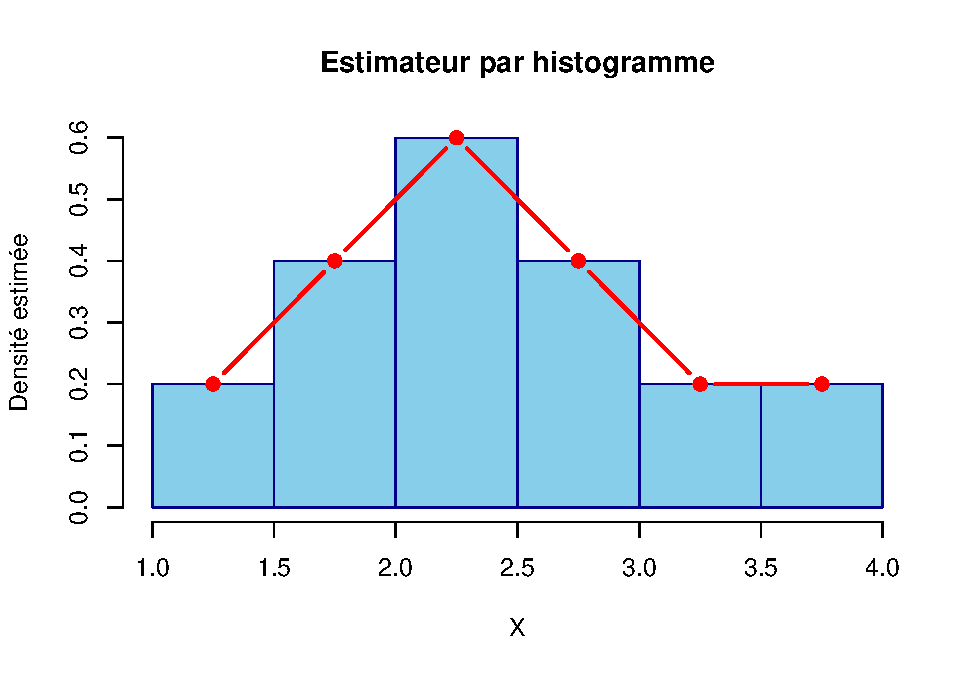
\includegraphics{Stat_non_para_files/figure-latex/unnamed-chunk-143-1.pdf}

\subsection{Estimation par la méthode de l'histogramme : validation
croisée}\label{estimation-par-la-muxe9thode-de-lhistogramme-validation-croisuxe9e}

\subsubsection{Principe de la validation
croisée}\label{principe-de-la-validation-croisuxe9e}

La validation croisée est une méthode générique pour sélectionner des
paramètres de modèles (comme le nombre de classes dans un histogramme)
en évaluant leur performance prédictive. En statistique non
paramétrique, elle permet d'optimiser des estimateurs (densité,
régression, etc.)

\begin{Shaded}
\begin{Highlighting}[]
\FunctionTok{set.seed}\NormalTok{(}\DecValTok{123}\NormalTok{)}
\NormalTok{CV\_hist}\OtherTok{=}\ControlFlowTok{function}\NormalTok{(x) }\CommentTok{\# définition de la fonction en fonction de l\textquotesingle{}échantillon x}
\NormalTok{\{}
\NormalTok{  n}\OtherTok{=}\FunctionTok{length}\NormalTok{(x)}
  \CommentTok{\# valeurs minimale et maximale de x, utilisées pour délimiter les bornes de l’histogramme}
\NormalTok{  a}\OtherTok{=}\FunctionTok{min}\NormalTok{(x)}
\NormalTok{  b}\OtherTok{=}\FunctionTok{max}\NormalTok{(x) }
\NormalTok{  N}\OtherTok{=}\FunctionTok{round}\NormalTok{(n}\SpecialCharTok{/}\DecValTok{5}\NormalTok{); }\CommentTok{\# nombre maximal de classe à tester}
\NormalTok{  b}\OtherTok{=}\NormalTok{b}\SpecialCharTok{+}\NormalTok{(b}\SpecialCharTok{{-}}\NormalTok{a)}\SpecialCharTok{/}\NormalTok{N}
\NormalTok{  m\_CV}\OtherTok{=}\DecValTok{1}
\NormalTok{  J0}\OtherTok{=}\DecValTok{2}\SpecialCharTok{/}\NormalTok{(n}\DecValTok{{-}1}\NormalTok{)}
\NormalTok{  J}\OtherTok{=}\DecValTok{1}\SpecialCharTok{:}\NormalTok{N;}
  
  \CommentTok{\# Boucle pour tester différents nombres de classes  }
  \ControlFlowTok{for}\NormalTok{ (m }\ControlFlowTok{in} \DecValTok{2}\SpecialCharTok{:}\NormalTok{(N}\SpecialCharTok{+}\DecValTok{1}\NormalTok{))\{}
\NormalTok{    h}\OtherTok{=}\NormalTok{(b}\SpecialCharTok{{-}}\NormalTok{a)}\SpecialCharTok{/}\NormalTok{m}
\NormalTok{    hatp}\OtherTok{=}\DecValTok{1}\SpecialCharTok{:}\NormalTok{m}
\NormalTok{    A}\OtherTok{=}\NormalTok{(}\DecValTok{1}\SpecialCharTok{:}\NormalTok{m)}\SpecialCharTok{\%*\%}\FunctionTok{t}\NormalTok{((}\DecValTok{1}\SpecialCharTok{:}\NormalTok{n)}\SpecialCharTok{*}\DecValTok{0}\SpecialCharTok{+}\DecValTok{1}\NormalTok{)}
\NormalTok{    xx}\OtherTok{=}\NormalTok{((}\DecValTok{1}\SpecialCharTok{:}\NormalTok{m)}\SpecialCharTok{*}\DecValTok{0}\SpecialCharTok{+}\DecValTok{1}\NormalTok{)}\SpecialCharTok{\%*\%}\FunctionTok{t}\NormalTok{((x}\SpecialCharTok{{-}}\NormalTok{a)}\SpecialCharTok{/}\NormalTok{h)}
\NormalTok{    hatp}\OtherTok{=}\FunctionTok{rowSums}\NormalTok{(((A}\DecValTok{{-}1}\NormalTok{)}\SpecialCharTok{\textless{}=}\NormalTok{xx)}\SpecialCharTok{*}\NormalTok{(xx}\SpecialCharTok{\textless{}}\NormalTok{A))}\SpecialCharTok{/}\NormalTok{n}
\NormalTok{    J[m}\DecValTok{{-}1}\NormalTok{]}\OtherTok{=}\DecValTok{2}\SpecialCharTok{{-}}\NormalTok{(n}\SpecialCharTok{+}\DecValTok{1}\NormalTok{)}\SpecialCharTok{*}\FunctionTok{sum}\NormalTok{(hatp}\SpecialCharTok{\^{}}\DecValTok{2}\NormalTok{)}
    \FunctionTok{remove}\NormalTok{(hatp)}
\NormalTok{    J[m}\DecValTok{{-}1}\NormalTok{]}\OtherTok{=}\NormalTok{J[m}\DecValTok{{-}1}\NormalTok{]}\SpecialCharTok{/}\NormalTok{((n}\DecValTok{{-}1}\NormalTok{)}\SpecialCharTok{*}\NormalTok{h)}
    
    \CommentTok{\# Choix du nombre optimal de classes}
    \ControlFlowTok{if}\NormalTok{ (J[m}\DecValTok{{-}1}\NormalTok{]}\SpecialCharTok{\textless{}}\NormalTok{J0) \{m\_CV}\OtherTok{=}\NormalTok{m; J0}\OtherTok{=}\NormalTok{J[m}\DecValTok{{-}1}\NormalTok{]\}}
\NormalTok{  \}}
\NormalTok{  op}\OtherTok{=}\FunctionTok{par}\NormalTok{(}\AttributeTok{mfcol=}\FunctionTok{c}\NormalTok{(}\DecValTok{1}\NormalTok{,}\DecValTok{2}\NormalTok{),}\AttributeTok{pty=}\StringTok{"m"}\NormalTok{,}\AttributeTok{omi=}\FunctionTok{c}\NormalTok{(}\DecValTok{0}\NormalTok{,}\DecValTok{0}\NormalTok{,}\DecValTok{0}\NormalTok{,}\DecValTok{0}\NormalTok{))}
  \FunctionTok{plot}\NormalTok{(}\DecValTok{2}\SpecialCharTok{:}\NormalTok{(N}\SpecialCharTok{+}\DecValTok{1}\NormalTok{),J,}\AttributeTok{type=}\StringTok{\textquotesingle{}l\textquotesingle{}}\NormalTok{,}\AttributeTok{lwd=}\DecValTok{2}\NormalTok{,}\AttributeTok{col=}\StringTok{\textquotesingle{}darkred\textquotesingle{}}\NormalTok{, }
       \AttributeTok{main=}\StringTok{"La courbe de la fonction de validation croisée\textquotesingle{},,xlab=\textquotesingle{}nb de classes"}\NormalTok{,}\AttributeTok{ylab=}\StringTok{\textquotesingle{}CV\textquotesingle{}}\NormalTok{)}
\NormalTok{  h}\OtherTok{=}\NormalTok{(b}\SpecialCharTok{{-}}\NormalTok{a)}\SpecialCharTok{/}\NormalTok{m\_CV}
\NormalTok{  hatf}\OtherTok{=}\DecValTok{1}\SpecialCharTok{:}\NormalTok{m\_CV}
\NormalTok{  n}\OtherTok{=}\FunctionTok{length}\NormalTok{(x)}
\NormalTok{  m}\OtherTok{=}\NormalTok{m\_CV}
  
  \CommentTok{\# Calcul de l\textquotesingle{}estimateur de densité optimal}
  \ControlFlowTok{for}\NormalTok{ (j }\ControlFlowTok{in} \DecValTok{1}\SpecialCharTok{:}\NormalTok{m\_CV)\{hatf[j]}\OtherTok{=}\FunctionTok{sum}\NormalTok{(((j}\DecValTok{{-}1}\NormalTok{)}\SpecialCharTok{*}\NormalTok{h}\SpecialCharTok{\textless{}=}\NormalTok{x}\SpecialCharTok{{-}}\NormalTok{a)}\SpecialCharTok{*}\NormalTok{(x}\SpecialCharTok{{-}}\NormalTok{a}\SpecialCharTok{\textless{}}\NormalTok{j}\SpecialCharTok{*}\NormalTok{h))}\SpecialCharTok{/}\NormalTok{(n}\SpecialCharTok{*}\NormalTok{h)\}}
\NormalTok{  xleft}\OtherTok{=}\NormalTok{a}\SpecialCharTok{{-}}\NormalTok{h}\SpecialCharTok{+}\NormalTok{(}\DecValTok{1}\SpecialCharTok{:}\NormalTok{m)}\SpecialCharTok{*}\NormalTok{h}
\NormalTok{  xright}\OtherTok{=}\NormalTok{xleft}\SpecialCharTok{+}\NormalTok{h}
\NormalTok{  ybottom}\OtherTok{=}\NormalTok{(}\DecValTok{1}\SpecialCharTok{:}\NormalTok{m)}\SpecialCharTok{*}\DecValTok{0}
\NormalTok{  ytop}\OtherTok{=}\NormalTok{hatf}
  \FunctionTok{plot}\NormalTok{(}\FunctionTok{c}\NormalTok{(a}\SpecialCharTok{{-}}\NormalTok{h}\SpecialCharTok{/}\NormalTok{n,xleft,b),}\FunctionTok{c}\NormalTok{(}\DecValTok{0}\NormalTok{,hatf,}\DecValTok{0}\NormalTok{),}\AttributeTok{type=}\StringTok{"n"}\NormalTok{,}\AttributeTok{xlab=}\StringTok{"Les classes"}\NormalTok{, }
       \AttributeTok{ylab=}\StringTok{"Estimateur de densité"}\NormalTok{,}\AttributeTok{main=}\StringTok{"Histogramme avec le nombre de classes optimal"}\NormalTok{)}
  
  \FunctionTok{rect}\NormalTok{(xleft, ybottom, xright, ytop, }\AttributeTok{col =} \StringTok{"cyan"}\NormalTok{, }\AttributeTok{border =} \StringTok{"darkblue"}\NormalTok{, }\AttributeTok{lwd =} \DecValTok{1}\NormalTok{)}
  \FunctionTok{par}\NormalTok{(op)}
  \FunctionTok{return}\NormalTok{(m\_CV)}
\NormalTok{\}}
\end{Highlighting}
\end{Shaded}

n: Nombre d'observations dans l'échantillon x. a: Minimum des valeurs de
x. b: Maximum des valeurs de x. N: Nombre initial de classes, souvent
fixé à n/5. m\_CV: Variable pour stocker le nombre optimal de classes
sélectionné. J0: Initialisation d'une mesure de performance basée sur la
validation croisée.

\subsubsection{Boucle de validation
croisée}\label{boucle-de-validation-croisuxe9e}

La boucle for (m in 2:(N+1)) parcourt différents nombres de classes
possibles. Pour chaque nombre de classes m :

\begin{itemize}
\tightlist
\item
  Calcule la largeur de classe h,
\item
  Estime la fonction de densité à l'aide de l'histogramme pour chaque
  nombre de classes,
\item
  Calcule une mesure d'erreur de l'histogramme à l'aide de la validation
  croisée (J{[}m-1{]}),
\item
  Compare J{[}m-1{]} avec J0 (la meilleure performance observée jusqu'à
  présent) et met à jour m\_CV si une meilleure performance est trouvée
  avec le nombre actuel de classes m,
\item
  Trace la courbe de la fonction de validation croisée (J par rapport à
  m),
\item
  Identifie le nombre optimal de classes m\_CV qui minimise l'erreur de
  validation croisée,
\item
  Trace l'histogramme final avec le nombre optimal de classes
  sélectionné.
\end{itemize}

La fonction CV\_hist retourne m\_CV, qui est le nombre optimal de
classes déterminé par la méthode de validation croisée.

En résumé, la méthode de validation croisée évalue différentes
configurations d'histogrammes (en termes de nombre de classes) en
utilisant une mesure d'erreur spécifique (J) basée sur la performance de
l'histogramme pour estimer la densité des données. Elle sélectionne le
nombre de classes qui minimise cette erreur, permettant ainsi de trouver
une estimation optimale de la densité des données à partir de
l'échantillon x.

\subsubsection{Autres méthodes pour trouver le nombre de classes
optimales}\label{autres-muxe9thodes-pour-trouver-le-nombre-de-classes-optimales}

\begin{itemize}
\tightlist
\item
  \textbf{Méthode de Sturges}
\end{itemize}

La méthode de Sturges est une règle empirique simple pour déterminer le
nombre de classes k dans un histogramme. Elle est particulièrement
adaptée aux distributions symétriques et unimodales (comme la loi
normale).

\begin{Shaded}
\begin{Highlighting}[]
\NormalTok{n }\OtherTok{\textless{}{-}} \DecValTok{8000}
\NormalTok{x }\OtherTok{\textless{}{-}} \FunctionTok{runif}\NormalTok{(n, }\DecValTok{0}\NormalTok{, }\DecValTok{5}\NormalTok{)}

\NormalTok{Cv\_hist\_stur }\OtherTok{\textless{}{-}} \ControlFlowTok{function}\NormalTok{(sample) \{}
\NormalTok{  n }\OtherTok{\textless{}{-}} \FunctionTok{length}\NormalTok{(sample)}
\NormalTok{  k\_optimal }\OtherTok{\textless{}{-}} \FunctionTok{floor}\NormalTok{(}\DecValTok{1} \SpecialCharTok{+} \FunctionTok{log2}\NormalTok{(n))}
  \FunctionTok{return}\NormalTok{(k\_optimal)}
\NormalTok{\}}

\FunctionTok{Cv\_hist\_stur}\NormalTok{(x)}
\end{Highlighting}
\end{Shaded}

\textbf{Commentaire:} On trouve 13 classes: ce qui veut dire que nos
donées sont découpées en 13 classes ou intervalles de classes.

\begin{itemize}
\tightlist
\item
  \textbf{Méthode de Freedman-Diaconis : } La méthode de
  Freedman-Diaconis est une approche robuste qui tient compte de la
  dispersion des données via l'écart interquartile (IQR). Elle est
  optimale pour les distributions asymétriques ou avec outliers.
\end{itemize}

\begin{Shaded}
\begin{Highlighting}[]
\CommentTok{\# méthode simple mais peu adapté à de grands échantillons}
\NormalTok{Freedman\_Diaconis\_hist }\OtherTok{\textless{}{-}} \ControlFlowTok{function}\NormalTok{(sample) \{}
\NormalTok{  n }\OtherTok{\textless{}{-}} \FunctionTok{length}\NormalTok{(sample)}
\NormalTok{  IQR\_value }\OtherTok{\textless{}{-}} \FunctionTok{IQR}\NormalTok{(sample) }\CommentTok{\# calcul de l\textquotesingle{}écart interquartile}
\NormalTok{  h }\OtherTok{\textless{}{-}} \DecValTok{2} \SpecialCharTok{*}\NormalTok{ IQR\_value }\SpecialCharTok{*}\NormalTok{ n}\SpecialCharTok{\^{}}\NormalTok{(}\SpecialCharTok{{-}}\DecValTok{1}\SpecialCharTok{/}\DecValTok{3}\NormalTok{) }
\NormalTok{  range\_x }\OtherTok{\textless{}{-}} \FunctionTok{max}\NormalTok{(sample) }\SpecialCharTok{{-}} \FunctionTok{min}\NormalTok{(sample) }\CommentTok{\# etendue des données }
\NormalTok{  k\_optimal }\OtherTok{\textless{}{-}} \FunctionTok{floor}\NormalTok{(range\_x }\SpecialCharTok{/}\NormalTok{ h)}
  \FunctionTok{return}\NormalTok{(k\_optimal)}
\NormalTok{\}}

\CommentTok{\# méthode plus robuste}
\FunctionTok{Freedman\_Diaconis\_hist}\NormalTok{(x) }

\CommentTok{\# validation croisée }
\FunctionTok{CV\_hist}\NormalTok{(x)}
\end{Highlighting}
\end{Shaded}

\subsubsection{Analyse des graphiques}\label{analyse-des-graphiques}

Pour le premier graphe, l'axe horizontal représente le nombre de classes
(bins) testées : de 2 à N+1.

L'axe vertical représente la valeur de la fonction de validation croisée
(CV) associée à chaque nombre de classes. La courbe montre comment
évolue la qualité de l'estimation de la densité en fonction du nombre de
classes.

Pour le deuxième graphe, il s'agit de l'estimation de densité à l'aide
d'un histogramme utilisant le nombre de classes optimal sélectionné via
la validation croisée.

Les barres bleues représentent les valeurs estimées de la densité pour
chaque intervalle.

Cet histogramme correspond à une estimation par histogramme du support
{[}0, 5{]} de la variable simulée (loi uniforme).

\subsection{Estimation par la méthode du
noyau}\label{estimation-par-la-muxe9thode-du-noyau}

On suppose qu'on dispose de \(n\) observations \(x_1,..., x_n\).

Un estimateur de la densité de la loi qui régie les données
\(x_1,..., x_n\) est donnée par :

\[\hat{f}_n(x) = \frac{1}{n h} \sum_{i=1}^n K\left(\frac{x - x_i}{h}\right)\]
où \(K\) est un noyau(définition dans le cours).

\subsubsection{Noyau de
Parzen-Rosenblatt}\label{noyau-de-parzen-rosenblatt}

\textbf{Données}

\begin{Shaded}
\begin{Highlighting}[]
\CommentTok{\# Données}
\NormalTok{X }\OtherTok{\textless{}{-}} \FunctionTok{c}\NormalTok{(}\FloatTok{1.1}\NormalTok{, }\FloatTok{2.3}\NormalTok{, }\FloatTok{1.7}\NormalTok{, }\FloatTok{2.8}\NormalTok{, }\FloatTok{3.2}\NormalTok{, }\FloatTok{1.9}\NormalTok{, }\FloatTok{2.5}\NormalTok{, }\FloatTok{2.9}\NormalTok{, }\FloatTok{2.1}\NormalTok{, }\FloatTok{3.7}\NormalTok{)}
\NormalTok{n }\OtherTok{\textless{}{-}} \FunctionTok{length}\NormalTok{(X)}

\CommentTok{\#  h (amplitude / 4)}
\NormalTok{h }\OtherTok{\textless{}{-}}\NormalTok{ (}\FunctionTok{max}\NormalTok{(X) }\SpecialCharTok{{-}} \FunctionTok{min}\NormalTok{(X)) }\SpecialCharTok{/} \DecValTok{4}
\FunctionTok{cat}\NormalTok{(}\StringTok{"h ="}\NormalTok{, h, }\StringTok{"}\SpecialCharTok{\textbackslash{}n}\StringTok{"}\NormalTok{)}
\end{Highlighting}
\end{Shaded}

\begin{verbatim}
## h = 0.65
\end{verbatim}

\begin{Shaded}
\begin{Highlighting}[]
\NormalTok{bornes }\OtherTok{\textless{}{-}} \FunctionTok{seq}\NormalTok{(}\FunctionTok{min}\NormalTok{(X),}\FunctionTok{max}\NormalTok{(X), h)}
\end{Highlighting}
\end{Shaded}

\textbf{Estimation par la méthode des histogrammes : }

Soient {[}a,b{]} l'intervalle contenant les observations
\((x_1,x_2,...x_n)\).On partitionne l'intervalle {[}a,b{]} en J classes
de longueur \(h\). Les classes sont notées : \(A_j=[a_j,a_{j+1}]\).
Chaque classe dispose d'un effectif \(n_j\) ,j=1,2,\ldots,J et
\(h_j=a_{j+1}-a_j\). Autrement dit, \(Card(A_j )=n_j\). Et, \[
f_n=\frac{n_j}{n\times h}\]

\begin{Shaded}
\begin{Highlighting}[]
\NormalTok{n\_ }\OtherTok{\textless{}{-}} \FunctionTok{numeric}\NormalTok{(}\DecValTok{4}\NormalTok{)}
\ControlFlowTok{for}\NormalTok{ (i }\ControlFlowTok{in}\NormalTok{ X)\{}
  \ControlFlowTok{if}\NormalTok{ (bornes[}\DecValTok{1}\NormalTok{]}\SpecialCharTok{\textless{}=}\NormalTok{ i }\SpecialCharTok{\&}\NormalTok{ i }\SpecialCharTok{\textless{}}\NormalTok{ bornes[}\DecValTok{2}\NormalTok{])\{}
\NormalTok{    n\_[}\DecValTok{1}\NormalTok{] }\OtherTok{\textless{}{-}}\NormalTok{ n\_[}\DecValTok{1}\NormalTok{]}\SpecialCharTok{+}\DecValTok{1}
\NormalTok{  \}}
  \ControlFlowTok{if}\NormalTok{ (bornes[}\DecValTok{2}\NormalTok{]}\SpecialCharTok{\textless{}=}\NormalTok{ i }\SpecialCharTok{\&}\NormalTok{ i }\SpecialCharTok{\textless{}}\NormalTok{ bornes[}\DecValTok{3}\NormalTok{])\{}
\NormalTok{    n\_[}\DecValTok{2}\NormalTok{] }\OtherTok{\textless{}{-}}\NormalTok{ n\_[}\DecValTok{2}\NormalTok{]}\SpecialCharTok{+}\DecValTok{1}
\NormalTok{  \}}
  \ControlFlowTok{if}\NormalTok{ (bornes[}\DecValTok{3}\NormalTok{]}\SpecialCharTok{\textless{}=}\NormalTok{ i }\SpecialCharTok{\&}\NormalTok{ i }\SpecialCharTok{\textless{}}\NormalTok{ bornes[}\DecValTok{4}\NormalTok{])\{}
\NormalTok{    n\_[}\DecValTok{3}\NormalTok{] }\OtherTok{\textless{}{-}}\NormalTok{ n\_[}\DecValTok{3}\NormalTok{]}\SpecialCharTok{+}\DecValTok{1}
\NormalTok{  \}}
  \ControlFlowTok{if}\NormalTok{ (bornes[}\DecValTok{4}\NormalTok{]}\SpecialCharTok{\textless{}=}\NormalTok{ i }\SpecialCharTok{\&}\NormalTok{ i }\SpecialCharTok{\textless{}=}\NormalTok{ bornes[}\DecValTok{5}\NormalTok{])\{}
\NormalTok{    n\_[}\DecValTok{4}\NormalTok{] }\OtherTok{\textless{}{-}}\NormalTok{ n\_[}\DecValTok{4}\NormalTok{]}\SpecialCharTok{+}\DecValTok{1}
\NormalTok{  \}}
\NormalTok{\}}
\NormalTok{n\_ }
\end{Highlighting}
\end{Shaded}

\begin{verbatim}
## [1] 2 3 3 2
\end{verbatim}

\begin{Shaded}
\begin{Highlighting}[]
\NormalTok{f\_n\_histogramme }\OtherTok{\textless{}{-}}\NormalTok{ n\_}\SpecialCharTok{/}\NormalTok{ (n}\SpecialCharTok{*}\DecValTok{4}\NormalTok{)}
\NormalTok{f\_n\_histogramme}
\end{Highlighting}
\end{Shaded}

\begin{verbatim}
## [1] 0.050 0.075 0.075 0.050
\end{verbatim}

\begin{Shaded}
\begin{Highlighting}[]
\CommentTok{\# Vérification de la somme }
\FunctionTok{sum}\NormalTok{(f\_n\_histogramme)}\SpecialCharTok{*}\DecValTok{4}\SpecialCharTok{==}\DecValTok{1}
\end{Highlighting}
\end{Shaded}

\begin{verbatim}
## [1] TRUE
\end{verbatim}

\textbf{Estimation par le noyau de ROSENBALTT :}

Pour pallier les limites de l'estimateur de la densité par la méthode
des histogrammes, plus précisement celle liée à la \textbf{continuité}
de l'estimateur de la densité, on utilise la méthode d'estimation par le
noyau. Cette partie porte sur le noyau de ROSENBALTT.

\textbf{Formule de la densité}

\[
\hat{f}_n(x)=\frac{1}{N}\sum_{i=1}^{N}\frac{1}{h}K(\frac{x-x_i}{h})
\] Avec \[ 
K(x)=\frac{1}{2}1_{[-1,1]}(x)
\]

\begin{Shaded}
\begin{Highlighting}[]
\CommentTok{\# Fonctions et boucles}

\CommentTok{\# Fonction de Rosenblatt}
\NormalTok{Rosenblatt }\OtherTok{\textless{}{-}} \ControlFlowTok{function}\NormalTok{(u) \{}
  \FunctionTok{ifelse}\NormalTok{(}\FunctionTok{abs}\NormalTok{(u) }\SpecialCharTok{\textless{}=} \DecValTok{1}\NormalTok{, }\FloatTok{0.5}\NormalTok{, }\DecValTok{0}\NormalTok{)}
\NormalTok{\}}

\CommentTok{\# Fonction pour estimer f(x) en un point x}
\NormalTok{fonction\_density }\OtherTok{\textless{}{-}} \ControlFlowTok{function}\NormalTok{(x, X, h) \{}
\NormalTok{  n }\OtherTok{\textless{}{-}} \FunctionTok{length}\NormalTok{(X)}
\NormalTok{  u }\OtherTok{\textless{}{-}}\NormalTok{ (x }\SpecialCharTok{{-}}\NormalTok{ X) }\SpecialCharTok{/}\NormalTok{ h}
\NormalTok{  fx }\OtherTok{\textless{}{-}} \FunctionTok{sum}\NormalTok{(}\FunctionTok{Rosenblatt}\NormalTok{(u)) }\SpecialCharTok{/}\NormalTok{ (n }\SpecialCharTok{*}\NormalTok{ h)}
  \FunctionTok{return}\NormalTok{(fx)}
\NormalTok{\}}
\CommentTok{\# Boucle pour calculer }
\NormalTok{densite }\OtherTok{\textless{}{-}} \FunctionTok{numeric}\NormalTok{(n)  }

\ControlFlowTok{for}\NormalTok{ (i }\ControlFlowTok{in} \DecValTok{1}\SpecialCharTok{:}\NormalTok{n) \{}
\NormalTok{  densite[i] }\OtherTok{\textless{}{-}} \FunctionTok{fonction\_density}\NormalTok{(X[i], X, h)}
\NormalTok{\}}
\end{Highlighting}
\end{Shaded}

\begin{Shaded}
\begin{Highlighting}[]
\CommentTok{\# Afficher les résultats}
\FunctionTok{data.frame}\NormalTok{(}\AttributeTok{X =}\NormalTok{ X, }\AttributeTok{f\_n =} \FunctionTok{round}\NormalTok{(densite, }\DecValTok{4}\NormalTok{))}
\end{Highlighting}
\end{Shaded}

\begin{verbatim}
##      X    f_n
## 1  1.1 0.1538
## 2  2.3 0.5385
## 3  1.7 0.3846
## 4  2.8 0.3846
## 5  3.2 0.3077
## 6  1.9 0.3846
## 7  2.5 0.4615
## 8  2.9 0.3846
## 9  2.1 0.3846
## 10 3.7 0.1538
\end{verbatim}

\begin{Shaded}
\begin{Highlighting}[]
\CommentTok{\# Graphique}
\NormalTok{x\_grid }\OtherTok{\textless{}{-}} \FunctionTok{seq}\NormalTok{(}\FunctionTok{min}\NormalTok{(X) }\SpecialCharTok{{-}} \DecValTok{1}\NormalTok{, }\FunctionTok{max}\NormalTok{(X) }\SpecialCharTok{+} \DecValTok{1}\NormalTok{, }\AttributeTok{length.out =} \DecValTok{200}\NormalTok{)}
\NormalTok{dens\_grid }\OtherTok{\textless{}{-}} \FunctionTok{sapply}\NormalTok{(x\_grid, }\ControlFlowTok{function}\NormalTok{(x) }\FunctionTok{fonction\_density}\NormalTok{(x, X, h))}

\FunctionTok{plot}\NormalTok{(x\_grid, dens\_grid, }\AttributeTok{type =} \StringTok{"l"}\NormalTok{, }\AttributeTok{lwd =} \DecValTok{2}\NormalTok{, }\AttributeTok{col =} \StringTok{"blue"}\NormalTok{,}
     \AttributeTok{main =} \StringTok{"Estimation de la densité par le noyau de Rosenblatt"}\NormalTok{,}
     \AttributeTok{xlab =} \StringTok{"x"}\NormalTok{, }\AttributeTok{ylab =} \StringTok{"f(x)"}\NormalTok{)}
\FunctionTok{rug}\NormalTok{(X)  }
\end{Highlighting}
\end{Shaded}

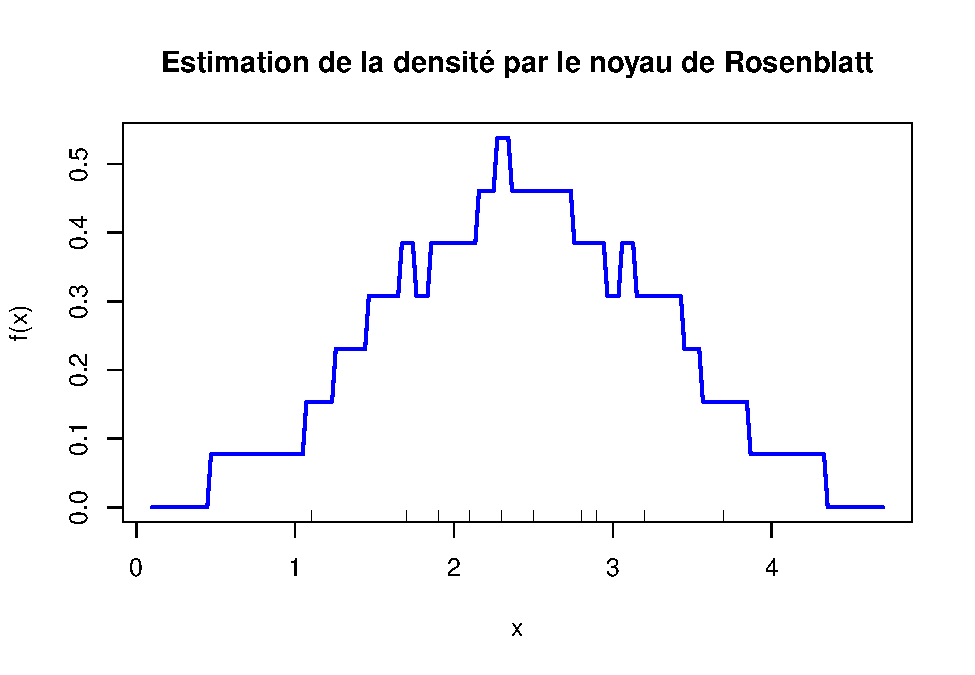
\includegraphics{Stat_non_para_files/figure-latex/unnamed-chunk-150-1.pdf}

\textbf{Avec une fonction native de R :} Il n'y pas de fonction native
de R permettant de calculer la densité avec le noyau de
Parzen-Rosenblatt.

\subsubsection{Noyau triangulaire}\label{noyau-triangulaire}

L'objectif ici , c'est d'estimer la densité de la loi de x à partir de
la méthode du noyau en utilisant le noyau triangulaire .

La densité estimée au point X est donnée par la forme ci-après :

\[
\hat{f}_h(x) = \frac{1}{n h} \sum_{i=1}^n K\left( \frac{x - X_i}{h} \right)
\]

avec \(K\) donné par :

\[
K(u) = (1 - |u|) \cdot \mathbb{1}_{\{|u| \leq 1\}}
\]

\begin{itemize}
\tightlist
\item
  \textbf{Fonction du noyau triangulaire}
\end{itemize}

\begin{Shaded}
\begin{Highlighting}[]
\NormalTok{triangular\_kernel }\OtherTok{\textless{}{-}} \ControlFlowTok{function}\NormalTok{(u) \{}
  \FunctionTok{ifelse}\NormalTok{(}\FunctionTok{abs}\NormalTok{(u) }\SpecialCharTok{\textless{}=} \DecValTok{1}\NormalTok{, }\DecValTok{1} \SpecialCharTok{{-}} \FunctionTok{abs}\NormalTok{(u), }\DecValTok{0}\NormalTok{)}
\NormalTok{\}}
\end{Highlighting}
\end{Shaded}

\begin{itemize}
\tightlist
\item
  \textbf{Fonction pour l'estimation de la densité aux points x}
\end{itemize}

\begin{Shaded}
\begin{Highlighting}[]
\CommentTok{\# Estimation de la densité aux points de x}
\NormalTok{estimate\_density\_x }\OtherTok{\textless{}{-}} \ControlFlowTok{function}\NormalTok{(x, h) \{}
\NormalTok{  n }\OtherTok{\textless{}{-}} \FunctionTok{length}\NormalTok{(x)}
\NormalTok{  f\_hat }\OtherTok{\textless{}{-}} \FunctionTok{numeric}\NormalTok{(n)}
  
  \ControlFlowTok{for}\NormalTok{ (i }\ControlFlowTok{in} \FunctionTok{seq\_along}\NormalTok{(x)) \{}
\NormalTok{    u }\OtherTok{\textless{}{-}}\NormalTok{ (x}\SpecialCharTok{{-}}\NormalTok{x[i]) }\SpecialCharTok{/}\NormalTok{ h}
\NormalTok{    f\_hat[i] }\OtherTok{\textless{}{-}} \FunctionTok{sum}\NormalTok{(}\FunctionTok{triangular\_kernel}\NormalTok{(u)) }\SpecialCharTok{/}\NormalTok{ (n }\SpecialCharTok{*}\NormalTok{ h)}
\NormalTok{  \}}
  
  \FunctionTok{return}\NormalTok{(f\_hat)}
\NormalTok{\}}
\end{Highlighting}
\end{Shaded}

\begin{itemize}
\tightlist
\item
  \textbf{Application de la fonction pour estimer la densité aux points
  de x}
\end{itemize}

Utilisons des données de l'exercice du cours :

\begin{Shaded}
\begin{Highlighting}[]
\CommentTok{\# Données}
\NormalTok{x }\OtherTok{\textless{}{-}} \FunctionTok{c}\NormalTok{(}\FloatTok{1.1}\NormalTok{, }\FloatTok{2.3}\NormalTok{, }\FloatTok{1.7}\NormalTok{,}\FloatTok{2.8}\NormalTok{, }\FloatTok{3.2}\NormalTok{, }\FloatTok{1.9}\NormalTok{, }\FloatTok{2.5}\NormalTok{, }\FloatTok{3.7}\NormalTok{, }\FloatTok{2.9}\NormalTok{, }\FloatTok{2.1}\NormalTok{)}
\end{Highlighting}
\end{Shaded}

\[
h = \frac{\max(x) - \min(x)}{\text{nombre de classes}}
\]

\begin{Shaded}
\begin{Highlighting}[]
\CommentTok{\# Nombre de classes}
\NormalTok{k }\OtherTok{\textless{}{-}} \DecValTok{4}

\CommentTok{\# Calcul de la fenêtre h}
\NormalTok{h }\OtherTok{\textless{}{-}}\NormalTok{ (}\FunctionTok{max}\NormalTok{(x) }\SpecialCharTok{{-}} \FunctionTok{min}\NormalTok{(x)) }\SpecialCharTok{/}\NormalTok{ k}

\CommentTok{\# Affichage}
\NormalTok{h}
\end{Highlighting}
\end{Shaded}

\begin{verbatim}
## [1] 0.65
\end{verbatim}

\begin{Shaded}
\begin{Highlighting}[]
\NormalTok{densities\_x }\OtherTok{\textless{}{-}} \FunctionTok{estimate\_density\_x}\NormalTok{(x, h)}

\NormalTok{resultats }\OtherTok{\textless{}{-}} \FunctionTok{data.frame}\NormalTok{(}
  \AttributeTok{x =}\NormalTok{ x,}
  \AttributeTok{densite\_estimee =}\NormalTok{ densities\_x}
\NormalTok{)}

\CommentTok{\# Affichage du tableau}
\NormalTok{resultats}
\end{Highlighting}
\end{Shaded}

\begin{verbatim}
##      x densite_estimee
## 1  1.1       0.1656805
## 2  2.3       0.4852071
## 3  1.7       0.3431953
## 4  2.8       0.4615385
## 5  3.2       0.3313609
## 6  1.9       0.4378698
## 7  2.5       0.4733728
## 8  3.7       0.1893491
## 9  2.9       0.4378698
## 10 2.1       0.4852071
\end{verbatim}

\subsubsection{Noyau Triweight}\label{noyau-triweight}

\begin{itemize}
\tightlist
\item
  \textbf{Estimation de densité}
\end{itemize}

L'estimateur à noyau de la densité est défini par :

\[\hat f_h(x) = \frac{1}{n\,h} \sum_{i=1}^n K\Bigl(\frac{x - X_i}{h}\Bigr),\]

avec :

\begin{itemize}
\item
  n la taille de l'échantillion
\item
  h la bande passante (paramétre de lissage)
\item
  K la fonction noyau
\end{itemize}

Le noyau de Triweight est défini par :

\[
K(u) = 
\begin{cases}
  \dfrac{35}{32}\,(1 - u^2)^3, & |u| \le 1, \\
  0, & |u| > 1.
\end{cases}
\]

\begin{itemize}
\tightlist
\item
  \textbf{Définition du noyau de Triweight : }
\end{itemize}

Syntaxe par defaut de R: bkde(estim\_notes, kernel = ``triweight'',
bandwidth = h) et h = bw.nrd0(estim\_notes), estimation de h par la
methode de Silverman Cette methode suppose que notre dataset suit une
loi normale.

\begin{Shaded}
\begin{Highlighting}[]
\NormalTok{triweight\_kernel }\OtherTok{\textless{}{-}} \ControlFlowTok{function}\NormalTok{(u) \{}
  \FunctionTok{ifelse}\NormalTok{(}\FunctionTok{abs}\NormalTok{(u) }\SpecialCharTok{\textless{}=} \DecValTok{1}\NormalTok{, (}\DecValTok{35}\SpecialCharTok{/}\DecValTok{32}\NormalTok{) }\SpecialCharTok{*}\NormalTok{ (}\DecValTok{1} \SpecialCharTok{{-}}\NormalTok{ u}\SpecialCharTok{\^{}}\DecValTok{2}\NormalTok{)}\SpecialCharTok{\^{}}\DecValTok{3}\NormalTok{, }\DecValTok{0}\NormalTok{)}
\NormalTok{\}}
\end{Highlighting}
\end{Shaded}

\begin{itemize}
\tightlist
\item
  \textbf{Fonction d'estimation}
\end{itemize}

\begin{Shaded}
\begin{Highlighting}[]
\NormalTok{density\_triweight }\OtherTok{\textless{}{-}} \ControlFlowTok{function}\NormalTok{(x0, X, h) \{}
\NormalTok{  u }\OtherTok{\textless{}{-}}\NormalTok{ (x0 }\SpecialCharTok{{-}}\NormalTok{ X) }\SpecialCharTok{/}\NormalTok{ h }\CommentTok{\# u est un vecteur}
  \FunctionTok{mean}\NormalTok{(}\FunctionTok{triweight\_kernel}\NormalTok{(u)) }\SpecialCharTok{/}\NormalTok{ h}
\NormalTok{\}}
\end{Highlighting}
\end{Shaded}

\begin{itemize}
\tightlist
\item
  \textbf{Visualisation de K(u) sur {[}-1.2,1.2{]}}
\end{itemize}

\begin{Shaded}
\begin{Highlighting}[]
\NormalTok{u }\OtherTok{\textless{}{-}} \FunctionTok{seq}\NormalTok{(}\SpecialCharTok{{-}}\FloatTok{1.2}\NormalTok{, }\FloatTok{1.2}\NormalTok{, }\AttributeTok{length.out =} \DecValTok{400}\NormalTok{) }\CommentTok{\# vecteur de 400 vleurs equidistant sur l\textquotesingle{}intervalle}
\FunctionTok{plot}\NormalTok{(u, }\FunctionTok{triweight\_kernel}\NormalTok{(u), }\AttributeTok{type =} \StringTok{\textquotesingle{}l\textquotesingle{}}\NormalTok{,}
     \AttributeTok{main =} \StringTok{\textquotesingle{}Noyau de Triweight\textquotesingle{}}\NormalTok{, }\AttributeTok{xlab =} \StringTok{\textquotesingle{}u\textquotesingle{}}\NormalTok{, }\AttributeTok{ylab =} \StringTok{\textquotesingle{}K(u)\textquotesingle{}}\NormalTok{)}
\end{Highlighting}
\end{Shaded}

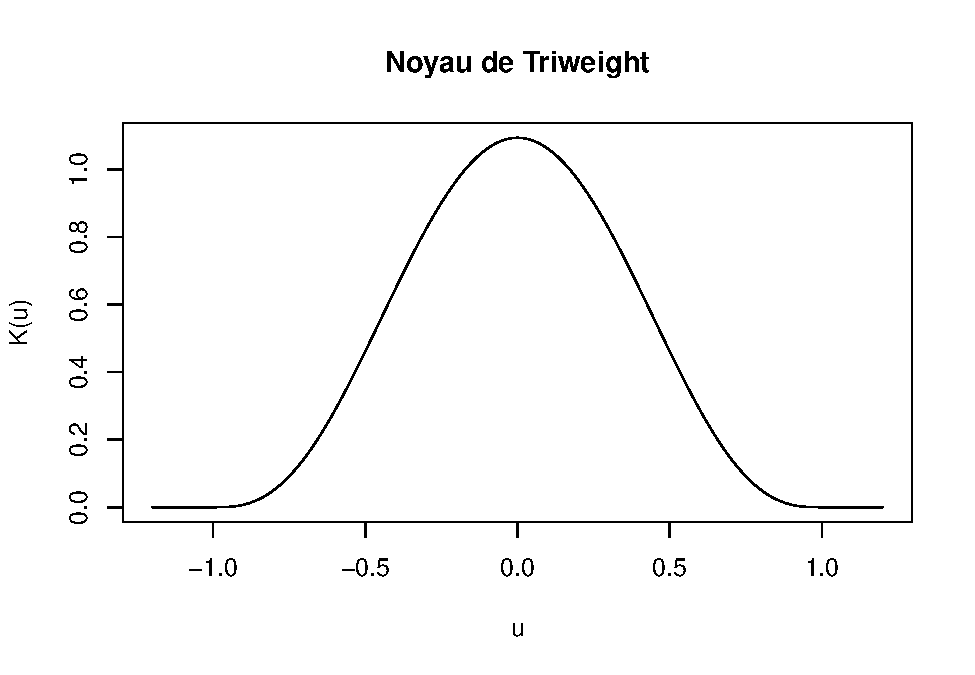
\includegraphics{Stat_non_para_files/figure-latex/unnamed-chunk-158-1.pdf}

\begin{Shaded}
\begin{Highlighting}[]
\NormalTok{data }\OtherTok{\textless{}{-}} \FunctionTok{read\_excel}\NormalTok{(}\StringTok{"BASES/notes\_Triweight\_kernel.xlsx"}\NormalTok{)}
\FunctionTok{head}\NormalTok{(data)}
\end{Highlighting}
\end{Shaded}

\begin{verbatim}
## # A tibble: 6 x 2
##   `Estimation/Moyenne` `Anthropo/Moyenne`
##                  <dbl>              <dbl>
## 1                  8                 16.5
## 2                 13                 14.5
## 3                  8                 15.5
## 4                 10                  8  
## 5                 10                 15  
## 6                  8.5               15
\end{verbatim}

\begin{Shaded}
\begin{Highlighting}[]
\NormalTok{estim\_notes }\OtherTok{\textless{}{-}}\NormalTok{ data[[}\DecValTok{1}\NormalTok{]]}
\NormalTok{anthrop\_notes }\OtherTok{\textless{}{-}}\NormalTok{ data[[}\DecValTok{2}\NormalTok{]]}
\end{Highlighting}
\end{Shaded}

\begin{itemize}
\tightlist
\item
  \textbf{Estimation de la densité}
\end{itemize}

ref:
\url{https://fastercapital.com/fr/contenu/La-regle-empirique-de-Silverman---une-regle-a-modeliser-par---les-connaissances-de-Silverman-sur-la-regression-du-noyau.html}

\[
h = 0.9 \cdot \min\left( \sigma, \frac{\text{IQR}}{1.34} \right) \cdot n^{-1/5}
\]

\begin{Shaded}
\begin{Highlighting}[]
\CommentTok{\# Grille d\textquotesingle{}evaluaton}
\NormalTok{grid }\OtherTok{\textless{}{-}} \FunctionTok{seq}\NormalTok{(}\FunctionTok{min}\NormalTok{(estim\_notes) }\SpecialCharTok{{-}} \DecValTok{1}\NormalTok{, }\FunctionTok{max}\NormalTok{(estim\_notes) }\SpecialCharTok{+} \DecValTok{1}\NormalTok{, }\AttributeTok{length.out =} \DecValTok{600}\NormalTok{) }

\CommentTok{\#print(grid)}

\CommentTok{\# Calcul de h par la régle empirique de Silverman\textquotesingle{}. }
\CommentTok{\# Le principe est de minimiser l\textquotesingle{}erreur quadratique moyenne (pour n grand, alors AMISE)}

\NormalTok{h\_theorique }\OtherTok{\textless{}{-}} \FloatTok{1.06} \SpecialCharTok{*} \FunctionTok{sd}\NormalTok{(estim\_notes) }\SpecialCharTok{*} \FunctionTok{length}\NormalTok{(estim\_notes)}\SpecialCharTok{\^{}}\NormalTok{(}\SpecialCharTok{{-}}\DecValTok{1}\SpecialCharTok{/}\DecValTok{5}\NormalTok{)}
\CommentTok{\# Ce h est la version theorique , elle est sensible aux outliers}


\CommentTok{\# En pratique on se sert d\textquotesingle{}une version plus robuste (c\textquotesingle{}est elle qui s\textquotesingle{}obtient avec bw.nrd0(estim\_notes))}
\CommentTok{\# car les données ne sont pas necessairement parfaitement normale donc possibilite de valeurs extremes}
\NormalTok{h\_silverman }\OtherTok{\textless{}{-}} \FloatTok{0.9} \SpecialCharTok{*} \FunctionTok{min}\NormalTok{(}\FunctionTok{sd}\NormalTok{(estim\_notes), }\FunctionTok{IQR}\NormalTok{(estim\_notes)}\SpecialCharTok{/}\FloatTok{1.34}\NormalTok{) }\SpecialCharTok{*} \FunctionTok{length}\NormalTok{(estim\_notes)}\SpecialCharTok{\^{}}\NormalTok{(}\SpecialCharTok{{-}}\DecValTok{1}\SpecialCharTok{/}\DecValTok{5}\NormalTok{)}

\FunctionTok{cat}\NormalTok{(}\StringTok{"h théorique (1.06 · σ · n\^{}({-}1/5)) :"}\NormalTok{, }\FunctionTok{round}\NormalTok{(h\_theorique, }\DecValTok{4}\NormalTok{), }\StringTok{"}\SpecialCharTok{\textbackslash{}n}\StringTok{"}\NormalTok{)}
\end{Highlighting}
\end{Shaded}

\begin{verbatim}
## h théorique (1.06 · σ · n^(-1/5)) : 0.9199
\end{verbatim}

\begin{Shaded}
\begin{Highlighting}[]
\FunctionTok{cat}\NormalTok{(}\StringTok{"h robuste (bw.nrd0)              :"}\NormalTok{, }\FunctionTok{round}\NormalTok{(h\_silverman, }\DecValTok{4}\NormalTok{), }\StringTok{"}\SpecialCharTok{\textbackslash{}n}\StringTok{"}\NormalTok{)}
\end{Highlighting}
\end{Shaded}

\begin{verbatim}
## h robuste (bw.nrd0)              : 0.781
\end{verbatim}

\begin{Shaded}
\begin{Highlighting}[]
\CommentTok{\# Calcul de l\textquotesingle{}estimation de tous les points}

\NormalTok{dens\_tri }\OtherTok{\textless{}{-}} \FunctionTok{sapply}\NormalTok{(grid, }\ControlFlowTok{function}\NormalTok{(x0) }\FunctionTok{density\_triweight}\NormalTok{(x0, }\AttributeTok{X =}\NormalTok{ estim\_notes, }\AttributeTok{h =}\NormalTok{ h\_silverman))}
\end{Highlighting}
\end{Shaded}

\begin{Shaded}
\begin{Highlighting}[]
\NormalTok{df }\OtherTok{\textless{}{-}} \FunctionTok{data.frame}\NormalTok{(}\AttributeTok{x =}\NormalTok{ grid, }\AttributeTok{dens =}\NormalTok{ dens\_tri)}
\FunctionTok{ggplot}\NormalTok{(df, }\FunctionTok{aes}\NormalTok{(}\AttributeTok{x =}\NormalTok{ x, }\AttributeTok{y =}\NormalTok{ dens)) }\SpecialCharTok{+}
  \FunctionTok{geom\_line}\NormalTok{(}\AttributeTok{size =} \DecValTok{1}\NormalTok{, }\AttributeTok{color =} \StringTok{\textquotesingle{}blue\textquotesingle{}}\NormalTok{) }\SpecialCharTok{+}
  \FunctionTok{labs}\NormalTok{(}
    \AttributeTok{title =} \StringTok{\textquotesingle{}Estimation de densité avec noyau de Triweight\textquotesingle{}}\NormalTok{,}
    \AttributeTok{subtitle =} \FunctionTok{paste}\NormalTok{(}\StringTok{\textquotesingle{}h =\textquotesingle{}}\NormalTok{, }\FunctionTok{round}\NormalTok{(h\_silverman, }\DecValTok{3}\NormalTok{)),}
    \AttributeTok{x =} \StringTok{\textquotesingle{}Valeurs\textquotesingle{}}\NormalTok{, }\AttributeTok{y =} \StringTok{\textquotesingle{}Densité estimée\textquotesingle{}}
\NormalTok{  ) }\SpecialCharTok{+}
  \FunctionTok{theme\_minimal}\NormalTok{()}
\end{Highlighting}
\end{Shaded}

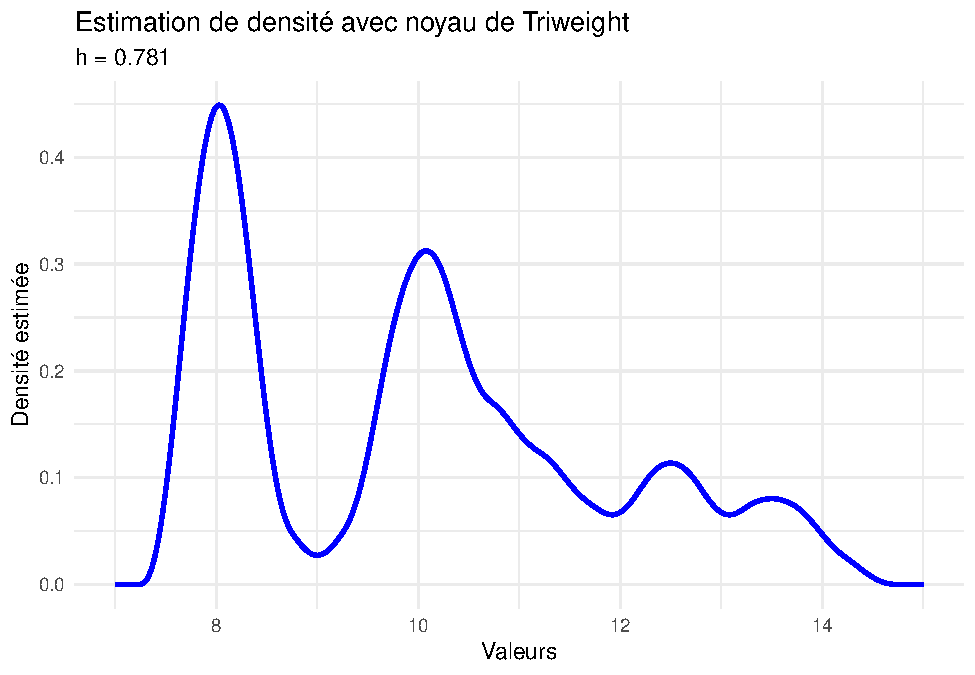
\includegraphics{Stat_non_para_files/figure-latex/unnamed-chunk-161-1.pdf}

\begin{itemize}
\tightlist
\item
  \textbf{Avec le package KernSmooth}
\end{itemize}

Par defaut, le noyau triweight n'est pas implementé dans la fonction
density,on se sert du package Par defaut, le noyau triweight n'est pas
implementé dans la fonction density. On se sert du package KernSmooth

\begin{Shaded}
\begin{Highlighting}[]
\NormalTok{h }\OtherTok{\textless{}{-}} \FunctionTok{bw.nrd0}\NormalTok{(estim\_notes)  }\CommentTok{\# methode de Silverman, argument par defaut dans la fonction density}
\FunctionTok{print}\NormalTok{(h)}
\end{Highlighting}
\end{Shaded}

\begin{verbatim}
## [1] 0.7810198
\end{verbatim}

\begin{Shaded}
\begin{Highlighting}[]
\NormalTok{res }\OtherTok{\textless{}{-}} \FunctionTok{bkde}\NormalTok{(estim\_notes, }\AttributeTok{kernel =} \StringTok{"triweight"}\NormalTok{, }\AttributeTok{bandwidth =}\NormalTok{ h)  }


\NormalTok{df\_kd }\OtherTok{\textless{}{-}} \FunctionTok{data.frame}\NormalTok{(}\AttributeTok{x =}\NormalTok{ res}\SpecialCharTok{$}\NormalTok{x, }\AttributeTok{y =}\NormalTok{ res}\SpecialCharTok{$}\NormalTok{y)}


\FunctionTok{ggplot}\NormalTok{(df\_kd, }\FunctionTok{aes}\NormalTok{(}\AttributeTok{x =}\NormalTok{ x, }\AttributeTok{y =}\NormalTok{ y)) }\SpecialCharTok{+}
  \FunctionTok{geom\_line}\NormalTok{(}\AttributeTok{color =} \StringTok{"darkorange"}\NormalTok{, }\AttributeTok{size =} \DecValTok{1}\NormalTok{) }\SpecialCharTok{+}
  \FunctionTok{labs}\NormalTok{(}
    \AttributeTok{title =} \StringTok{"Densité estimée (bkde) – noyau triweight"}\NormalTok{,}
    \AttributeTok{subtitle =} \FunctionTok{paste0}\NormalTok{(}\StringTok{"Bande passante (h) selon Silverman = "}\NormalTok{, }\FunctionTok{round}\NormalTok{(h, }\DecValTok{3}\NormalTok{)),}
    \AttributeTok{x =} \StringTok{"Valeurs"}\NormalTok{,}
    \AttributeTok{y =} \StringTok{"Densité"}
\NormalTok{  ) }\SpecialCharTok{+}
  \FunctionTok{theme\_minimal}\NormalTok{()}
\end{Highlighting}
\end{Shaded}

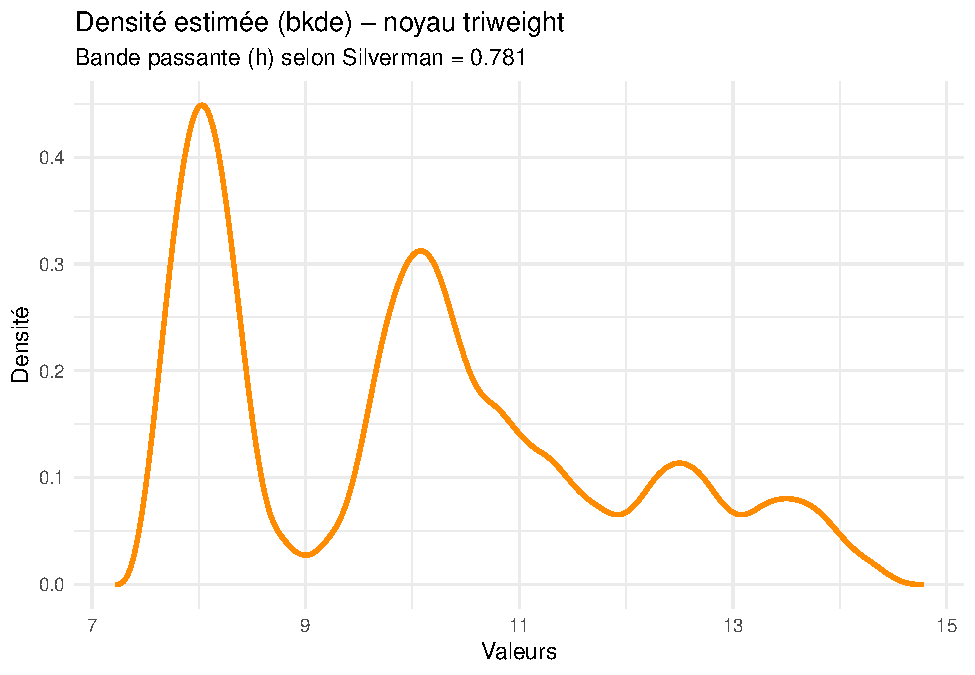
\includegraphics{Stat_non_para_files/figure-latex/unnamed-chunk-162-1.pdf}

\begin{Shaded}
\begin{Highlighting}[]
\CommentTok{\# df \textless{}{-} data.frame(x = grid, dens = dens\_tri)}

\FunctionTok{ggplot}\NormalTok{() }\SpecialCharTok{+}
  \CommentTok{\# Histogramme normalisé (les hauteurs correspondent a une densité)}
  \FunctionTok{geom\_histogram}\NormalTok{(}\FunctionTok{aes}\NormalTok{(}\AttributeTok{x =}\NormalTok{ estim\_notes, }\AttributeTok{y =} \FunctionTok{after\_stat}\NormalTok{(density)),}
                 \AttributeTok{bins =} \DecValTok{30}\NormalTok{, }\AttributeTok{fill =} \StringTok{"red"}\NormalTok{, }\AttributeTok{color =} \StringTok{"yellow"}\NormalTok{, }\AttributeTok{alpha =} \FloatTok{0.6}\NormalTok{) }\SpecialCharTok{+}
  
  \CommentTok{\# Courbe de densité estimée}
  \FunctionTok{geom\_line}\NormalTok{(}\AttributeTok{data =}\NormalTok{ df, }\FunctionTok{aes}\NormalTok{(}\AttributeTok{x =}\NormalTok{ x, }\AttributeTok{y =}\NormalTok{ dens),}
            \AttributeTok{color =} \StringTok{"blue"}\NormalTok{, }\AttributeTok{size =} \DecValTok{1}\NormalTok{) }\SpecialCharTok{+}
  
  \FunctionTok{labs}\NormalTok{(}
    \AttributeTok{title =} \StringTok{"Estimation de densité avec noyau de Triweight et histogramme"}\NormalTok{,}
    \AttributeTok{subtitle =} \FunctionTok{paste}\NormalTok{(}\StringTok{"h ="}\NormalTok{, }\FunctionTok{round}\NormalTok{(h\_silverman, }\DecValTok{3}\NormalTok{)),}
    \AttributeTok{x =} \StringTok{"Valeurs"}\NormalTok{,}
    \AttributeTok{y =} \StringTok{"Densité"}
\NormalTok{  ) }\SpecialCharTok{+}
  \FunctionTok{theme\_minimal}\NormalTok{()}
\end{Highlighting}
\end{Shaded}

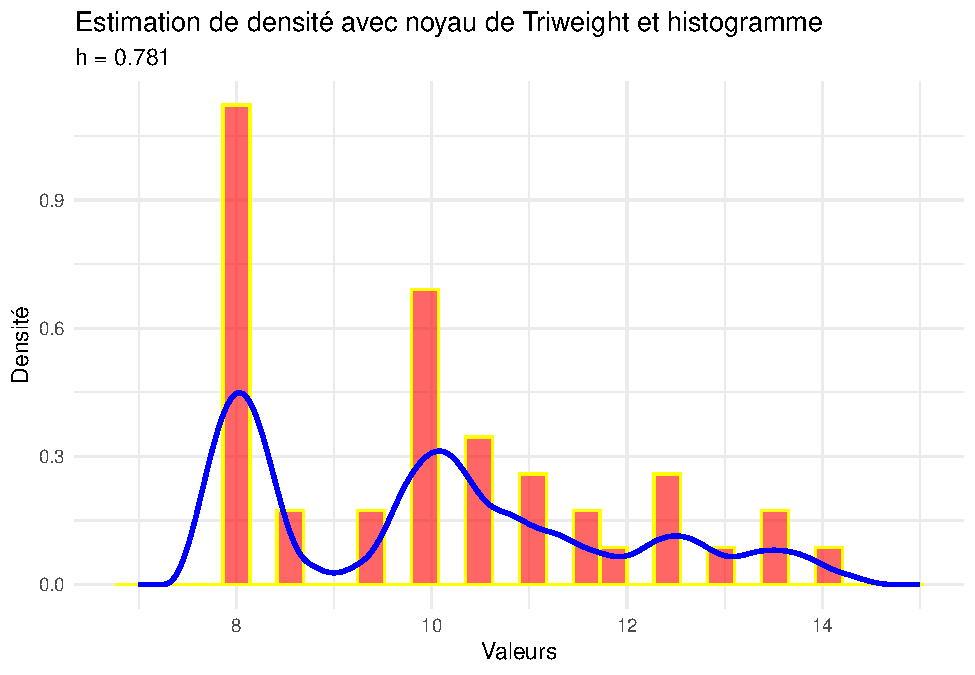
\includegraphics{Stat_non_para_files/figure-latex/unnamed-chunk-163-1.pdf}

\begin{itemize}
\tightlist
\item
  \textbf{Influence de la valeur de h}
\end{itemize}

\begin{Shaded}
\begin{Highlighting}[]
\NormalTok{h\_values }\OtherTok{\textless{}{-}} \FunctionTok{c}\NormalTok{(}\FloatTok{0.1}\NormalTok{, h\_silverman }\SpecialCharTok{/} \DecValTok{2}\NormalTok{, h\_silverman, }\DecValTok{2} \SpecialCharTok{*}\NormalTok{ h\_silverman)}
\CommentTok{\# Pour chaque valeur de h on créer un data frame puis on les merge tous.}

\NormalTok{df\_h }\OtherTok{\textless{}{-}} \FunctionTok{do.call}\NormalTok{(rbind, }\FunctionTok{lapply}\NormalTok{(h\_values, }\ControlFlowTok{function}\NormalTok{(h) \{}
\NormalTok{  dens }\OtherTok{\textless{}{-}} \FunctionTok{sapply}\NormalTok{(grid, }\ControlFlowTok{function}\NormalTok{(x0) }\FunctionTok{density\_triweight}\NormalTok{(x0, }\AttributeTok{X =}\NormalTok{ estim\_notes, }\AttributeTok{h =}\NormalTok{ h))}
  \FunctionTok{data.frame}\NormalTok{(}
    \AttributeTok{x    =}\NormalTok{ grid,}
    \AttributeTok{dens =}\NormalTok{ dens,}
    \AttributeTok{h    =} \FunctionTok{paste0}\NormalTok{(}\StringTok{\textquotesingle{}h = \textquotesingle{}}\NormalTok{, }\FunctionTok{round}\NormalTok{(h, }\DecValTok{3}\NormalTok{))}\CommentTok{\# arrondir a 3 chiffres}
\NormalTok{  )}
\NormalTok{\}))}

\FunctionTok{ggplot}\NormalTok{(df\_h, }\FunctionTok{aes}\NormalTok{(}\AttributeTok{x =}\NormalTok{ x, }\AttributeTok{y =}\NormalTok{ dens, }\AttributeTok{color =}\NormalTok{ h)) }\SpecialCharTok{+}
  \FunctionTok{geom\_line}\NormalTok{(}\AttributeTok{size =} \DecValTok{1}\NormalTok{) }\SpecialCharTok{+}
  \FunctionTok{labs}\NormalTok{(}
    \AttributeTok{title =} \StringTok{"  l\textquotesingle{}estimation de densité avec differents valeurs de h"}\NormalTok{,}
    \AttributeTok{x =} \StringTok{"Valeurs"}\NormalTok{, }\AttributeTok{y =} \StringTok{"Densité"}
\NormalTok{  ) }\SpecialCharTok{+}
  \FunctionTok{theme\_light}\NormalTok{()}
\end{Highlighting}
\end{Shaded}

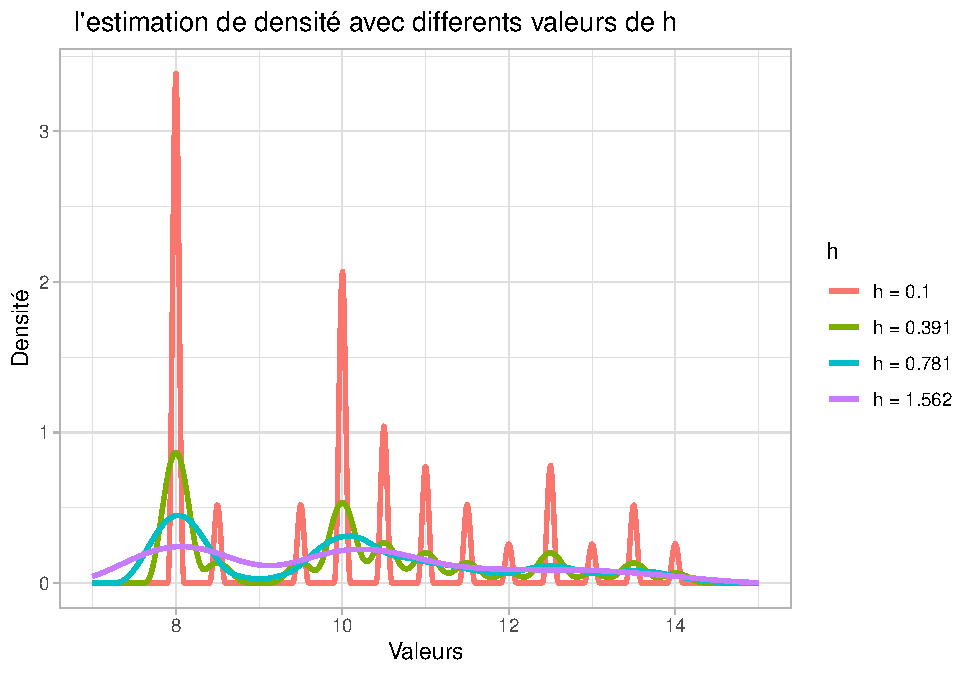
\includegraphics{Stat_non_para_files/figure-latex/unnamed-chunk-164-1.pdf}

\begin{itemize}
\tightlist
\item
  \textbf{Calcul de h par la methode AMISE}
\end{itemize}

Source :
\url{http://archives.univ-biskra.dz/bitstream/123456789/21522/1/Baia_Ikram.pdf}
, page 25

La formule asymptotique de l'erreur quadratique moyenne intégrée est :

\[
\text{AMISE}(h) \approx \frac{R(K)}{n h} + \frac{1}{4} h^4 \mu_2(K)^2 R(f'')
\]

Où :

\begin{itemize}
\tightlist
\item
  \[ R(K) = \int K^2(u)\,du )\]
\item
  \[ \mu_2(K) = \int u^2 K(u)\,du )\]
\item
  \[ R(f'') = \int [f''(x)]^2 dx )\]
\item
  n est la taille de l'échantillon La valeur de h qui minimise cette
  AMISE est :
\end{itemize}

\[
h_{\text{AMISE}} = \left( \frac{R(K)}{n \mu_2(K)^2 R(f'')} \right)^{1/5}
\]

Pour le noyau \textbf{Triweight} : - \[( R(K) = \frac{350}{429} )\] -
\[( \mu_2(K) = \frac{1}{9} )\]

R(f'\,') dépend de la vrai densité f qui est inconnue en pratique.

On approxime R(f'\,') sous l'hypothèse que les données suivent une
densité normale, auquel cas :

\[
R(f'') \approx \frac{3}{8 \sqrt{\pi} \sigma^5}
\]

où sigma est l'écart-type de l'échantillon.

\begin{Shaded}
\begin{Highlighting}[]
\NormalTok{R\_K }\OtherTok{\textless{}{-}} \DecValTok{350} \SpecialCharTok{/} \DecValTok{429}
\NormalTok{mu2\_K }\OtherTok{\textless{}{-}} \DecValTok{1} \SpecialCharTok{/} \DecValTok{9}

\CommentTok{\# Taille de l\textquotesingle{}échantillon et écart{-}type}

\NormalTok{n }\OtherTok{\textless{}{-}} \FunctionTok{length}\NormalTok{(estim\_notes)}
\NormalTok{sd\_X }\OtherTok{\textless{}{-}} \FunctionTok{sd}\NormalTok{(estim\_notes)}

\CommentTok{\# Approximation de R(f\textquotesingle{}\textquotesingle{}) sous hypothèse normale}

\NormalTok{Rf2 }\OtherTok{\textless{}{-}} \DecValTok{3} \SpecialCharTok{/}\NormalTok{ (}\DecValTok{8} \SpecialCharTok{*} \FunctionTok{sqrt}\NormalTok{(pi) }\SpecialCharTok{*}\NormalTok{ sd\_X}\SpecialCharTok{\^{}}\DecValTok{5}\NormalTok{)}


\NormalTok{h\_amise }\OtherTok{\textless{}{-}}\NormalTok{ (R\_K }\SpecialCharTok{/}\NormalTok{ (mu2\_K}\SpecialCharTok{\^{}}\DecValTok{2} \SpecialCharTok{*}\NormalTok{ Rf2 }\SpecialCharTok{*}\NormalTok{ n))}\SpecialCharTok{\^{}}\NormalTok{(}\DecValTok{1}\SpecialCharTok{/}\DecValTok{5}\NormalTok{)}
\FunctionTok{print}\NormalTok{(h\_amise)}
\end{Highlighting}
\end{Shaded}

\begin{verbatim}
## [1] 2.737458
\end{verbatim}

\begin{Shaded}
\begin{Highlighting}[]
\NormalTok{dens\_tri }\OtherTok{\textless{}{-}} \FunctionTok{sapply}\NormalTok{(grid, }\ControlFlowTok{function}\NormalTok{(x0) }\FunctionTok{density\_triweight}\NormalTok{(x0, }\AttributeTok{X =}\NormalTok{ estim\_notes, }\AttributeTok{h =}\NormalTok{ h\_amise))}
\NormalTok{df }\OtherTok{\textless{}{-}} \FunctionTok{data.frame}\NormalTok{(}\AttributeTok{x =}\NormalTok{ grid, }\AttributeTok{dens =}\NormalTok{ dens\_tri)}
\FunctionTok{ggplot}\NormalTok{() }\SpecialCharTok{+}
  \FunctionTok{geom\_histogram}\NormalTok{(}\FunctionTok{aes}\NormalTok{(}\AttributeTok{x =}\NormalTok{ estim\_notes, }\AttributeTok{y =} \FunctionTok{after\_stat}\NormalTok{(density)),}
                 \AttributeTok{bins =} \DecValTok{30}\NormalTok{, }\AttributeTok{fill =} \StringTok{"red"}\NormalTok{, }\AttributeTok{color =} \StringTok{"yellow"}\NormalTok{, }\AttributeTok{alpha =} \FloatTok{0.6}\NormalTok{) }\SpecialCharTok{+}
  \FunctionTok{geom\_line}\NormalTok{(}\AttributeTok{data =}\NormalTok{ df, }\FunctionTok{aes}\NormalTok{(}\AttributeTok{x =}\NormalTok{ x, }\AttributeTok{y =}\NormalTok{ dens),}
            \AttributeTok{color =} \StringTok{"blue"}\NormalTok{, }\AttributeTok{size =} \DecValTok{1}\NormalTok{) }\SpecialCharTok{+}
  \FunctionTok{labs}\NormalTok{(}
    \AttributeTok{title =} \StringTok{"Estimation de densité avec noyau Triweight"}\NormalTok{,}
    \AttributeTok{subtitle =} \FunctionTok{paste}\NormalTok{(}\StringTok{"h optimisé par AMISE .h ="}\NormalTok{, }\FunctionTok{round}\NormalTok{(h\_amise, }\DecValTok{3}\NormalTok{)),}
    \AttributeTok{x =} \StringTok{"Valeurs"}\NormalTok{, }\AttributeTok{y =} \StringTok{"Densité"}
\NormalTok{  ) }\SpecialCharTok{+}
  \FunctionTok{theme\_minimal}\NormalTok{()}
\end{Highlighting}
\end{Shaded}

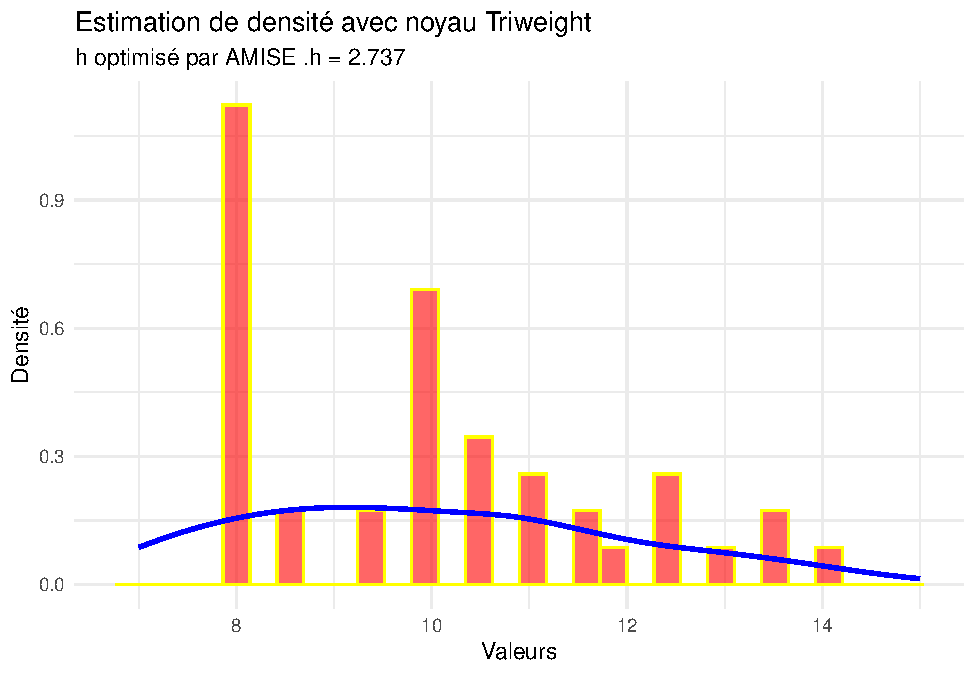
\includegraphics{Stat_non_para_files/figure-latex/unnamed-chunk-166-1.pdf}

Le choix de h relativement grand a pour effet de produire une courbe
très lisse, qui atténue les pics de l'histogramme.

\begin{itemize}
\tightlist
\item
  \textbf{Estimation de h par cross-validation par maximum de
  vraisemblance}
\end{itemize}

Son incovénient nous le verrons c'est le temps de calcul.

Source :
\url{https://cran.opencpu.org/web/packages/kedd/vignettes/kedd.pdf} ,
Page 9

La vraisemblance des données sous KDE est :

\[
L(h) = \prod_{i=1}^n \hat{f_h}(X_i)
\]

En prenant le logarithme, on obtient :

\[
\log L(h) = \sum_{i=1}^n \log \hat{f_h}(X_i)
\]

où \(\hat{f_h}(X_i)\) est l'estimation de la densité en \(X_i\) avec le
paramètre de lissage \(h\).

\begin{itemize}
\tightlist
\item
  \textbf{Problème de surapprentissage}
\end{itemize}

Lorsque \(h \to 0\), on a :

\[
\hat{f_h}(X_i) \to \infty
\]\\

Pour u\textgreater1, K(u) est nulle donc pour i différent de j, K((X\_i
- X\_j)/h) ==\textgreater0 mais comme K(0)\textgreater0 alors
1/(nh)*K(0)==\textgreater{} + infini chaque observation contribue
fortement à sa propre estimation (graphiquement on obtient des pics sur
les points connus). Cela conduit à un sur-apprentissage .

Cela pousserait l'algorithme à choisir un h arbitrairement petit,
conduisant à un sur-apprentissage extrême où la densité estimée serait
une série de pics infinitésimaux à chaque point de donnée.

Pour éviter ce problème, on utilise la cross-validation par maximum de
vraisemblance.

On estime la densité en excluant successivement chaque observation
\(X_i\).

L'estimateur de la densité en \(X_i\) excluant \(X_i\) est donné par :

\[
\hat{f_{h,-i}}(X_i) = \frac{1}{(n-1)h} \sum_{j \ne i} K\left(\frac{X_i - X_j}{h}\right)
\]

La log-vraisemblance devient : \[
CV(h) = \frac{1}{n} \sum_{i=1}^n \log \hat{f_{h,-i}}(X_i)
\]

ce critère de CV converge en probabilité vers la MISE:
\url{https://www.researchgate.net/publication/280609040_Bootstrap_dans_l\%27estimation_de_la_densite_par_la_methode_du_noyau}

\[
{h}_{CV} = \arg\max_{h > 0} CV(h)
\]

Cette méthode est non paramétrique et ne suppose aucune hypothèse forte
sur la forme de la densité, tout en évitant le sur-apprentissage.

\begin{Shaded}
\begin{Highlighting}[]
\CommentTok{\# Fonction de cross{-}validation}

\NormalTok{cv\_log\_likelihood }\OtherTok{\textless{}{-}} \ControlFlowTok{function}\NormalTok{(h, X) \{}
\NormalTok{  n }\OtherTok{\textless{}{-}} \FunctionTok{length}\NormalTok{(X)}
\NormalTok{  log\_dens }\OtherTok{\textless{}{-}} \FunctionTok{sapply}\NormalTok{(}\DecValTok{1}\SpecialCharTok{:}\NormalTok{n, }\ControlFlowTok{function}\NormalTok{(i) \{}
\NormalTok{    xi }\OtherTok{\textless{}{-}}\NormalTok{ X[i]}
\NormalTok{    x\_others }\OtherTok{\textless{}{-}}\NormalTok{ X[}\SpecialCharTok{{-}}\NormalTok{i]}
\NormalTok{    u }\OtherTok{\textless{}{-}}\NormalTok{ (xi }\SpecialCharTok{{-}}\NormalTok{ x\_others) }\SpecialCharTok{/}\NormalTok{ h}
\NormalTok{    k\_vals }\OtherTok{\textless{}{-}} \FunctionTok{triweight\_kernel}\NormalTok{(u)}
\NormalTok{    f\_hat }\OtherTok{\textless{}{-}} \FunctionTok{mean}\NormalTok{(k\_vals) }\SpecialCharTok{/}\NormalTok{ h}
    \FunctionTok{log}\NormalTok{(f\_hat)}
\NormalTok{  \})}
  \SpecialCharTok{{-}}\FunctionTok{mean}\NormalTok{(log\_dens) }\CommentTok{\# Le signe {-} car en pratique on prend l\textquotesingle{}oppose de CV ( On minimise)}
\NormalTok{\}}
\end{Highlighting}
\end{Shaded}

A present pour trouver le h optimal il nous faut des candidats

\begin{Shaded}
\begin{Highlighting}[]
\CommentTok{\# Séquence de valeurs pour h à tester 100 valeurs}
\NormalTok{h\_seq }\OtherTok{\textless{}{-}} \FunctionTok{seq}\NormalTok{(}\FloatTok{0.1}\NormalTok{, }\DecValTok{2}\NormalTok{, }\AttributeTok{length.out =} \DecValTok{100}\NormalTok{) }

\CommentTok{\# Application de la fonction (output list)}
\NormalTok{cv\_vals }\OtherTok{\textless{}{-}} \FunctionTok{sapply}\NormalTok{(h\_seq, }\ControlFlowTok{function}\NormalTok{(h) }\FunctionTok{cv\_log\_likelihood}\NormalTok{(h, estim\_notes))}

\CommentTok{\# Recherche de la valeur optimale de h}

\NormalTok{h\_cv }\OtherTok{\textless{}{-}}\NormalTok{ h\_seq[}\FunctionTok{which.min}\NormalTok{(cv\_vals)]}
\FunctionTok{cat}\NormalTok{(}\StringTok{"h optimal est:"}\NormalTok{, }\FunctionTok{round}\NormalTok{(h\_cv, }\DecValTok{4}\NormalTok{), }\StringTok{"}\SpecialCharTok{\textbackslash{}n}\StringTok{"}\NormalTok{)}
\end{Highlighting}
\end{Shaded}

\begin{verbatim}
## h optimal est: 0.8677
\end{verbatim}

\begin{Shaded}
\begin{Highlighting}[]
\CommentTok{\# Densité estimée avec h\_cv}
\NormalTok{dens\_cv }\OtherTok{\textless{}{-}} \FunctionTok{sapply}\NormalTok{(grid, }\ControlFlowTok{function}\NormalTok{(x0) }\FunctionTok{density\_triweight}\NormalTok{(x0, }\AttributeTok{X =}\NormalTok{ estim\_notes, }\AttributeTok{h =}\NormalTok{ h\_cv))}
\NormalTok{df\_cv }\OtherTok{\textless{}{-}} \FunctionTok{data.frame}\NormalTok{(}\AttributeTok{x =}\NormalTok{ grid, }\AttributeTok{dens =}\NormalTok{ dens\_cv)}

\FunctionTok{ggplot}\NormalTok{() }\SpecialCharTok{+}
  \FunctionTok{geom\_histogram}\NormalTok{(}\FunctionTok{aes}\NormalTok{(}\AttributeTok{x =}\NormalTok{ estim\_notes, }\AttributeTok{y =} \FunctionTok{after\_stat}\NormalTok{(density)),}
                 \AttributeTok{bins =} \DecValTok{30}\NormalTok{, }\AttributeTok{fill =} \StringTok{"red"}\NormalTok{, }\AttributeTok{color =} \StringTok{"yellow"}\NormalTok{, }\AttributeTok{alpha =} \FloatTok{0.5}\NormalTok{) }\SpecialCharTok{+}
  \FunctionTok{geom\_line}\NormalTok{(}\AttributeTok{data =}\NormalTok{ df\_cv, }\FunctionTok{aes}\NormalTok{(}\AttributeTok{x =}\NormalTok{ x, }\AttributeTok{y =}\NormalTok{ dens),}
            \AttributeTok{color =} \StringTok{"blue"}\NormalTok{, }\AttributeTok{size =} \FloatTok{1.2}\NormalTok{) }\SpecialCharTok{+}
  \FunctionTok{labs}\NormalTok{(}
    \AttributeTok{title =} \StringTok{"Estimation de densité avec noyau Triweight"}\NormalTok{,}
    \AttributeTok{subtitle =} \FunctionTok{paste}\NormalTok{(}\StringTok{"h optimisé par cross{-}validation ="}\NormalTok{, }\FunctionTok{round}\NormalTok{(h\_cv, }\DecValTok{3}\NormalTok{)),}
    \AttributeTok{x =} \StringTok{"Valeurs"}\NormalTok{, }\AttributeTok{y =} \StringTok{"Densité"}
\NormalTok{  ) }\SpecialCharTok{+}
  \FunctionTok{theme\_minimal}\NormalTok{()}
\end{Highlighting}
\end{Shaded}

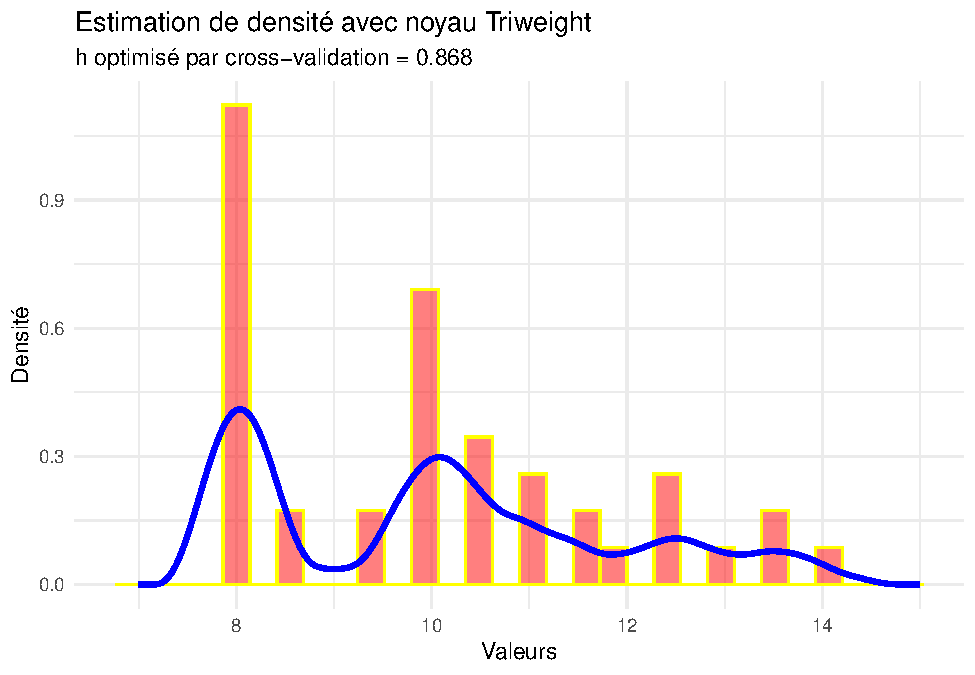
\includegraphics{Stat_non_para_files/figure-latex/unnamed-chunk-169-1.pdf}

\textbf{Lien avec la MISE :} Il a été montré que la minimisation de ce
critère de validation croisée est asymptotiquement équivalente à la
minimisation de la MISE.

\subsubsection{Noyau du cosinus}\label{noyau-du-cosinus}

Le noyau cosinus est donné par :

\[K(t) = \frac{\pi}{4} \cos\left(\frac{\pi}{2} t\right) \mathbf{1}_{[-1,1]}(t)\]
Le code R pour la fonction est le suivant :

\begin{Shaded}
\begin{Highlighting}[]
\NormalTok{K }\OtherTok{\textless{}{-}} \ControlFlowTok{function}\NormalTok{(x)}
\NormalTok{  \{}
\NormalTok{  K }\OtherTok{\textless{}{-}} \DecValTok{0}
  \ControlFlowTok{if}\NormalTok{ (}\SpecialCharTok{{-}}\DecValTok{1} \SpecialCharTok{\textless{}=}\NormalTok{ x }\SpecialCharTok{\&\&}\NormalTok{ x }\SpecialCharTok{\textless{}=} \DecValTok{1}\NormalTok{) \{}
\NormalTok{    K }\OtherTok{\textless{}{-}}\NormalTok{ (pi}\SpecialCharTok{/}\DecValTok{4}\NormalTok{)}\SpecialCharTok{*}\FunctionTok{cos}\NormalTok{(x}\SpecialCharTok{*}\NormalTok{pi}\SpecialCharTok{/}\DecValTok{2}\NormalTok{)}
\NormalTok{  \} }
  \FunctionTok{return}\NormalTok{ (K)}
\NormalTok{\}}
\end{Highlighting}
\end{Shaded}

\begin{itemize}
\tightlist
\item
  \textbf{Test}
\end{itemize}

\begin{Shaded}
\begin{Highlighting}[]
\FunctionTok{print}\NormalTok{(}\FunctionTok{K}\NormalTok{(}\DecValTok{0}\NormalTok{))}
\end{Highlighting}
\end{Shaded}

\begin{verbatim}
## [1] 0.7853982
\end{verbatim}

\begin{itemize}
\tightlist
\item
  \textbf{L'estimateur de densité}
\end{itemize}

L'estimateur de densité moyennant le noyau cosinus est donné par :

\[\hat{f}_n(x) = \frac{1}{n h} \sum_{i=1}^n \frac{\pi}{4} \cos\left(\frac{\pi}{2} \frac{x - x_i}{h}\right) \mathbf{1}_{[-1,1]}\left(\frac{x - x_i}{h}\right)\]

Le code R est le suivant :

\begin{Shaded}
\begin{Highlighting}[]
\NormalTok{fn }\OtherTok{\textless{}{-}} \ControlFlowTok{function}\NormalTok{(data,x,nb\_cla)\{}
\NormalTok{  n }\OtherTok{\textless{}{-}} \FunctionTok{length}\NormalTok{(data)}
\NormalTok{  h }\OtherTok{\textless{}{-}}\NormalTok{ (}\FunctionTok{max}\NormalTok{(data)}\SpecialCharTok{{-}}\FunctionTok{min}\NormalTok{(data))}\SpecialCharTok{/}\NormalTok{nb\_cla}
\NormalTok{  fn }\OtherTok{\textless{}{-}} \DecValTok{0}
  \ControlFlowTok{for}\NormalTok{ (i }\ControlFlowTok{in} \DecValTok{1}\SpecialCharTok{:}\NormalTok{n)\{}
\NormalTok{    fn }\OtherTok{\textless{}{-}}\NormalTok{ fn }\SpecialCharTok{+} \FunctionTok{K}\NormalTok{((x}\SpecialCharTok{{-}}\NormalTok{data[i])}\SpecialCharTok{/}\NormalTok{h)}
\NormalTok{  \}}
\NormalTok{  fn }\OtherTok{\textless{}{-}}\NormalTok{ fn}\SpecialCharTok{/}\NormalTok{(n}\SpecialCharTok{*}\NormalTok{h)}
  \FunctionTok{return}\NormalTok{ (fn)}
\NormalTok{\}}
\end{Highlighting}
\end{Shaded}

\begin{itemize}
\tightlist
\item
  \textbf{Test- }
\end{itemize}

\begin{Shaded}
\begin{Highlighting}[]
\NormalTok{data }\OtherTok{\textless{}{-}} \FunctionTok{c}\NormalTok{(}\FloatTok{1.1}\NormalTok{,}\FloatTok{2.3}\NormalTok{,}\FloatTok{1.7}\NormalTok{,}\FloatTok{2.8}\NormalTok{,}\FloatTok{3.2}\NormalTok{,}\FloatTok{1.9}\NormalTok{,}\FloatTok{2.5}\NormalTok{,}\FloatTok{3.7}\NormalTok{,}\FloatTok{2.9}\NormalTok{,}\FloatTok{2.1}\NormalTok{)}

\CommentTok{\# Test de la fonction au point x = 1.1}
\FunctionTok{print}\NormalTok{(}\FunctionTok{fn}\NormalTok{(}\AttributeTok{data =}\NormalTok{ data,}\AttributeTok{x =} \FloatTok{1.1}\NormalTok{,}\AttributeTok{nb\_cla =} \DecValTok{4}\NormalTok{))}
\end{Highlighting}
\end{Shaded}

\begin{verbatim}
## [1] 0.135395
\end{verbatim}

\begin{itemize}
\tightlist
\item
  \textbf{Application sur des données réelles de l'EHCVM}
\end{itemize}

Nous allons maintenant donner une application concrète sur les données
EHCVM.

\begin{Shaded}
\begin{Highlighting}[]
\NormalTok{ehcvm\_welfare\_sen2018 }\OtherTok{\textless{}{-}} \FunctionTok{read\_dta}\NormalTok{(}\StringTok{"BASES/ehcvm\_welfare\_sen2018.dta"}\NormalTok{)}
\FunctionTok{head}\NormalTok{(ehcvm\_welfare\_sen2018)}
\end{Highlighting}
\end{Shaded}

\begin{verbatim}
## # A tibble: 6 x 35
##   country  year  hhid grappe menage vague   zae region   milieu  hhweight hhsize
##   <chr>   <dbl> <dbl>  <dbl>  <dbl> <dbl> <dbl> <dbl+lb> <dbl+l>    <dbl>  <dbl>
## 1 SEN      2018  1001      1      1     1     1 1 [daka~ 1 [Urb~    1750.      2
## 2 SEN      2018  1002      1      2     1     1 1 [daka~ 1 [Urb~    1750.      2
## 3 SEN      2018  1003      1      3     1     1 1 [daka~ 1 [Urb~    1750.      1
## 4 SEN      2018  2001      2      1     2     1 1 [daka~ 1 [Urb~     266.     10
## 5 SEN      2018  2002      2      2     2     1 1 [daka~ 1 [Urb~     266.      6
## 6 SEN      2018  2003      2      3     2     1 1 [daka~ 1 [Urb~     266.      4
## # i 24 more variables: eqadu1 <dbl>, eqadu2 <dbl>, hgender <dbl+lbl>,
## #   hage <dbl>, hmstat <dbl+lbl>, hreligion <dbl+lbl>, hnation <dbl+lbl>,
## #   halfab <dbl+lbl>, heduc <dbl+lbl>, hdiploma <dbl+lbl>, hhandig <dbl+lbl>,
## #   hactiv7j <dbl+lbl>, hactiv12m <dbl+lbl>, hbranch <dbl+lbl>,
## #   hsectins <dbl+lbl>, hcsp <dbl+lbl>, dali <dbl>, dnal <dbl>, dtot <dbl>,
## #   pcexp <dbl>, zzae <dbl>, zref <dbl>, def_spa <dbl>, def_temp <dbl>
\end{verbatim}

\begin{Shaded}
\begin{Highlighting}[]
\NormalTok{data }\OtherTok{\textless{}{-}} \FunctionTok{as.vector}\NormalTok{(ehcvm\_welfare\_sen2018}\SpecialCharTok{$}\NormalTok{pcexp)}
\end{Highlighting}
\end{Shaded}

\begin{itemize}
\tightlist
\item
  \textbf{Représentation de l'histogramme des données}
\end{itemize}

\begin{Shaded}
\begin{Highlighting}[]
\FunctionTok{hist}\NormalTok{(data, }\AttributeTok{breaks =} \DecValTok{200}\NormalTok{,}\AttributeTok{freq =} \ConstantTok{FALSE}\NormalTok{, }\AttributeTok{main =} \StringTok{"Histogramme des dépenses de consommation par tête (pcexp)"}\NormalTok{, }\AttributeTok{xlab =} \StringTok{"Dépense"}\NormalTok{)}

\NormalTok{x\_vals }\OtherTok{\textless{}{-}} \FunctionTok{seq}\NormalTok{(}\FunctionTok{min}\NormalTok{(data), }\FunctionTok{max}\NormalTok{(data), }\AttributeTok{length.out =} \DecValTok{200}\NormalTok{)}
\NormalTok{f\_vals }\OtherTok{\textless{}{-}} \FunctionTok{sapply}\NormalTok{(x\_vals, }\ControlFlowTok{function}\NormalTok{(x) }\FunctionTok{fn}\NormalTok{(data, x , }\AttributeTok{nb\_cla =} \DecValTok{200}\NormalTok{))}
\FunctionTok{lines}\NormalTok{(x\_vals, f\_vals, }\AttributeTok{col =} \StringTok{"blue"}\NormalTok{, }\AttributeTok{lwd =} \DecValTok{2}\NormalTok{)}
\FunctionTok{legend}\NormalTok{(}\StringTok{"topright"}\NormalTok{, }\AttributeTok{legend =} \FunctionTok{c}\NormalTok{(}\StringTok{"Densité estimée"}\NormalTok{), }\AttributeTok{col =} \FunctionTok{c}\NormalTok{(}\StringTok{"blue"}\NormalTok{), }\AttributeTok{lwd =} \DecValTok{2}\NormalTok{, }\AttributeTok{lty =} \FunctionTok{c}\NormalTok{(}\DecValTok{1}\NormalTok{, }\DecValTok{2}\NormalTok{))}
\end{Highlighting}
\end{Shaded}

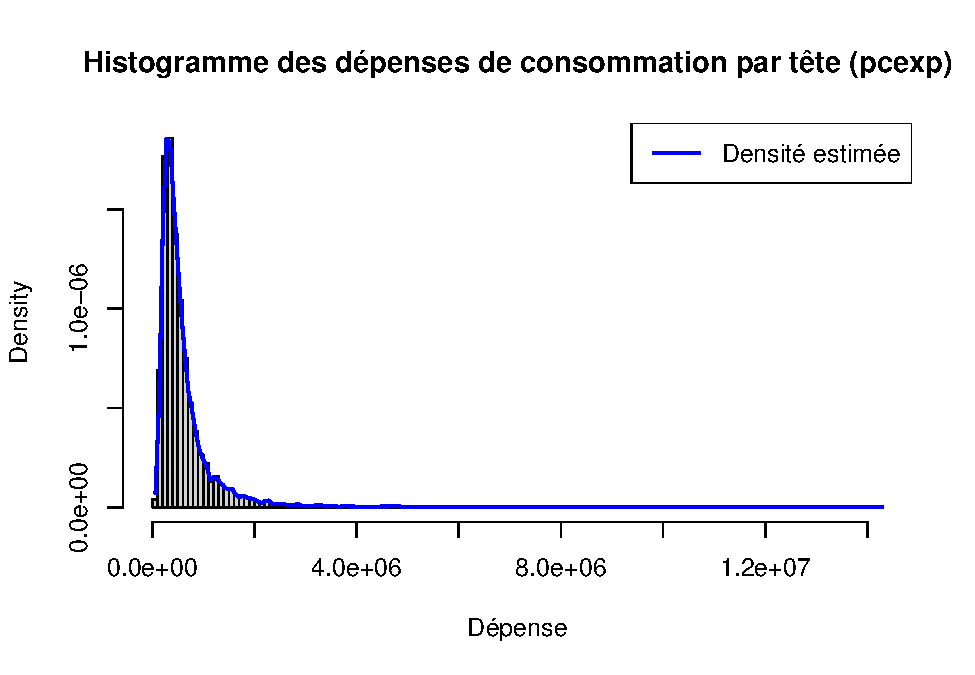
\includegraphics{Stat_non_para_files/figure-latex/unnamed-chunk-176-1.pdf}

\begin{itemize}
\tightlist
\item
  \textbf{Estimation de la densité avec la fonction density()}
\end{itemize}

Nous utilisons maintenant la fonction prédéfinie dans R pour comparer à
la notre.

\begin{Shaded}
\begin{Highlighting}[]
\CommentTok{\# Créer l\textquotesingle{}histogramme de base}
\FunctionTok{hist}\NormalTok{(data, }\AttributeTok{breaks =} \DecValTok{200}\NormalTok{, }\AttributeTok{freq =} \ConstantTok{FALSE}\NormalTok{, }
     \AttributeTok{main =} \StringTok{"Histogramme des dépenses de consommation par tête (pcexp)"}\NormalTok{, }
     \AttributeTok{xlab =} \StringTok{"Dépense"}\NormalTok{, }\AttributeTok{col =} \StringTok{"lightgray"}\NormalTok{)}

\CommentTok{\# Première courbe}
\NormalTok{x\_vals }\OtherTok{\textless{}{-}} \FunctionTok{seq}\NormalTok{(}\FunctionTok{min}\NormalTok{(data), }\FunctionTok{max}\NormalTok{(data), }\AttributeTok{length.out =} \DecValTok{200}\NormalTok{)}
\NormalTok{f\_vals }\OtherTok{\textless{}{-}} \FunctionTok{sapply}\NormalTok{(x\_vals, }\ControlFlowTok{function}\NormalTok{(x) }\FunctionTok{fn}\NormalTok{(data, x, }\AttributeTok{nb\_cla =} \DecValTok{200}\NormalTok{))}
\FunctionTok{lines}\NormalTok{(x\_vals, f\_vals, }\AttributeTok{col =} \StringTok{"blue"}\NormalTok{, }\AttributeTok{lwd =} \DecValTok{2}\NormalTok{)}

\CommentTok{\# Deuxième courbe}
\NormalTok{dens }\OtherTok{\textless{}{-}} \FunctionTok{density}\NormalTok{(data, }\AttributeTok{kernel =} \StringTok{"cosine"}\NormalTok{, }\AttributeTok{n =} \DecValTok{200}\NormalTok{)}
\FunctionTok{lines}\NormalTok{(dens}\SpecialCharTok{$}\NormalTok{x, dens}\SpecialCharTok{$}\NormalTok{y, }\AttributeTok{col =} \StringTok{"red"}\NormalTok{, }\AttributeTok{lwd =} \DecValTok{2}\NormalTok{)}

\CommentTok{\# Légende}
\FunctionTok{legend}\NormalTok{(}\StringTok{"topright"}\NormalTok{, }
       \AttributeTok{legend =} \FunctionTok{c}\NormalTok{(}\StringTok{"Densité estimée (méthode 1)"}\NormalTok{, }\StringTok{"Densité estimée par la fonction density()"}\NormalTok{), }
       \AttributeTok{col =} \FunctionTok{c}\NormalTok{(}\StringTok{"blue"}\NormalTok{, }\StringTok{"red"}\NormalTok{), }\AttributeTok{lwd =} \DecValTok{2}\NormalTok{, }\AttributeTok{lty =} \DecValTok{1}\NormalTok{)}
\end{Highlighting}
\end{Shaded}

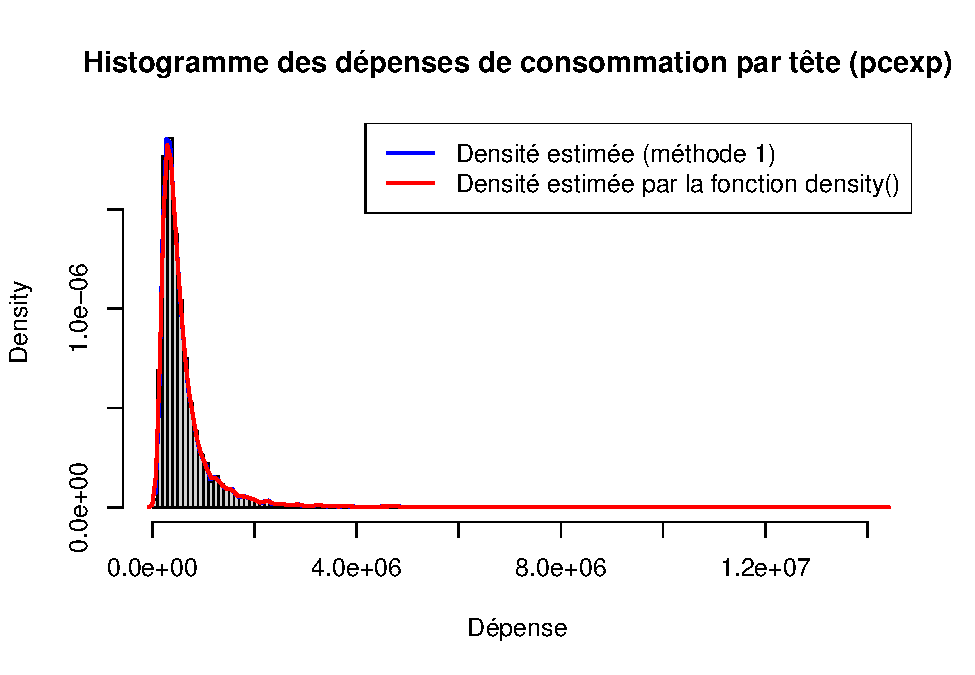
\includegraphics{Stat_non_para_files/figure-latex/unnamed-chunk-177-1.pdf}

On constate qu'on a pratiquement les mêmes résultats.

\begin{itemize}
\tightlist
\item
  \textbf{Cas de la mesure de pauvreté}
\end{itemize}

L'objectif ici est d'approximer la densité de la loi des dépenses de
consommation par tête (variable pcexp) et de déterminer le taux de
pauvreté.

\begin{itemize}
\tightlist
\item
  \textbf{Taux de pauvreté (aire sous la densité à gauche du seuil z)}
\end{itemize}

\begin{Shaded}
\begin{Highlighting}[]
\NormalTok{z }\OtherTok{\textless{}{-}} \FunctionTok{mean}\NormalTok{(ehcvm\_welfare\_sen2018}\SpecialCharTok{$}\NormalTok{zref)}
\NormalTok{dens\_vals }\OtherTok{\textless{}{-}} \FunctionTok{sapply}\NormalTok{(data, }\ControlFlowTok{function}\NormalTok{(xi) }\FunctionTok{as.numeric}\NormalTok{(xi }\SpecialCharTok{\textless{}}\NormalTok{ z))}
\end{Highlighting}
\end{Shaded}

\begin{itemize}
\tightlist
\item
  \textbf{Construction}
\end{itemize}

\begin{Shaded}
\begin{Highlighting}[]
\FunctionTok{hist}\NormalTok{(data, }\AttributeTok{breaks =} \DecValTok{200}\NormalTok{, }\AttributeTok{freq =} \ConstantTok{FALSE}\NormalTok{,}
     \AttributeTok{main =} \StringTok{"Analyse de la pauvreté"}\NormalTok{,}
     \AttributeTok{xlab =} \StringTok{"Dépenses de consommation par tête"}\NormalTok{,}
     \AttributeTok{col =} \StringTok{"blue"}\NormalTok{, }\AttributeTok{border =} \StringTok{"white"}\NormalTok{)}

\CommentTok{\# Tracer la densité}
\FunctionTok{lines}\NormalTok{(x\_vals, f\_vals, }\AttributeTok{col =} \StringTok{"green"}\NormalTok{, }\AttributeTok{lwd =} \DecValTok{2}\NormalTok{)}


\CommentTok{\# Colorier l\textquotesingle{}aire sous la courbe avant le seuil z}
\NormalTok{polygon\_x }\OtherTok{\textless{}{-}}\NormalTok{ x\_vals[x\_vals }\SpecialCharTok{\textless{}=}\NormalTok{ z]}
\NormalTok{polygon\_y }\OtherTok{\textless{}{-}}\NormalTok{ f\_vals[x\_vals }\SpecialCharTok{\textless{}=}\NormalTok{ z]}
\FunctionTok{polygon}\NormalTok{(}\FunctionTok{c}\NormalTok{(polygon\_x, }\FunctionTok{rev}\NormalTok{(polygon\_x)), }\FunctionTok{c}\NormalTok{(}\FunctionTok{rep}\NormalTok{(}\DecValTok{0}\NormalTok{, }\FunctionTok{length}\NormalTok{(polygon\_x)), }\FunctionTok{rev}\NormalTok{(polygon\_y)),}
        \AttributeTok{col =} \StringTok{"red"}\NormalTok{, }\AttributeTok{border =} \ConstantTok{NA}\NormalTok{)}

\CommentTok{\# Ligne verticale pour le seuil}
\FunctionTok{abline}\NormalTok{(}\AttributeTok{v =}\NormalTok{ z, }\AttributeTok{col =} \StringTok{"blue"}\NormalTok{, }\AttributeTok{lwd =} \DecValTok{2}\NormalTok{, }\AttributeTok{lty =} \DecValTok{2}\NormalTok{)}

\CommentTok{\# Calcul du taux de pauvreté}
\NormalTok{z }\OtherTok{\textless{}{-}} \FunctionTok{mean}\NormalTok{(ehcvm\_welfare\_sen2018}\SpecialCharTok{$}\NormalTok{zref)}
\NormalTok{poid}\OtherTok{=}\NormalTok{ehcvm\_welfare\_sen2018}\SpecialCharTok{$}\NormalTok{hhweight}\SpecialCharTok{*}\NormalTok{ehcvm\_welfare\_sen2018}\SpecialCharTok{$}\NormalTok{hhsize}\SpecialCharTok{/}\FunctionTok{sum}\NormalTok{(ehcvm\_welfare\_sen2018}\SpecialCharTok{$}\NormalTok{hhweight}\SpecialCharTok{*}\NormalTok{ehcvm\_welfare\_sen2018}\SpecialCharTok{$}\NormalTok{hhsize)}
\CommentTok{\# Calcul du taux de pauvreté}
\NormalTok{taux\_pauvrete }\OtherTok{\textless{}{-}} \FunctionTok{sum}\NormalTok{(poid[data }\SpecialCharTok{\textless{}}\NormalTok{ z])}

\FunctionTok{legend}\NormalTok{(}\StringTok{"topright"}\NormalTok{,}
       \AttributeTok{legend =} \FunctionTok{c}\NormalTok{(}\StringTok{"Densité estimée"}\NormalTok{,}\StringTok{"Seuil de pauvreté"}\NormalTok{,}\StringTok{"Zone sous le seuil"}\NormalTok{, }\FunctionTok{paste}\NormalTok{(}\StringTok{"Taux pauvreté ≈"}\NormalTok{, }\FunctionTok{round}\NormalTok{(taux\_pauvrete }\SpecialCharTok{*} \DecValTok{100}\NormalTok{, }\DecValTok{2}\NormalTok{), }\StringTok{"\%"}\NormalTok{)),}
       \AttributeTok{col =} \FunctionTok{c}\NormalTok{(}\StringTok{"green"}\NormalTok{,}\StringTok{"blue"}\NormalTok{,}\StringTok{"red"}\NormalTok{, }\ConstantTok{NA}\NormalTok{),}
       \AttributeTok{lty =} \FunctionTok{c}\NormalTok{(}\DecValTok{1}\NormalTok{,}\DecValTok{2}\NormalTok{, }\ConstantTok{NA}\NormalTok{, }\ConstantTok{NA}\NormalTok{), }\AttributeTok{lwd =} \FunctionTok{c}\NormalTok{(}\DecValTok{2}\NormalTok{,}\DecValTok{2}\NormalTok{, }\ConstantTok{NA}\NormalTok{, }\ConstantTok{NA}\NormalTok{), }\AttributeTok{pch =} \FunctionTok{c}\NormalTok{(}\ConstantTok{NA}\NormalTok{,}\ConstantTok{NA}\NormalTok{, }\DecValTok{15}\NormalTok{, }\ConstantTok{NA}\NormalTok{), }\AttributeTok{pt.cex =} \DecValTok{2}\NormalTok{, }\AttributeTok{bty =} \StringTok{"n"}\NormalTok{)}
\end{Highlighting}
\end{Shaded}

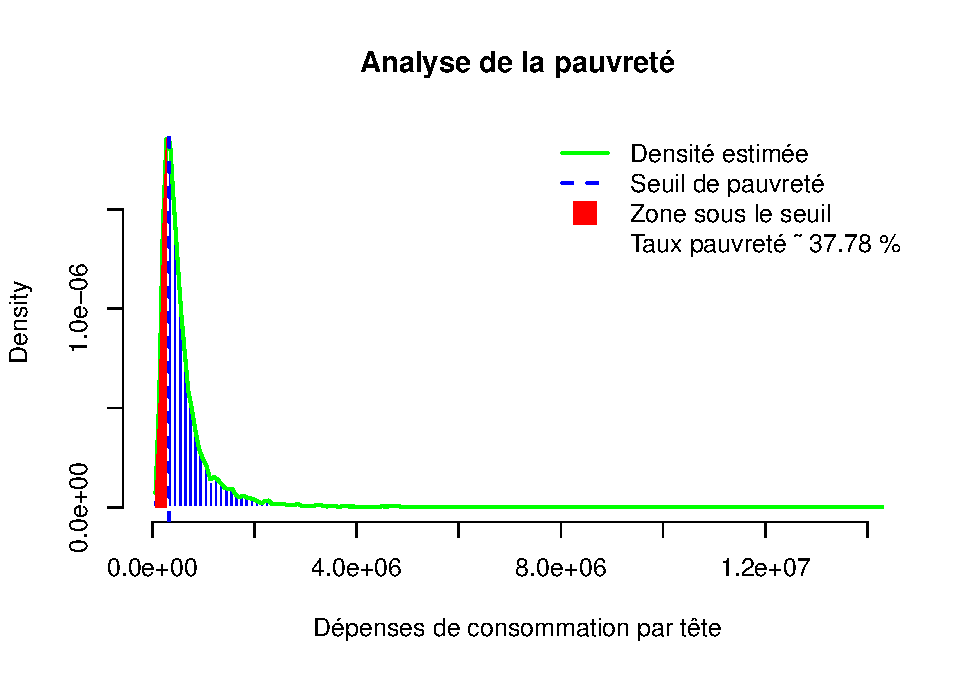
\includegraphics{Stat_non_para_files/figure-latex/unnamed-chunk-179-1.pdf}

\begin{itemize}
\tightlist
\item
  \textbf{Affichage en console}
\end{itemize}

\begin{Shaded}
\begin{Highlighting}[]
\FunctionTok{cat}\NormalTok{(}\StringTok{"Taux de pauvreté estimé :"}\NormalTok{, }\FunctionTok{round}\NormalTok{(taux\_pauvrete }\SpecialCharTok{*} \DecValTok{100}\NormalTok{, }\DecValTok{2}\NormalTok{), }\StringTok{"\%}\SpecialCharTok{\textbackslash{}n}\StringTok{"}\NormalTok{)}
\end{Highlighting}
\end{Shaded}

\begin{verbatim}
## Taux de pauvreté estimé : 37.78 %
\end{verbatim}

\subsubsection{Noyau d'Épanchnikov}\label{noyau-duxe9panchnikov}

La fonction du noyau d'Épanchnikov est définie comme suit :

\[
K(u) =
\begin{cases}
\frac{3}{4}(1 - u^2) & \text{si } |u| \leq 1 \\
0 & \text{sinon}
\end{cases}
\]

\begin{Shaded}
\begin{Highlighting}[]
\NormalTok{epanechnikov\_kernel }\OtherTok{\textless{}{-}} \ControlFlowTok{function}\NormalTok{(u) \{}
\NormalTok{  k }\OtherTok{\textless{}{-}} \FloatTok{0.75} \SpecialCharTok{*}\NormalTok{ (}\DecValTok{1} \SpecialCharTok{{-}}\NormalTok{ u}\SpecialCharTok{\^{}}\DecValTok{2}\NormalTok{) }\SpecialCharTok{*}\NormalTok{ (}\FunctionTok{abs}\NormalTok{(u) }\SpecialCharTok{\textless{}=} \DecValTok{1}\NormalTok{)}
  \FunctionTok{return}\NormalTok{(k)}
\NormalTok{\}}
\end{Highlighting}
\end{Shaded}

\begin{itemize}
\tightlist
\item
  \textbf{Fonction d'estimation de noyau}
\end{itemize}

L'estimateur de la densité à noyau basé sur un échantillon
\(X_1, X_2, \dots, X_n\) est défini par :

\[
\hat{f}_h(x) = \frac{1}{n h} \sum_{i=1}^n K\left( \frac{x - X_i}{h} \right)
\]

\begin{itemize}
\tightlist
\item
  \textbf{Estimateur avec le noyau d'Épanchnikov}
\end{itemize}

En remplaçant \(K(u)\) par le noyau d'Épanchnikov, on obtient :

\[
\hat{f}_h(x) = \frac{1}{n h} \sum_{i=1}^n \left[ \frac{3}{4} \left( 1 - \left( \frac{x - X_i}{h} \right)^2 \right) \cdot \mathbf{1}_{\left| \frac{x - X_i}{h} \right| \leq 1} \right]
\]

\begin{itemize}
\tightlist
\item
  \textbf{Optimisation de h}
\end{itemize}

\emph{Largeur de bande optimale \(h^*\) : }

En minimisant l'AMISE (erreur quadratique intégrée moyenne
asymptotique), on obtient la \textbf{largeur de bande optimale} :

\[
h^* = \left( \frac{R(K)}{ \mu_2^2(K) \cdot R(f'') \cdot n } \right)^{1/5}
\]

\emph{Pour le noyau d'Épanchnikov : }

\[
R(K) = \int_{-1}^1 K^2(u)\, du = \frac{3}{5}, \quad \mu_2(K) = \int_{-1}^1 u^2 K(u)\, du = \frac{1}{5}
\]

En remplaçant dans la formule de \(h^*\), on obtient :

\[
h^* = \left( \frac{\frac{3}{5}}{ \left( \frac{1}{5} \right)^2 \cdot R(f'') \cdot n } \right)^{1/5}
= \left( \frac{3}{5} \cdot \frac{25}{1} \cdot \frac{1}{R(f'') \cdot n} \right)^{1/5}
= \left( \frac{15}{R(f'') \cdot n} \right)^{1/5}
\]

Nous ne connaissons pas la valeur de R(f'\,'). La règle de Silverman
fournit une approximation pratique de la largeur de bande \(h\) pour
l'estimateur de densité à noyau, lorsque la densité \(f\) est supposée
proche d'une loi normale.

La formule est donnée par :

\[
h_{\text{Silverman}} = 0{,}9 \cdot \min\left( \sigma, \frac{\text{IQR}}{1{,}34} \right) \cdot n^{-1/5}
\]

\begin{Shaded}
\begin{Highlighting}[]
\NormalTok{h\_optimal }\OtherTok{\textless{}{-}} \ControlFlowTok{function}\NormalTok{(data) \{}
\NormalTok{  n }\OtherTok{\textless{}{-}} \FunctionTok{length}\NormalTok{(data)}
\NormalTok{  sigma }\OtherTok{\textless{}{-}} \FunctionTok{sd}\NormalTok{(data)}
\NormalTok{  iqr }\OtherTok{\textless{}{-}} \FunctionTok{IQR}\NormalTok{(data)}
\NormalTok{  s }\OtherTok{\textless{}{-}} \FunctionTok{min}\NormalTok{(sigma, iqr }\SpecialCharTok{/} \FloatTok{1.34}\NormalTok{)}
\NormalTok{  h }\OtherTok{\textless{}{-}} \FloatTok{0.9} \SpecialCharTok{*}\NormalTok{ s }\SpecialCharTok{*}\NormalTok{ n}\SpecialCharTok{\^{}}\NormalTok{(}\SpecialCharTok{{-}}\DecValTok{1}\SpecialCharTok{/}\DecValTok{5}\NormalTok{)}
  \FunctionTok{return}\NormalTok{(h)}
\NormalTok{\}}
\end{Highlighting}
\end{Shaded}

\begin{itemize}
\tightlist
\item
  \textbf{Pratique}
\end{itemize}

\begin{Shaded}
\begin{Highlighting}[]
\NormalTok{data }\OtherTok{\textless{}{-}} \FunctionTok{c}\NormalTok{(}\FloatTok{2.1}\NormalTok{, }\FloatTok{2.3}\NormalTok{, }\FloatTok{1.9}\NormalTok{, }\FloatTok{2.5}\NormalTok{, }\FloatTok{1.7}\NormalTok{, }\FloatTok{2.8}\NormalTok{, }\FloatTok{1.1}\NormalTok{, }\FloatTok{3.2}\NormalTok{, }\FloatTok{3.9}\NormalTok{, }\FloatTok{2.9}\NormalTok{)}
\CommentTok{\# Estimation de la densité}
\NormalTok{dens }\OtherTok{\textless{}{-}} \FunctionTok{density}\NormalTok{(data)}

\CommentTok{\# Tracé de la densité}
\FunctionTok{plot}\NormalTok{(dens, }\AttributeTok{main =} \StringTok{"Estimation de la densité"}\NormalTok{, }\AttributeTok{xlab =} \StringTok{"Valeurs"}\NormalTok{, }\AttributeTok{ylab =} \StringTok{"Densité"}\NormalTok{, }\AttributeTok{col =} \StringTok{"blue"}\NormalTok{, }\AttributeTok{lwd =} \DecValTok{2}\NormalTok{)}
\end{Highlighting}
\end{Shaded}

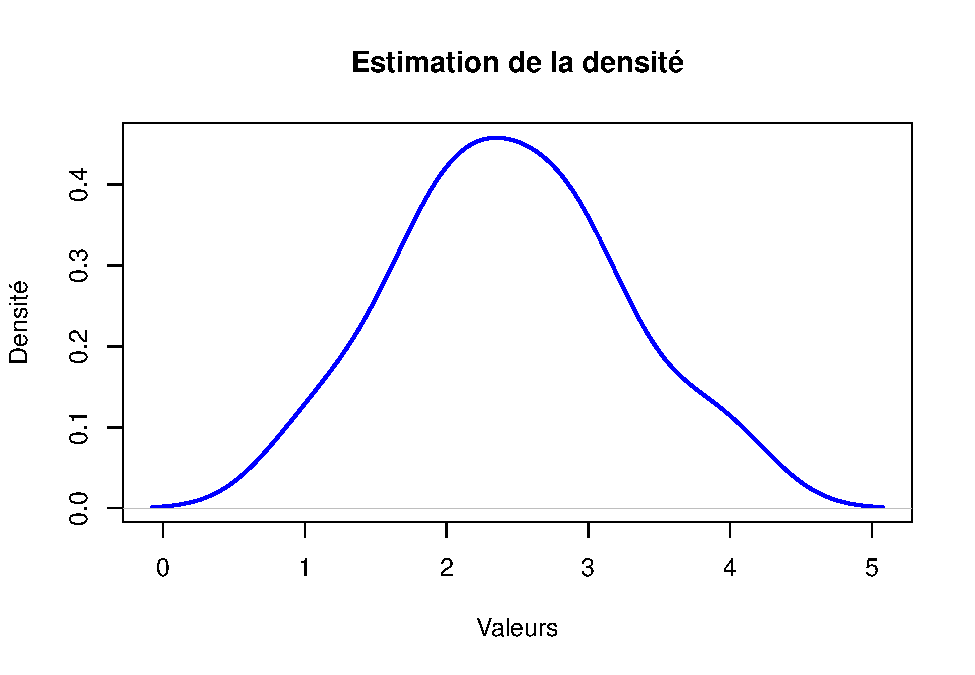
\includegraphics{Stat_non_para_files/figure-latex/unnamed-chunk-182-1.pdf}

\begin{Shaded}
\begin{Highlighting}[]
\CommentTok{\# Génération de données simulées}


\CommentTok{\# Points où on évalue la densité}
\NormalTok{x }\OtherTok{\textless{}{-}} \FunctionTok{seq}\NormalTok{(}\FunctionTok{min}\NormalTok{(data) }\SpecialCharTok{{-}} \DecValTok{1}\NormalTok{, }\FunctionTok{max}\NormalTok{(data) }\SpecialCharTok{+} \DecValTok{1}\NormalTok{, }\AttributeTok{length.out =} \DecValTok{200}\NormalTok{)}

\CommentTok{\# Largeur de bande}
\NormalTok{h }\OtherTok{\textless{}{-}} \FunctionTok{h\_optimal}\NormalTok{(data)}

\CommentTok{\# Calcul de la densité}
\NormalTok{density\_values }\OtherTok{\textless{}{-}} \FunctionTok{epanechnikov\_density}\NormalTok{(x, data, h)}

\CommentTok{\# Affichage du résultat}
\FunctionTok{plot}\NormalTok{(x, density\_values, }\AttributeTok{type =} \StringTok{"l"}\NormalTok{, }\AttributeTok{lwd =} \DecValTok{2}\NormalTok{, }\AttributeTok{col =} \StringTok{"blue"}\NormalTok{,}
     \AttributeTok{main =} \StringTok{"Estimation de densité {-} noyau d\textquotesingle{}Épanchnikov"}\NormalTok{,}
     \AttributeTok{xlab =} \StringTok{"x"}\NormalTok{, }\AttributeTok{ylab =} \StringTok{"Densité"}\NormalTok{)}
\FunctionTok{rug}\NormalTok{(data)  }\CommentTok{\# Ajoute les observations sur l’axe x}
\end{Highlighting}
\end{Shaded}

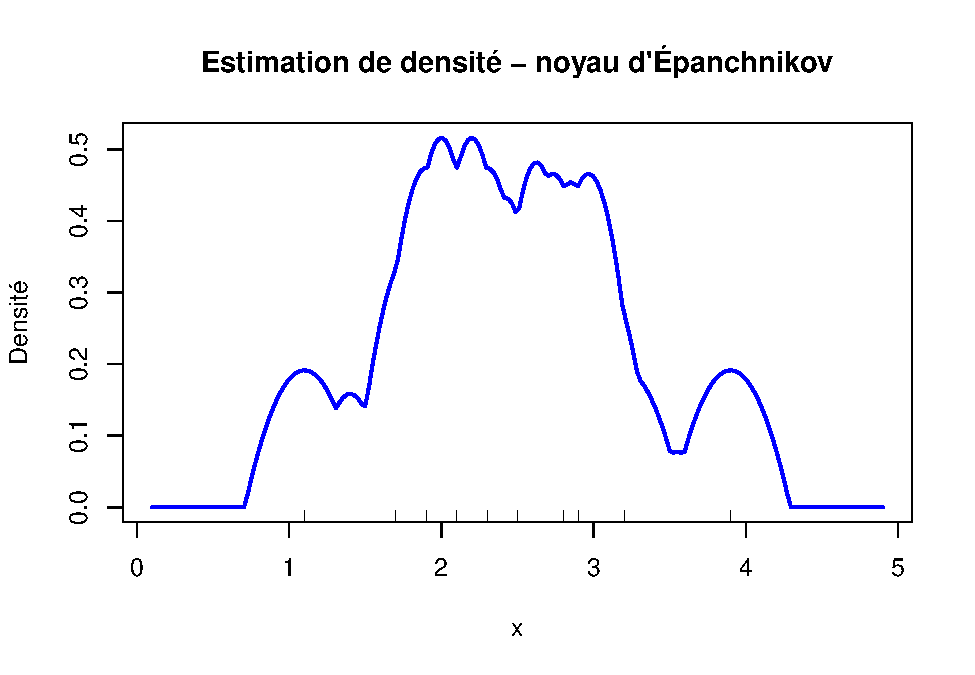
\includegraphics{Stat_non_para_files/figure-latex/unnamed-chunk-183-1.pdf}

\subsubsection{Noyau Biweight}\label{noyau-biweight}

\textbf{Partie théorique}

\begin{itemize}
\tightlist
\item
  \textbf{Échantillon utilisé}
\end{itemize}

\[
X = (1.1,\ 2.3,\ 1.7,\ 2.8,\ 3.2,\ 1.9,\ 2.5,\ 3.7,\ 2.9,\ 2.1)
\]

\begin{itemize}
\tightlist
\item
  \textbf{Noyau Biweight}
\end{itemize}

\[
K(x) =
\begin{cases}
\dfrac{15}{16} \times (1 - x^2)^2 & \text{si } |x| < 1 \\
0 & \text{sinon}
\end{cases}
\]

\begin{itemize}
\tightlist
\item
  \textbf{Estimateur de la densité par noyau Biweight}
\end{itemize}

\[
\hat{f}_n(x) = \dfrac{1}{n h} \sum_{i=1}^{n} K\left( \dfrac{x - X_i}{h} \right)
\]

où \(h\) est la fenêtre de lissage.

\textbf{Application}

\begin{itemize}
\tightlist
\item
  \textbf{Données}
\end{itemize}

\begin{Shaded}
\begin{Highlighting}[]
\DocumentationTok{\#\#\# Chargement des données}
\NormalTok{X }\OtherTok{\textless{}{-}} \FunctionTok{c}\NormalTok{(}\FloatTok{1.1}\NormalTok{, }\FloatTok{2.3}\NormalTok{, }\FloatTok{1.7}\NormalTok{, }\FloatTok{2.8}\NormalTok{, }\FloatTok{3.2}\NormalTok{, }\FloatTok{1.9}\NormalTok{, }\FloatTok{2.5}\NormalTok{, }\FloatTok{3.7}\NormalTok{, }\FloatTok{2.9}\NormalTok{, }\FloatTok{2.1}\NormalTok{)}
\end{Highlighting}
\end{Shaded}

\begin{itemize}
\tightlist
\item
  \textbf{Définition du noyau Biweight}
\end{itemize}

\begin{Shaded}
\begin{Highlighting}[]
\CommentTok{\# Fonction noyau Biweight}
\NormalTok{biweight\_kernel }\OtherTok{\textless{}{-}} \ControlFlowTok{function}\NormalTok{(x) \{}
  \FunctionTok{ifelse}\NormalTok{(}\FunctionTok{abs}\NormalTok{(x) }\SpecialCharTok{\textless{}} \DecValTok{1}\NormalTok{, (}\DecValTok{15}\SpecialCharTok{/}\DecValTok{16}\NormalTok{) }\SpecialCharTok{*}\NormalTok{ (}\DecValTok{1} \SpecialCharTok{{-}}\NormalTok{ x}\SpecialCharTok{\^{}}\DecValTok{2}\NormalTok{)}\SpecialCharTok{\^{}}\DecValTok{2}\NormalTok{, }\DecValTok{0}\NormalTok{)}
\NormalTok{\}}
\end{Highlighting}
\end{Shaded}

\begin{itemize}
\tightlist
\item
  \textbf{Estimation de la densité}
\end{itemize}

\begin{Shaded}
\begin{Highlighting}[]
\CommentTok{\# Fonction d\textquotesingle{}estimation de la densité}
\NormalTok{density\_estimate }\OtherTok{\textless{}{-}} \ControlFlowTok{function}\NormalTok{(x, sample, h) \{}
\NormalTok{  n }\OtherTok{\textless{}{-}} \FunctionTok{length}\NormalTok{(sample)}
\NormalTok{  sum }\OtherTok{\textless{}{-}} \DecValTok{0}
  \ControlFlowTok{for}\NormalTok{ (i }\ControlFlowTok{in} \DecValTok{1}\SpecialCharTok{:}\NormalTok{n) \{}
\NormalTok{    sum }\OtherTok{\textless{}{-}}\NormalTok{ sum }\SpecialCharTok{+} \FunctionTok{biweight\_kernel}\NormalTok{((x }\SpecialCharTok{{-}}\NormalTok{ sample[i]) }\SpecialCharTok{/}\NormalTok{ h)}
\NormalTok{  \}}
  \FunctionTok{return}\NormalTok{(sum }\SpecialCharTok{/}\NormalTok{ (n }\SpecialCharTok{*}\NormalTok{ h))}
\NormalTok{\}}
\end{Highlighting}
\end{Shaded}

\begin{itemize}
\tightlist
\item
  \textbf{Calcul des densités estimées}
\end{itemize}

\begin{Shaded}
\begin{Highlighting}[]
\CommentTok{\# Définition de la fenêtre de lissage}
\NormalTok{h }\OtherTok{\textless{}{-}} \FloatTok{0.5}

\CommentTok{\# Calcul des densités estimées pour chaque observation}
\NormalTok{density\_estimates }\OtherTok{\textless{}{-}} \FunctionTok{sapply}\NormalTok{(X, density\_estimate, }\AttributeTok{sample =}\NormalTok{ X, }\AttributeTok{h =}\NormalTok{ h)}

\CommentTok{\# Affichage des densités estimées}
\NormalTok{density\_estimates}
\end{Highlighting}
\end{Shaded}

\begin{verbatim}
##  [1] 0.1875 0.4764 0.3441 0.4614 0.2886 0.4764 0.4452 0.1875 0.4614 0.5007
\end{verbatim}

\begin{itemize}
\tightlist
\item
  \textbf{Visualisation : Histogramme des densités estimées}
\end{itemize}

\begin{Shaded}
\begin{Highlighting}[]
\FunctionTok{hist}\NormalTok{(density\_estimates,}
     \AttributeTok{main =} \StringTok{"Histogramme des densités estimées"}\NormalTok{,}
     \AttributeTok{xlab =} \StringTok{"Densité estimée"}\NormalTok{,}
     \AttributeTok{col =} \StringTok{"lightblue"}\NormalTok{,}
     \AttributeTok{border =} \StringTok{"black"}\NormalTok{)}
\end{Highlighting}
\end{Shaded}

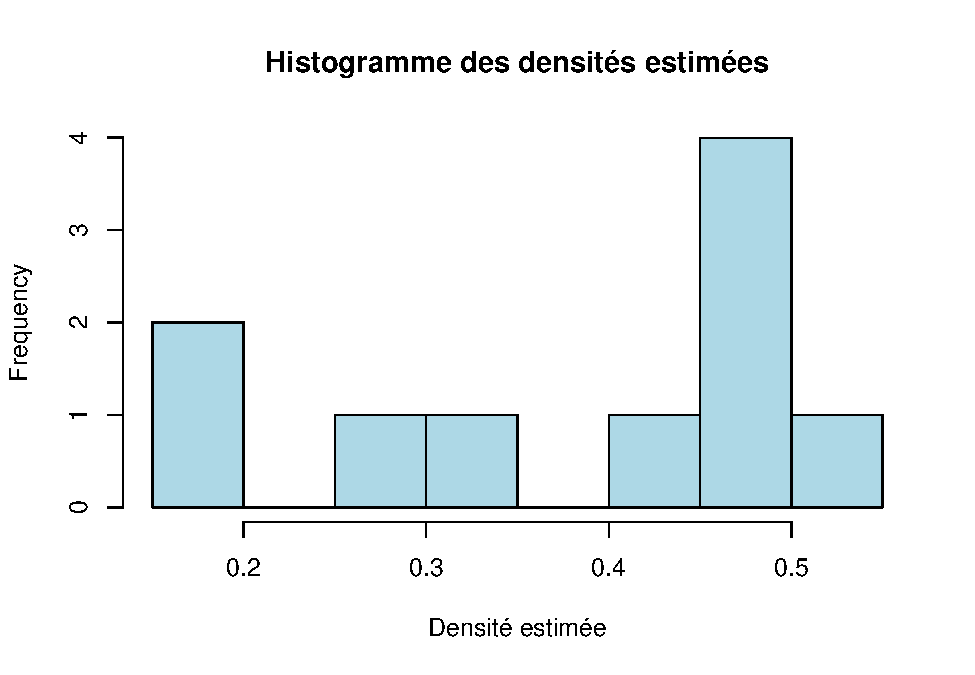
\includegraphics{Stat_non_para_files/figure-latex/unnamed-chunk-188-1.pdf}

\textbf{Utilisation du test de Wald pour tester l'égalité de la densité
estimée avec la densité uniforme}

\begin{itemize}
\tightlist
\item
  \textbf{Hypothèse du test}
\end{itemize}

\[
\begin{cases}
H_0 : \text{La densité de } X \text{ est uniforme} \\
H_1 : \text{La densité de } X \text{ n'est pas uniforme}
\end{cases}
\]

\begin{itemize}
\tightlist
\item
  \textbf{Région de rejet}
\end{itemize}

Pour un test bilatéral de Wald au seuil \(\alpha = 5\%\), les valeurs
critiques \(c_1\) et \(c_2\) sont déterminées telles que :

\[
P\left( \hat{f}_n(x) < c_1 \right) = \dfrac{\alpha}{2} \quad \text{et} \quad P\left( \hat{f}_n(x) > c_2 \right) = \dfrac{\alpha}{2}
\]

\begin{itemize}
\tightlist
\item
  \textbf{Staistique du test}
\end{itemize}

\[
W = \frac{(\hat{f}(x) - f_0(x))^2}{\text{Var}(\hat{f}(x))}
\]

\begin{itemize}
\tightlist
\item
  \textbf{Calcul des statistiques : Moyenne et Variance}
\end{itemize}

\begin{Shaded}
\begin{Highlighting}[]
\CommentTok{\# Calcul de la moyenne}
\NormalTok{mean\_density }\OtherTok{\textless{}{-}} \FunctionTok{mean}\NormalTok{(density\_estimates)}

\CommentTok{\# Calcul de la variance}
\NormalTok{var\_density }\OtherTok{\textless{}{-}} \FunctionTok{var}\NormalTok{(density\_estimates)}

\CommentTok{\# Affichage des résultats}
\FunctionTok{cat}\NormalTok{(}\StringTok{"Moyenne des densités estimées :"}\NormalTok{, mean\_density, }\StringTok{"}\SpecialCharTok{\textbackslash{}n}\StringTok{"}\NormalTok{)}
\end{Highlighting}
\end{Shaded}

\begin{verbatim}
## Moyenne des densités estimées : 0.38292
\end{verbatim}

\begin{Shaded}
\begin{Highlighting}[]
\FunctionTok{cat}\NormalTok{(}\StringTok{"Variance des densités estimées :"}\NormalTok{, var\_density, }\StringTok{"}\SpecialCharTok{\textbackslash{}n}\StringTok{"}\NormalTok{)}
\end{Highlighting}
\end{Shaded}

\begin{verbatim}
## Variance des densités estimées : 0.01492526
\end{verbatim}

\begin{itemize}
\tightlist
\item
  \textbf{Test statistique et décision}
\end{itemize}

\begin{Shaded}
\begin{Highlighting}[]
\CommentTok{\# Calcul de la statistique de test}
\NormalTok{test\_statistic }\OtherTok{\textless{}{-}}\NormalTok{ (mean\_density }\SpecialCharTok{{-}} \DecValTok{1}\NormalTok{) }\SpecialCharTok{/} \FunctionTok{sqrt}\NormalTok{(var\_density }\SpecialCharTok{/} \FunctionTok{length}\NormalTok{(density\_estimates))}

\CommentTok{\# Calcul de la valeur critique pour un test bilatéral à 5\%}
\NormalTok{alpha }\OtherTok{\textless{}{-}} \FloatTok{0.05}
\NormalTok{critical\_value }\OtherTok{\textless{}{-}} \FunctionTok{qnorm}\NormalTok{(}\DecValTok{1} \SpecialCharTok{{-}}\NormalTok{ alpha }\SpecialCharTok{/} \DecValTok{2}\NormalTok{)}

\CommentTok{\# Affichage de la statistique de test et de la valeur critique}
\FunctionTok{cat}\NormalTok{(}\StringTok{"Statistique de test :"}\NormalTok{, test\_statistic, }\StringTok{"}\SpecialCharTok{\textbackslash{}n}\StringTok{"}\NormalTok{)}
\end{Highlighting}
\end{Shaded}

\begin{verbatim}
## Statistique de test : -15.97278
\end{verbatim}

\begin{Shaded}
\begin{Highlighting}[]
\FunctionTok{cat}\NormalTok{(}\StringTok{"Valeur critique :"}\NormalTok{, critical\_value, }\StringTok{"}\SpecialCharTok{\textbackslash{}n}\StringTok{"}\NormalTok{)}
\end{Highlighting}
\end{Shaded}

\begin{verbatim}
## Valeur critique : 1.959964
\end{verbatim}

\begin{Shaded}
\begin{Highlighting}[]
\CommentTok{\# Prise de décision}
\ControlFlowTok{if}\NormalTok{ (}\FunctionTok{abs}\NormalTok{(test\_statistic) }\SpecialCharTok{\textgreater{}}\NormalTok{ critical\_value) \{}
  \FunctionTok{cat}\NormalTok{(}\StringTok{"Nous rejetons l\textquotesingle{}hypothèse nulle (H0).}\SpecialCharTok{\textbackslash{}n}\StringTok{"}\NormalTok{)}
\NormalTok{\} }\ControlFlowTok{else}\NormalTok{ \{}
  \FunctionTok{cat}\NormalTok{(}\StringTok{"Nous ne rejetons pas l\textquotesingle{}hypothèse nulle (H0).}\SpecialCharTok{\textbackslash{}n}\StringTok{"}\NormalTok{)}
\NormalTok{\}}
\end{Highlighting}
\end{Shaded}

\begin{verbatim}
## Nous rejetons l'hypothèse nulle (H0).
\end{verbatim}

\end{document}
